%-------------------------------------------------------------------------------
% This file provides a skeleton ATLAS note.
% \pdfinclusioncopyfonts=1
% This command may be needed in order to get \ell in PDF plots to appear. Found in
% https://tex.stackexchange.com/questions/322010/pdflatex-glyph-undefined-symbols-disappear-from-included-pdf
%-------------------------------------------------------------------------------
% Specify where ATLAS LaTeX style files can be found.
\newcommand*{\ATLASLATEXPATH}{latex/}
% Use this variant if the files are in a central location, e.g. $HOME/texmf.
% \newcommand*{\ATLASLATEXPATH}{}
%-------------------------------------------------------------------------------
\documentclass[NOTE, atlasdraft=true, texlive=2016, UKenglish]{\ATLASLATEXPATH atlasdoc}
% The language of the document must be set: usually UKenglish or USenglish.
% british and american also work!
% Commonly used options:
%  atlasdraft=true|false This document is an ATLAS draft.
%  texlive=YYYY          Specify TeX Live version (2016 is default).
%  coverpage             Create ATLAS draft cover page for collaboration circulation.
%                        See atlas-draft-cover.tex for a list of variables that should be defined.
%  cernpreprint          Create front page for a CERN preprint.
%                        See atlas-preprint-cover.tex for a list of variables that should be defined.
%  NOTE                  The document is an ATLAS note (draft).
%  PAPER                 The document is an ATLAS paper (draft).
%  CONF                  The document is a CONF note (draft).
%  PUB                   The document is a PUB note (draft).
%  BOOK                  The document is of book form, like an LOI or TDR (draft)
%  txfonts=true|false    Use txfonts rather than the default newtx
%  paper=a4|letter       Set paper size to A4 (default) or letter.

%-------------------------------------------------------------------------------
% Extra packages:
\usepackage[]{\ATLASLATEXPATH atlaspackage}
% Commonly used options:
%  biblatex=true|false   Use biblatex (default) or bibtex for the bibliography.
%  backend=bibtex        Use the bibtex backend rather than biber.
%  subfigure|subfig|subcaption  to use one of these packages for figures in figures.
%  minimal               Minimal set of packages.
%  default               Standard set of packages.
%  full                  Full set of packages.
%-------------------------------------------------------------------------------
% Style file with biblatex options for ATLAS documents.
\usepackage{\ATLASLATEXPATH atlasbiblatex}

% Package for creating list of authors and contributors to the analysis.
\usepackage{\ATLASLATEXPATH atlascontribute}

% Useful macros
\usepackage{\ATLASLATEXPATH atlasphysics}
% See doc/atlas_physics.pdf for a list of the defined symbols.
% Default options are:
%   true:  journal, misc, particle, unit, xref
%   false: BSM, heppparticle, hepprocess, hion, jetetmiss, math, process, other, texmf
% See the package for details on the options.

% Files with references for use with biblatex.
% Note that biber gives an error if it finds empty bib files.
\addbibresource{ANA-HDBS-2020-09-INT1.bib}
\addbibresource{bib/ATLAS.bib}
\addbibresource{bib/CMS.bib}
\addbibresource{bib/ConfNotes.bib}
\addbibresource{bib/PubNotes.bib}
\addbibresource{bib/ATLAS-useful.bib}

% Paths for figures - do not forget the / at the end of the directory name.
\graphicspath{{logos/}{figures/}}

% Add you own definitions here (file ANA-HDBS-2020-09-INT1-defs.sty).
\usepackage{tikz-feynhand}
\usepackage{here}
\usepackage{dcolumn}
\usepackage{scalefnt}
\usepackage{ANA-HDBS-2020-09-INT1-defs}
\usepackage{color}
\usepackage{multirow}
%% \usepackage[hang,small,bf]{caption}
%% \usepackage[subrefformat=parens]{subcaption}
%% \captionsetup{compatibility=false}

%-------------------------------------------------------------------------------
% Generic document information
%-------------------------------------------------------------------------------

% Title, abstract and document
%-------------------------------------------------------------------------------
% This file contains the title, author and abstract.
% It also contains all relevant document numbers used for an ATLAS note.
%-------------------------------------------------------------------------------

% Title
\AtlasTitle{Search for $tb$ resonance using boosted top-quark topology in the lepton+jets final state at $\sqrt{s}=13$ TeV with the ATLAS detector}

% Draft version:
% Should be 1.0 for the first circulation, and 2.0 for the second circulation.
% If given, adds draft version on front page, a 'DRAFT' box on top of each other page, 
% and line numbers.
% Comment or remove in final version.
\AtlasVersion{0.1}

% Abstract - % directly after { is important for correct indentation
\AtlasAbstract{
A search for $tb$ resonances with a boosted top tagging technique is presented, focusing on a final state consisting of a single charged lepton and multiple jets as well as a top-tagged large-$R$ jet. The analysis is based on the pp collision data at the centre-of-mass energy of 13 TeV collected with the ATLAS detector with an integrated luminosity of 139 $\text{fb}^{-1}$. As a hypothetical particle with spin-0(1), a charged Higgs boson (a $W'$ boson) scenario is searched in the mass range from 1 TeV up to 5 TeV.
}

% Author - this does not work with revtex (add it after \begin{document})
% \author{The ATLAS Collaboration}

% Authors and list of contributors to the analysis
% \AtlasAuthorContributor also adds the name to the author list
% Include package latex/atlascontribute to use this
% Use authblk package if there are multiple authors, which is included by latex/atlascontribute
\usepackage{authblk}
% Use the following 3 lines to have all institutes on one line
% \makeatletter
% \renewcommand\AB@affilsepx{, \protect\Affilfont}
% \makeatother
\renewcommand\Authands{, } % avoid ``. and'' for last author
\renewcommand\Affilfont{\itshape\small} % affiliation formatting
\AtlasAuthorContributor{De La Torre Perez, Hector}{a}{W' vs H+ comparisons, W' generation}
\AtlasAuthorContributor{Gombas, Jason Peter}{a}{W' NLO model, W' vs H+ comparisons, W'generation}
\AtlasAuthorContributor{Schwienhorst, Reinhard}{a}{W' NLO model, Jason supervision}
\AtlasAuthorContributor{Sato, Koji}{b}{Analysis contact, supervision of Hiroki}
\AtlasAuthorContributor{Hirose, Shigeki}{b}{Analysis contact, ntuple production, BDT training, MC production, supervision of Hiroki}
\AtlasAuthorContributor{Yamauchi, Hiroki}{b}{Main analyser: ntuple production, fit studies and limits extraction}
\AtlasAuthorContributor{Salvador Salas, Adrian}{c}{Main analyser of resolved analysis, providing technical support; ntuple production}
\AtlasAuthorContributor{Riu, Imma}{c}{Signal AODs and TOPQ1s production; provision of other technical support from resolved analysis}
\AtlasAuthorContributor{Mir Martinez, Lluisa Maria}{c}{Monte Carlo production}
\affil[a]{Michigan State University (US)}
\affil[b]{University of Tsukuba (JP)}
\affil[c]{The Barcelona Institute of Science and Technology (BIST) (ES)}


% \AtlasAuthorContributor{First AtlasAuthorContributor}{a}{Author's contribution.}
% \AtlasAuthorContributor{Second AtlasAuthorContributor}{b}{Author's contribution.}
% \AtlasAuthorContributor{Third AtlasAuthorContributor}{a}{Author's contribution.}
% \AtlasContributor{Fourth AtlasContributor}{Contribution to the analysis.}
%\author[a]{Hiroki Yamaichi}
%\author[a]{Shigeki Hirose}
%\author[b]{Llu\"{i}sa-Maria Mir}
%\author[b]{Imma Riu}
%\author[b]{Adrian Salvador}
%\author[a]{Koji Sato}

%\affil[a]{University of Tsukuba, Japan}
%\affil[b]{Institut de F\'{i}sica d'Altes Energies, Barcelona, Spain}
%\affil[b]{Another Institution}


% If a special author list should be indicated via a link use the following code:
% Include the two lines below if you do not use atlasstyle:
% \usepackage[marginal,hang]{footmisc}
% \setlength{\footnotemargin}{0.5em}
% Use the following lines in all cases:
% \usepackage{authblk}
% \author{The ATLAS Collaboration%
% \thanks{The full author list can be found at:\newline
%   \url{https://atlas.web.cern.ch/Atlas/PUBNOTES/ATL-PHYS-PUB-2016-007/authorlist.pdf}}
% }

% ATLAS reference code, to help ATLAS members to locate the paper
\AtlasRefCode{ANA-HDBS-2020-09}

% ATLAS note number. Can be an COM, INT, PUB or CONF note
\AtlasNote{ANA-HDBS-2020-09-INT1}

% Author and title for the PDF file
\hypersetup{pdftitle={ATLAS document},pdfauthor={The ATLAS Collaboration}}

%-------------------------------------------------------------------------------
% Content
%-------------------------------------------------------------------------------
\begin{document}

\maketitle

\setcounter{tocdepth}{3}
\tableofcontents
\clearpage

% List of contributors - print here or after the Bibliography.
\PrintAtlasContribute{0.30}
\clearpage

%----------------------------------------------------------------------
\textbf{Remaining to do}

\begin{description}

\item[The reweighting method:] A complete proposal is to be discussed at the EB request (HBSM meeting) on 21st July, and incorporate comments and discussions there for the method, summarize them in the note in 1-2 weeks after the meeting.

\item[$W'$ MC production:] Validations are to be finalized by the end of July so that the MC generator can be implemented into the ATLAS official software. We aim for finishing the MC production as well as limit evaluations by the end of September. This is to be done in parallel to EB review, as agreed with the HBSM / HDBS conveners.

\item[Theoretical interpretation: ] Interpret limits in terms of the theoretical H+/W' scenarios, such as hMSSM and XXX. This will be done by the end of September.

\end{description}

\textbf{Version log with major updates:}


\clearpage
%----------------------------------------------------------------------

%---- Section 1
\section{Introduction}
\label{sec:Introduction}

The discovery of a neutral boson with a measured mass around 125 GeV at the Large Hadron Collider (LHC) in 2012 \cite{HIGG-2012-27, CMS-HIG-12-028, HIGG-2014-14} opens the question whether this is the Higgs boson of the Standard Model (SM) or part of an extended scalar sector. Indeed, charged Higgs bosons \footnote{Charge-conjugate is implied elsewhere in this note.} are predicted in several extensions of the SM, which add a second doublet \cite{T.D.Lee-1973, G.Branco-2012, K.Inoue-1982, T.Cheng-1989} or triplets \cite{T.Cheng-1989, J.Schechter-1980, G.Lazarides-1981, R.N.Mohapatra-1981, M.Magg-1980} to its scalar sector. In CP-conserving Two-Higgs-Doublet Models (2HDMs) $H^{+}$ production and decay at tree level depend on its mass and two parameters: the mixing angle $\alpha$ of the neutral CP-even Higgs bosons, and the ratio of the vacuum expectation values of the two Higgs doublets ($\tan{\beta}$).

\begin{figure}[H]
  \centering
  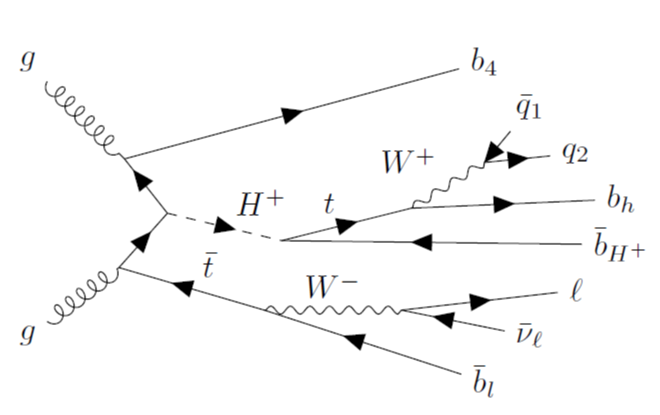
\includegraphics[keepaspectratio,scale=0.5]{images/Introduction/FeynmanDiagram_Htb.png}
  \caption{Feynman diagram for $pp{\rightarrow}tbH^{+}{\rightarrow}tb(tb)$}
  \label{fig:FeynmanDiagram_Htb}
\end{figure}


\vskip.2\baselineskip

For $H^{+}$ masses above the top-quark mass the leading production mode is $gg{\rightarrow}tbH^{+}$ and, close to the alignment limit when $\cos{({\beta}-{\alpha})}{\approx}0$, the dominant decay mode is $H^{+}{\rightarrow}tb$. For lower $H^{+}$ masses, the dominant decay mode is $H^{+}{\rightarrow}{\tau}{\nu}$, as well as for large values of $\tan{\beta}$ irrespective of the charged Higgs mass. Therefore, the two decay modes naturally complement each other in searches for charged Higgs bosons.

\vskip.2\baselineskip

The ATLAS and CMS collaborations have searched for charged Higgs bosons in $pp$ collisions at $\sqrt{s}=7,8$ and 13 TeV, probing the mass range below the top-quark mass in the $\tau\nu$ \cite{HIGG-2012-09, HIGG-2012-22, HIGG-2013-30, CMS-HIG-11-019, CMS-HIG-14-023, HIGG-2016-11}, $cs$ \cite{HIGG-2012-10, CMS-HIG-13-035}, and $cb$ \cite{CMS-HIG-16-030} decay modes, as well as above the top-quark mass in the $\tau\nu$ and $tb$ decay modes \cite{HIGG-2013-30, CMS-HIG-14-023, HIGG-2016-11, HIGG-2013-28, HIGG-2015-11, HIGG-2017-04, HDBS-2021-02, CMS-HIG-18-004, CMS-HIG-18-015, EXOT-2018-32}. In addition, $H^{+}{\rightarrow}WZ$ was searched for in the vector-boson-fusion production mode \cite{HIGG-2014-13, CMS-HIG-16-027}. No evidence for charged Higgs bosons was found in any of these searches.

\vskip.2\baselineskip

This note presents a search for $H^{+}$ production in the $H^{+}{\rightarrow}tb$ decay mode using $pp$ collisions at $\sqrt{s}=13$ TeV. Events with one charged lepton ($l=e,\mu$) and jets in the final state are considered. Compared with the previous analysis using the same final state and the dataset \cite{HDBS-2021-02} (so-called `resolved analysis), boosted top tagging technique is used to identify a hadoronically decaying top quark originated from the decay of the heavy $H^{+}$. This technique allows to improve sensitivities in the high mass regions, where all top decay products are merged into a single large-R jet, and therefore cannot be reconstructed in the resolved analysis \cite{HDBS-2021-02}. 
%Exclusive regions are defined according to the number of jets tagged as originating from the hadronisation of a top quark and $b$-quark.
To separate signal from SM background, multivariate discriminants are employed in the regions where the signal rate is expected to be the largest. Limits on the $H^{+}{\rightarrow}tb$ production cross-section are set by a simultaneous fit of BDT distributions.

\vskip.2\baselineskip

Furthermore, the analysis technique is extended to a search for the $W'{\rightarrow}tb$ decay, where $W'$ is produced in association with $tb$. Several theories beyond the SM predict heavy-charged gauge bosons, which are usually referred to as $W'$ bosons\cite{dienes1999grand,weinberg1979implications,susskind1979dynamics,dimopoulos1979mass,eichten1980dynamical,muller1996topflavor}. Such $W'$ bosons can be heavy enough to decay into a top quark and a bottom quark. Some models predict $W'$ bosons that preferably couple to quarks or third-generation fermions \cite{burdman2006resonances,malkawi1996model,pati1974lepton,hill1995topcolor}. Unlike the $W$ boson, which only couples to left-handed fermions, the chirality of the interaction of the $W'$ boson can be left or right-handed, or a mixture of the two. In models where the right-handed neutrinos are heavier than the right-handed $W'$ boson, such $W'$ bosons cannot be searched for in the leptonic decay modes. We search for $W'$ bosons produced in association with a top quark and a bottom quark, as illustrated in Figure \ref{fig:Wprime_diagram}.

Formerly, $W'$ bosons decaying into a top quark and a bottom quark were searched for in collisions between a quark and an antiquark of any flavour, where the $W'$ boson is singly produced without a top quark.  D0 \cite{abazov2011search} and CDF \cite{aaltonen2009search} Collaborations at the Tevatron and CMS \cite{CMS-EXO-12-001,CMS-B2G-12-010,CMS-B2G-17-010,CMS-B2G-20-005} and ATLAS \cite{TOPQ-2012-19,EXOT-2013-14,EXOT-2017-02,EXOT-2016-18} experiments at the LHC have published such search results.


The analysis replies on ATLAS official background as well as requested $H^+$ and $W'$ signal samples, as detailed in Section~\ref{sec:DataAndMC}, with the TOPQ1 derivation. The ntuples are produced using the TTHbbAnalysis software package.\footnote{https://gitlab.cern.ch/atlasHTop/TTHbbAnalysis/-/tree/user/hyamauch/pflow\_dev\_HplusBoosted} These ntuples are used as inputs to TRExFitter to perform statistical analysis.\footnote{https://gitlab.cern.ch/hyamauch/TRExFitter}

\clearpage
%----------------------------------------------------------------------

%% %----------------------------------------------------------------------
\section{Data and MonteCarlo Simulated Events}
\label{sec:DataAndMC}

\subsection{Data Sample}
\label{subsec:DataSample}
This analysis uses $pp$ collision data collected from 2015 to 2018 by the ATLAS detector at $\sqrt{s}=13$ TeV. Selected events are recorded using unprescaled triggers, as detailed in Table \ref{tab:GlobalLeptonTriggers}. Only runs with stable colliding beams and all ATLAS subsystems operational are used. These are summarized in the Good Run Lists (GRL) shown in Table \ref{tab:GRLForData}, together with the integrated luminosity collected each year. The total integrated luminosity is 139 $\text{fb}^{-1}$ \cite{ATLAS-CONF-2019-021}.

\begin{table}[H]
  \centering
  \subfloat[] {
    \begin{tabular*}{150mm}{@{\extracolsep{\fill}}cc}
      \hline\hline
      Year & Single-electron triggers\\
      \hline
      \multicolumn{1}{l}{2015} & e24\_lhmedium\_L1EM20VH\_OR\_e60\_lhmedium\_OR\_e120\_lhloose\\
      \multicolumn{1}{l}{2016-2018} & e26\_lhtight\_nod0\_ivarloose\_OR\_e60\_lhmedium\_nod0\_OR\_e140\_lhloose\_nod0\\
      \hline\hline
    \end{tabular*}
    \label{tab:SingleElectronTriggers}
  }\\
  \subfloat[] {
    \begin{tabular*}{100mm}{@{\extracolsep{\fill}}cc}
      \hline\hline
      Year & Single-muon triggers\\
      \hline
      \multicolumn{1}{l}{2015} & mu20\_iloose\_L1MU15\_OR\_mu50\\
      \multicolumn{1}{l}{2016-2018} & mu26\_ivarmedium\_OR\_mu50\\
      \hline\hline
    \end{tabular*}
    \label{tab:SingleMuonTriggers}
  }
  \caption{Single-electron (a) and single-muon (b) trigger menus used depending on the year of data-taking.}
  \label{tab:GlobalLeptonTriggers}
\end{table}

\begin{table}[H]
  \centering
  \begin{tabular*}{150mm}{@{\extracolsep{\fill}}ccc}
    \hline\hline
    Year & Luminosity ($\text{pb}^{-1}$) & GRL\\
    \hline
    2015 & 3219.6  & data15\_13TeV/20170619/physics\_25ns\_21.0.19.xml\\
    2016 & 32988.1 & data16\_13TeV/20180129/physics\_25ns\_21.0.19.xml\\
    2017 & 44307.4 & data17\_13TeV/20180619/physics\_25ns\_Triggerno17e33prim.xml\\
    2018 & 58450.1 & data18\_13TeV/20190318/physics\_25ns\_Triggerno17e33prim.xml\\
    \hline\hline
  \end{tabular*}
  \caption{Integrated luminosity for each year of data-taking, computed with the OflLumi-13TeV-010 luminosity
  tag \cite{LuminosityForPhysis}, together with the corresponding GRLs \cite{GoodRunListRun2}.}
  \label{tab:GRLForData}
\end{table}

\subsection{Signal Samples}
\label{subsec:SignalSample}
This paragraph describes MC samples used for each signal event's estimation. The summary is shown in Table \ref{tab:SigSampleSummary}.

\begin{table}[H]
  \centering
  \begin{tabular*}{160mm}{@{\extracolsep{\fill}}lllll}
    \hline\hline
    Physics process & Generator & PS generator & Normalisation & PDF set\\
    \hline
    $tbH^{+}$ ($M_{H^{+}}\leq3.0$ TeV)  & MG5\_aMC 2.6.2 & Pythia 8.212 & NLO & NNPDF2.3NLO\\
    $tbH^{+}$ ($M_{H^{+}}=4.0,5.0$ TeV) & MG5\_aMC 2.8.1 & Pythia 8.244 & NLO & NNPDF3.0NLO\\
    $tbW'$                              & MG5\_aMC 2.9.9 & Pythia 8.307 & NLO & NNPDF3.0NLO\\
    \hline\hline
  \end{tabular*}
  \caption{Nominal simulated signal event samples. The generator, parton shower generator and cross-section used for normalization are shown together with the applied PDF set.}
  \label{tab:SigSampleSummary}
\end{table}

\subsubsection{$\bar{t}bH^{+}$ Samples}
\label{subsec:HpSample}

\newcounter{Num}
\setcounter{Num}{2}

The $H^{+}$ signal samples are generated with MadGraph5\_aMCatNLO (MG5\_aMC) \cite{C.Degrande-2015}, which is a generator based on a four-flavor scheme (4FS) next-to-leading order (NLO) in QCD \cite{Alwall:2014hca}. The NNPDF2.3NLO \cite{Ball:2012cx} parton distribution function (PDF) set is used. \footnote{The samples with masses of 4 and 5 TeV are generated using NNPDF3.0NLO \cite{Ball:2014uwa} PDF set.} The width of the $H^{+}$ is set to zero. Dynamic QCD factorisation and renormalisation scales ($\mu_{f}$ and $\mu_{r}$) are set to $\frac{1}{3}\sum_{i}\sqrt{m(i)^{2}+p_{T}(i)^{2}}$, where $i$ runs over the final state particles ($H^{+}$, $t$ and $b$) used in the generation. The events are showered with Pythia 8.212 \cite{Sjostrand:2007gs} with the A14 \cite{ATL-PHYS-PUB-2014-021} set of underlying-event related parameters tuned to ATLAS. Ten different $H^{+}$ mass points between 1000 and 5000 GeV are generated as detailed in Table \ref{tab:HpSignalSamples}. The table also shows cross sections from MG5\_aMC and Santander-matched cross sections for 2HDM type-\Roman{Num} (a la MSSM), but without SUSY QCD corrections \cite{C.Degrande-2015, M.Flechl-2015, S.Dittmaier-2011, E.L.Berger-2005}. All samples are fully simulated with the proportions of mc16a, mc16d, and mc16e corresponding to the amount of data recorded in the 2015-2016, 2017, and 2018 data-taking years.

\begin{table}[H]
  \centering
  \begin{tabular*}{160mm}{@{\extracolsep{\fill}}cccccc}
    \hline\hline
    DSID   & $H^{+}$ mass [GeV] & Size & ${\sigma}^{\text{MG5\_aMC}}$ [fb] & ${\sigma}_{\tan{\beta}=1}^{\text{MSSM}}$ [fb] & ${\sigma}_{\tan{\beta}=60}^{\text{MSSM}}$ [fb]\\
    \hline
    450004 & 1000 & 1.0M & 3.28                  & 40.9 & 37.8\\
    450598 & 1200 & 1.0M & 1.31                  & 16.4 & 15.1\\
    450599 & 1400 & 1.0M & $5.62{\times}10^{-1}$ &  7.1 &  6.5\\
    450600 & 1600 & 1.2M & $2.54{\times}10^{-1}$ &  3.2 &  3.0\\
    450601 & 1800 & 1.3M & $1.21{\times}10^{-1}$ &  1.5 &  1.4\\
    450602 & 2000 & 1.9M & $5.90{\times}10^{-2}$ &  0.8 &  0.7\\
    451490 & 2500 & 1.9M & $1.11{\times}10^{-2}$ & \multicolumn{2}{c}{\textit{Not available}}\\
    451491 & 3000 & 1.9M & $2.34{\times}10^{-3}$ & \multicolumn{2}{c}{\textit{Not available}}\\     
    508710 & 4000 & 1.9M & $9.75{\times}10^{-5}$ & \multicolumn{2}{c}{\textit{Not available}}\\     
    508711 & 5000 & 1.9M & $4.28{\times}10^{-6}$ & \multicolumn{2}{c}{\textit{Not available}}\\     
    \hline\hline
  \end{tabular*}
  \caption{List of the generated $H^{+}$ samples. All samples are simulated with FullSim and available in the appropriate proportions of mc16a, mc16d, and mc16e. The cross-section values for $\tan{\beta}=1$ or $\tan{\beta}=60$ take into account the production of $H^{\pm}$.}
  \label{tab:HpSignalSamples}
\end{table}

\subsubsection{$\bar{t}bW'$ Samples}
\label{subsec:WpSample}
The left- and right-handed $W'$ ($W'_{L}$ and $W'_{R}$) signal samples are generated with the same options (QCD scales, PDF, NLO, and 4FS) as the $H^{+}$ signal sample generations. Nine different $W'$ mass points between 1000 and 4000 GeV are generated as same as the $H^{+}$ signal samples as detailed in Table \ref{tab:WpSignalSamples} \footnote{Only 5000 GeV mass sample aren't generated, because it is difficult technically due to its very narrow mass width.}. The table also shows cross-sections from MG5\_aMC. All samples are fully simulated with the proportions of mc16a, mc16d, and mc16e corresponding to the amount of data recorded in the 2015-2016, 2017, and 2018 data-taking years. 

\begin{table}[H]
  \centering
  \subfloat[] {
    \begin{tabular*}{130mm}{@{\extracolsep{\fill}}cccc}
        \hline\hline
        DSID   & $W'_{L}$  mass [GeV] & Size & ${\sigma}^{\text{MG5\_aMC}}$ [fb]\\
        \hline
        510889 & 1000                 & 0.5M & 22.54\\
        510890 & 1200                 & 0.5M &  8.56\\
        510891 & 1400                 & 0.5M &  3.50\\
        510892 & 1600                 & 0.5M &  1.53\\
        510893 & 1800                 & 0.5M & $7.03{\times}10^{-1}$ \\
        510894 & 2000                 & 0.5M & $3.33{\times}10^{-1}$ \\
        510895 & 2500                 & 0.5M & $5.98{\times}10^{-2}$ \\
        510896 & 3000                 & 0.5M & $1.19{\times}10^{-2}$ \\     
        510897 & 4000                 & 0.5M & $5.50{\times}10^{-4}$ \\      
        \hline\hline
    \end{tabular*}
    \label{tab:WpLSignalSamples}
  }\\
  \subfloat[] {
    \begin{tabular*}{130mm}{@{\extracolsep{\fill}}cccc}
        \hline\hline
        DSID   & $W'_{R}$ mass [GeV] & Size & ${\sigma}^{\text{MG5\_aMC}}$ [fb]\\
        \hline
        510898 & 1000                & 0.5M & 22.66 \\
        510899 & 1200                & 0.5M &  8.52 \\
        510900 & 1400                & 0.5M &  3.50 \\
        510901 & 1600                & 0.5M &  1.52 \\
        510902 & 1800                & 0.5M & $6.98{\times}10^{-1}$ \\
        510903 & 2000                & 0.5M & $3.33{\times}10^{-1}$ \\
        510904 & 2500                & 0.5M & $5.94{\times}10^{-2}$ \\
        510905 & 3000                & 0.5M & $1.19{\times}10^{-2}$ \\     
        510906 & 4000                & 0.5M & $5.48{\times}10^{-4}$ \\      
        \hline\hline
    \end{tabular*}
    \label{tab:WpRSignalSamples}
  }
  \caption{List of the generated $W'_L$ (a) and $W'_{R}$ (b) samples. All samples are simulated with FullSim and available in the appropriate proportions of mc16a, mc16d, and mc16e.}
  \label{tab:WpSignalSamples}
\end{table}


\subsection{Background Samples}
\label{subsec:BkgSample}
This paragraph describes MC samples used for each background event's estimation. The summary is shown in Table \ref{tab:BkgSampleSummary}.

\begin{table}[H]
  \centering
  \begin{tabular*}{160mm}{@{\extracolsep{\fill}}lllll}
    \hline\hline
    Physics process & Generator & PS generator & Normalisation & PDF set\\
    \hline
    $t\bar{t}+\text{jets}$ & PowhegBox v2   & Pythia 8.230 & NNLO+NNLL & NNPDF3.0NLO\\
    $t\bar{t}H$            & PowhegBox v2   & Pythia 8.230 & NNLO      & NNPDF3.0NLO\\
    $t\bar{t}V$            & MG5\_aMC 2.3.3 & Pythia 8.210 & NLO       & NNPDF3.0NLO\\
    \hline
    Single top t-chan.     & PowhegBox v2   & Pythia 8.230 & aNNLO     & NNPDF3.0NLOnf4\\
    Single top s-chan.     & PowhegBox v2   & Pythia 8.230 & aNNLO     & NNPDF3.0NLO\\
    Single top $tW$        & PowhegBox v2   & Pythia 8.230 & aNNLO     & NNPDF3.0NLO\\
    \hline
    $tHjb$                 & MG5\_aMC 2.6.X & Pythia 8.230 & NLO       & NNPDF3.0NLOnf4\\
    $tHW$                  & MG5\_aMC 2.6.2 & Pythia 8.235 & NLO       & NNPDF3.0NLO\\
    $tZq$                  & MG5\_aMC 2.3.3 & Pythia 8.212 & NLO       & CTEQ6L1LO\\
    $tZW$                  & MG5\_aMC 2.3.3 & Pythia 8.212 & NLO       & NNPDF3.0NLO\\
    4 tops                 & MG5\_aMC 2.3.3 & Pythia 8.230 & NLO       & NNPDF3.1NLO\\
    \hline
    $V+\text{jets}$        & Sherpa 2.2.1   & Sherpa 2.2.1 & NNLO      & NNPDF3.0NLO\\
    Diboson                & Sherpa 2.2     & Sherpa 2.2   & NLO       & NNPDF3.0NLO\\
    \hline\hline
  \end{tabular*}
  \caption{Nominal simulated background event samples. The generator, parton shower generator and cross-section used for normalisation are shown together with the applied PDF set.}
  \label{tab:BkgSampleSummary}
\end{table}


%--- ttbar+jets
\subsubsection{$t\bar{t}$+jets}
\label{subsec:TtbarSamples}
The production of $t\bar{t}$ events is modeled using the PowhegBox \cite{Nason:2004rx, Frixione:2007vw, Alioli:2010xd, J.M.Campbell-2015} v2 generator, which provides matrix element (ME) at NLO in the strong coupling constant ($\alpha_{S}$) with the NNPDF3.0NLO PDF set \cite{Ball:2014uwa} and the $h_{\text{damp}}$ parameter \footnote{The $h_{\text{damp}}$ parameter controls the transverse momentum of the first additional emission beyond the LO Feynman diagram in the parton shower and therefore regulates the high-$p_{\text{T}}$ emission against which the $t\bar{t}$ system recoils.} set to $1.5m_\text{{top}}$ \cite{ATL-PHYS-PUB-2016-020}. The functional form of $\mu_{f}$ and $\mu_{r}$ is set to the default scale $\sqrt{m_{t}^{2}+p_{\text{T},t}^{2}}$. The events are showered with Pythia 8.230 \cite{Sjostrand:2014zea}.

\vskip.2\baselineskip

The uncertainty due to initial-state-radiation (ISR) is estimated using weights in the ME and in the parton shower (PS). To simulate higher parton radiation $\mu_{f}$ and $\mu_{r}$ are varied by a factor of 0.5 in the ME while using the \textit{Var3c} upward variation from the A14 tune. For lower parton radiation, $\mu_{f}$ and $\mu_{r}$ varied by a factor of 2.0 while using the \textit{Var3c} downward variation in the PS. The impact of final-state-radiation (FSR) is evaluated using PS weights which vary $\mu_{r}$ for QCD emission in the FSR by a factor of 0.5 and 2.0, respectively. The impact of the PS and hadronisation model is evaluated by changing the showering of the nominal PowhegBox events from Pythia to Herwig 7.04 \cite{Bahr:2008pv, Bellm:2015jjp}.

\vskip.2\baselineskip

To assess the uncertainty due to the choice of the matching scheme, the Powheg sample is compared to a sample of events generated with MG5\_aMC v2.6.0 and the NNPDF3.0NLO PDF set showered with Pythia 8.230. The shower starting scale has the functional form $\mu_{\text{q}}=H_{\text{T}}/2$ \cite{ATL-PHYS-PUB-2017-007}, where $H_\text{T}$ is defined as the scalar sum of the $p_{\text{T}}$ of all outgoing partons. Choice of $\mu_{f}$ and $\mu_{r}$ is the same as that for the Powheg setup.

\vskip.2\baselineskip

To enhance the statistics in the phase-space relevant for this analysis, for all the samples described above, dedicated filtered samples were produced, requiring $b$- or $c$-hadrons in addition to those arising from the decays of the top quarks, as follows:

\begin{itemize}
  \item One sample was produced with at least two additional $b$-hadrons with $p_{\text{T}}>15$ GeV.
  \item One sample was produced with at least one additional $b$-hadron with $p_{\text{T}}>5$ GeV and failing the previous requirement.
  \item One sample was produced with at least one additional $c$-hadron with $p_{\text{T}}>15$ GeV and failing the previous two requirements.
\end{itemize}

The combined use of the unfiltered and filtered samples is done by assuring no overlap between them (by the use of the heavy flavour filter flag, \textit{TopHeavyFlavorFilterFlag}) and weighted with the appropriate cross-section and filter efficiencies.


%--- ttH
\subsubsection{$t\bar{t}H$}
\label{subsec:TthSamples}

The production of $t\bar{t}H$ events is modeled in the 5F scheme using PowhegBox \cite{Hartanto:2015uka} at NLO in $\alpha_{S}$ with the NNPDF3.0NLO PDF set. The $h_{\text{damp}}$ parameter is set to $3/4\times(m_{t}+m_{\bar{t}}+m_{H})=352.5$ GeV. The events are showered with Pythia 8.230. The uncertainties due to ISR, FSR, PS and hadronisation model, as well as that due to the matching scheme, are evaluated with the same procedures used for the $t\bar{t}+\text{jets}$ background.


%--- ttV
\subsubsection{$t\bar{t}V$}
\label{subsec:TtvSamples}

The production of $t\bar{t}V$ events is modeled using the MG5\_aMC v2.3.3 generator, which provides ME at NLO in $\alpha_{S}$ with the NNPDF3.0NLO PDF set. The functional form of $\mu_{f}$ and $\mu_{r}$ is set to the default scale $0.5{\times}{\sum_{i}}\sqrt{m_{i}^{2}+p_{\text{T},i}^{2}}$ where the sum runs over all the particles generated from the ME calculation. The events are showered with Pythia 8.210.

\vskip.2\baselineskip

Additional $t\bar{t}V$ samples are produced with Sherpa 2.2.0 \cite{Bothmann:2019yzt} at LO accuracy, using the MEPS@LO setup \cite{Catani:2001cc, Hoeche:2009rj} with up to one additional parton for the $t\bar{t}V$ sample and two additional partons for the others. A dynamic $\mu_{r}$ is used, defined similarly to that of the nominal MG5\_aMC+Pythia samples. The CKKW matching scale of the additional emissions is set to 30 GeV. The default Sherpa 2.2.0 PS is used along with the NNPDF3.0NNLO PDF set.


%--- Single top
\subsubsection{Single top}
\label{subsec:SingletopSamples}

\begin{description}
  %--- t-channel
  \item[$t$-channel] \mbox{}\\
    Single-top $t$-channel production is modeled using the PowhegBox v2 generator, which provides ME at NLO in $\alpha_{\text{S}}$ in the 4F scheme with the NNPDF3.0NLOnf4 PDF set. The functional form of $\mu_{f}$ and $\mu_{r}$ is set to $\sqrt{m_{b}^{2}+p_{\text{T},b}^{2}}$, following the recommendation of Ref.~\cite{Frederix:2012dh}. The events are showered with Pythia 8.230.
    \vskip.2\baselineskip
    The impact of the PS and hadronisation model is evaluated by comparing the nominal generator setup with a sample produced with the PowhegBox v2 generator at NLO in QCD in the 4FS using the NNPDF3.0NLOnf4 PDF set. The same events produced for the nominal PowhegBox+Pythia8 sample are used. The events are showered with Herwig 7.04.
    \vskip.2\baselineskip
    To assess the uncertainty due to the choice of the matching scheme, the nominal sample is compared to a sample generated with the MG5\_aMC v2.6.2 generator at NLO in QCD in the 4FS, using the NNPDF3.0NLOnf4 PDF set. Top quarks are decayed at LO using MadSpin \cite{Frixione:2007zp, Artoisenet:2012st} to preserve all spin correlations. The events are showered with Pythia 8.230.
  %--- s-channel    
  \item[$s$-channel] \mbox{}\\
    Single-top $s$-channel production is modeled using the PowhegBox v2 generator, which provides ME at NLO in $\alpha_{\text{S}}$ in the 5F scheme with the NNPDF3.0NLO PDF set. The functional form of $\mu_{f}$ and $\mu_{r}$ is set to the default scale, which is equal to the top quark mass. The events are showered with Pythia 8.230.
    \vskip.2\baselineskip
    The impact of the PS and hadronisation model is evaluated by comparing the nominal generator setup with a sample produced with the PowhegBox v2 generator at NLO in QCD in the 5FSusing the NNPDF3.0NLO PDF set. The same events produced for the nominal PowhegBox+Pythia8 sample are used. The events are showered with Herwig 7.04.
    \vskip.2\baselineskip
    To assess the uncertainty due to choice of the matching scheme, the nominal sample is compared to a sample generated with the MG5\_aMC v2.6.2 generator at NLO in QCD in the 5FS, using the NNPDF3.0NLO PDF set. Top quarks are decayed at LO using MadSpin to preserve all spin correlations. The events are showered with Pythia 8.230.
  %--- tW-channel
  \item[$tW$] \mbox{}\\
    Single-top $tW$ associated production is modeled using the PowhegBox v2 generator, which provides ME at NLO in $\alpha_{\text{S}}$ in the 5F scheme with the NNPDF3.0NLO PDF set. The functional form of $\mu_{f}$ and $\mu_{r}$ is set to the default scale, which is equal to the top quark mass. The diagram removal scheme \cite{Frixione:2008yi} is employed to handle the interference with $t\bar{t}$  production \cite{ATL-PHYS-PUB-2016-020}. The events are showered with Pythia 8.230.
    \vskip.2\baselineskip
    The nominal Powheg+Pythia8 sample is compared to an alternative sample generated using the diagram subtraction scheme \cite{ATL-PHYS-PUB-2016-020, Frixione:2008yi} to estimate the uncertainty due to the interference with $t\bar{t}$ production.
    \vskip.2\baselineskip
    The impact of the PS and hadronisation model is evaluated by comparing the nominal generator setup with a sample produced with the Powheg v2 generator at NLO in QCD in the 5FS using the NNPDF3.0NLO PDF set. The same events produced for the nominal Powheg+Pythia8 sample are used. The events are showered with Herwig7.04.
    \vskip.2\baselineskip
    To assess the uncertainty due to the choice of the matching scheme, the nominal sample is compared to a sample generated with the MG5\_aMC v2.6.2 generator at NLO in QCD in the 5FS, using the NNPDF2.3NLO PDF set. The events are showered with Pythia 8.230.
\end{description}


%--- tH
\subsubsection{$tH$}
\label{subsec:ThSamples}

\begin{description}
  %--- tHjb SM production
  \item[$tHjb$ production] \mbox{}\\
    The production of $tHjb$ events is modeled in the 4F scheme using the MG5\_aMCv2.6.0 with the NNPDF3.0NLOnf4 PDF set. The functional form of $\mu_{f}$ and $\mu_{r}$ is set to the default scale $1/2\times\sum_{i}\sqrt{m_{i}^{2}+p_{\text{T},i}^{2}}$, where the sum runs over all the particles generated from the ME calculation. The shower starting scale has the functional form $\mu_{q}=H_{T}/2$, where $H_{T}$ is defined as the scalar sum of the $p_{\text{T}}$ of all outgoing partons. The events are showered with Pythia 8.230.
  %--- tHW SM production
  \item[$tHW$ production] \mbox{}\\
    The production of $tHW$ events is modeled in the 5F scheme using the MG5\_aMCv2.6.2 with the NNPDF3.0NLO PDF set. The functional form $\mu_{f}$ and $\mu_{r}$ is set to the default scale $1/2\times\sum_{i}\sqrt{m_{i}^{2}+p_{\text{T},i}^{2}}$ where the sum runs over all the particles generated from the ME calculation. The shower starting scale has the functional form $\mu_{q}=H_{T}/2$, where $H_{T}$ is defined as the scalar sum of the $p_{\text{T}}$ of all outgoing partons. The events are showered with Pythia 8.235.
\end{description}


%--- Rare t processes
\subsubsection{Rare $t$ processes}
\label{subsec:RareTopSamples}

\begin{description}
  %--- tZq
  \item[$tZq$] \mbox{}\\
    The $tZq$ MC samples \cite{TOPQ-2016-14} are generated at LO in $\alpha_{\text{S}}$ using MG5\_aMC 2.3.3 in the 4F scheme, with the CTEQ6L1 \cite{Pumplin:2002vw} LO PDF set. Following the recommendations taken from Ref.~\cite{Frederix:2012dh}, the renormalisation and factorisation scales are set to $4\times\sum_{b}\sqrt{m_{i}^{2}+p_{\text{T},b}^{2}}$, where the $b$-quark is the one coming from the gluon splitting. The events are showered with Pythia 8.212.
  %--- tZW
  \item[$tZW$] \mbox{}\\
    The $tZW$ sample is simulated using the MG5\_aMC v2.3.3 generator at NLO in $\alpha_{\text{S}}$ with the NNPDF3.0NLO PDF set. The top quark is decayed inclusively while the $Z$ boson decays to a pair of leptons, by means of Pythia 8.212. The 5F scheme is used where all the quark masses are set to zero, except for the top quark. $\mu_{f}$ and $\mu_{r}$ are set to the top quark mass. The DR1 scheme \cite{Frixione:2008yi} is employed to handle the interference between $tWZ$ and $ttZ$, and is applied to the $tWZ$ sample.
    %--- 4 tops
  \item[4 tops] \mbox{}\\
    The production of 4 tops events is modeled using the MG5\_aMC v2.3.3 generator, which provides ME at NLO in $\alpha_{\text{S}}$ with the NNPDF3.1NLO PDF set. The functional form of $\mu_{f}$ and $\mu_{r}$ is set to $0.25\times\sum_{i}\sqrt{m_{i}^{2}+p_{\text{T},i}^{2}}$, where the sum runs over all the particles generated from the ME calculation, following the Ref.\cite{Frederix:2017wme}. The events are showered with Pythia 8.230.
\end{description}


%--- V+jets
\subsubsection{Vector bosons plus jets}
\label{subsec:VplusJetsSamples}

QCD vector bosons plus jets production is simulated with the Sherpa v2.2.1 PS Monte Carlo generator. In this setup, NLO-accurate ME for up to two jets, and LO-accurate ME for up to four jets are calculated with the Comix \cite{Gleisberg:2008fv} and OpenLoops \cite{Cascioli:2011va, Denner:2016kdg} libraries. The default Sherpa PS \cite{Schumann:2007mg} based on Catani-Seymour dipoles and the cluster hadronisation model \cite{Winter:2003tt} are used. They employ the dedicated set of tuned parameters developed by the Sherpa authors for this version based on the NNPDF3.0nnlo set. The NLO ME of a given jet-multiplicity are matched to the PS using a colour-exact variant of the MC@NLO algorithm \cite{Hoeche:2011fd}. Different jet multiplicities are then merged into an inclusive sample using an improved CKKW matching procedure \cite{Catani:2001cc, Hoeche:2009rj}, which is extended to NLO accuracy using the MEPS@NLO prescription \cite{Hoeche:2012yf}. The merging cut is set to $Q_\text{cut}=20$ GeV.

\vskip.2\baselineskip

QCD scale uncertainties are evaluated on-the-fly \cite{Bothmann:2016nao} using 7-point variations of $\mu_{f}$ and $\mu_{r}$ in the ME. The scales are varied independently by factors of 0.5 and 2 but avoiding opposite factors. PDF uncertainties for the nominal PDF set are evaluated using the 100 variation replicas, as well as $\pm{0.001}$ shifts of $\alpha_{\text{S}}$.


%--- VV
\subsubsection{Dibosons}
\label{subsec:DibosonSamples}

Diboson samples are simulated with the Sherpa v2.2 generator. In this setup multiple ME are matched and merged with the Sherpa PS based on Catani-Seymour dipole using the MEPS@NLO prescription. For semileptonically and fully leptonically decaying diboson samples, as well as loop-induced diboson samples, the virtual QCD correction for ME at NLO accuracy are provided by the OpenLoops library. For electroweak $VVjj$ production, the calculation is performed in the $G_{\mu}$ scheme, ensuring an optimal description of pure electroweak interactions at the electroweak scale. All samples are generated using the NNPDF3.0nnlo set, along with the dedicated set of tuned PS parameters developed by the Sherpa authors.


%% %--- Summary
%% \subsubsection{Summary}
%% \label{subsec:SummarySamples}

%% The samples and their basic generation parameters are summarized in Table \ref{tab:SampleSummary}. Exact dataset names of TOPQ1 DAODs are shown in App. \ref{app:TOPQ1DAODList}

%% \begin{table}[H]
%%   \centering
%%   \begin{tabular*}{160mm}{@{\extracolsep{\fill}}lllll}
%%     \hline\hline
%%     Physics process & Generator & PS generator & Normalisation & PDF set\\
%%     \hline
%%     $tbH^{+}$ ($M_{H^{+}}\leq3.0$ TeV)  & MG5\_aMC 2.6.2 & Pythia 8.212 & NLO & NNPDF2.3NLO\\
%%     $tbH^{+}$ ($M_{H^{+}}=4.0,5.0$ TeV) & MG5\_aMC 2.8.1 & Pythia 8.244 & NLO & NNPDF3.0NLO\\
%%     \hline
%%     $t\bar{t}+\text{jets}$ & PowhegBox v2   & Pythia 8.230 & NNLO+NNLL & NNPDF3.0NLO\\
%%     $t\bar{t}H$            & PowhegBox v2   & Pythia 8.230 & NNLO      & NNPDF3.0NLO\\
%%     $t\bar{t}V$            & MG5\_aMC 2.3.3 & Pythia 8.210 & NLO       & NNPDF3.0NLO\\
%%     \hline
%%     Single top t-chan. & PowhegBox v2 & Pythia 8.230 & aNNLO & NNPDF3.0NLOnf4\\
%%     Single top s-chan. & PowhegBox v2 & Pythia 8.230 & aNNLO & NNPDF3.0NLO\\
%%     Single top $tW$    & PowhegBox v2 & Pythia 8.230 & aNNLO & NNPDF3.0NLO\\
%%     \hline
%%     $tHjb$ & MG5\_aMC 2.6.X & Pythia 8.230 & NLO & NNPDF3.0NLOnf4\\
%%     $tHW$  & MG5\_aMC 2.6.2 & Pythia 8.235 & NLO & NNPDF3.0NLO\\
%%     $tZq$  & MG5\_aMC 2.3.3 & Pythia 8.212 & NLO & CTEQ6L1LO\\
%%     $tZW$  & MG5\_aMC 2.3.3 & Pythia 8.212 & NLO & NNPDF3.0NLO\\
%%     4 tops & MG5\_aMC 2.3.3 & Pythia 8.230 & NLO & NNPDF3.1NLO\\
%%     \hline
%%     $V+\text{jets}$ & Sherpa 2.2.1 & Sherpa 2.2.1 & NNLO & NNPDF3.0NLO\\
%%     Diboson         & Sherpa 2.2   & Sherpa 2.2   & NLO  & NNPDF3.0NLO\\
%%     \hline\hline
%%   \end{tabular*}
%%   \caption{Nominal simulated signal and background event samples. The generator, parton shower generator and cross-section used for normalisation are shown together with the applied PDF set.}
%%   \label{tab:SampleSummary}
%% \end{table}


\clearpage
%% %----------------------------------------------------------------------

%----------------------------------------------------------------------
\section{Object Reconstruction}
\label{sec:ObjectReco}

\subsection{Electrons}
\label{subsec:Electrons}
Electrons are reconstructed from energy clusters in the electromagnetic calorimeter matched to tracks reconstructed in the inner detector (ID) \cite{PERF-2013-03,ATLAS-CONF-2016-024}, and are required to have $p_\text{T}>10$ GeV and $|\eta|<2.47$. Candidates in the barel--endcap transition region of the calorimeter ($1.37<|\eta|<1.52$) are excluded. Electrons must satisfy the $tight$ identification criterion based on a likelihood discriminant described in Ref.~\cite{ATLAS-CONF-2016-024} and the following constraints in the longitudual and transverse impact parameters: $|z_{0}|<0.5$ mm and $|d_{0}|/\sigma_{d_{0}}<5$. The impact parameters are difined with respect to beam line. Electrons are required to satisfy the $FCTight$ isolate criteria \cite{IsolationSelectionTool}.



\subsection{Muons}
\label{subsec:Muons}
Muons are reconstructed from either track segments or full tracks in the muon spectrometer which are matched to tracks in the ID \cite{PERF-2015-10}. Tracks are then re-fitted using information from both detector system. Muons are required to have $p_\text{T}>10$ GeV and $|\eta|<2.5$ and the following constraints in the longitudinal and transverse impact parameters: $|z_{0}|<0.5$ mm and $|d_{0}|/\sigma_{d_{0}}<3$. Muons should satisfy the $medium$ identification and the $FCTightTrackOnly$ isolation criteria \cite{IsolationSelectionTool}.



\subsection{Taus}
\label{subsec:Taus}
Hadronically decaying tau leptons ($\tau_{\text{had}}$) are distinguished from jets using the track multiplicity and the $\tau_\text{had}$ identification algorithm based on a recurrent neural network~\cite{ATL-PHYS-PUB-2015-045}. This algorithm exploits the track collimation, jet substructure, kinematic information and so son. These $\tau_{\text{had}}$ candidates are required to have $p_{T}>25$ GeV, $|\eta|<2.5$ and pass the $Medium \tau$-identification working point. Although taus are not used in the analysis, the consistent configuration with the resolved analysis as well as the $ttH(\to bb)$ analysis is kept.



\subsection{Small-$R$ jets and $b$-tagging}
\label{subsec:SmallJets}
Jets are reconstructed using the anti-$k_t$ clustering algorithm \cite{Cacciari:2008gp} on particle-flow objects \cite{PERF-2015-09} with a radius of $R=0.4$. Jets are calibrated using the standard jet calibration procedure, which corrects the jet nergy to match on average the true jet energy at particle level and applies an in-situ correction for data \cite{JETM-2018-05}. The jet collection name in ATLAS is \texttt{AntiKt4EMPFlowJets\_BTagging201903}. Jets are required to have $|\eta|<2.5$ such that they are within the acceptance of the ID and the recommended jet vertex tagging (JVT) requirement \cite{PERF-2014-03} is applied to jets with $p_\text{T}<60$ GeV in order to remove jets originating from pile-up.
\vskip.2\baselineskip
Small-$R$ jets originating from the hadronisation of $b$-quarks (referred to as $b$-jets hereafter) are identified using an algorithm based on multivariate techniques to combine information from the impact parameters of displaced tracks as well as properties of secondary and tertiary decay vertices reconstructed within the jets. In this analysis, $b$-tagging relies on the $DL1r$ tagger \cite{FTAG-2018-01}, trained on simulated $t\bar{t}$ events, and the event selection makes use of jets $b$-tagged with the $DL1r$ algorithm at the 70\% efficiency working point.



\subsection{Large-$R$ jets and top-tagging}
\label{subsec:LargeJets}
Top quarks with high transverse momentum ($p_\text{T}\gtrsim2m_{t}$) are expected to result in decay products that are colimated. For top quarks decaying hadronically ($bqq'$), the three quarks may not be resolved as three separete jets. In order to reconstruct these boosted hadronically-decaying top quarks, large-radius (large-$R$) jets are used. The large-$R$ jets are formed from the topological clusters of calorimeter cells which are calibrated to the hadronic evergy scale using the local calibration weighting method \cite{PERF-2014-07}, and reconstructed using the anti-$k_t$ algorithm with radius parameter of $R=1.0$. The jet collection name in ATLAS is \texttt{AntiKt10LCTopoTrimmedPtFrac5SmallR20Jets}. These jets are futher trimmed to remove the effects of pile-up and underlying event. The trimming \cite{D.Krohn:2010} is done by reclustering the original constituents of a large-$R$ jet into a collection of $R_\text{sub}$ subjets using $k_t$ algorithm \cite{S.Catani:1993}. The subjets are then discarded if they carry less than a specific fraction ($f_\text{cut}$) of the $p_\text{T}$ of the original large-$R$ jet. In this analysis, the optimized values ($R_\text{sub}=0.2$, $f_\text{cut}=5$ \%) are used \cite{PERF-2015-03}. The large-$R$ jet energy and mass scale are then calibrated using correction factors derived from simulation. The mass of the large-$R$ jets is calculated using tracking and calorimeter information, so called combined mass technique \cite{ATLAS-CONF-2016-035}. Only the large-$R$ jets that satisfy $200<p_\text{T}<3000$ GeV, $|\eta|<2.0$ and $40<m_\text{comb}<600$ GeV are considered in this analysis.
\vskip.2\baselineskip
The identification of hadronically decaying top quarks that are reconstructed as large-$R$ jets is performed using a multivariate classification algorithm employed in a deep neural network \cite{ATL-PHYS-PUB-2020-017}. In the kinematic region of interest in this search, a single large-$R$ jet captures the top quark decay products, resulting in a characteristic multi-core structure within the jet, in contrast to a typical single-core structure associated with jets in multijet. In order to exploit this characteristic behaviour for the top quark identification, a multivariate top-tagging classifier was developed. The tagger uses multiple jet-level discriminants as inputs, such as calibrated jet $p_\text{T}$ and mass, information about the dispersion of the jet consituents such as $N$-subjettiness \cite{J.Thaler:2011}, splitting scales \cite{J.Thaler:2008} and enegy correlation functions \cite{A.J.Larkoski:2013}. 
Top-tagging, associated scale factors and uncertainties are only provided for jets with $350<p_\text{T}<2500$ GeV. The tagger used is optimized for the contained top definition, in which the signal category is defined using jets mathced to a truth top quark. In addition, a truth jet matched to the reconstructed jet is required to have a mass above 140 GeV and at least one $b$-hadron ghost matched to it.
\vskip.2\baselineskip
%In this analysis, only one leading large-R jet out of top-tagged them using 80\% top-tagging efficiency working point is used.
In this analysis, large-$R$ jets which pass the 80\% efficiency working point of the contained top-tagging criterion ($J_{\text{top-tagged}}$) are chosen as the boosted top candidates. Especially, the leading boosted top candidate out of them is represented by $J_{\text{top-tagged}}^\text{1st}$ in the following sections.




\subsection{Overlap Removal}
\label{subsec:OLR}
In order to avoid counting a single detector responce as more than one lepton or jet, the following overlap removal procedure is applied.
\vskip.2\baselineskip
To prevent double-counting of electron energy deposits as jets, the small-$R$ jet within ${\Delta}R_{y}=\sqrt{({\Delta}y)^{2}+({\Delta}\phi)^{2}}=0.2$ of a selected electron is removed. Here, the rapidity is defined as $y=\frac{1}{2}\ln{\frac{E+p_{z}}{E-p_{z}}}$, where $E$ is the energy and $p_{z}$ is the logitudinal component of the momentum along the beam pipe. If the nearest small-$R$ jet surviving that selection is within ${\Delta}R_{y}=0.4$ of the electron, the electron is discarded. In the case that a large-$R$ jet is found within ${\Delta}R=1.0$ of the electron, the large-$R$ jet is removed.\footnote{Following the recommendation for ATLAS analyses in Run 2~\cite{D.Adams:2014}, the overlap removal implemented in the $AssociationUtils$ package \cite{AssociationUtils} is based on ${\Delta}R_{y}$. It is found more appropriate in the case of non-massless objects \cite{arxivOnly:2018}. However, overlap removal for large-$R$ jets is performed in the ttHOffline software, and is computed based on ${\Delta}R$.}
\vskip.2\baselineskip
Muons are removed if their distance from the nearest small-$R$ jet is within ${\Delta}R_{y}<0.4$. This treatment reduces the background from heavy-flavor decays inside small-$R$ jets. However, if this small-$R$ jet has fewer than three associated tracks, the muon is kept and the small-$R$ jet is removed instead. This avoids an inefficiency for high-energy muons undergoing significant energy loss in the calorimeter.
\vskip.2\baselineskip
A ${\tau}_\text{had}$ candidate is rejected if it is within ${\Delta}R_{y}<0.2$ from any selected electron or muon. Also, small-$R$ jets with ${\Delta}R_{y}<0.2$ around a ${\tau}_{had}$ candidate are rejected. The overlap removal with $\tau_\text{had}$ is applied in order to keep consistency with the $t\bar{t}H(\to bb)$ analysis as well as the $H^+ \to tb$ analysis.
\vskip.2\baselineskip
Small-$R$ jets within ${\Delta}R<1.0$ of a leading top-tagged large-$R$ jet are removed \footnotemark[6] to prevent double-counting of jet energy deposits. 
All of the above overlap removal procedures are summarized in Table \ref{tab:OLR}.
\begin{table}[H]
  \centering
  \begin{tabular*}{130mm}{lll}
    \hline\hline
    \multicolumn{1}{c}{Reject} & \multicolumn{1}{c}{Against}      & \multicolumn{1}{c}{Criteria}\\
    \hline
    Small-$R$ jet              & Electron                         & ${\Delta}R_{y}<0.2$\\
    Electron                   & Small-$R$ jet                    & $0.2<{\Delta}R_{y}<0.4$\\
    Small-$R$ jet              & Muon                             & $N_{\text{track}}<3$ in jet and ${\Delta}R_{y}<0.4$\\
    Muon                       & Small-$R$ jet                    & ${\Delta}R_{y}<0.4$\\
    ${\tau}_\text{had}$        & Electron                         & ${\Delta}R_{y}<0.2$\\
    ${\tau}_\text{had}$        & Muon                             & ${\Delta}R_{y}<0.2$\\
    Small-$R$ jet              & ${\tau}_\text{had}$              & ${\Delta}R_{y}<0.2$\\
    Large-$R$ jet              & Electron                         & ${\Delta}R    <1.0$\\
    Small-$R$ jet              & Leading top-tagged large-$R$ jet & ${\Delta}R    <1.0$\\
    \hline\hline
  \end{tabular*}
  \caption{Summary of overlap removal procedures in this analysis.}
  \label{tab:OLR}
\end{table}

\clearpage
%----------------------------------------------------------------------

%----------------------------------------------------------------------
\section{Analysis Strategy}
\label{sec:AnalysisStrategy}
We take different analysis approaches between the below and above 3 TeV signal mass samples. In the analyses below 3 TeV, we adopt the multivariable analyses by training boosted decision tree (BDT) on every mass point. On the other hand, for the mass points above 3 TeV, we adopt the cut-and-counting approach. We describe these strategies below.

\subsection{Analysis strategy below 3 TeV}
\label{subsec:AnaStrategyUnder3TeV}
\subsubsection{Event Selection}
\label{subsubsec:RegionDefUnder3TeV}
In the analysis below 3 TeV signal mass points, one signal region (SR) and one control region (CR) are defined according to the numbers of leptons, top tagged large-$R$ jets, and $b$-tagged small-$R$ jets. 

Figure \ref{fig:EventTopology_Htb} shows the schematic of boosted event topology of an $H^{+}{\rightarrow}tb$ event. A signal event is expected to have one $J_{\text{top-tag}}$, three $b$-jets, and one lepton+MET. However, the $b$-jet originated from the gluon ($b_{4}$ in Figure \ref{fig:FeynmanDiagram_Htb}) is typically not detectable because it tends to fly in the forward directions and outside the detector acceptance. Therefore, at least two $b$-jets are required in this analysis.

Events in the SR are required to have exactly one lepton ($e$ or ${\mu}$) that is matched to the one firing one of the single lepton triggers to be consistent with the signal event, as shown in Figure \ref{fig:EventTopology_Htb}. Events must also have at least one top-tagged large-$R$ jet, at least two small-$R$ jets, and at least two $b$-tagged small-$R$ jets. These small-$R$ jets must additionally satisfy ${\Delta}R(J_{\text{top-tag}}^{1\text{st}}, jet)>1.0$ to ensure these small-$R$ jets are not constituent of the leading top-tagged jet. This analysis does not require missing $E_{T}$. 

The requirements for events in the CR are almost the same as the SR, but only the required number of $b$-tagged small-$R$ jets is different. Exactly one $b$-tagged small-$R$ jet is required in the CR.

After the above selections, the SR and CR are enriched in $t\bar{t}+\text{heavy flavour jets (HF)}$ (i.e., $t\bar{t}+\geq1b$, $t\bar{t}+\geq1c$) and $t\bar{t}+\text{light}$ events, respectively. Therefore, these regions are used to control $t\bar{t}+\text{jets}$ in the final fittings. 

%--- Figure of Event Topology
\begin{figure}[H]
  \centering
  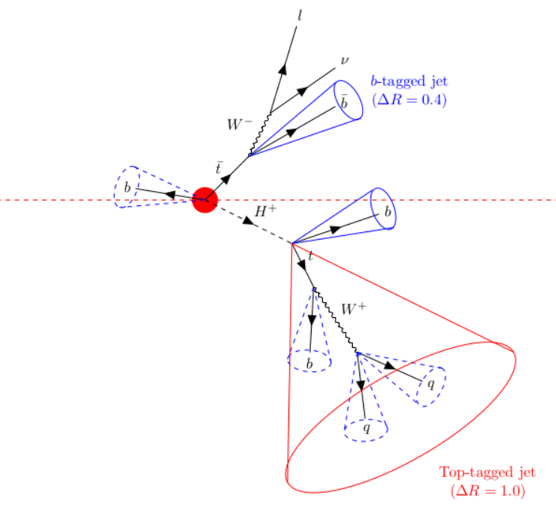
\includegraphics[keepaspectratio,scale=0.8]{images/AnalysisStrategy/EventTopology.png}
  \caption{Schematic of boosted event topology. Signal event has one $J_{\text{top-tag}}$ and at least two $b$-tagged small-$R$ jets.}
  \label{fig:EventTopology_Htb}
\end{figure}
%---

%--- Table of SR1 Event Selections
\begin{table}[H]
  \centering
  \begin{tabular*}{160mm}{l|ll|l}
    \hline\hline
    Cut                       & SR                                                          &                           & CR\\
    \hline
    leptons                   &  - $\text{N}_{\text{lepton}}=1$                             &                           & \\
                              & \underline{Electron}                                        & \underline{Muon}          & Same as SR\\
                              &  - $p_{\text{T}}>27$ GeV                                    &  - $p_{\text{T}}>27$ GeV  & \\
                              &  - $|\eta|<1.37$ or $1.52<|\eta|<2.47$                      &  - $|\eta|<2.5$           & \\
    \hline
    Top-tagged large-$R$ jets &  - $\text{N}_{J_{\text{top-tag}}} \geq 1$                   &                           &\\
                              &  - $350~\text{GeV}<p_{\text{T}}<2500~\text{GeV}$            &                           & Same as SR\\
                              &  - $m>40\text{GeV}$                                         &                           & \\
    \hline
    Small-$R$ jets            &  - $\text{N}_{\text{jet}} \geq 2$                           &                           & $\text{N}_{\text{jet}} \geq 1$ \\
                              &  - $p_{\text{T}}>25$ GeV                                    &                           & (Kinematic requirements\\
                              &  - $|\eta|<2.5$                                             &                           &  are same as SR)\\
                              &  - ${\Delta}R(J_{\text{top-tag}}^{1st}, jet)>1.0$           &                           & \\
    \hline
    $b$-tagged small-$R$ jets & $\text{N}_{b-\text{jet}} \geq 2$                            &                        & $\text{N}_{b-\text{jet}}=1$\\

    \hline\hline
  \end{tabular*}
  \caption{Event selections in the SR and CR. After these selections, the SR becomes enriched in $t\bar{t}+\text{HF}$, and the CR becomes enriched in $t\bar{t}+\text{light}$}
  \label{tab:EventSelectionInSR1AndSR2}
\end{table}

%--- Figure for SR1
\begin{figure}[H]
  \centering
  \subfloat[]{
    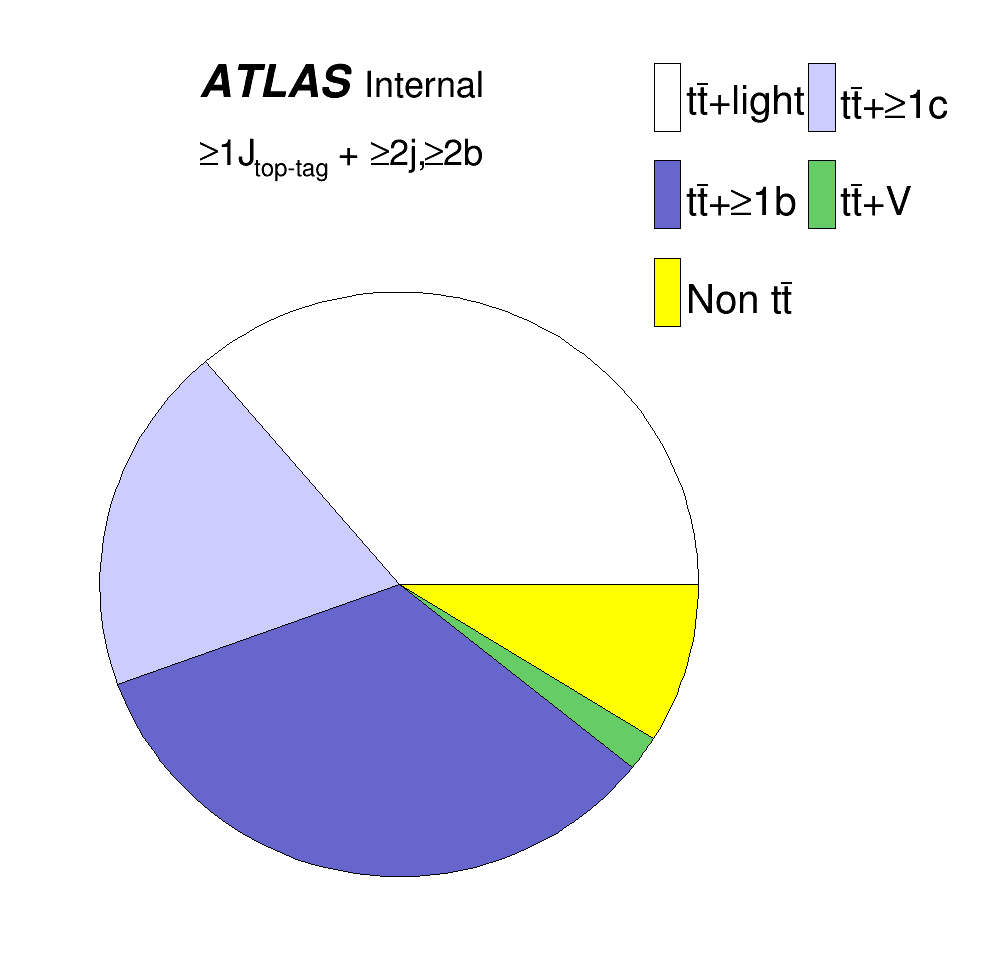
\includegraphics[keepaspectratio,scale=0.2]{images/AnalysisStrategy/PieChart_SR_MVA.png}
    \label{fig:PieChart_SR}
  }
  \subfloat[]{
    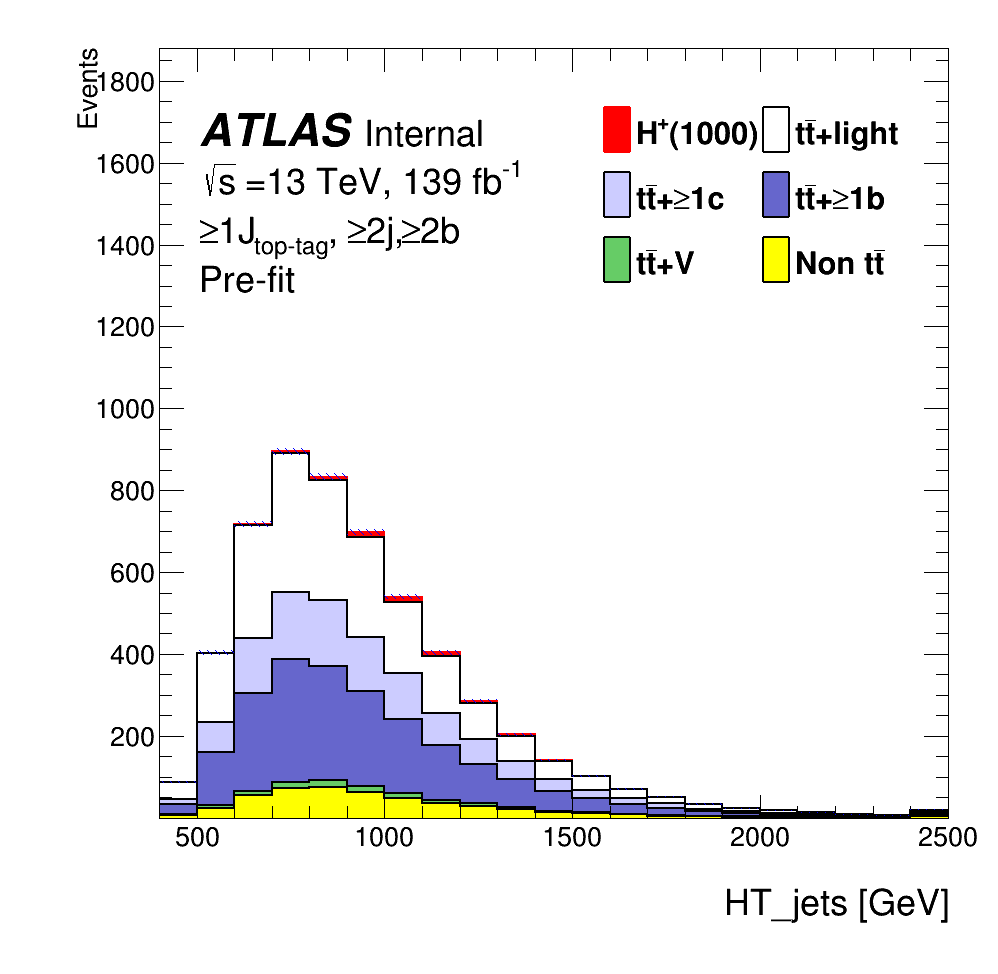
\includegraphics[keepaspectratio,scale=0.2]{images/AnalysisStrategy/HT_jets_SR_MVA.png}
    \label{fig:PieChart_SR1}
  }
  \caption{Background composition in the SR is shown in the pie chart (a) and the $H_{\text{T}}^{\text{jets}}$ distributions (b).}
  \label{fig:BkgComposition_SR1}
\end{figure}


%--- Figure for SR2
\begin{figure}[H]
  \centering
  \subfloat[]{
    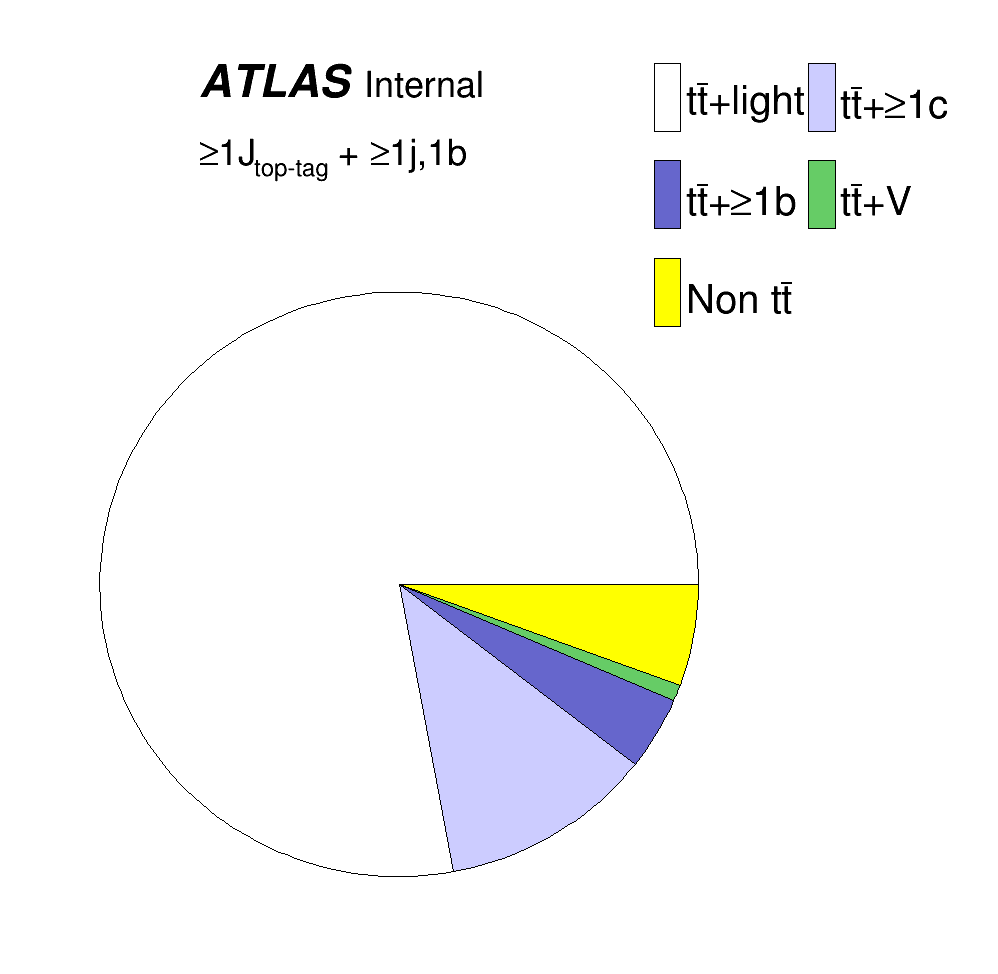
\includegraphics[keepaspectratio,scale=0.2]{images/AnalysisStrategy/PieChart_CR_MVA.png}
    \label{fig:PieChart_SR}
  }
  \subfloat[]{
    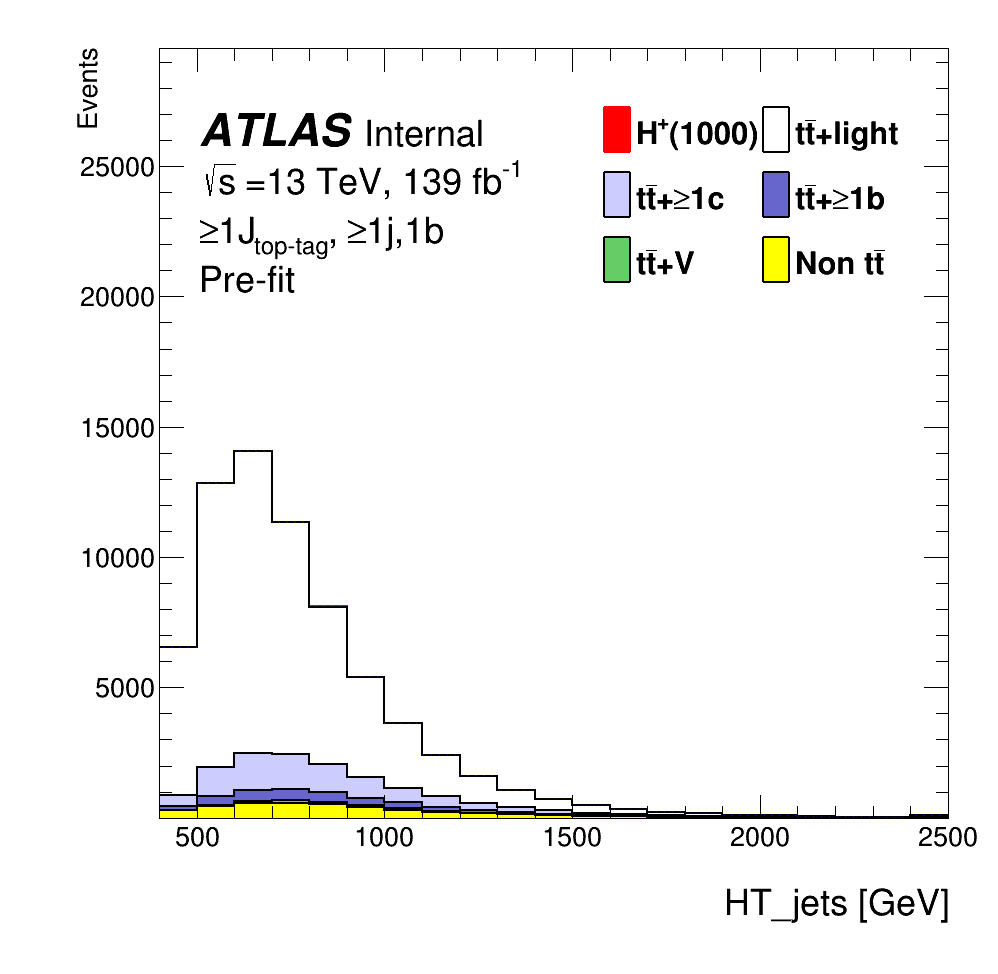
\includegraphics[keepaspectratio,scale=0.2]{images/AnalysisStrategy/HT_jets_CR_MVA.png}
    \label{fig:PieChart_SR1}
  }
  \caption{Background composition in the CR is shown in the pie chart (a) and the $H_{\text{T}}^{\text{jets}}$ distributions (b).}
  \label{fig:BkgComposition_SR2}
\end{figure}

The expected number of signal and background events in the SR and CR are shown in Table \ref{tab:PrefitYields}. For the predicted number of $H^{+}$ signal events with the 1000 and 3000 GeV mass hypothesis, the cross-section of ${\sigma}(pp{\rightarrow}tbH^{+}){\times}Br(H^{+}{\rightarrow}tb)=0.046$ pb is assumed. This corresponds to the upper limit at $M_{H^{+}}=1000$ GeV obtained from the resolved analysis \cite{HDBS-2021-02}. As discussed later in Section \ref{subsec:BlindStrategy}, we use the signal ${\sigma}{\times}Br$ to define the blinded regions. Table \ref{tab:CutflowForSignals} shows the cut flow for each signal sample.

\begin{table}[H]
  \centering
  \begin{tabular*}{120mm}{@{\extracolsep{\fill}}cll}
    \hline\hline
                            & \multicolumn{1}{c}{SR} & \multicolumn{1}{c}{CR}\\
    \hline
    $t\bar{t}+\text{light}$ & $1990\pm  95$           & $ 54008\pm 2667$ \\
    $t\bar{t}+\geq1c$       & $1063\pm 925$           & $  8011\pm 1450$ \\
    $t\bar{t}+\geq1b$       & $1853\pm 931$           & $  2793\pm 1402$ \\
    $t\bar{t}+W$            & $  38\pm   6$           & $   312\pm   41$ \\
    $t\bar{t}+Z$            & $  67\pm  11$           & $   294\pm   38$ \\
    $Wt$ channel            & $ 184\pm 107$           & $  1995\pm  742$ \\
    $t$ channel             & $  37\pm  27$           & $   172\pm   56$ \\
    Other top sources       & $   8\pm   1$           & $    34\pm    5$ \\
    $VV$, $V$+jets          & $ 152\pm  55$           & $  1529\pm  530$ \\
    $t\bar{t}H$             & $ 103\pm   4$           & $   176\pm    5$ \\
    \hline
    Total                   & $5497\pm 270$           & $ 69324\pm 3338$ \\
    \hline
    $H^{+}$ 1000 GeV        & $  56\pm  5$           & $     56\pm   10$ \\
    $H^{+}$ 3000 GeV        & $  72\pm 17$           & $     96\pm   23$ \\
    \hline\hline
  \end{tabular*}
  \caption{Number of expected events in each analysis region. The quoted uncertainties include both statistical and systematic uncertainties before fitting.}
  \label{tab:PrefitYields}
\end{table}

\begin{table}[H]
    \subfloat[] {
    \scalebox{0.70}{
    \begin{tabular*}{250mm}{@{\extracolsep{\fill}}c|cccccccccccccc}
        \hline\hline
        Mass &                        & Gen    & Reco   & TrigDec & 1$\ell$ & TrigMatch & $\geq{1J}$ & $\geq1j$ & $\geq1b^{85}$ & $\geq1J_{\text{non el}}$ & $\geq1J_{\text{top-tag}}$ & $\geq1j_{\text{add}}$ & $\geq1b^{70}_{\text{add}}$ & $\geq2b^{70}_{\text{add}}$\\
         %Mass & Cut1 & Cut2 & Cut3 & Cut4 & CUt5 & Cut6 & Cut7 & Cut8 & Cut9 & Cut10 & Cut11 & Cut12 & Cut13\\
        \hline
        1000 & $\text{N}_{\text{MC}}$ & 998000 & 541248 & 529780  & 342999  & 337300    & 256596     & 256595   & 254364        & 225152                   & 38298                     & 38259                 & 32751       
                                    & 15801\\
             & Cut eff.               & -      & 0.542  & 0.979   & 0.647   & 0.983     & 0.761      & 1.000    & 0.991         & 0.885                    & 0.170                     & 0.999                 & 0.856       
                                    & 0.482\\
        \hline
        1200 & $\text{N}_{\text{MC}}$ & 985000 & 544241 & 534601  & 335452  & 329187    & 269093     & 269093   & 266707        & 237410                   & 48012                     & 47968                 & 40768       
                                    & 19536\\
             & Cut eff.               & -      & 0.553  & 0.982   & 0.627   & 0.981     & 0.817      & 1.000    & 0.991         & 0.890                    & 0.202                     & 0.999                 & 0.850       
                                    & 0.479\\
        \hline
        1400 & $\text{N}_{\text{MC}}$ & 999000 & 560829 & 551672  & 335009  & 328190    & 280389     & 280389   & 277776        & 249152                   & 54672                     & 54626                 & 45817       
                                    & 21893\\
             & Cut eff.               & -      & 0.561  & 0.984   & 0.607   & 0.980     & 0.854      & 1.000    & 0.991         & 0.897                    & 0.219                     & 0.999                 & 0.839       
                                    & 0.478\\ 
        \hline
        1600 & $\text{N}_{\text{MC}}$ & 997000 & 565351 & 556595  & 328781  & 321427    & 282873     & 282873   & 280064        & 253245                   & 58398                     & 58374                 & 48659       
                                    & 23140\\
             & Cut eff.               & -      & 0.567  & 0.985   & 0.591   & 0.978     & 0.880      & 1.000    & 0.990         & 0.904                    & 0.231                     & 1.000                 & 0.834       
                                    & 0.476\\
        \hline
        1800 & $\text{N}_{\text{MC}}$ & 978000 & 559240 & 550740  & 315454  & 307841    & 277151     & 277151   & 273951        & 250241                   & 59500                     & 59468                 & 49081       
                                    & 22671\\
             & Cut eff.               & -      & 0.572  & 0.985   & 0.573   & 0.976     & 0.900      & 1.000    & 0.988         & 0.913                    & 0.238                     & 0.999                 & 0.825       
                                    & 0.462\\
        \hline
        2000 & $\text{N}_{\text{MC}}$ & 996000 & 570655 & 562595  & 312270  & 304274    & 278522     & 278522   & 274935        & 253344                   & 62084                     & 62056                 & 50375       
                                    & 23076\\
             & Cut eff.               & -      & 0.573  & 0.986   & 0.555   & 0.974     & 0.915      & 1.000    & 0.987         & 0.921                    & 0.245                     & 1.000                 & 0.812       
                                    & 0.458\\
        \hline
        2500 & $\text{N}_{\text{MC}}$ & 999000 & 574372 & 566804  & 294566  & 286030    & 268297     & 268297   & 263948        & 248193                   & 64809                     & 64780                 & 51192                                     & 22231\\
             & Cut eff.               & -      & 0.575  & 0.987   & 0.520   & 0.971     & 0.938      & 1.000    & 0.984         & 0.940                    & 0.261                     & 1.000                 & 0.790                                & 0.434\\
        \hline
        3000 & $\text{N}_{\text{MC}}$ & 999000 & 570796 & 563605  & 277515  & 268587    & 255972     & 255972   & 250995        & 239429                   & 66834                     & 66826                 & 51600                                     & 21345\\
             & Cut eff.               & -      & 0.571  & 0.987   & 0.492   & 0.968     & 0.953      & 1.000    & 0.981         & 0.954                    & 0.279                     & 1.000                 & 0.772         
                                    & 0.413\\         
        \hline\hline
    \end{tabular*}
    \label{tab:CutflowForHp}
    }
    }\par
\end{table}

\begin{table}[H]
    \subfloat[]{
    \scalebox{0.70}{
    \begin{tabular*}{250mm}{@{\extracolsep{\fill}}c|cccccccccccccc}
        \hline\hline
        Mass &                        & Gen    & Reco   & TrigDec & 1$\ell$ & TrigMatch & $\geq{1J}$ & $\geq1j$ & $\geq1b^{85}$ & $\geq1J_{\text{non el}}$ & $\geq1J_{\text{top-tag}}$ & $\geq1j_{\text{add}}$ & $\geq1b^{70}_{\text{add}}$ & $\geq2b^{70}_{\text{add}}$\\
        \hline
        1000 & $\text{N}_{\text{MC}}$ & 498000 & 248196 & 241900  & 151833  & 148932    & 118640     & 118640   & 117932        & 107739                   & 18538                     & 18534                 & 16264                                    & 8623\\
             & Cut eff.               & -      & 0.498  & 0.975   & 0.628   & 0.981     & 0.797      & 1.000    & 0.994         & 0.914                    & 0.172                     & 1.000                 & 0.878                               & 0.530\\
        \hline
        1200 & $\text{N}_{\text{MC}}$ & 497000 & 254395 & 248661  & 152134  & 148969    & 125935     & 125935   & 125170        & 114663                   & 22658                     & 22653                 & 19664         
                                   & 10291\\
             & Cut eff.               & -      & 0.512  & 0.977   & 0.612   & 0.979     & 0.845      & 1.000    & 0.994         & 0.916                    & 0.198                     & 1.000                 & 0.868                               & 0.523\\
        \hline
        1400 & $\text{N}_{\text{MC}}$ & 499000 & 260545 & 255004  & 151933  & 148562    & 130183     & 130183   & 129327        & 118716                   & 24673                     & 24667                 & 21203                                    & 11079\\
             & Cut eff.               & -      & 0.522  & 0.979   & 0.596   & 0.978     & 0.876      & 1.000    & 0.993         & 0.918                    & 0.208                     & 1.000                 & 0.860                               & 0.523\\
        \hline
        1600 & $\text{N}_{\text{MC}}$ & 497000 & 263865 & 258714  & 150482  & 146957    & 131867     & 131867   & 130959        & 121196                   & 26420                     & 26412                 & 22631                                    & 11616\\
             & Cut eff.               & -      & 0.531  & 0.980   & 0.582   & 0.977     & 0.897      & 1.000    & 0.993         & 0.925                    & 0.218                     & 1.000                 & 0.857                               & 0.513\\
        \hline
        1800 & $\text{N}_{\text{MC}}$ & 490000 & 263070 & 258072  & 145536  & 141752    & 129382     & 129382   & 128408        & 119539                   & 27016                     & 27014                 & 22925                                    & 11728\\
             & Cut eff.               & -      & 0.537  & 0.981   & 0.564   & 0.974     & 0.913      & 1.000    & 0.992         & 0.931                    & 0.226                     & 1.000                 & 0.849                               & 0.512\\
        \hline
        2000 & $\text{N}_{\text{MC}}$ & 500000 & 269918 & 265056  & 145830  & 141828    & 131486     & 131486   & 130372        & 122004                   & 28059                     & 28053                 & 23583                                    & 11914\\
             & Cut eff.               & -      & 0.540  & 0.982   & 0.550   & 0.973     & 0.927      & 1.000    & 0.992         & 0.936                    & 0.230                     & 1.000                 & 0.841         
                                   & 0.505\\
        \hline
        2500 & $\text{N}_{\text{MC}}$ & 497000 & 271566 & 267051  & 137291  & 133192    & 125774     & 125774   & 124454        & 117931                   & 29003                     & 28999                 & 23868                                    & 11596\\
             & Cut eff.               & -      & 0.546  & 0.983   & 0.514   & 0.970     & 0.944      & 1.000    & 0.990         & 0.948                    & 0.246                     & 1.000                 & 0.823                               & 0.486\\
        \hline
        3000 & $\text{N}_{\text{MC}}$ & 489000 & 267310 & 262927  & 126289  & 121989    & 116513     & 116513   & 115007        & 109992                   & 28753                     & 28750                 & 23174                                    & 10622\\
             & Cut eff.               & -      & 0.547  & 0.984   & 0.480   & 0.966     & 0.955      & 1.000    & 0.987         & 0.956                    & 0.261                     & 1.000                 & 0.806         
                                   & 0.458\\ 
        \hline\hline
    \end{tabular*}
    \label{tab:CutflowForWpLH}
    }
    }\par

    \subfloat[]{
    \scalebox{0.70}{
    \begin{tabular*}{250mm}{@{\extracolsep{\fill}}c|cccccccccccccc}
        \hline\hline
        Mass &                        & Gen    & Reco   & TrigDec & 1$\ell$ & TrigMatch & $\geq{1J}$ & $\geq1j$ & $\geq1b^{85}$ & $\geq1J_{\text{non el}}$ & $\geq1J_{\text{top-tag}}$ & $\geq1j_{\text{add}}$ & $\geq1b^{70}_{\text{add}}$ & $\geq2b^{70}_{\text{add}}$\\
        \hline
        1000 & $\text{N}_{\text{MC}}$ & 499000 & 294866 & 290492  & 186576  & 183583    & 147606     & 147606   & 146329        & 131251                   & 24304                     & 24293                 & 21011                                    & 10895\\
             & Cut eff.               & -      & 0.591  & 0.985   & 0.642   & 0.984     & 0.804      & 1.000    & 0.991         & 0.897                    & 0.185                     & 1.000                 & 0.865                               & 0.519\\
        \hline
        1200 & $\text{N}_{\text{MC}}$ & 500000 & 300323 & 296365  & 185318  & 181937    & 154413     & 154413   & 153000        & 138404                   & 29012                     & 28997                 & 24801                                    & 12811\\
             & Cut eff.               & -      & 0.601  & 0.987   & 0.625   & 0.982     & 0.849      & 1.000    & 0.991         & 0.905                    & 0.210                     & 1.000                 & 0.855         
                                   & 0.517\\
        \hline
        1400 & $\text{N}_{\text{MC}}$ & 500000 & 303573 & 299866  & 181675  & 178152    & 156905     & 156905   & 155480        & 141630                   & 32480                     & 32470                 & 27571                                    & 13870\\
             & Cut eff.               & -      & 0.607  & 0.988   & 0.606   & 0.981     & 0.881      & 1.000    & 0.991         & 0.911                    & 0.229                     & 1.000                 & 0.849         
                                   & 0.503\\
        \hline
        1600 & $\text{N}_{\text{MC}}$ & 498000 & 304438 & 300981  & 177434  & 173574    & 156104     & 156104   & 154405        & 141953                   & 34356                     & 34336                 & 28999                                    & 14487\\
             & Cut eff.               & -      & 0.611  & 0.989   & 0.590   & 0.978     & 0.899      & 1.000    & 0.989         & 0.919                    & 0.242                     & 0.999                 & 0.845                               & 0.500\\
        \hline
        1800 & $\text{N}_{\text{MC}}$ & 488000 & 299636 & 296508  & 170489  & 166656    & 152480     & 152480   & 150711        & 139586                   & 34423                     & 34413                 & 28710                                    & 14220\\
             & Cut eff.               & -      & 0.614  & 0.990   & 0.575   & 0.978     & 0.915      & 1.000    & 0.988         & 0.926                    & 0.247                     & 1.000                 & 0.834                               & 0.495\\
        \hline
        2000 & $\text{N}_{\text{MC}}$ & 488000 & 300376 & 297075  & 166140  & 162131    & 150247     & 150247   & 148297        & 138313                   & 35279                     & 35265                 & 29166                                    & 14182\\
             & Cut eff.               & -      & 0.616  & 0.989   & 0.559   & 0.976     & 0.927      & 1.000    & 0.987         & 0.933                    & 0.255                     & 1.000                 & 0.827                               & 0.486\\
        \hline
        2500 & $\text{N}_{\text{MC}}$ & 498000 & 305572 & 302770  & 159971  & 155580    & 146930     & 146930   & 144597        & 136696                   & 36850                     & 36841                 & 29578                                    & 13558\\
             & Cut eff.               & -      & 0.614  & 0.991   & 0.528   & 0.973     & 0.944      & 1.000    & 0.984         & 0.945                    & 0.270                     & 1.000                 & 0.802         
                                   & 0.458\\
        \hline
        3000 & $\text{N}_{\text{MC}}$ & 499000 & 304217 & 301493  & 152213  & 147658    & 140988     & 140988   & 138344        & 132052                   & 37948                     & 37944                 & 29674                                    & 13047\\
             & Cut eff.               & -      & 0.610  & 0.991   & 0.504   & 0.970     & 0.955      & 1.000    & 0.981         & 0.955                    & 0.287                     & 1.000                 & 0.782                               & 0.440\\
        \hline\hline
    \end{tabular*}
    \label{tab:CutflowForWpRH}
    }
    }
    \caption{Cut flow for the $H^{+}$ (a), $W'_{\text{LH}}$ (b), and $W'_{\text{RH}}$ (c) signal: for each sample the corresponding mass, the number of generated events (Gen), the number of reconstructed events (Reco), the number of events that pass lepton triggers (TrigDec), the number of events that have an electron or muon with $p_{\text{T}}$ larger than 27 GeV ($1\ell$), the number of events that the lepton matches to the one detected with the trigger (TrigMatch), the number of events that have at least one large-R jets with $p_{\text{T}}$ larger than 200 GeV ($\geq1J$), the number of events that have at least one small-R jets with $p_{\text{T}}$ larger than 25 GeV ($\geq1j$), the number of events that have at least one $b$-tagged jets at the 85\% efficiency working point ($\geq1b^{85}$), the number of events that have at least one large-R jets with ${\Delta}R$ to the electron smaller than 1.0 ($\geq1J_{\text{non el}}$), the number of events that have at least one top-tagged large-R jets with contained top-tagger at the 80\% efficiency working point ($\geq1J_{\text{top-tag}}$), the number of events that have at least additional small-R jets with ${\Delta}R$ to the leading top-tagged large-R jet larger than 1.0 ($\geq1j_{\text{add}}$), the number of events that have at least one or two $b$-tagged additional small-R jets at the 70\% efficiency working point ($\geq1b^{70}$, $\geq2b^{70}$ ) are shown in the top rows ($\text{N}_{\text{MC}}$). Each cut efficiency is also shown in the bottom rows (Cut eff.).}
    \label{tab:CutflowForSignals}
\end{table}


\subsubsection{Multivariable analysis using BDT}
\label{subsubsec:MVA}

In this search, the most important background is $t\bar{t}+\text{jets}$ as discussed in Section \ref{subsec:AnaStrategyUnder3TeV}. To enhance the separation between signal and background, multivariable analysis is performed using Boosted Decision Trees (BDT) technique of TMVA \cite{TMVA}. Obtained BDT score distribution is used in the profile likelihood fit as a final discriminant (Section \ref{sec:ProfileLikelohoodFit}).

\begin{description}
    \item{\textbf{Signal and background definition in BDT training}}\mbox{}\\
    To classify signal ($H^{+}$ and $W'$) and $t\bar{t}+\text{jets}$ background events, BDTs are trained using the simulated $H^{+}$ signal and $t\bar{t}+\text{jets}$ background samples. This analysis under 3 TeV mass points considers eight different mass hypotheses, and the training is performed on each mass hypothesis. On the other hand, the $t\bar{t}+\text{jets}$ background samples are common in each training. Since kinematics of $H^+$ signals become harder in higher mass hypotheses, the BDTs trained using the higher $H^{+}$ mass samples typically have greater separation power. These signal events and background events used in training are required to pass either SR criteria. These BDTs optimized using $H^{+}$ signal samples can be also used in $W' \rightarrow tb$ analysis because the difference between a $H^{+}$ and $W'$ is only their spin and the kinematic characteristics of $W' \rightarrow tb$ events are similar to the ones of $H^{+} \rightarrow tb$ events. This validation is done in the section below. BDTs are also trained using 4 and 5 TeV mass point samples. These BDT outputs are only used for the study in Section \ref{subsec:ReweightingTechnique}.

    \item{\textbf{BDT training settings}}\mbox{}\\
    To fully use the simulation samples' statistics, we adopt the 4-fold cross-validation method in the BDT training (Figure \ref{fig:CrossValidationScheme}). Each simulation sample is divided into four sub-datasets (Fold1, Fold2, Fold3, and Fold4). For each MC event, a random number is generated with the MC event number as a seed, and the event is categorized into one of the sub-datasets according to the generated number. Two of the four sub-datasets are labelled "TRAIN," which are used for BDT training. One of the other sub-datasets is labelled "VALID" and is used to optimize the BDT performance. The last sample, "TEST", is used to construct a fit template. Four combinations of sub-dataset usage (Split1 to Split4 in Figure \ref{fig:CrossValidationScheme}) are tried, and we obtain four statistically-independent BDTs and fit templates. They are combined into one fit template used in the profile likelihood fit (Section.\ref{sec:ProfileLikelohoodFit}).
    
    \begin{figure}[H]
        \centering
        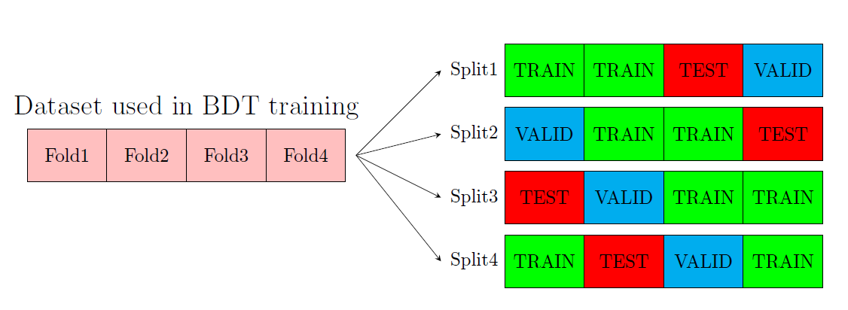
\includegraphics[keepaspectratio,scale=0.65]{images/AnalysisStrategy/CrossValidationScheme.png}
        \caption{Scheme of 4-fold cross-validation of BDT in this analysis.}
        \label{fig:CrossValidationScheme}
    \end{figure}
    
    Hyperparameters for the BDTs are summarized in Table. \ref{tab:Hyperparameters}. Those hyperparameters are chosen to obtain the best sensitivity.

    \begin{table}[H]
      \centering
      \begin{tabular*}{75mm}{@{\extracolsep{\fill}}ll}
        \hline
        \multicolumn{1}{c}{Configuration} & \multicolumn{1}{c}{}\\
        \hline\hline
        \multicolumn{1}{l}{Algorithm}     & \multicolumn{1}{c}{Gradient boosting}\\
        \hline
        $Hyperparameters$ & \\
        \multicolumn{1}{l}{NTrees}       & \multicolumn{1}{c}{100}\\
        \multicolumn{1}{l}{MinNodeSize}  & \multicolumn{1}{c}{2.5}\\
        \multicolumn{1}{l}{MaxDepth}     & \multicolumn{1}{c}{3}\\
        \multicolumn{1}{l}{nCuts}        & \multicolumn{1}{c}{20}\\
        \hline
      \end{tabular*}
      \caption{List of hyperparameters used in the training of a BDT}
      \label{tab:Hyperparameters}
    \end{table}

    \item{\textbf{Input variables in BDT}}\mbox{}\\
    \label{item:BDTInputVars}
    Jets originating from a $H^{+}$ ($W'$) decay have higher $p_\text{T}$ comparing with $t\bar{t}+\text{jets}$ events due to its heavy mass. Additionally, angular and kinematics correlation among jets are different between $H^{+}$ ($W'$) and $t\bar{t}+\text{jets}$ events because these bosons create a resonance. The BDT is trained to exploit these kinematic characteristics fully. The variables used in BDT training are summarized in Table \ref{tab:BDTInputVariables}. Any variables for missing $E_{T}$ are not used in BDT training. In Figure \ref{fig:SOVERB_Hp3000_Contained80_DL1r_70}, each distribution in the $H^{+}$ sample with a mass of 3000~GeV is compared with the $t\bar{t}+\text{jets}$ background. Table \ref{tab:RankingOfBDTInputVariables_Hp3000} shows the ranking of these variables.

    \begin{table}[H]
      \centering
      \begin{tabular*}{150mm}{@{\extracolsep{\fill}}ll}
        \hline
        \multicolumn{1}{c}{Symbol} & \multicolumn{1}{c}{Description}\\
        \hline\hline
        HT\_jets                                   & Scalar sum of the transverse energy of all jets\\
        LeadingJet\_pt                             & Leading jet $p_\text{T}$\\
        Mjjj\_MaxPt                                & Invariant mass of the jet triplet with maximum $p_\text{T}$\\
        Mbb\_MaxPt                                 & Invariant mass of the b-jet pair with maximum $p_\text{T}$\\
        Muu\_MindR                                 & Invariant mass of the untagged jet-pair with minimum $\Delta{R}$\\
        dRlepbb\_MindR                             & $\Delta{R}$ between the lepton and the pair of $b$-jets with smallest $\Delta{R}$\\
        dRbb\_avg                                  & Average $\Delta{R}$ between all $b$-jet pairs in the event\\
        Centrality\_all                            & Centrality calculated using all jets and leptons\\
        H1\_all                                    & Second Fox-Wolfram moment calculated using all jets and lepton\\
        LeadingTop\_pt                             & Leading top-tagged jet $p_\text{T}$\\
        LeadingTop\_m                              & Invariant mass of leading top-tagged jet \\
        Pt\_tb                                     & $p_\text{T}$ of the pair of leading top-tagged jet and leading $b$-jet\\
        M\_tb                                      & Invariant mass of the pair of leading top-tagged jet and leading $b$-jet\\
        PtAsymm\_tb                                & $p_\text{T}$ asymmetry between leading top-tagged jet and leading $b$-jet\\
        \hline
      \end{tabular*}
      \caption{List of variables included in the training of the BDT}
      \label{tab:BDTInputVariables}
    \end{table}

    %--- Ranking @H+(3000)
    \begin{table}[H]
      \centering
      \begin{tabular*}{160mm}{@{\extracolsep{\fill}}lllllll}
        \hline\hline
        \multirow{2}{*}{Ranking} & \multirow{2}{*}{Variable} & \multicolumn{5}{c}{Importance}\\
                                 &                           & Fold1 & Fold2 & Fold3 & Fold4 & Avg.\\
        \hline
        1  & HT\_jets        & 9.509E-02 & 1.118E-01 & 1.216E-01 & 1.073E-01 & 1.089E-01\\
        2  & Centrality\_all & 1.053E-01 & 9.995E-02 & 1.126E-01 & 1.012E-01 & 1.048E-01\\
        3  & M\_tb           & 9.192E-02 & 9.473E-02 & 8.282E-02 & 8.014E-02 & 8.740E-02\\
        4  & LeadingTop\_pt  & 8.710E-02 & 8.107E-02 & 6.472E-02 & 7.292E-02 & 7.645E-02\\
        5  & Pt\_tb          & 7.944E-02 & 7.816E-02 & 7.888E-02 & 6.795E-02 & 7.611E-02\\
        6  & LeadingJet\_pt  & 6.180E-02 & 7.860E-02 & 6.628E-02 & 7.577E-02 & 7.061E-02\\
        7  & dRlepbb\_MindR  & 6.997E-02 & 7.842E-02 & 6.968E-02 & 6.393E-02 & 7.050E-02\\
        8  & dRbb\_avg       & 6.236E-02 & 6.435E-02 & 5.331E-02 & 7.843E-02 & 6.461E-02\\
        9  & Mbb\_MaxPt      & 5.348E-02 & 6.657E-02 & 7.339E-02 & 5.552E-02 & 6.224E-02\\
        10 & PtAsymm\_tb     & 5.209E-02 & 6.526E-02 & 5.843E-02 & 6.620E-02 & 6.050E-02\\
        11 & Mjjj\_MaxPt     & 6.439E-02 & 6.248E-02 & 5.503E-02 & 5.577E-02 & 5.942E-02\\
        12 & H1\_all         & 6.316E-02 & 4.577E-02 & 4.876E-02 & 6.291E-02 & 5.515E-02\\
        13 & LeadingTop\_m   & 5.868E-02 & 3.864E-02 & 5.567E-02 & 5.748E-02 & 5.262E-02\\
        14 & Muu\_MindR      & 4.438E-02 & 3.422E-02 & 5.889E-02 & 5.439E-02 & 4.797E-02\\
        \hline\hline
      \end{tabular*}
      \caption{Importance ranking of variables used in BDT training on 3000 GeV H+ mass hypothesis. Importance values are output from TMVA.}
      \label{tab:RankingOfBDTInputVariables_Hp3000}
    \end{table}

    \begin{figure}[H]
      \subfloat[HT\_jets] {
        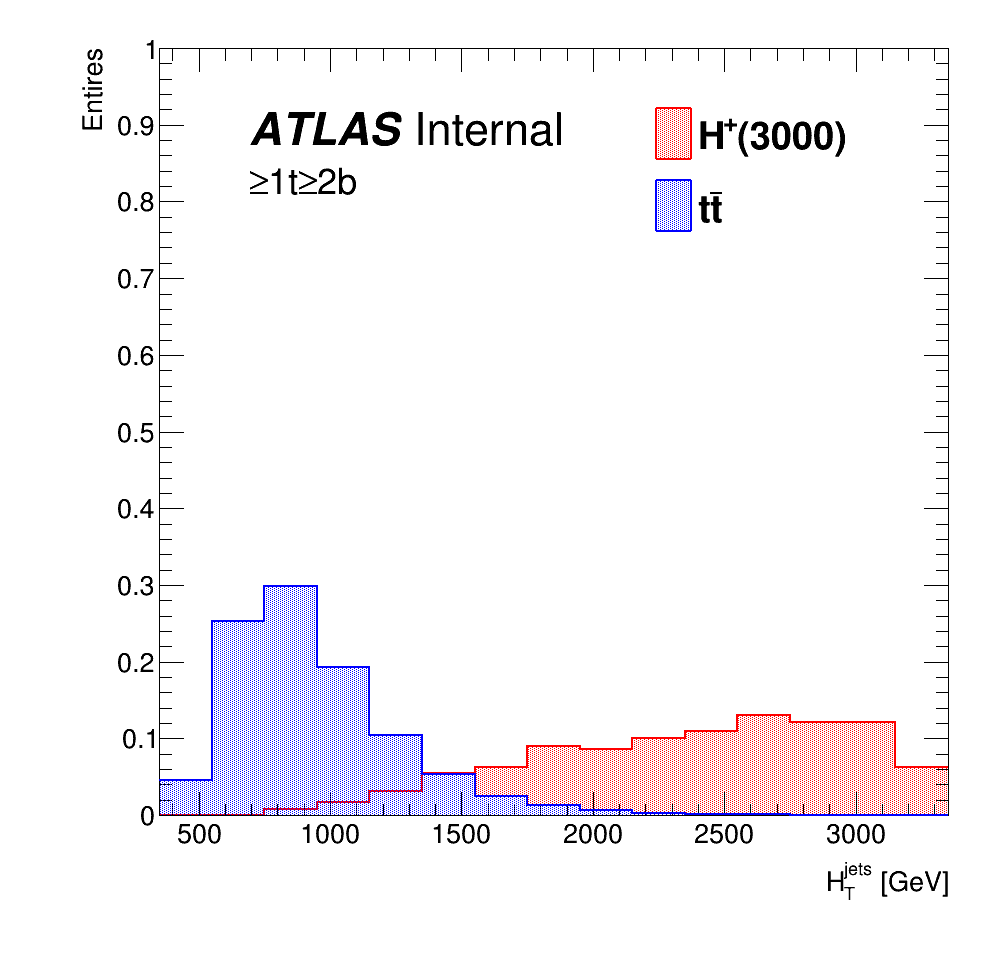
\includegraphics[width=0.25\textwidth]{images/AnalysisStrategy/SOVERB_Hp3000_Contained80_DL1r_70_HT_jets_Contained80_DL1r_70.png}
        \label{fig:SOVERB_HT_jets_Hp3000_Contained80_DL1r_70}
      }
      \subfloat[LeadingJet\_pt] {
        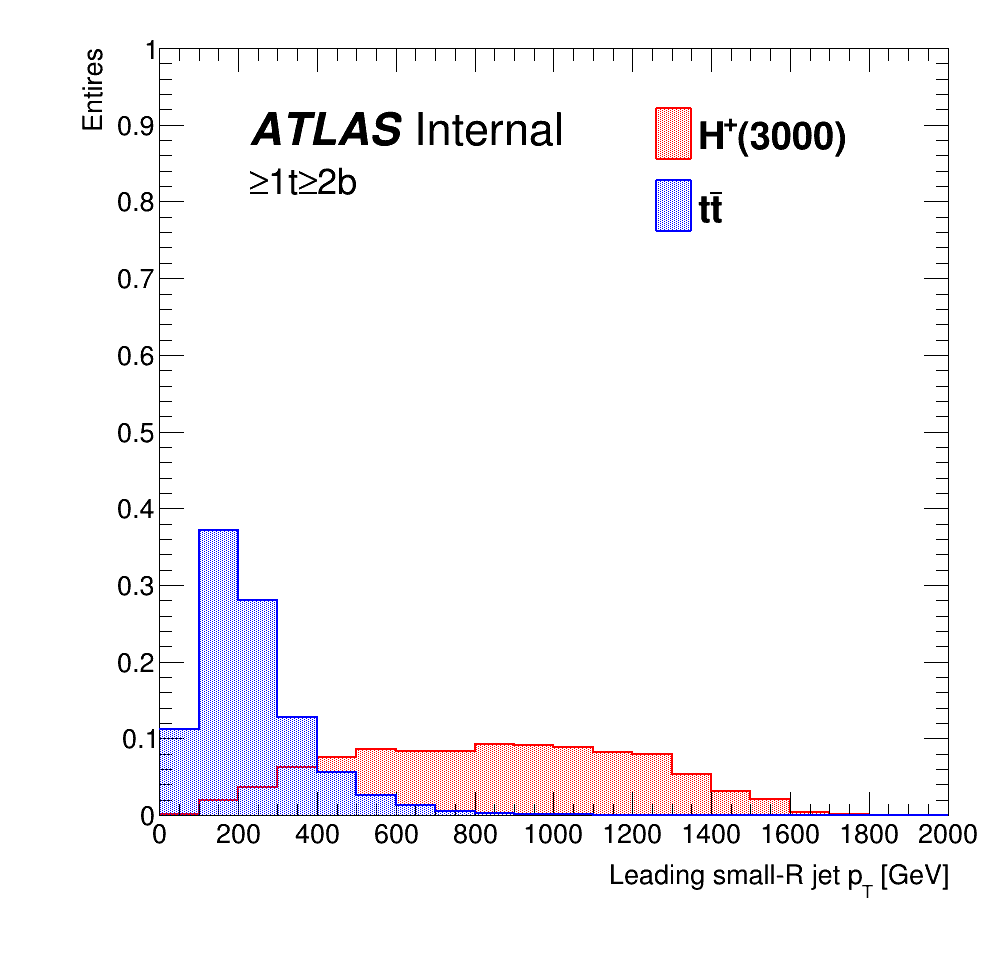
\includegraphics[width=0.25\textwidth]{images/AnalysisStrategy/SOVERB_Hp3000_Contained80_DL1r_70_leadingJet_pt_Contained80_DL1r_70.png}
        \label{fig:SOVERB_LeadingJet_pt_Hp3000_Contained80_DL1r_70}
      }
      \subfloat[Centrality\_all] {
        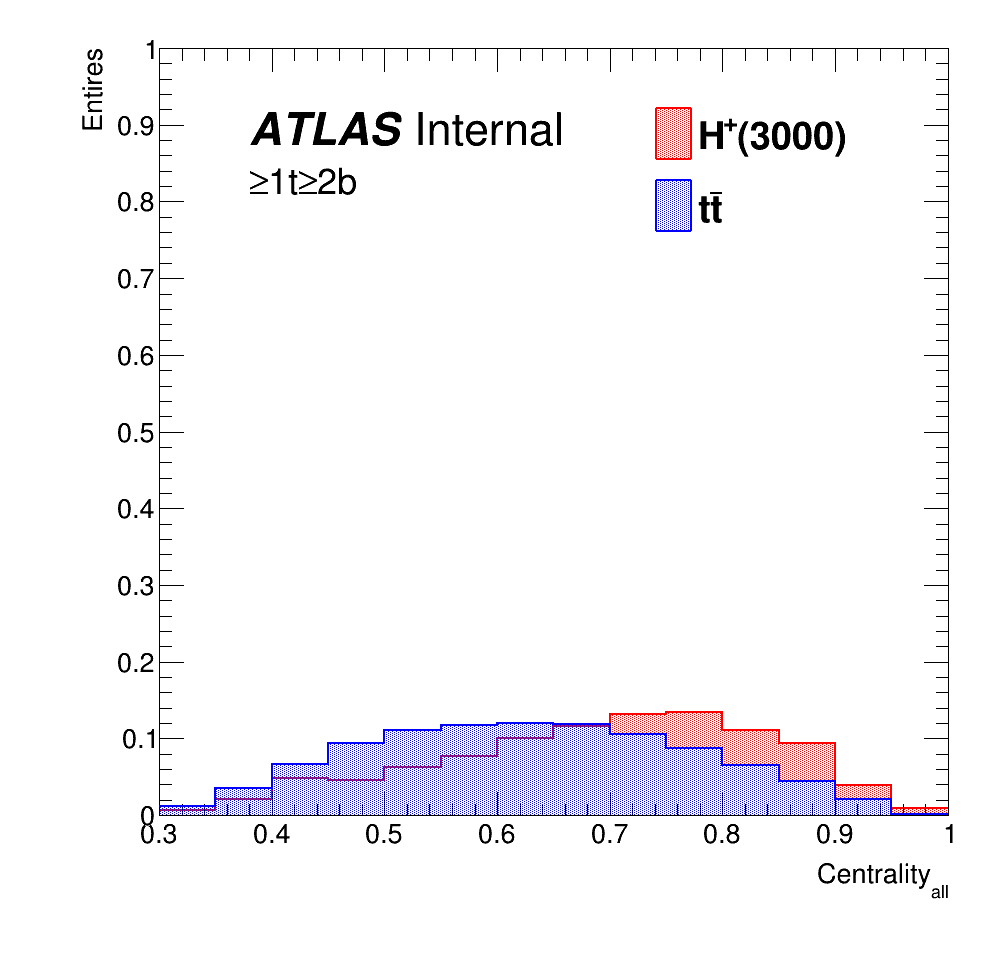
\includegraphics[width=0.25\textwidth]{images/AnalysisStrategy/SOVERB_Hp3000_Contained80_DL1r_70_Centrality_all_Contained80_DL1r_70.png}
        \label{fig:SOVERB_Centrality_all_Hp3000_Contained80_DL1r_70}
      }
      \subfloat[H1\_all] {
        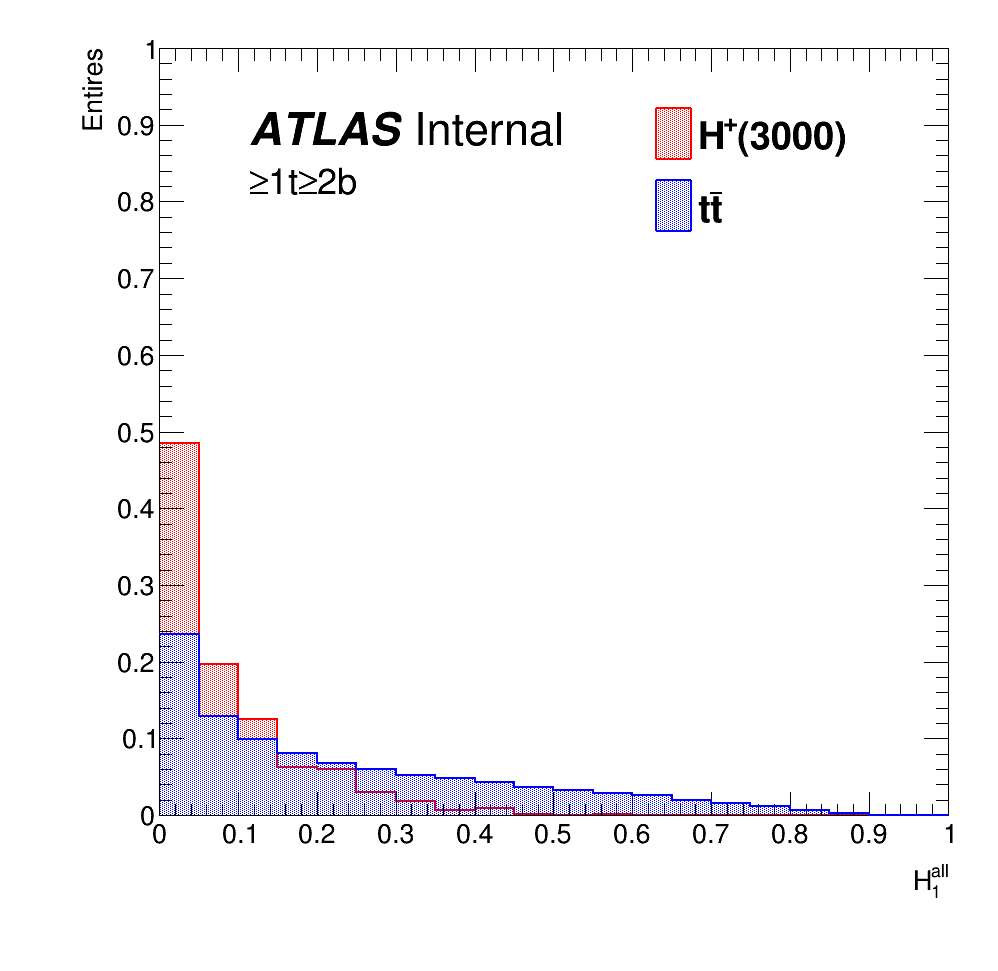
\includegraphics[width=0.25\textwidth]{images/AnalysisStrategy/SOVERB_Hp3000_Contained80_DL1r_70_H1_all_Contained80_DL1r_70.png}
        \label{fig:SOVERB_H1_all_Hp3000_Contained80_DL1r_70}
      }\\
      \subfloat[Mbb\_MaxPt] {
        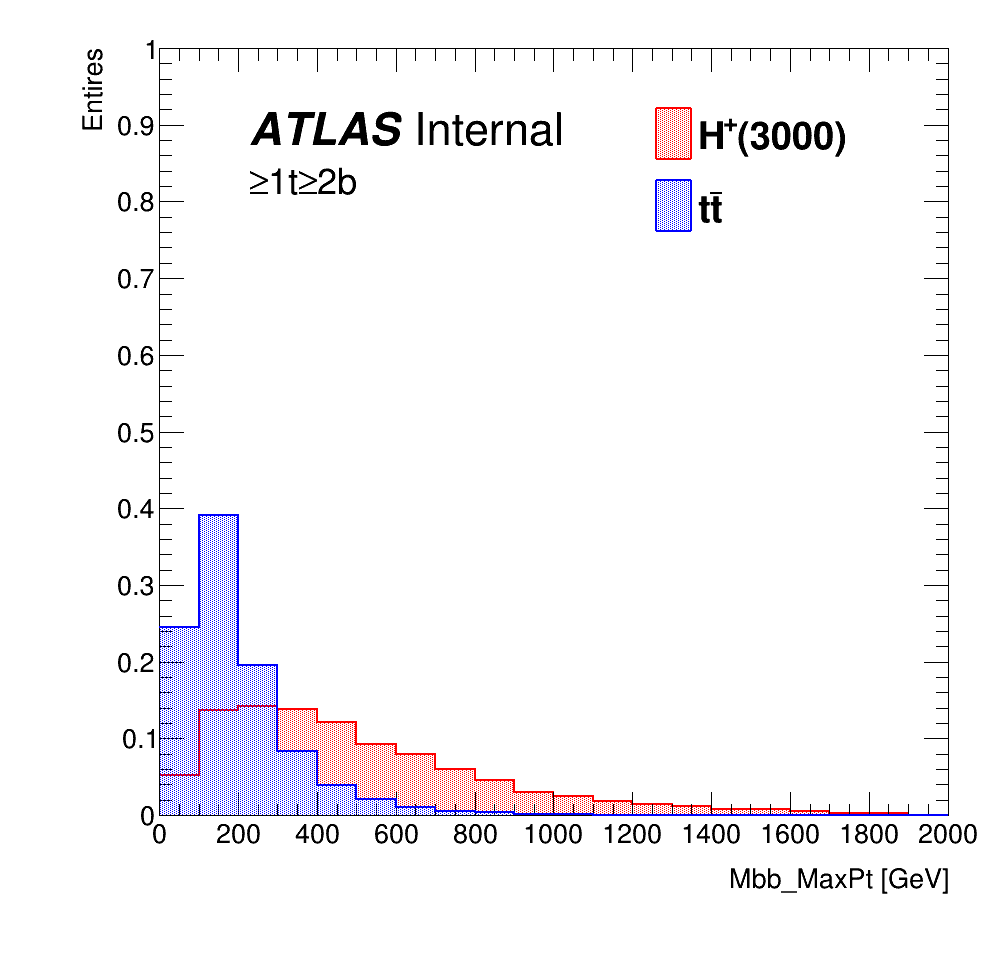
\includegraphics[width=0.25\textwidth]{images/AnalysisStrategy/SOVERB_Hp3000_Contained80_DL1r_70_Mbb_MaxPt_Contained80_DL1r_70.png}
        \label{fig:SOVERB_Mbb_MaxPt_Hp3000_Contained80_DL1r_70}
      }
      \subfloat[Mjjj\_MaxPt] {
        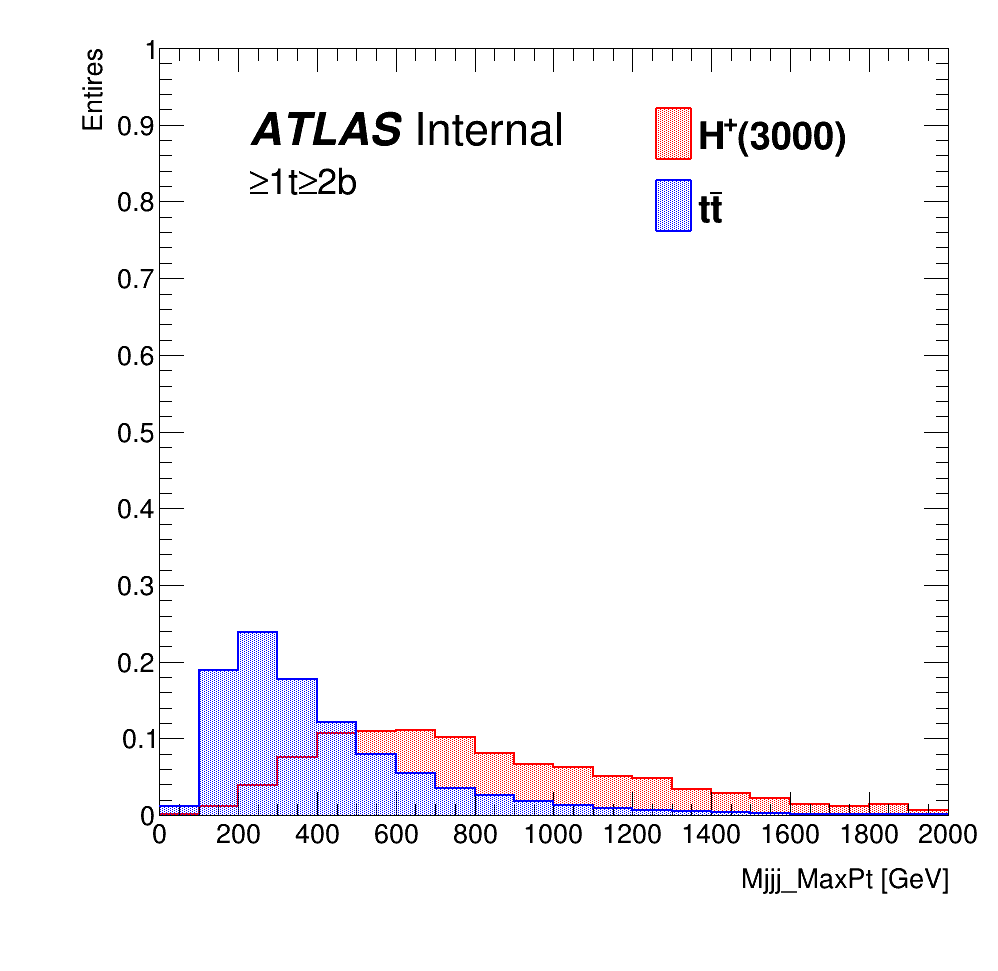
\includegraphics[width=0.25\textwidth]{images/AnalysisStrategy/SOVERB_Hp3000_Contained80_DL1r_70_Mjjj_MaxPt_Contained80_DL1r_70.png}
        \label{fig:SOVERB_Mjjj_MaxPt_Hp3000_Contained80_DL1r_70}
      }
      \subfloat[Muu\_MindR] {
        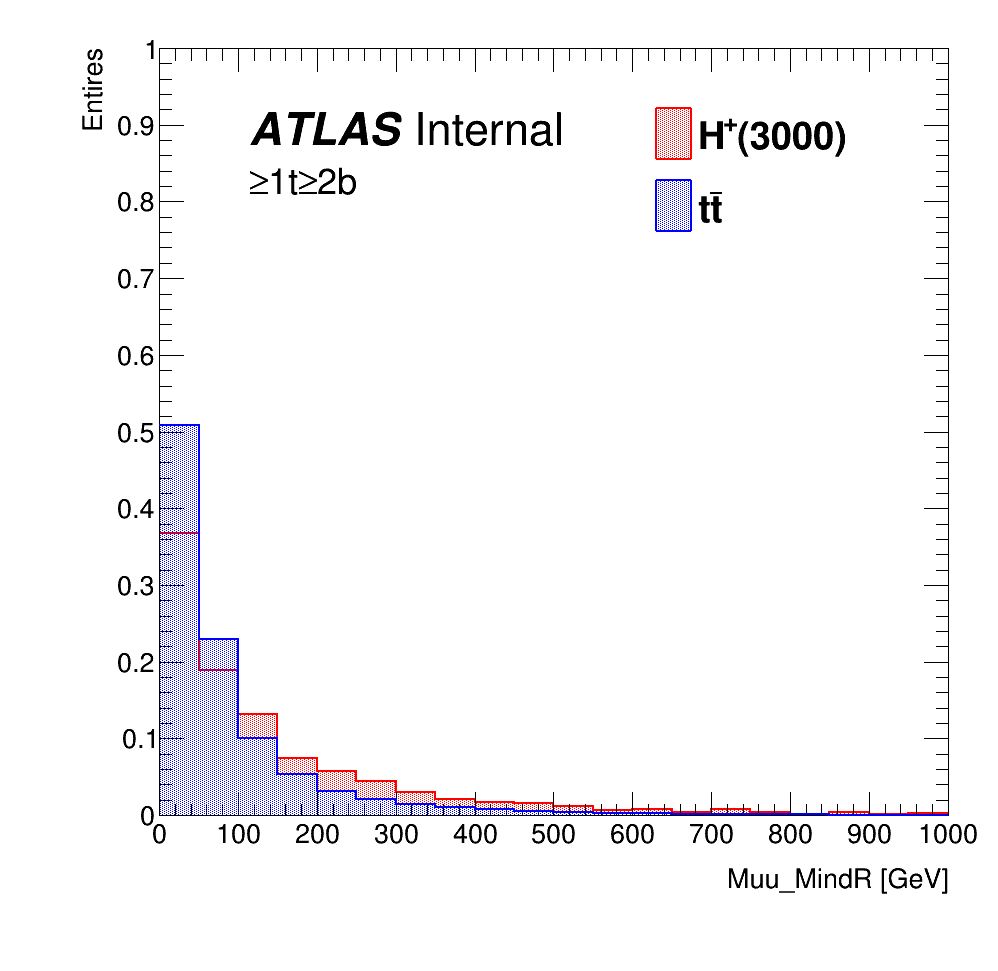
\includegraphics[width=0.25\textwidth]{images/AnalysisStrategy/SOVERB_Hp3000_Contained80_DL1r_70_Muu_MindR_Contained80_DL1r_70.png}
        \label{fig:SOVERB_Muu_MindR_Hp3000_Contained80_DL1r_70}
      }
      \subfloat[dRbb\_avg] {
        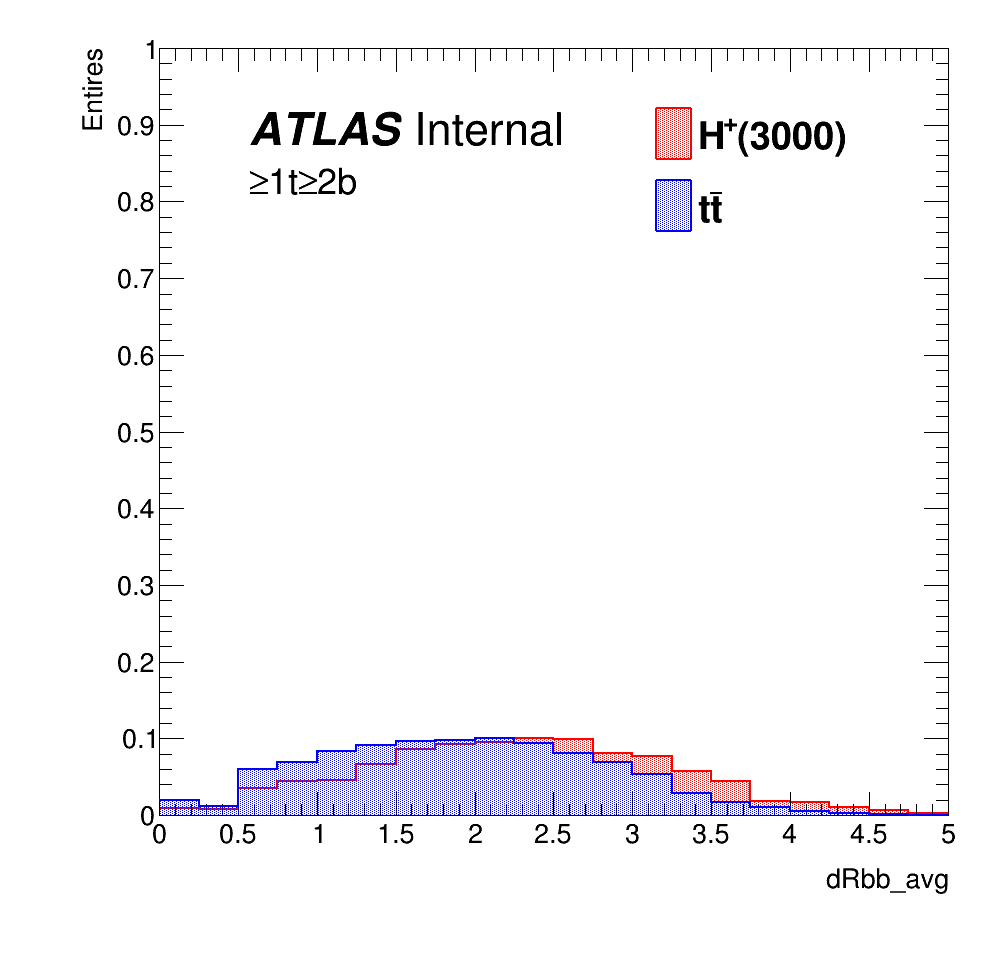
\includegraphics[width=0.25\textwidth]{images/AnalysisStrategy/SOVERB_Hp3000_Contained80_DL1r_70_dRbb_avg_Contained80_DL1r_70.png}
        \label{fig:SOVERB_dRbb_avg_Hp3000_Contained80_DL1r_70}
      }\\
      \subfloat[dRlepbb\_MindR] {
        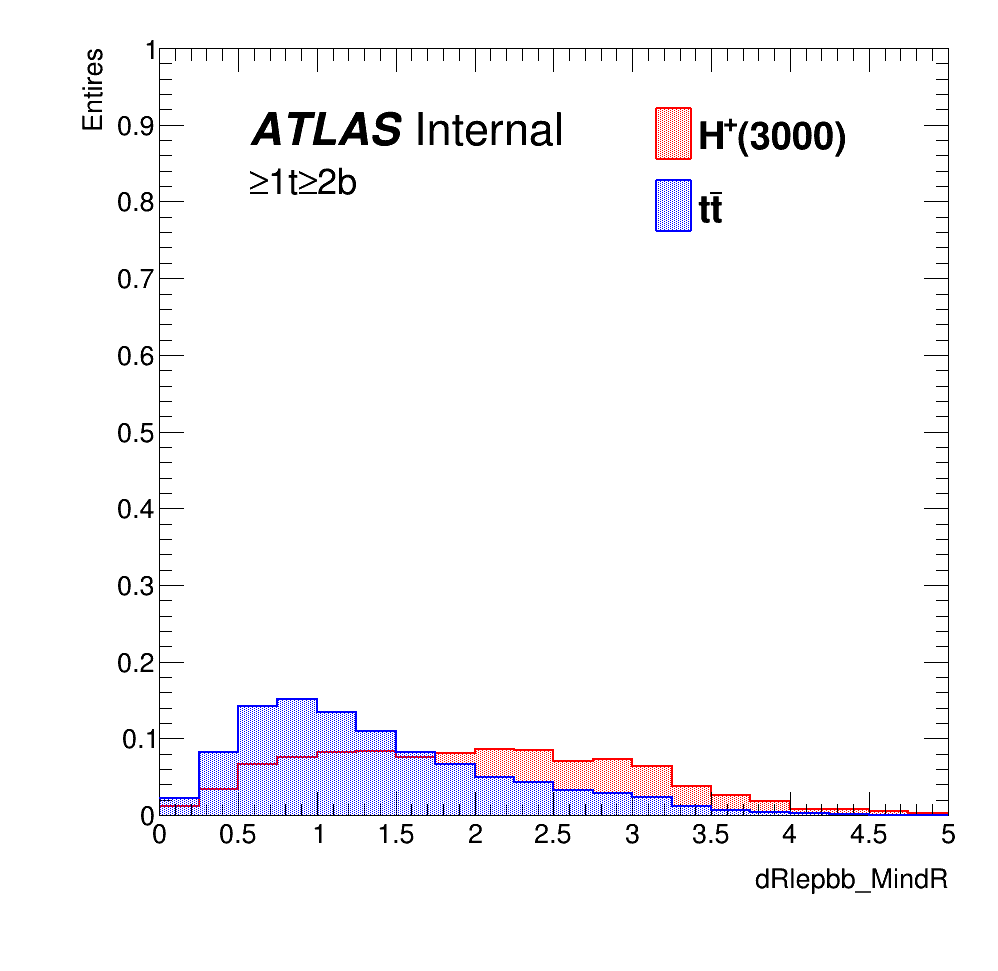
\includegraphics[width=0.25\textwidth]{images/AnalysisStrategy/SOVERB_Hp3000_Contained80_DL1r_70_dRlepbb_MindR_Contained80_DL1r_70.png}
        \label{fig:SOVERB_dRlepbb_MindR_Hp3000_Contained80_DL1r_70}
      }
      \subfloat[LeadingTop\_m] {
        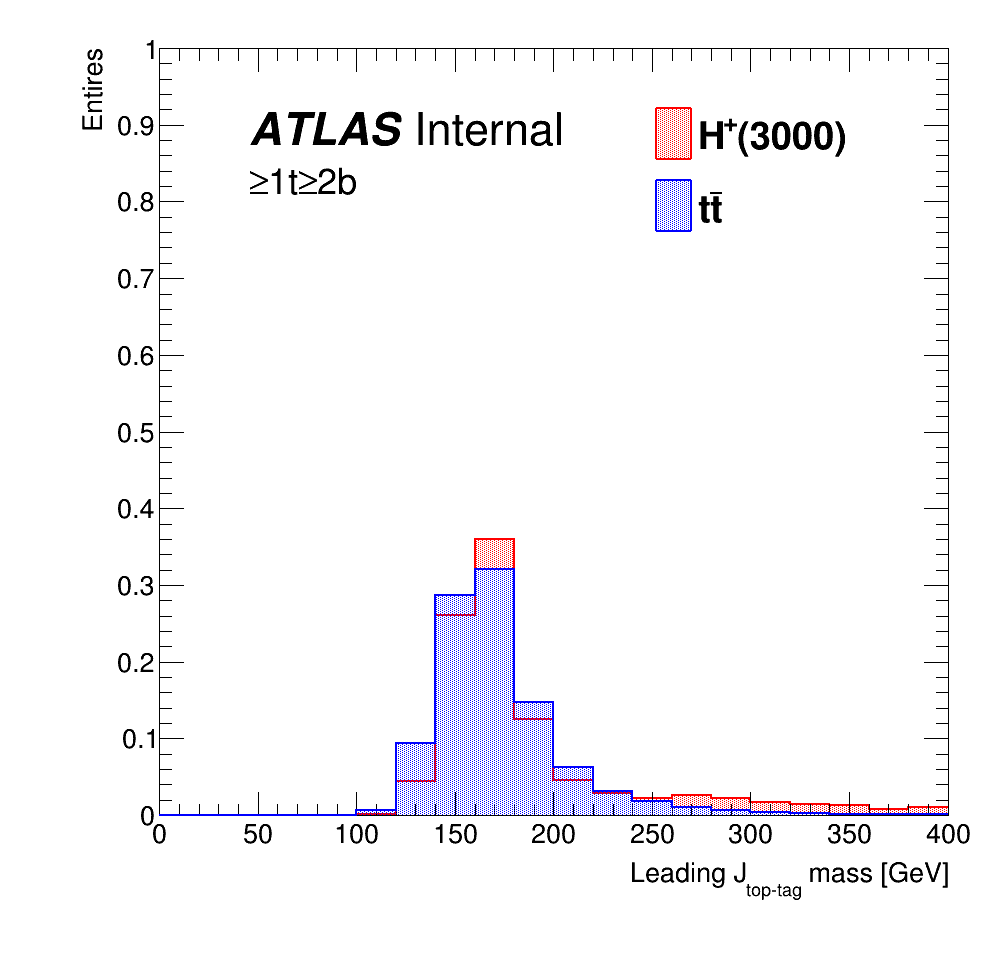
\includegraphics[width=0.25\textwidth]{images/AnalysisStrategy/SOVERB_Hp3000_Contained80_DL1r_70_leadingTop_m_Contained80_DL1r_70.png}
        \label{fig:SOVERB_leadingTop_mass_Hp3000_Contained80_DL1r_70}
      }
      \subfloat[LeadingTop\_pt] {
        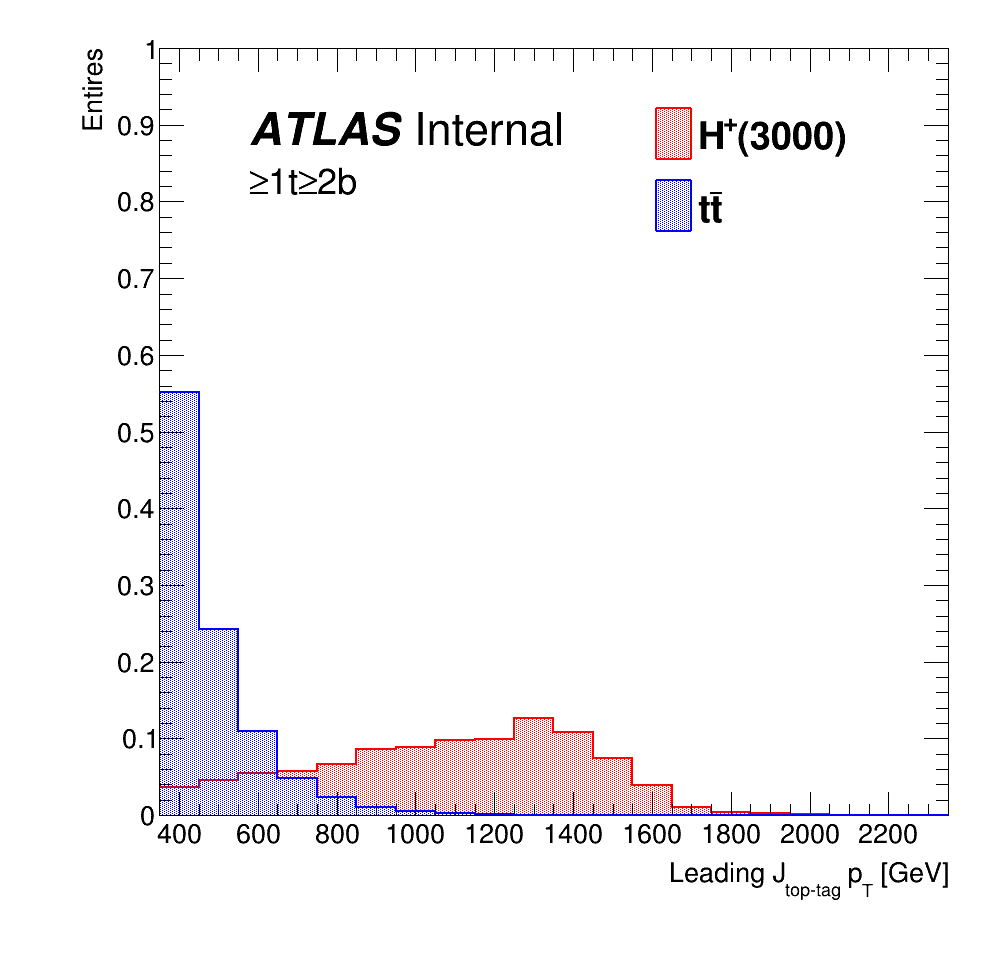
\includegraphics[width=0.25\textwidth]{images/AnalysisStrategy/SOVERB_Hp3000_Contained80_DL1r_70_leadingTop_pt_Contained80_DL1r_70.png}
        \label{fig:SOVERB_leadingTop_pt_Hp3000_Contained80_DL1r_70}
      }
      \subfloat[M\_tb] {
        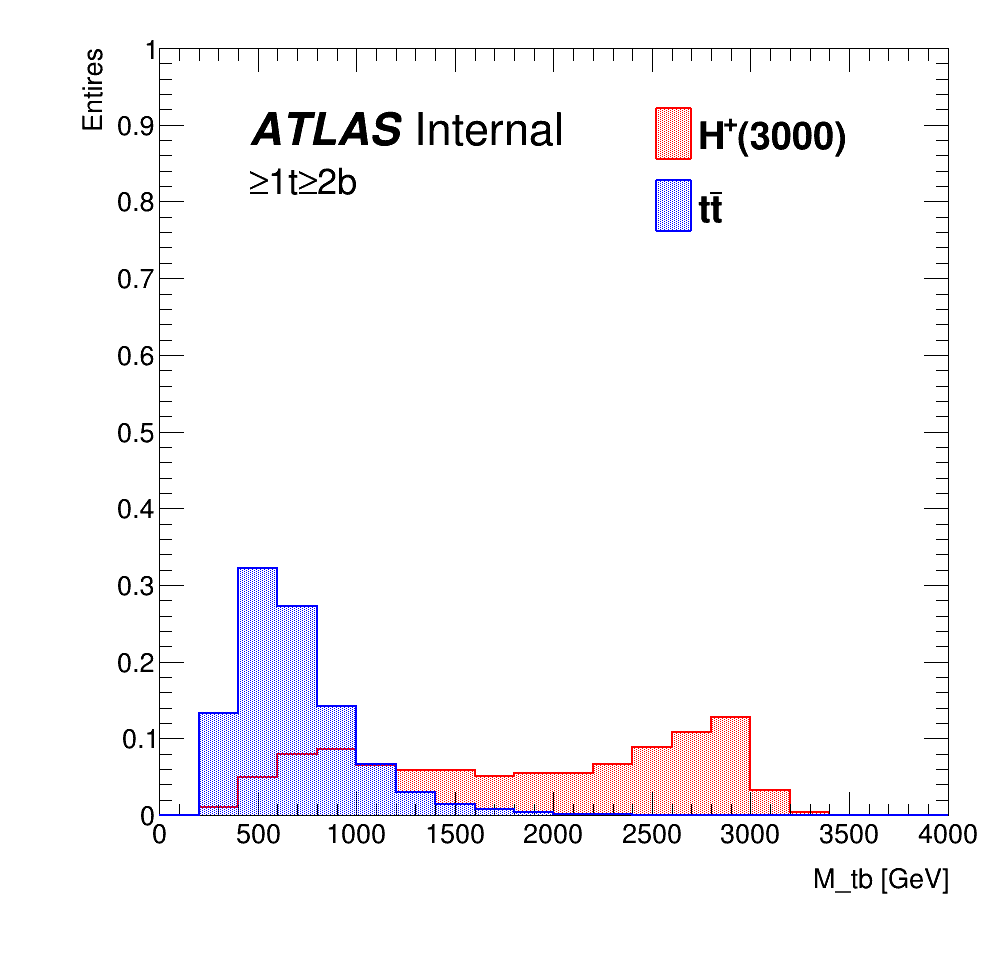
\includegraphics[width=0.25\textwidth]{images/AnalysisStrategy/SOVERB_Hp3000_Contained80_DL1r_70_tb_m_Contained80_DL1r_70.png}
        \label{fig:SOVERB_M_tb_Hp3000_Contained80_DL1r_70}
      }\\
      \subfloat[Pt\_tb] {
        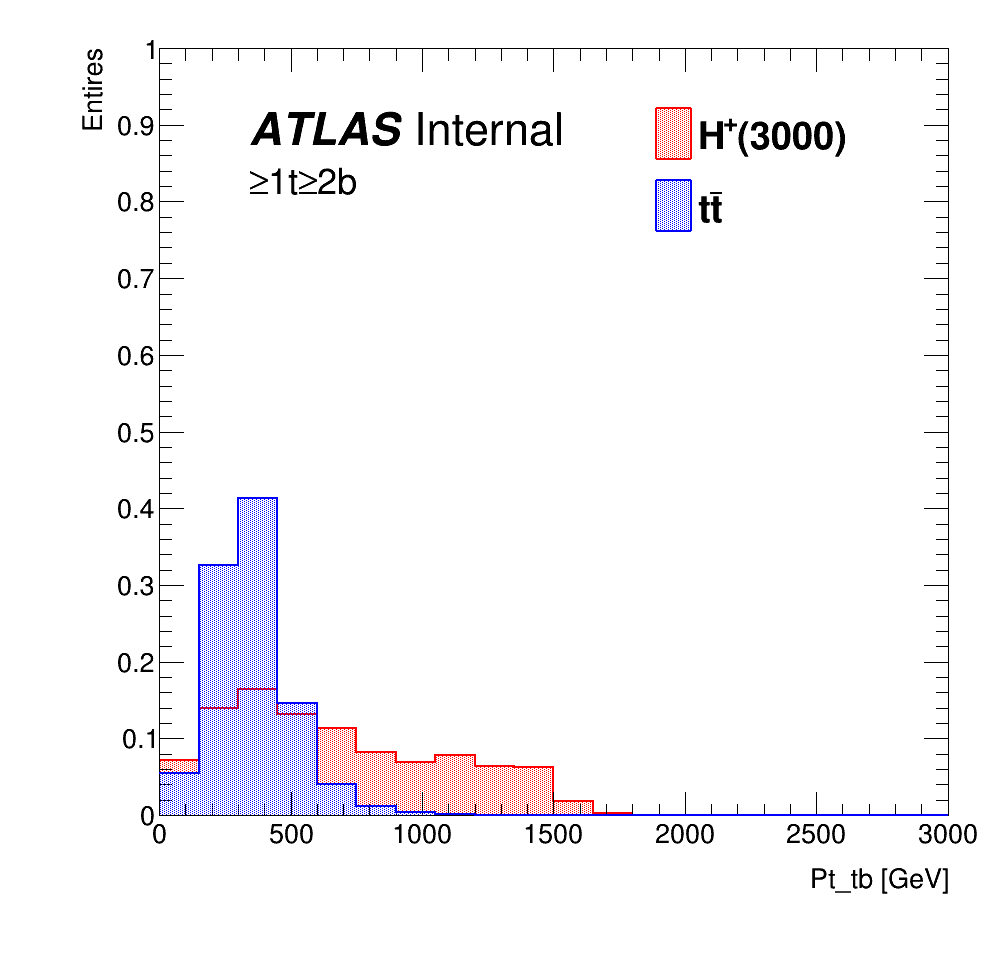
\includegraphics[width=0.25\textwidth]{images/AnalysisStrategy/SOVERB_Hp3000_Contained80_DL1r_70_tb_pt_Contained80_DL1r_70.png}
        \label{fig:SOVERB_Pt_tb_Hp3000_Contained80_DL1r_70}
      }
      \caption{Comparison of input variables for BDT training between $H^{+}$ and $t\bar{t}+\text{jets}$ events under 3000 GeV $H^{+}$ mass hypothesis in the SR.}
      \label{fig:SOVERB_Hp3000_Contained80_DL1r_70}
    \end{figure}

    \item{\textbf{Results of BDT training}}\mbox{}\\
    The BDT output distributions for $H^{+}$ signal and background events in the SR for different values of the $H^+$ mass are shown in Figure \ref{fig:BDTTrainingResults_Hp1000} to \ref{fig:BDTTrainingResults_Hp3000}, together with receiver operating characteristic (ROC) curves.

    %--- BDT template H+(1000)
    \begin{figure}[H]
      \centering
      \subfloat[BDT output]{
        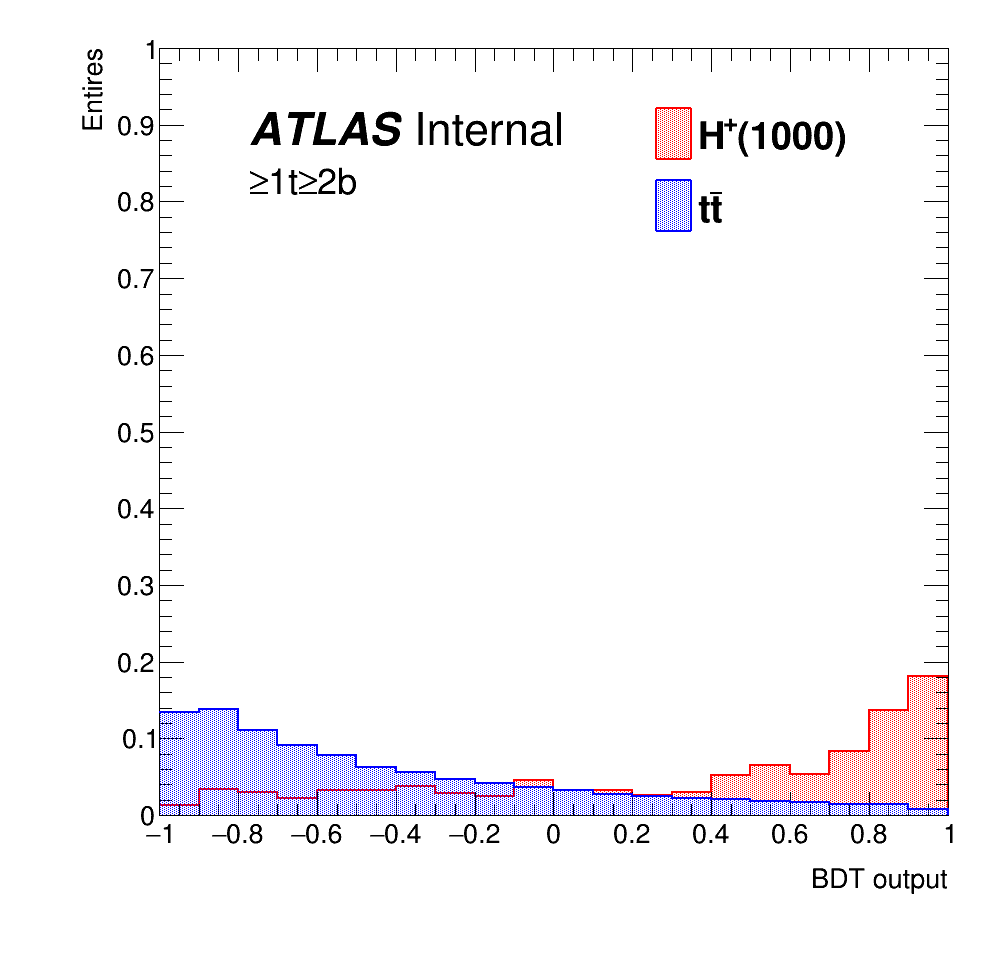
\includegraphics[width=0.45\textwidth]{images/AnalysisStrategy/BDTOutput_Hp1000_Contained80_DL1r_70.png}
        \label{fig:BDTOutput_Hp1000}
      }
      \subfloat[ROC curve]{
        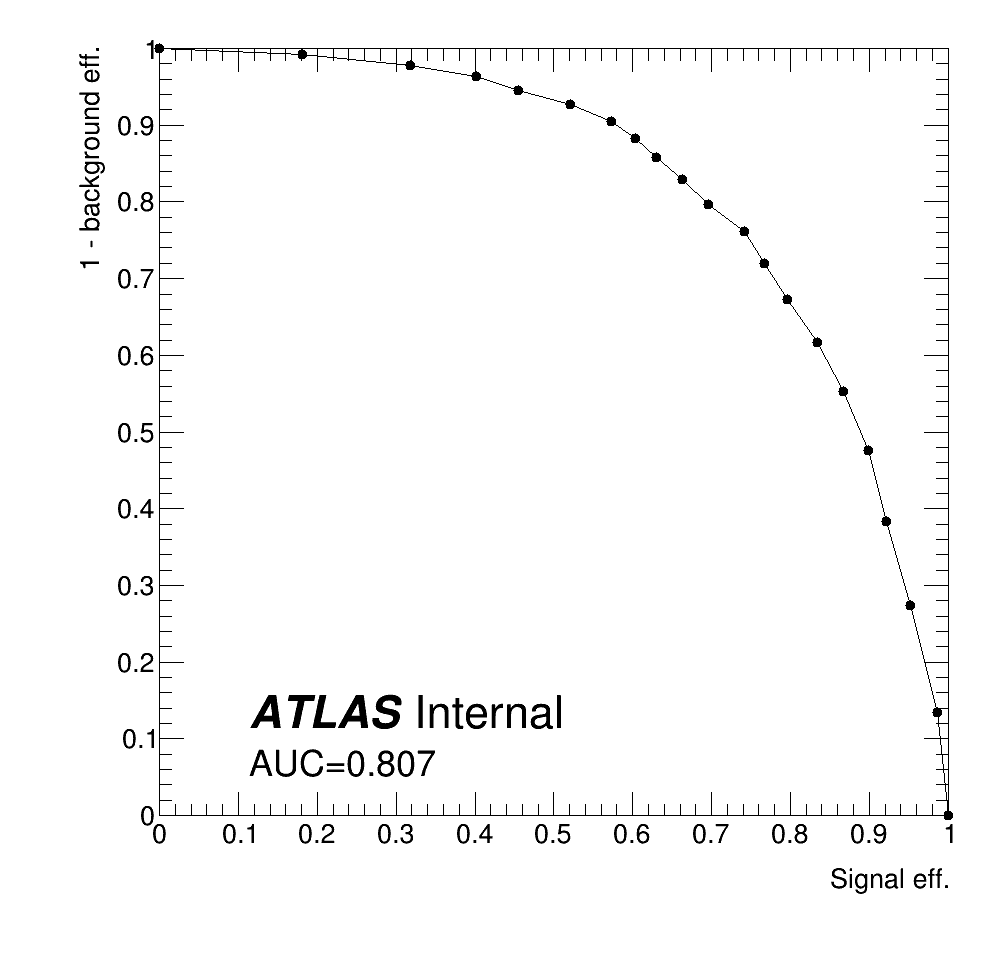
\includegraphics[width=0.45\textwidth]{images/AnalysisStrategy/ROCCurve_Hp1000_Contained80_DL1r_70.png}
        \label{fig:ROCCurve_Hp1000}
      }
      \caption{BDT distribution and ROC curve for the 1000 GeV $H^{+}$ mass hypothesis.}
      \label{fig:BDTTrainingResults_Hp1000}
    \end{figure}
    
    %--- BDT template H+(1200)
    \begin{figure}[H]
      \centering
      \subfloat[BDT output]{
        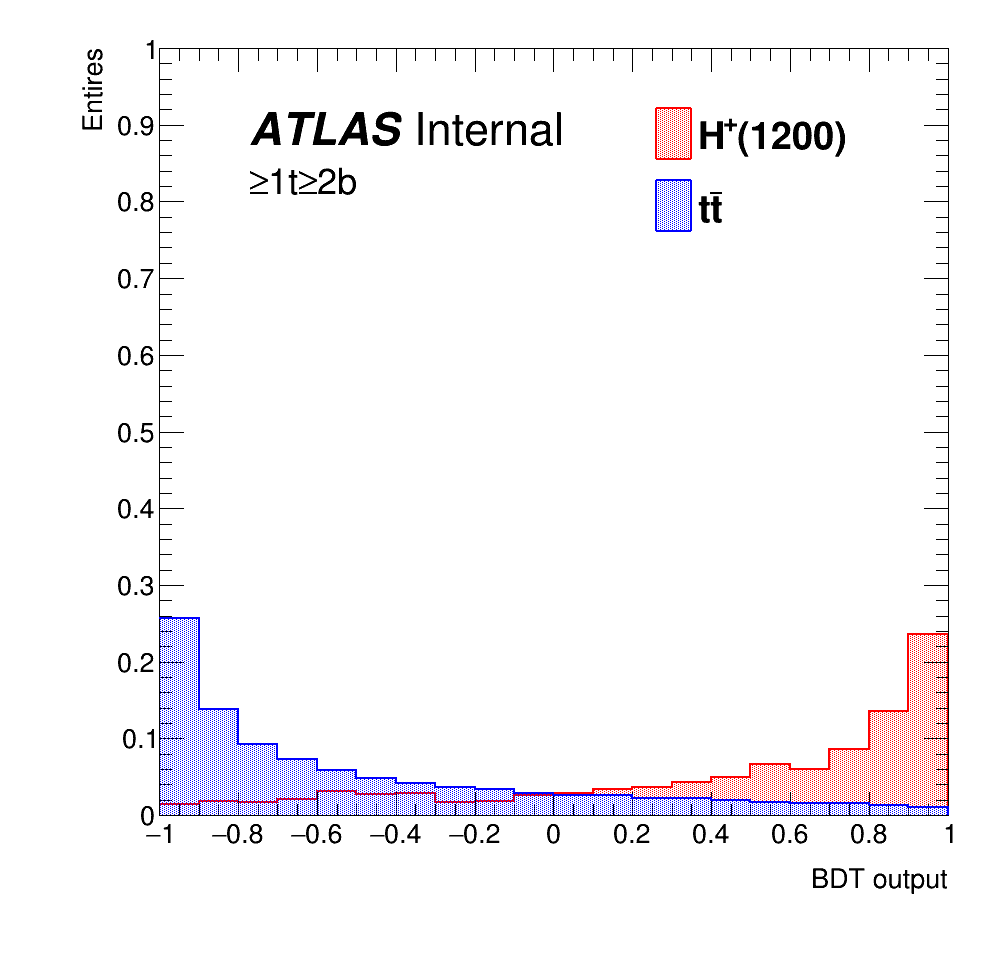
\includegraphics[width=0.45\textwidth]{images/AnalysisStrategy/BDTOutput_Hp1200_Contained80_DL1r_70.png}
        \label{fig:BDTOutput_Hp1200}
      }
      \subfloat[ROC curve]{
        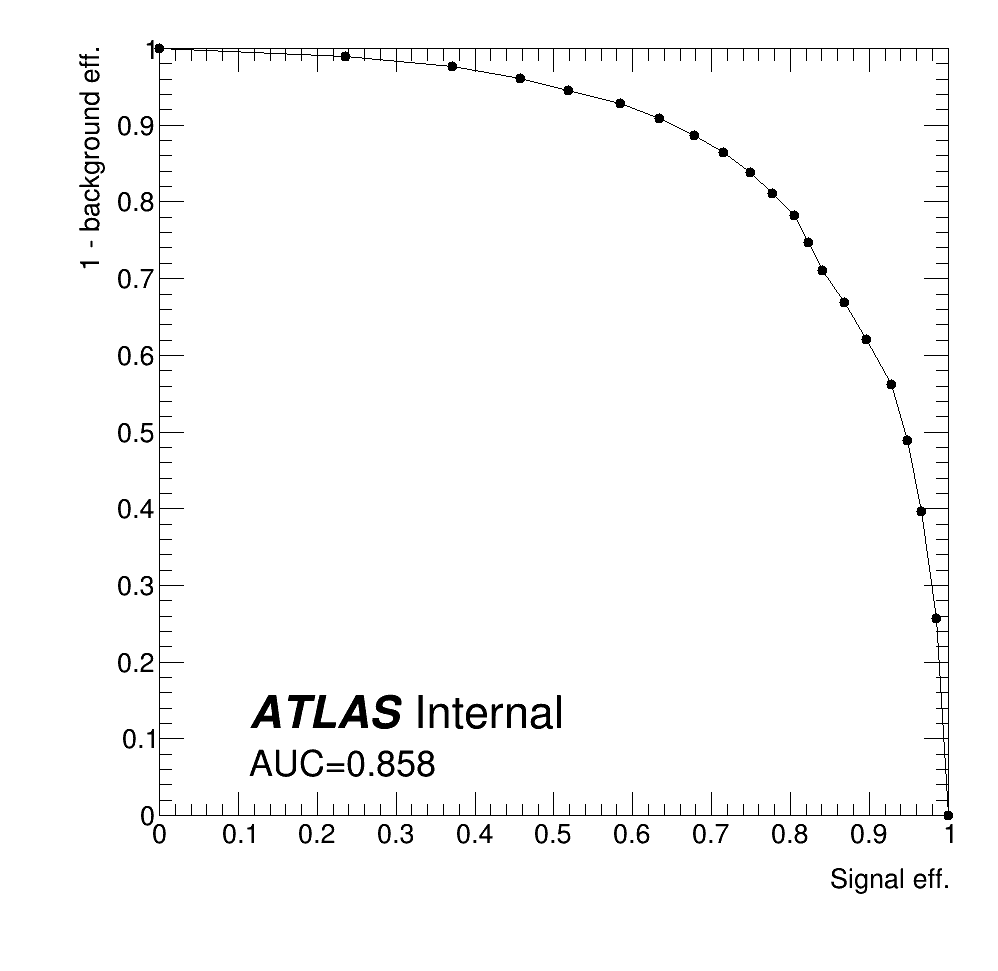
\includegraphics[width=0.45\textwidth]{images/AnalysisStrategy/ROCCurve_Hp1200_Contained80_DL1r_70.png}
        \label{fig:ROCCurve_Hp1200}
      }
      \caption{BDT distribution and ROC curve for the 1200 GeV $H^{+}$ mass hypothesis.}
      \label{fig:BDTTrainingResults_Hp1200}
    \end{figure}
    
    %--- BDT template H+(1400)
    \begin{figure}[H]
      \centering
      \subfloat[BDT output]{
        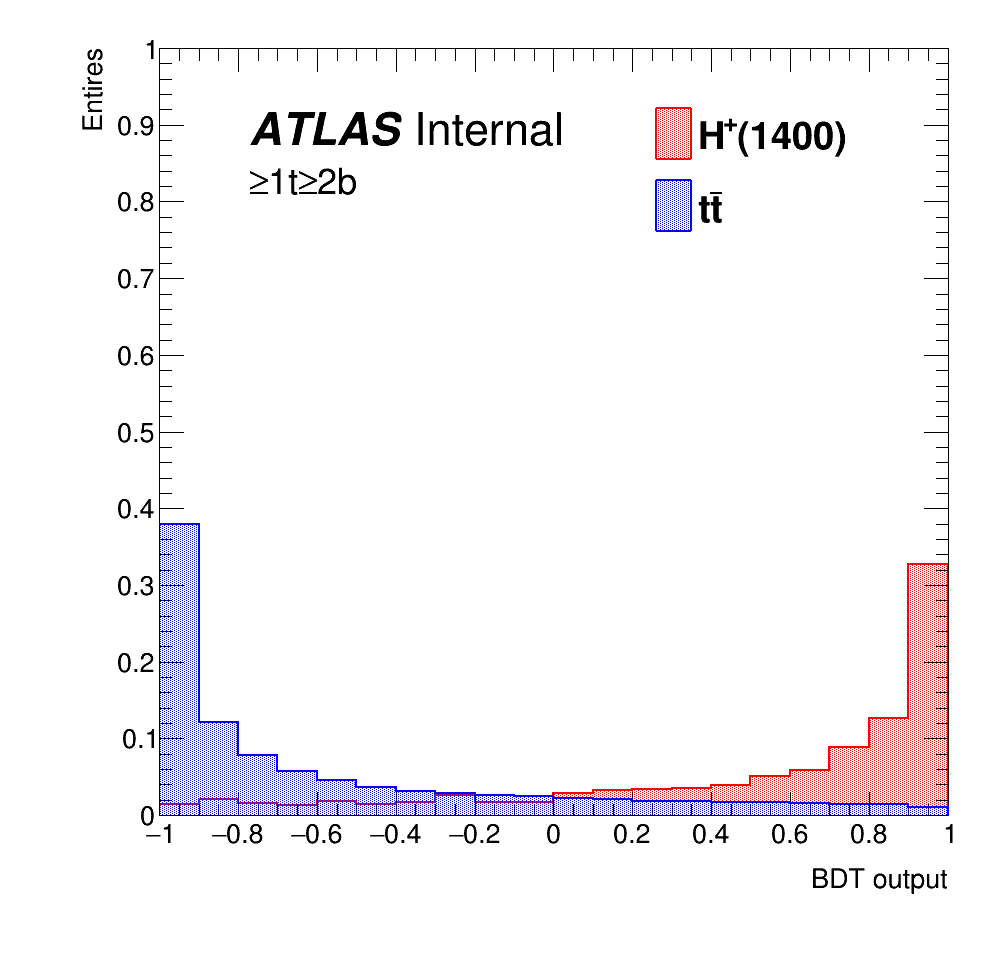
\includegraphics[width=0.45\textwidth]{images/AnalysisStrategy/BDTOutput_Hp1400_Contained80_DL1r_70.png}
        \label{fig:BDTOutput_Hp1400}
      }
      \subfloat[ROC curve]{
        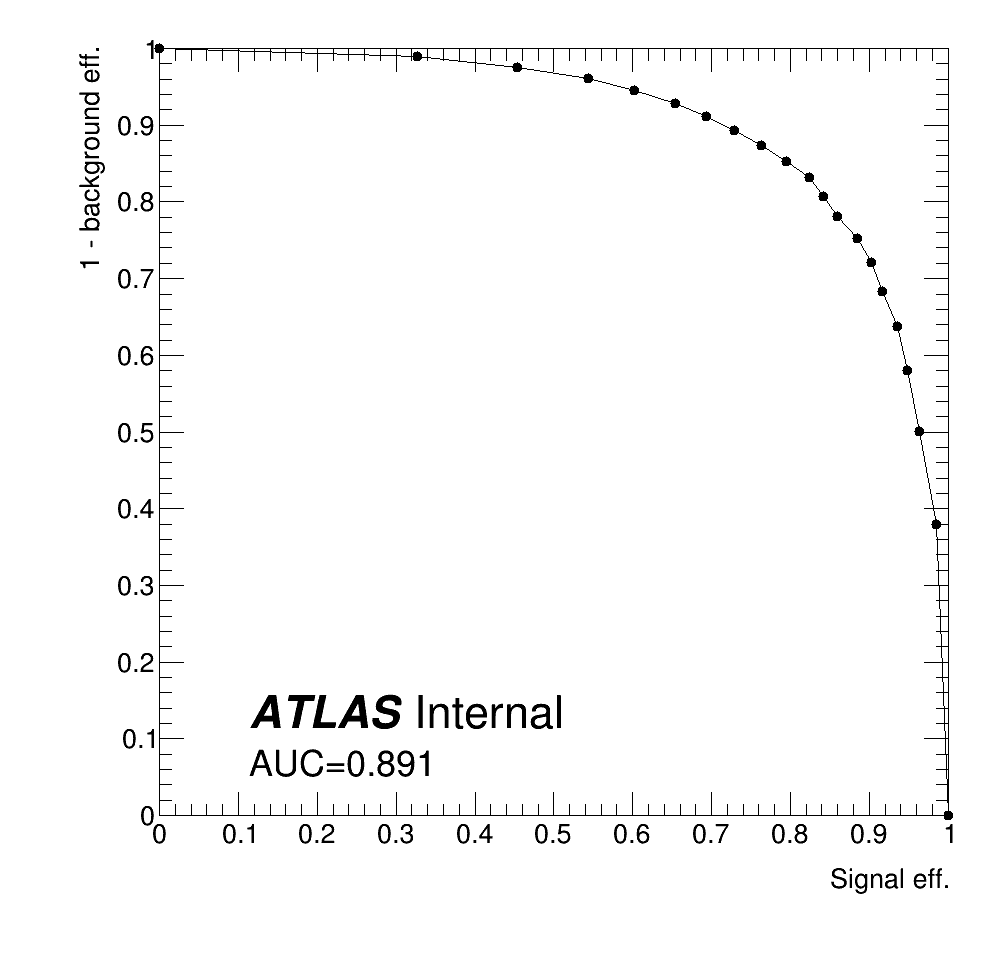
\includegraphics[width=0.45\textwidth]{images/AnalysisStrategy/ROCCurve_Hp1400_Contained80_DL1r_70.png}
        \label{fig:ROCCurve_Hp1400}
      }
      \caption{BDT distribution and ROC curve for the 1400 GeV $H^{+}$ mass hypothesis.}
      \label{fig:BDTTrainingResults_Hp1400}
    \end{figure}
    
    %--- BDT template H+(1600)
    \begin{figure}[H]
      \centering
      \subfloat[BDT output]{
        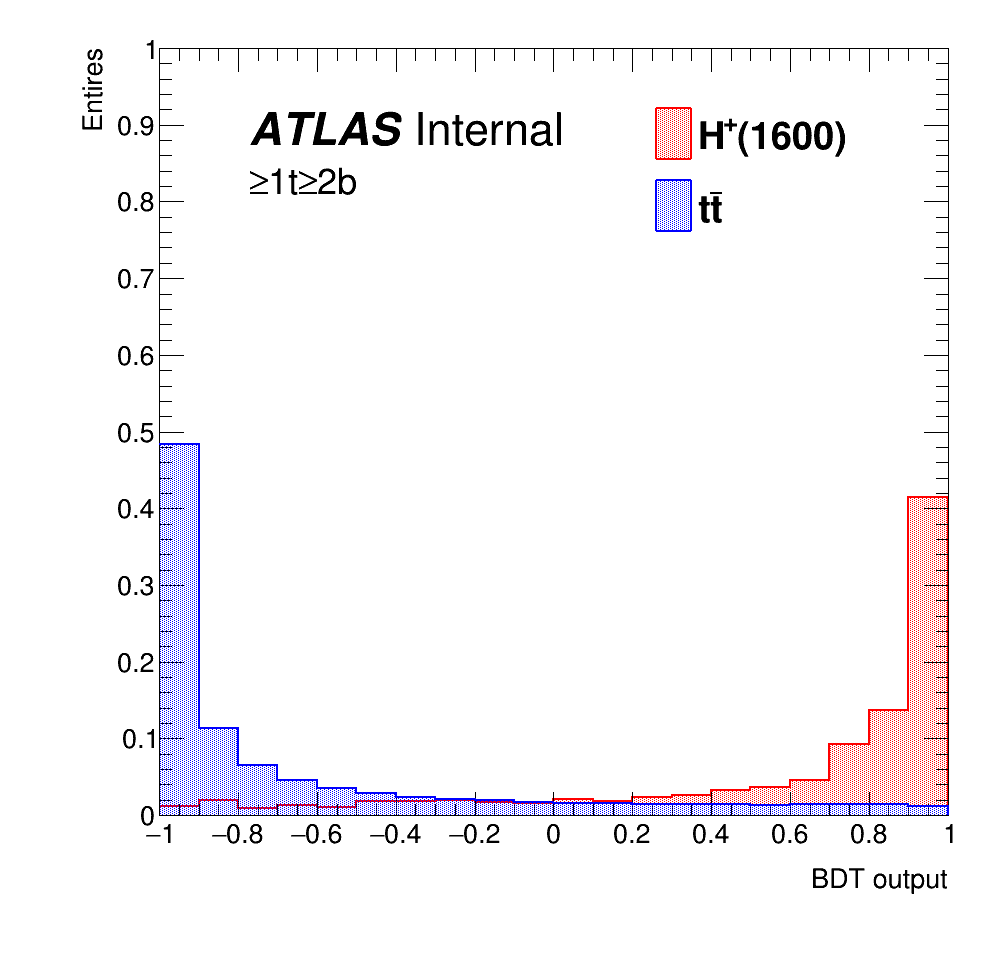
\includegraphics[width=0.45\textwidth]{images/AnalysisStrategy/BDTOutput_Hp1600_Contained80_DL1r_70.png}
        \label{fig:BDTOutput_Hp1600}
      }
      \subfloat[ROC curve]{
        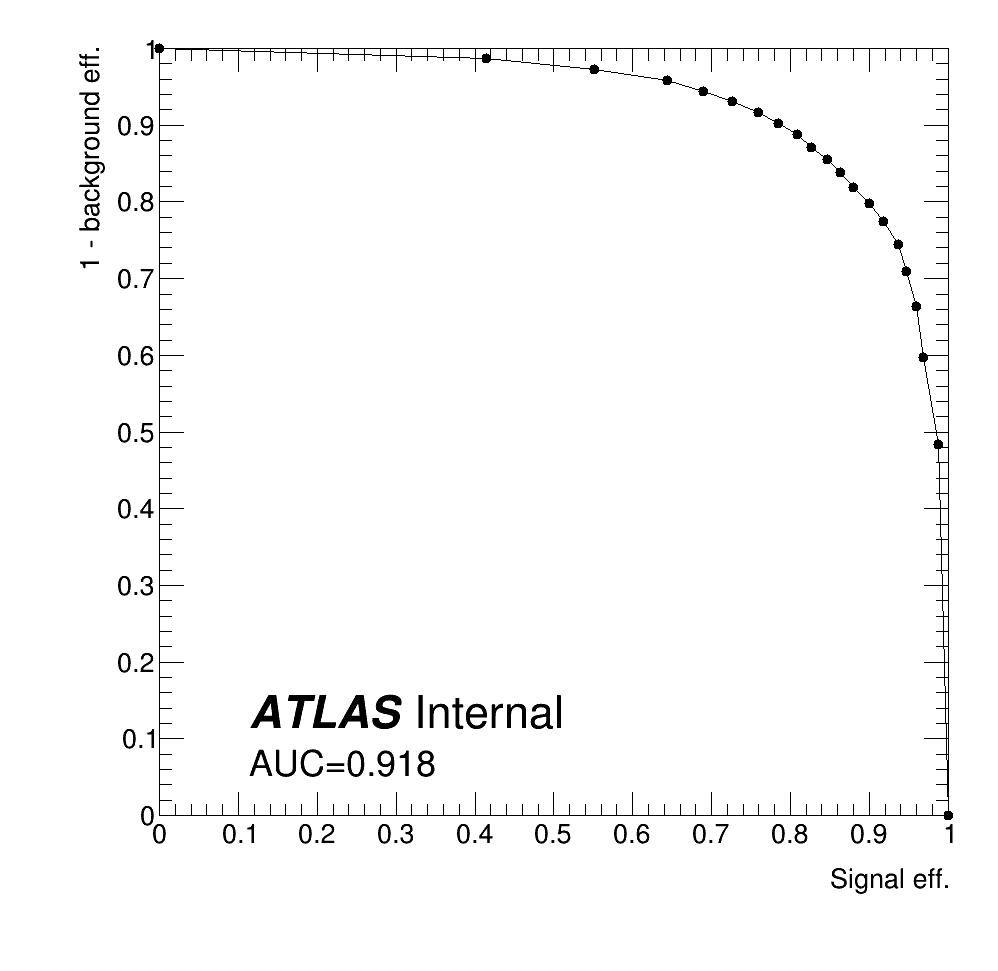
\includegraphics[width=0.45\textwidth]{images/AnalysisStrategy/ROCCurve_Hp1600_Contained80_DL1r_70.png}
        \label{fig:ROCCurve_Hp1600}
      }
      \caption{BDT distribution and ROC curve for the 1600 GeV $H^{+}$ mass hypothesis.}
      \label{fig:BDTTrainingResults_Hp1600}
    \end{figure}
    
    %--- BDT template H+(1800)
    \begin{figure}[H]
      \centering
      \subfloat[BDT output]{
        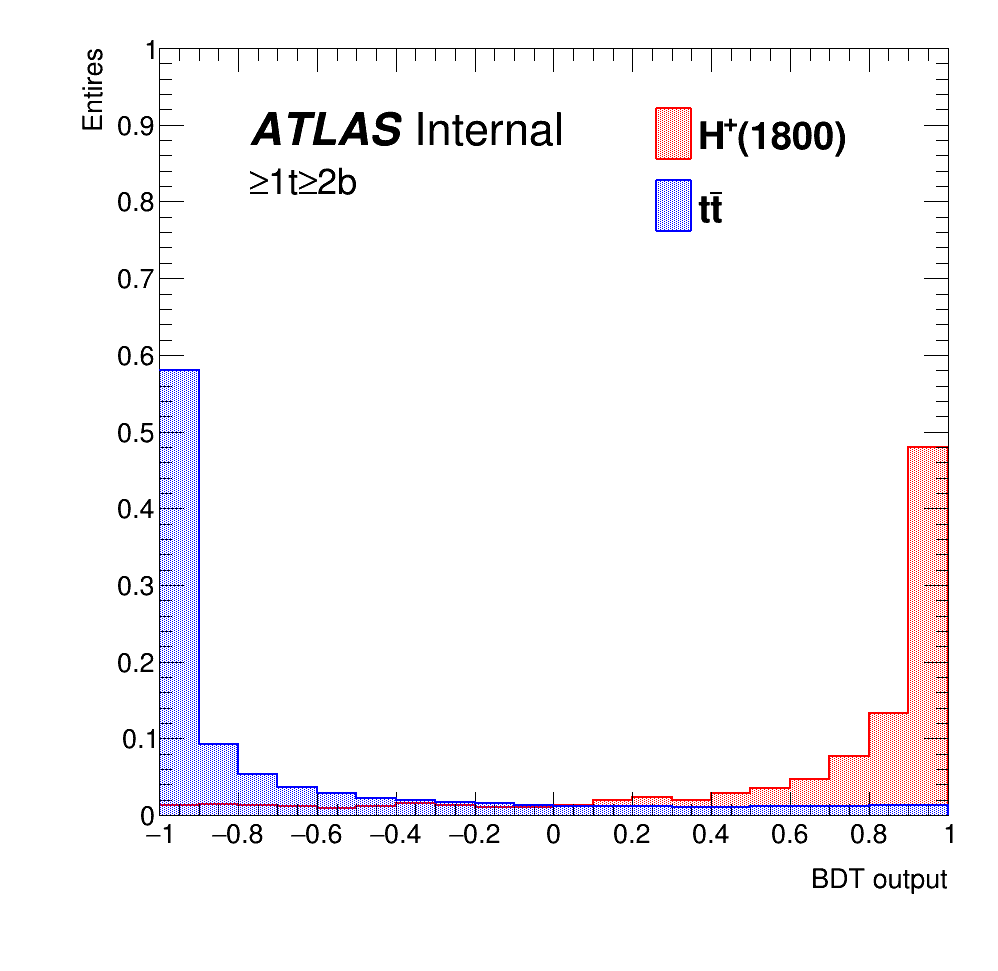
\includegraphics[width=0.45\textwidth]{images/AnalysisStrategy/BDTOutput_Hp1800_Contained80_DL1r_70.png}
        \label{fig:BDTOutput_Hp1800}
      }
      \subfloat[ROC curve]{
        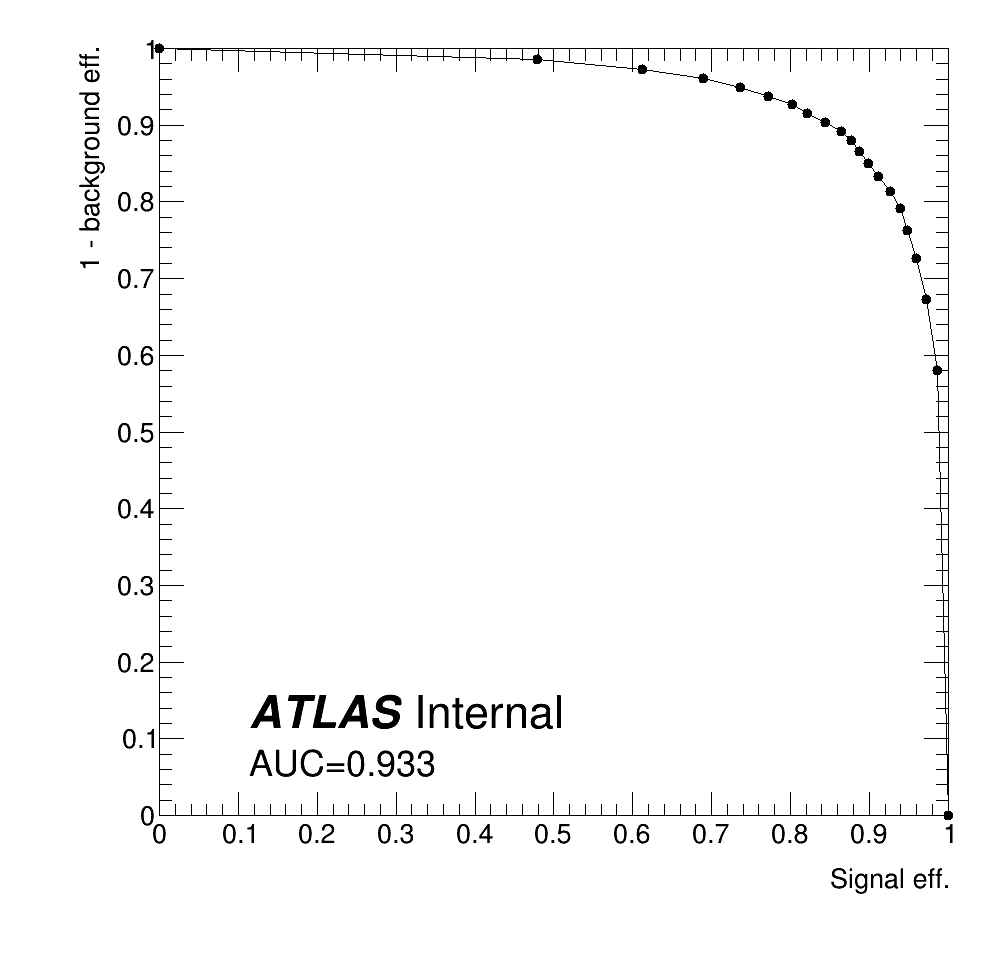
\includegraphics[width=0.45\textwidth]{images/AnalysisStrategy/ROCCurve_Hp1800_Contained80_DL1r_70.png}
        \label{fig:ROCCurve_Hp1800}
      }
      \caption{BDT distribution and ROC curve for the 1800 GeV $H^{+}$ mass hypothesis.}
      \label{fig:BDTTrainingResults_Hp1800}
    \end{figure}
    
    %--- BDT template H+(2000)
    \begin{figure}[H]
      \centering
      \subfloat[BDT output]{
        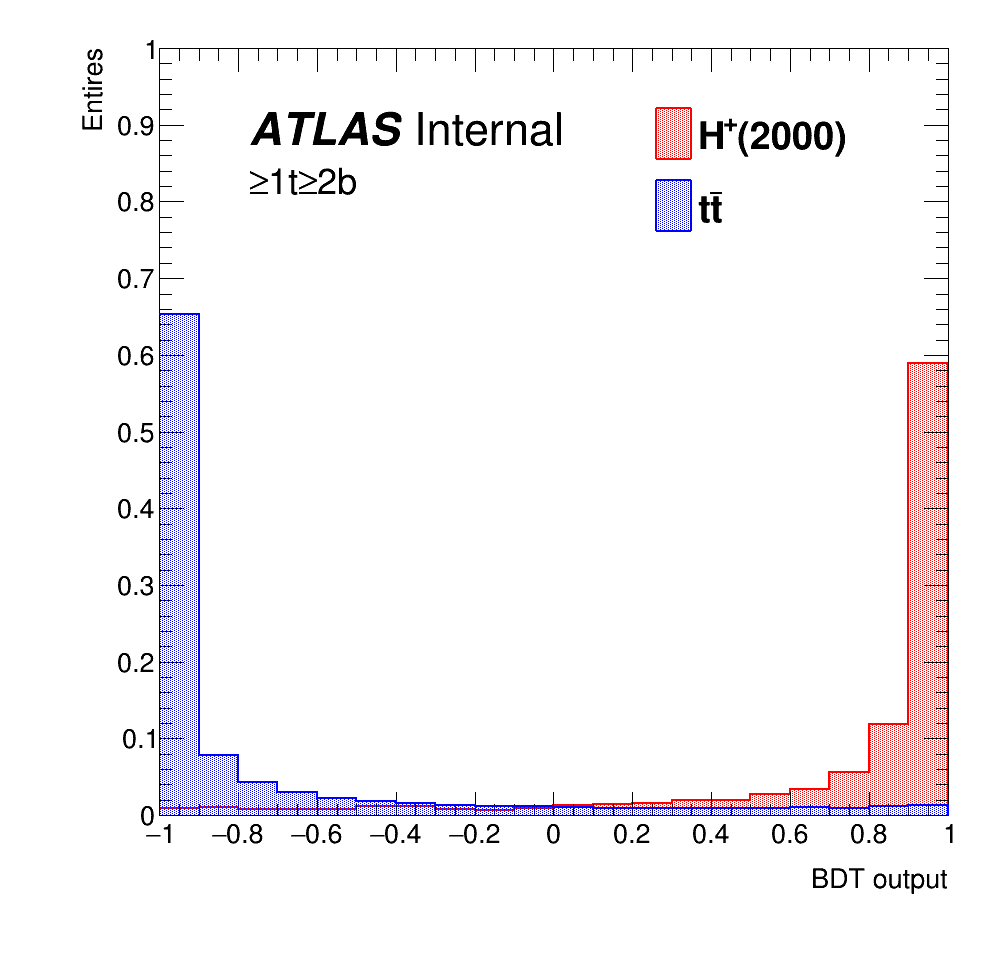
\includegraphics[width=0.45\textwidth]{images/AnalysisStrategy/BDTOutput_Hp2000_Contained80_DL1r_70.png}
        \label{fig:BDTOutput_Hp2000}
      }
      \subfloat[ROC curve]{
        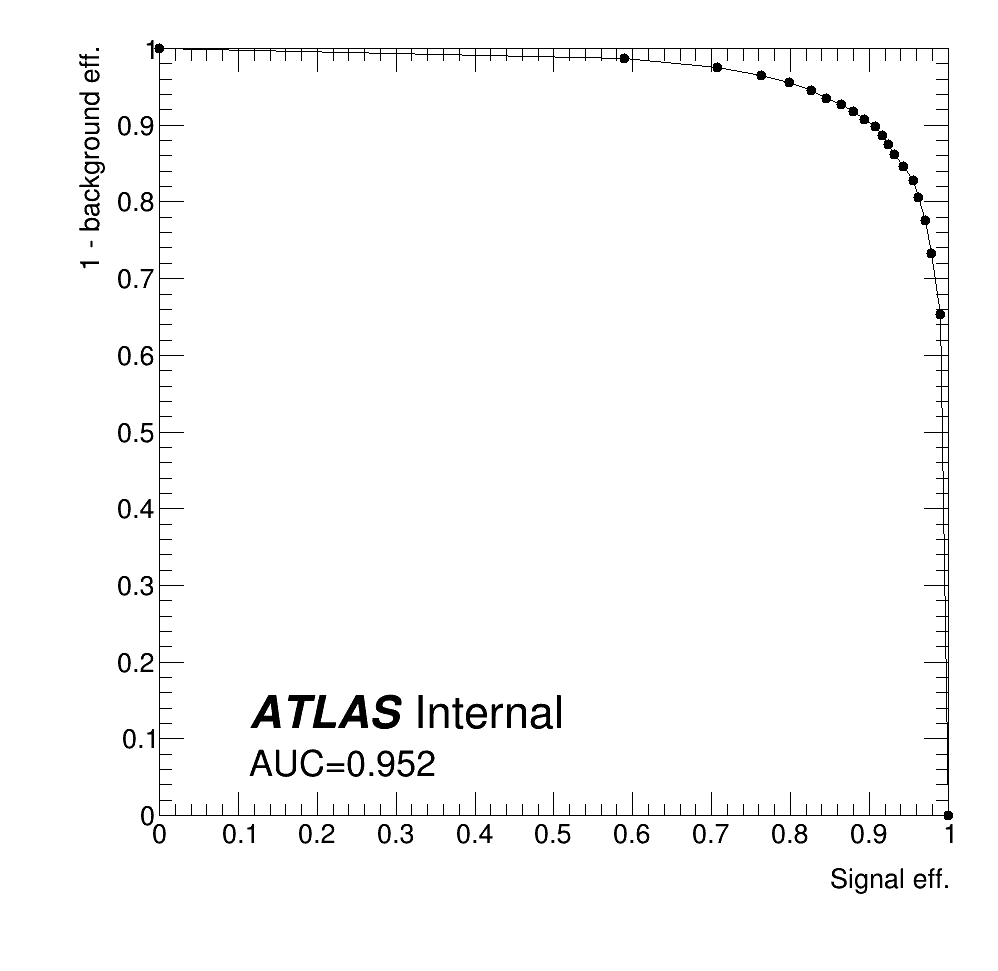
\includegraphics[width=0.45\textwidth]{images/AnalysisStrategy/ROCCurve_Hp2000_Contained80_DL1r_70.png}
        \label{fig:ROCCurve_Hp2000}
      }
      \caption{BDT distribution and ROC curve for the 2000 GeV $H^{+}$ mass hypothesis.}
      \label{fig:BDTTrainingResults_Hp2000}
    \end{figure}
    
    %--- BDT template H+(2500)
    \begin{figure}[H]
      \centering
      \subfloat[BDT output]{
        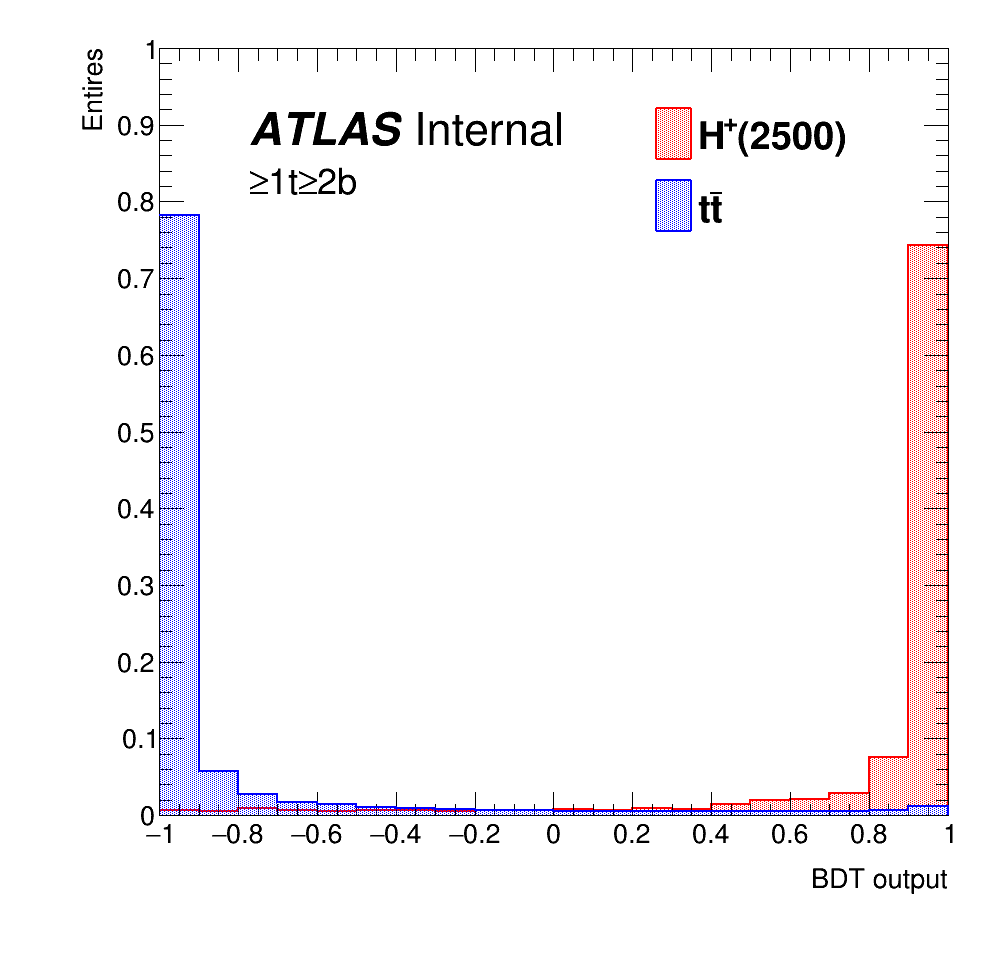
\includegraphics[width=0.45\textwidth]{images/AnalysisStrategy/BDTOutput_Hp2500_Contained80_DL1r_70.png}
        \label{fig:BDTOutput_Hp2500}
      }
      \subfloat[ROC curve]{
        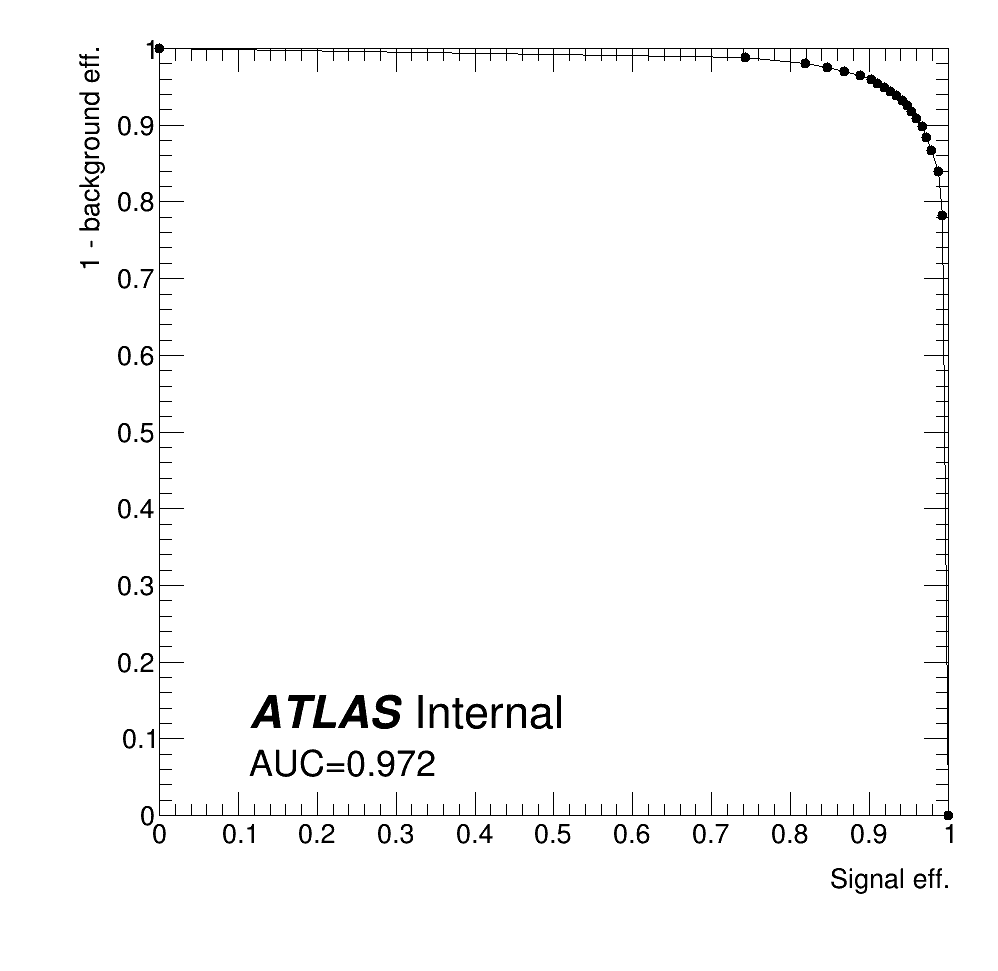
\includegraphics[width=0.45\textwidth]{images/AnalysisStrategy/ROCCurve_Hp2500_Contained80_DL1r_70.png}
        \label{fig:ROCCurve_Hp2500}
      }
      \caption{BDT distribution and ROC curve for the 2500 GeV $H^{+}$ mass hypothesis.}
      \label{fig:BDTTrainingResults_Hp2500}
    \end{figure}
    
    %--- BDT template H+(3000)
    \begin{figure}[H]
      \centering
      \subfloat[BDT output]{
        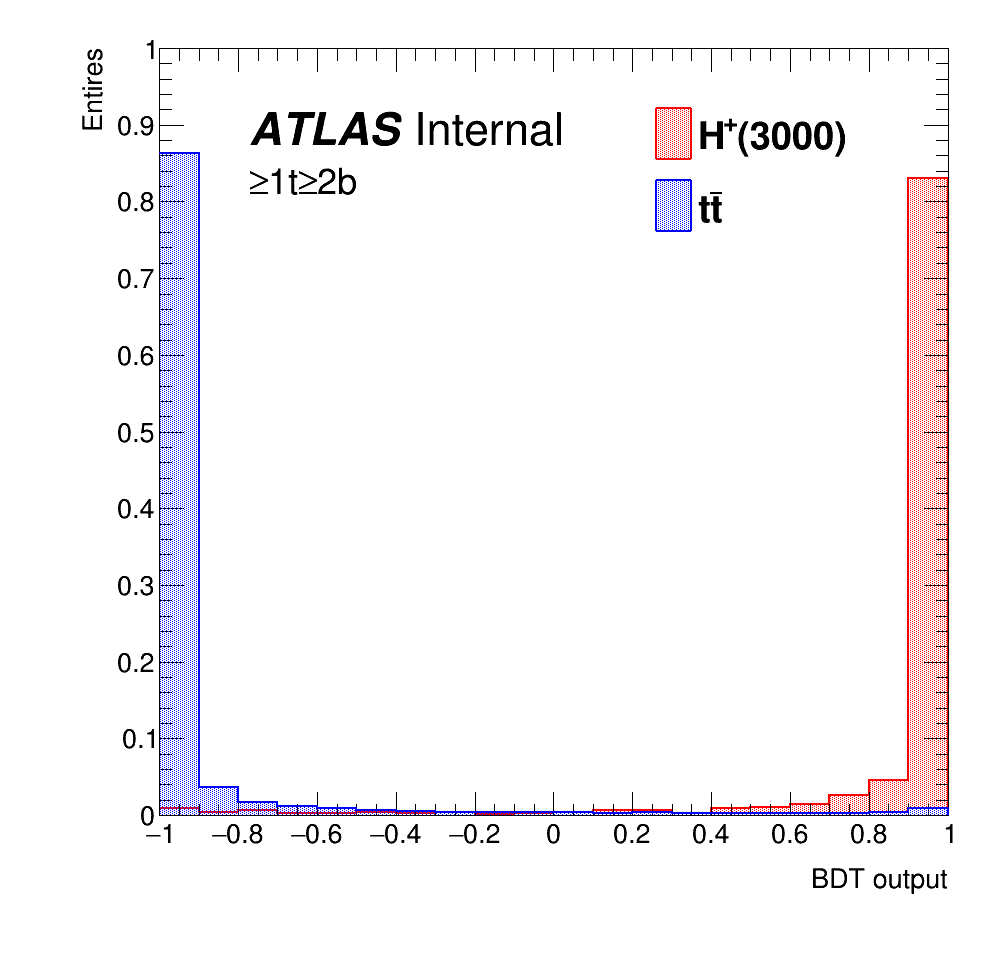
\includegraphics[width=0.45\textwidth]{images/AnalysisStrategy/BDTOutput_Hp3000_Contained80_DL1r_70.png}
        \label{fig:BDTOutput_Hp3000}
      }
      \subfloat[ROC curve]{
        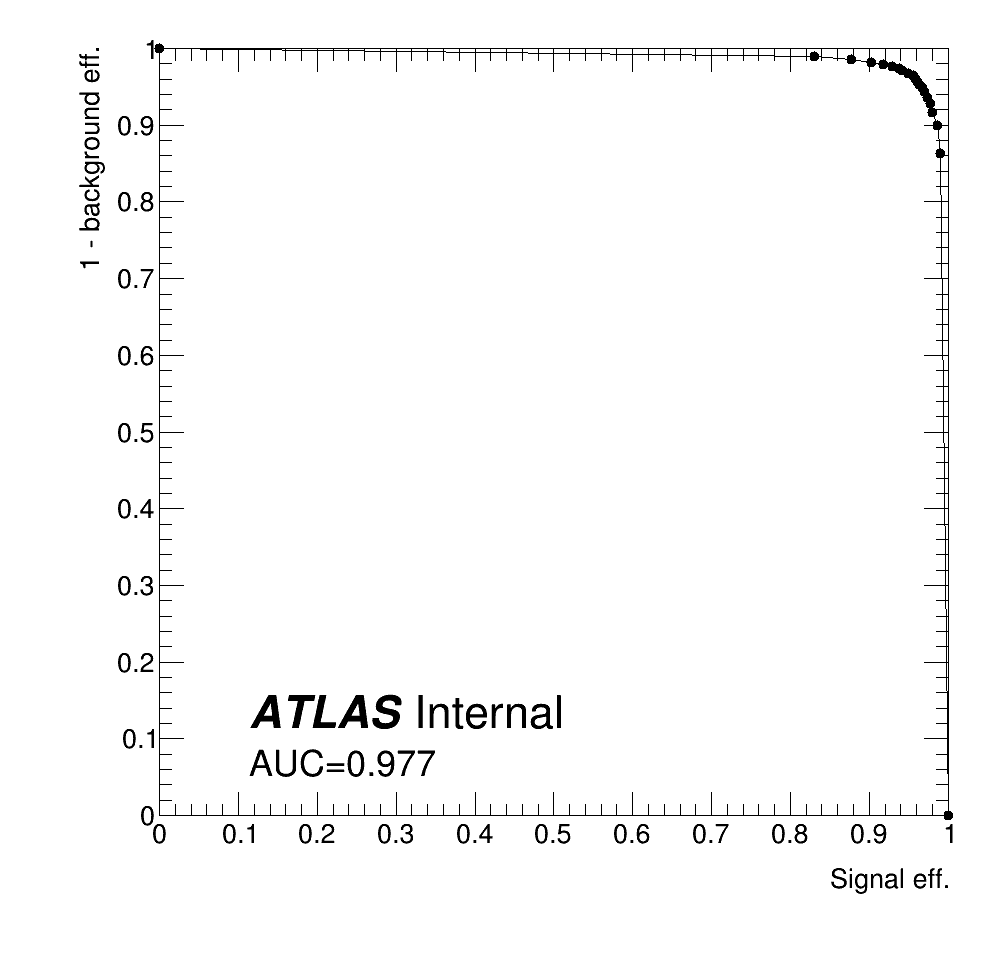
\includegraphics[width=0.45\textwidth]{images/AnalysisStrategy/ROCCurve_Hp3000_Contained80_DL1r_70.png}
        \label{fig:ROCCurve_Hp3000}
      }
      \caption{BDT distribution and ROC curve for the 3000 GeV $H^{+}$ mass hypothesis.}
      \label{fig:BDTTrainingResults_Hp3000}
    \end{figure}

    \item{\textbf{Comparison of BDT distributions between $H^{+} \rightarrow tb$ and  $W' \rightarrow tb$ events}}\mbox{}\\
    BDT distributions for $W' \rightarrow tb$ events are compared with the ones for $H^{+} \rightarrow tb$ events in Figure \ref{fig:CompHpAndWp}. The large differences above their statistic uncertainty are not observed. Therefore, it is expected to be able to obtain comparable sensitivity with $H^{+} \rightarrow tb$ analysis without further optimization using $W' \rightarrow tb$ samples.

    %--- Comparison of BDT outputs between H+ and W'
    \begin{figure}[H]
        \centering
        \subfloat[$M=1.0$ TeV]{
            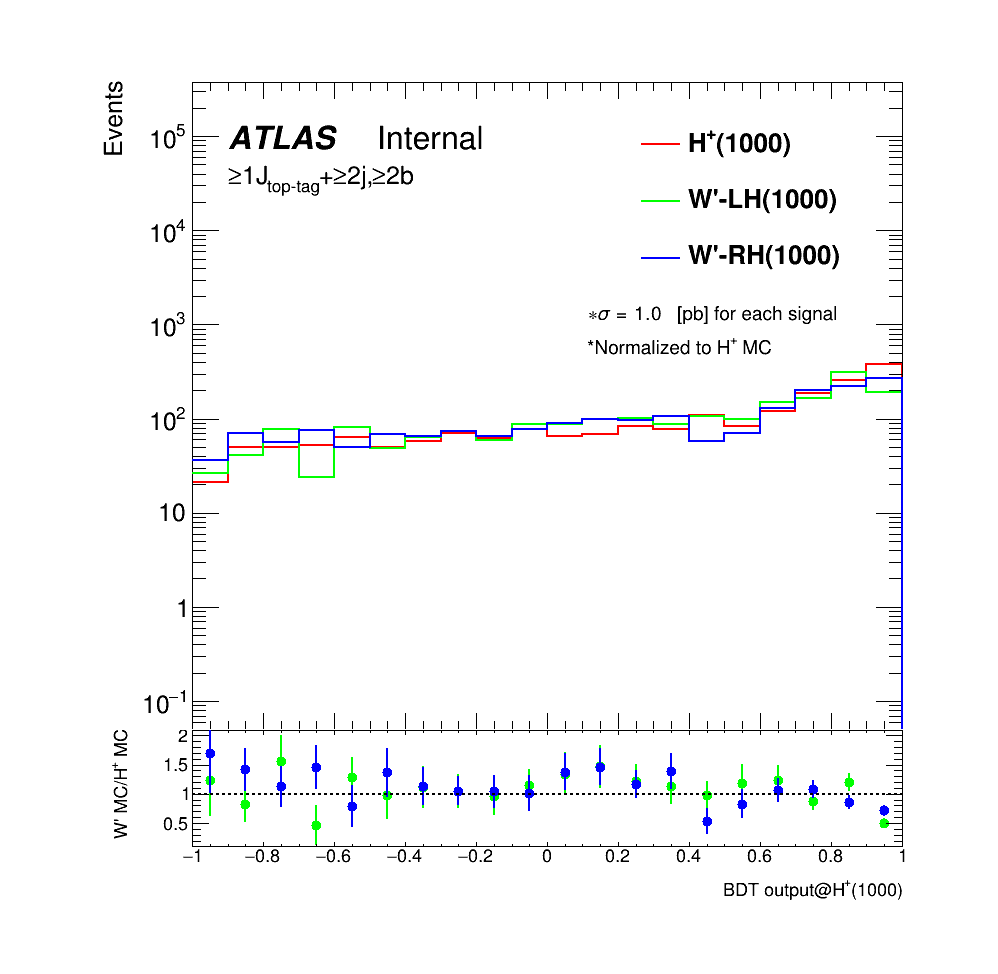
\includegraphics[width=0.45\textwidth]{images/AnalysisStrategy/bdt_Hp1000_1000_geq1tgeq2jgeq2b.png}
            \label{fig:CompHpAndWp_M1000}
        }
        \subfloat[$M=1.2$ TeV]{
            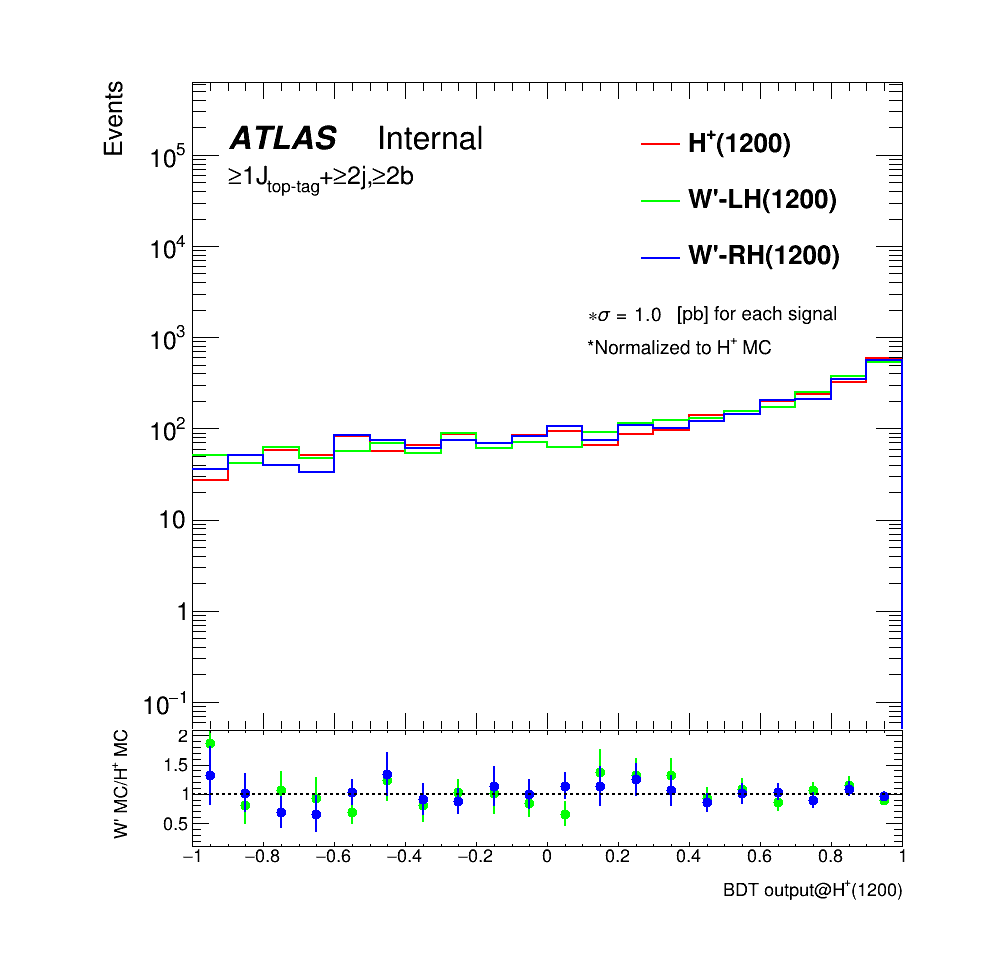
\includegraphics[width=0.45\textwidth]{images/AnalysisStrategy/bdt_Hp1200_1200_geq1tgeq2jgeq2b.png}
            \label{fig:CompHpAndWp_M1200}
        }\\
        \subfloat[$M=1.4$ TeV]{
            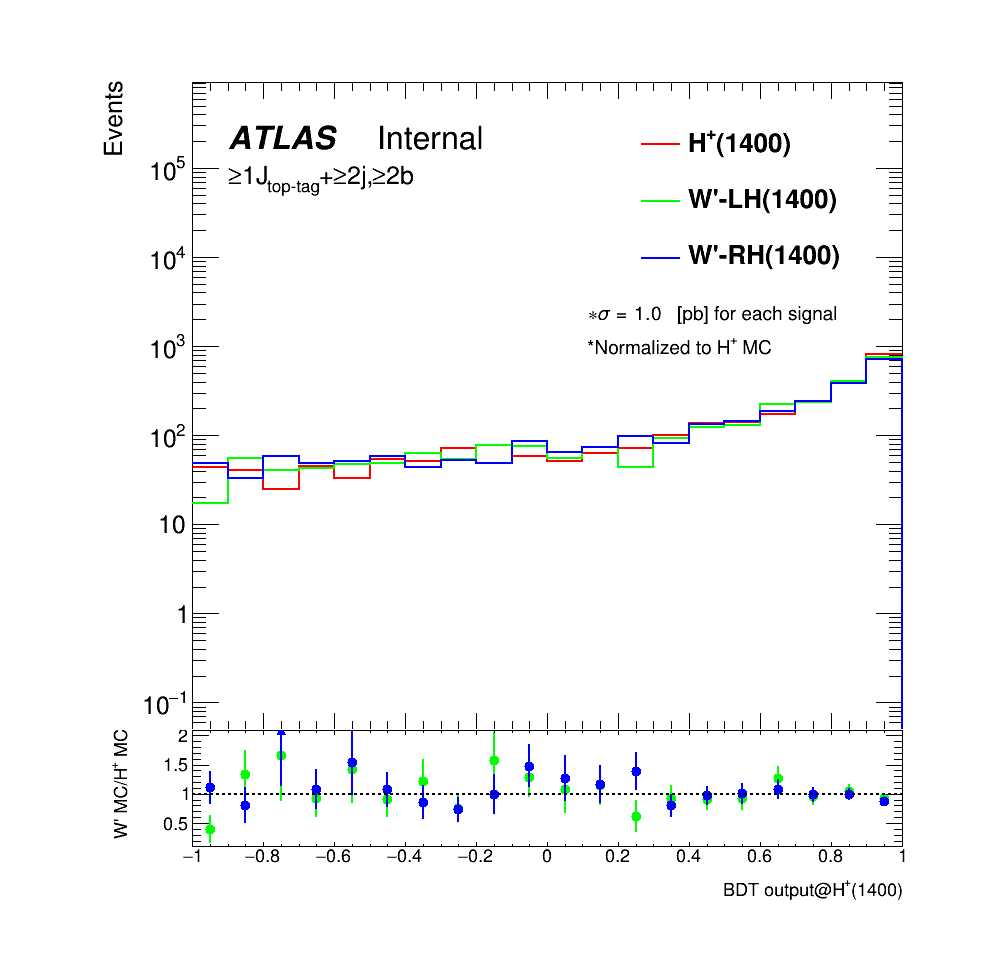
\includegraphics[width=0.45\textwidth]{images/AnalysisStrategy/bdt_Hp1400_1400_geq1tgeq2jgeq2b.png}
            \label{fig:CompHpAndWp_M1400}
        }  
        \subfloat[$M=1.6$ TeV]{
            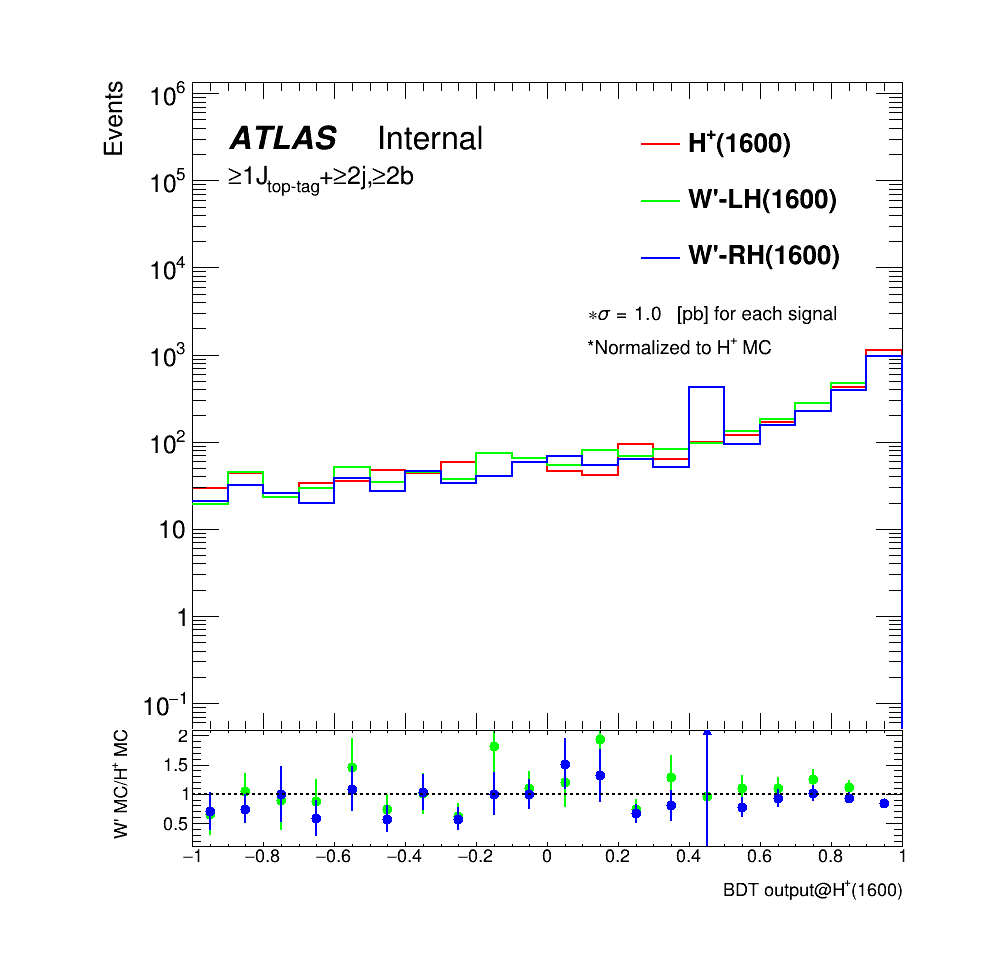
\includegraphics[width=0.45\textwidth]{images/AnalysisStrategy/bdt_Hp1600_1600_geq1tgeq2jgeq2b.png}
            \label{fig:CompHpAndWp_M1600}
        }\\
    \end{figure}
    \begin{figure}[H]
        %\addtocounter{figure}{-1}
        \subfloat[$M=1.8$ TeV]{
             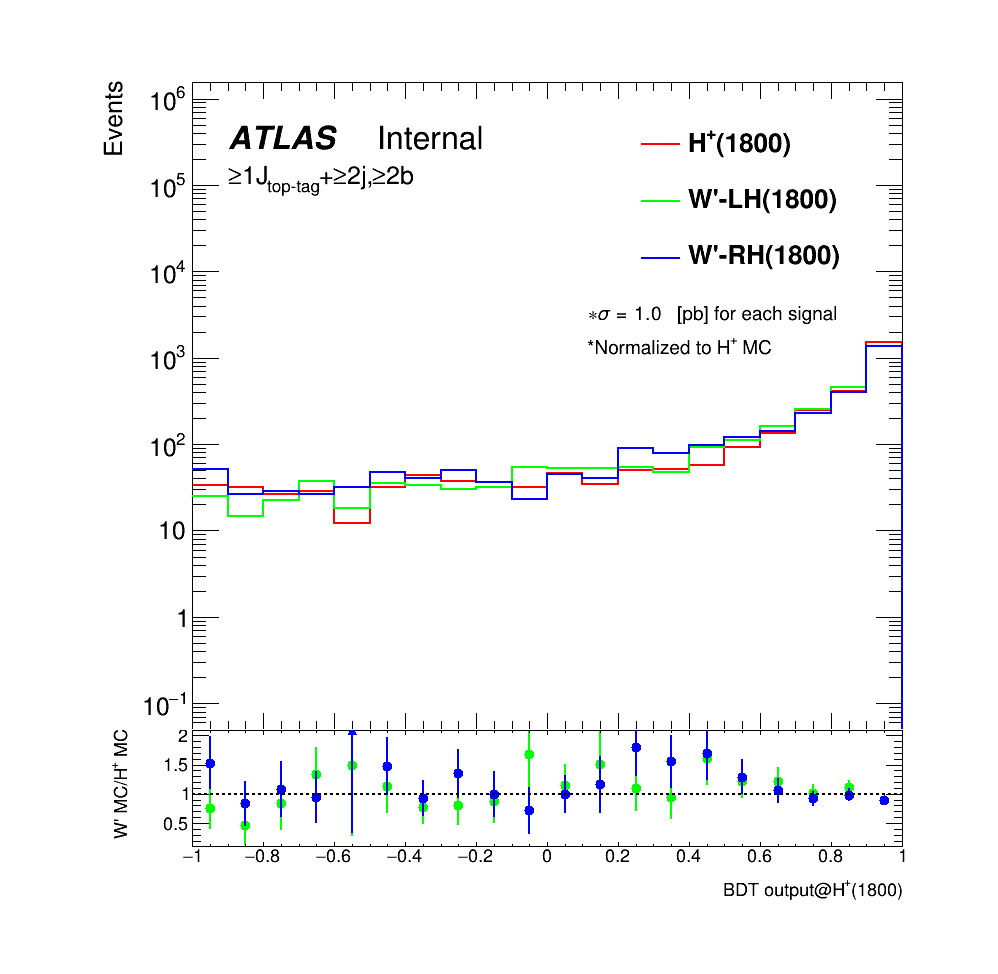
\includegraphics[width=0.45\textwidth]{images/AnalysisStrategy/bdt_Hp1800_1800_geq1tgeq2jgeq2b.png}
             \label{fig:CompHpAndWp_M1800}
        }
        \subfloat[$M=2.0$ TeV]{
            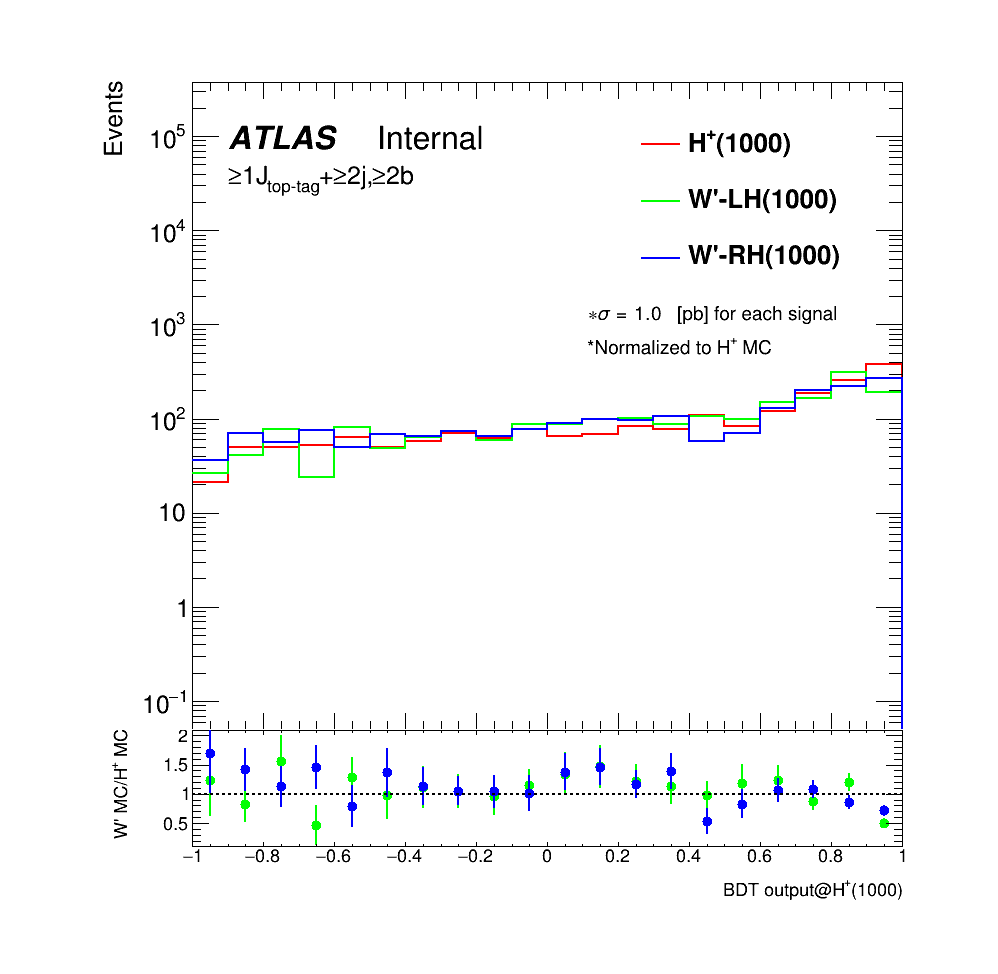
\includegraphics[width=0.45\textwidth]{images/AnalysisStrategy/bdt_Hp1000_1000_geq1tgeq2jgeq2b.png}
            \label{fig:CompHpAndWp_M2000}
        }\\
        \subfloat[$M=2.5$ TeV]{
            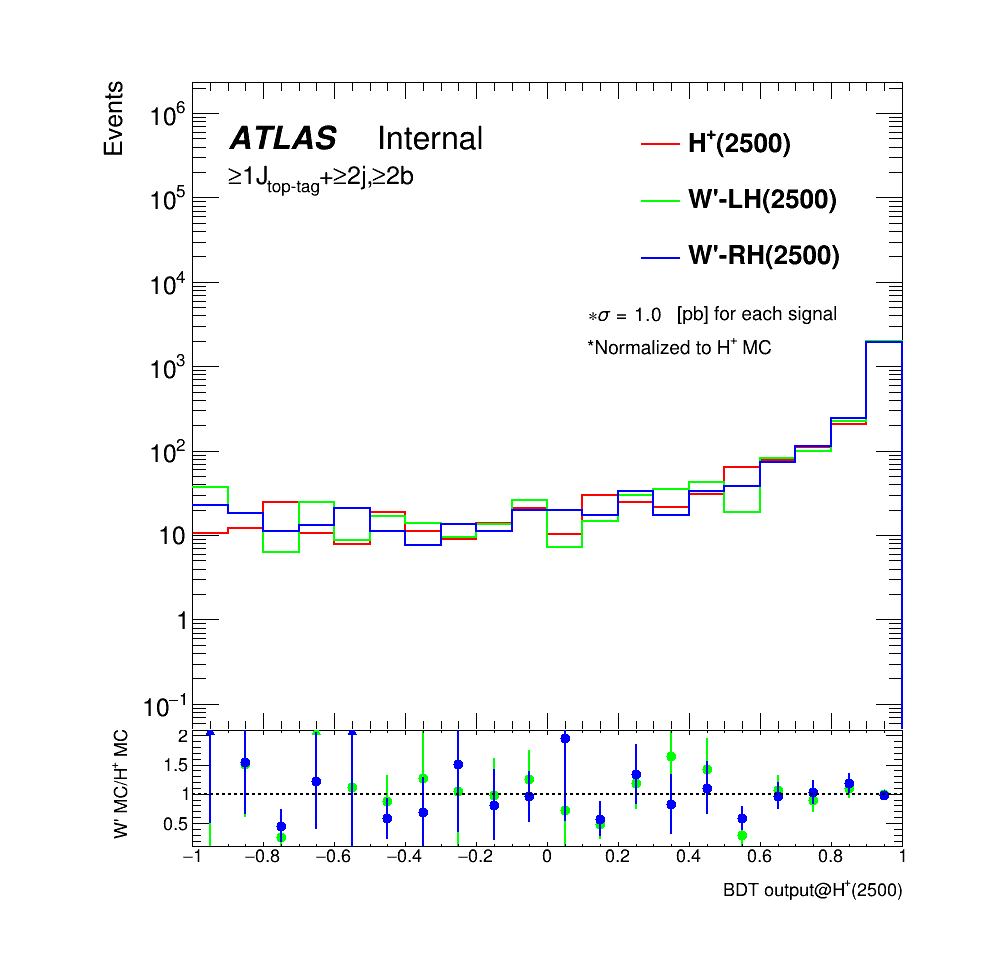
\includegraphics[width=0.45\textwidth]{images/AnalysisStrategy/bdt_Hp2500_2500_geq1tgeq2jgeq2b.png}
            \label{fig:CompHpAndWp_M2500}
        }  
        \subfloat[$M=3.0$ TeV]{
            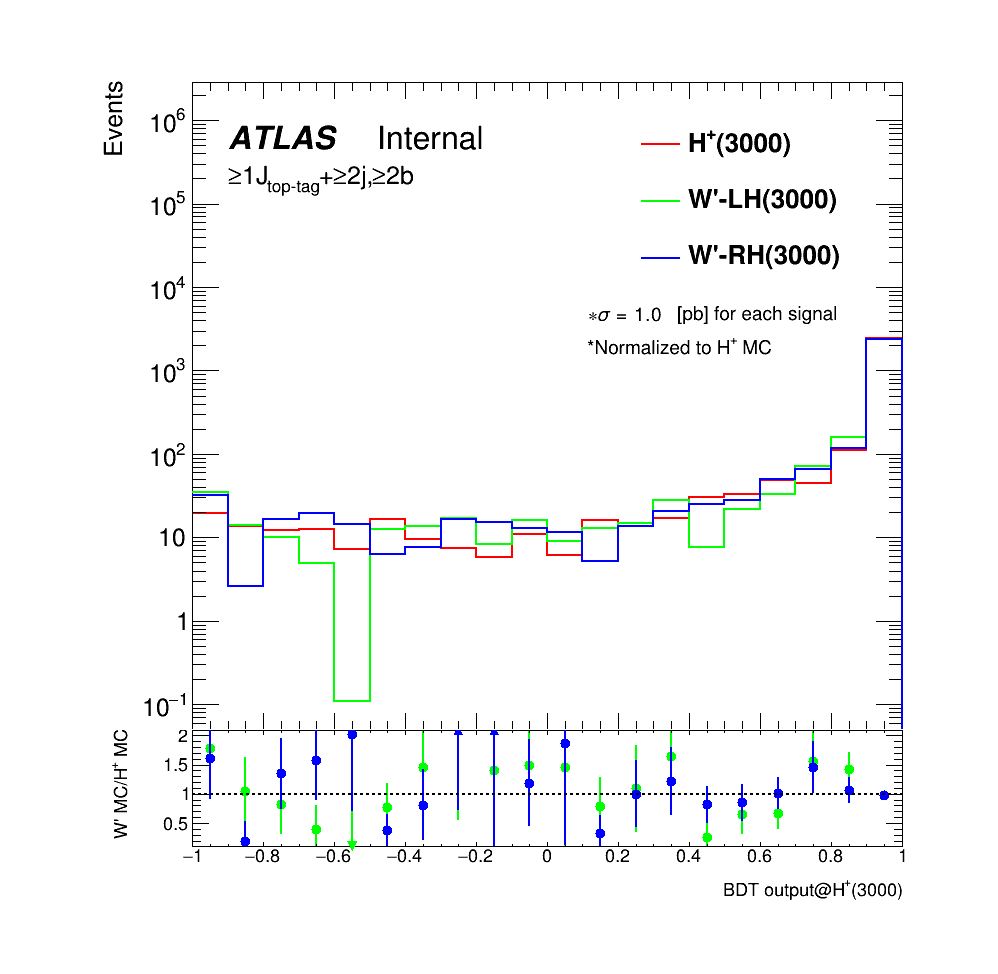
\includegraphics[width=0.45\textwidth]{images/AnalysisStrategy/bdt_Hp3000_3000_geq1tgeq2jgeq2b.png}
            \label{fig:CompHpAndWp_M3000}
        }
        \caption{Comparison of BDT distributions between $H^{+} \rightarrow tb$ and  $W' \rightarrow tb$ events in the SR.}
        \label{fig:CompHpAndWp}
    \end{figure}
    
\end{description}

\subsection{Analysis strategy above 3 TeV}
\label{subsec:AnaStrategyAbove3TeV}
For the mass point above 3 TeV, we adopt a different approach. Since it is difficult to estimate $t\bar{t}+\text{jets}$ events reliably in the very high $H_{\text{T}}^{\text{jets}}$ region where most of the signal events distribute, we use a cut-and-counting method as detailed below, which avoids using the line shapes at the high $H_{\text{T}}^{\text{jets}}$ region, and therefore is more robust against potential mis-modelling compared with the BDT method. 

\begin{figure}[H]
    \subfloat[]{
        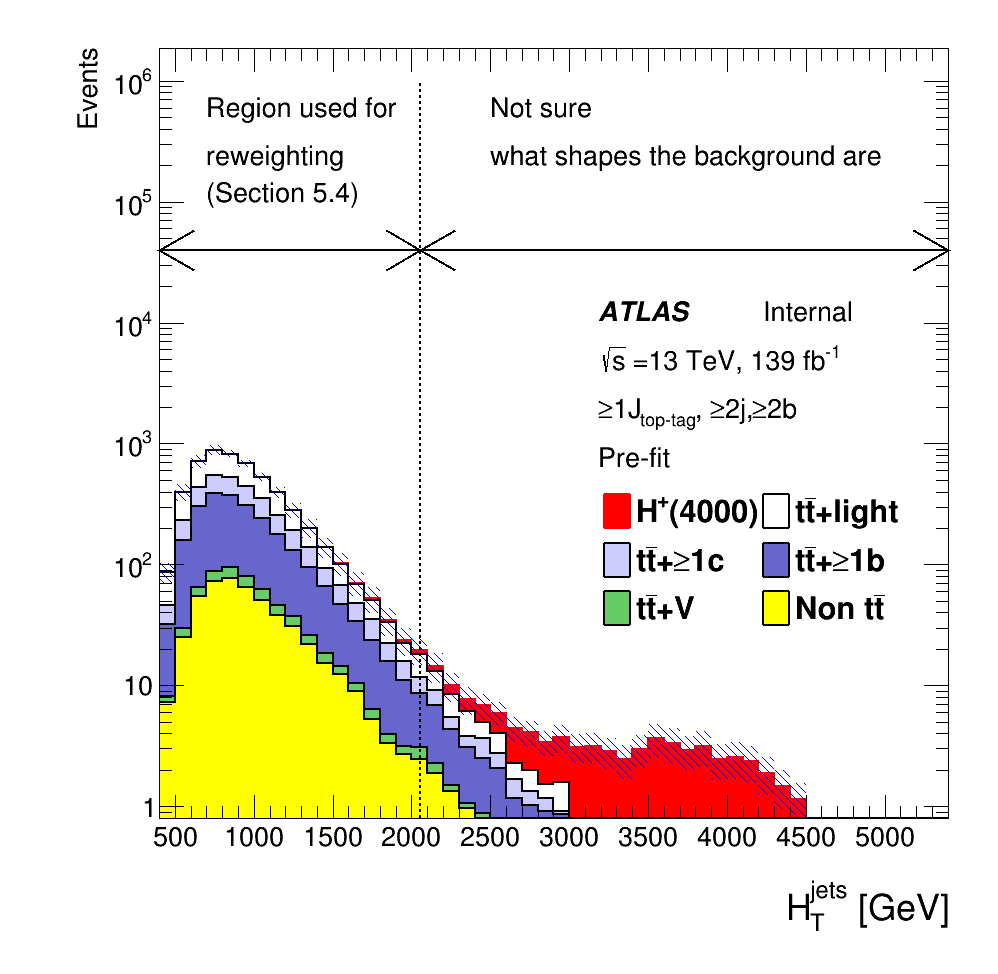
\includegraphics[width=0.45\textwidth]{images/AnalysisStrategy/SOVERB_Hp4000_Contained80_DL1r_70_HTjets_beforeRW_geq1tgeq2jgeq2b_prefit.png}
        \label{fig:SOVERB_HT_jets_4000GeV}
    }
    \subfloat[]{
        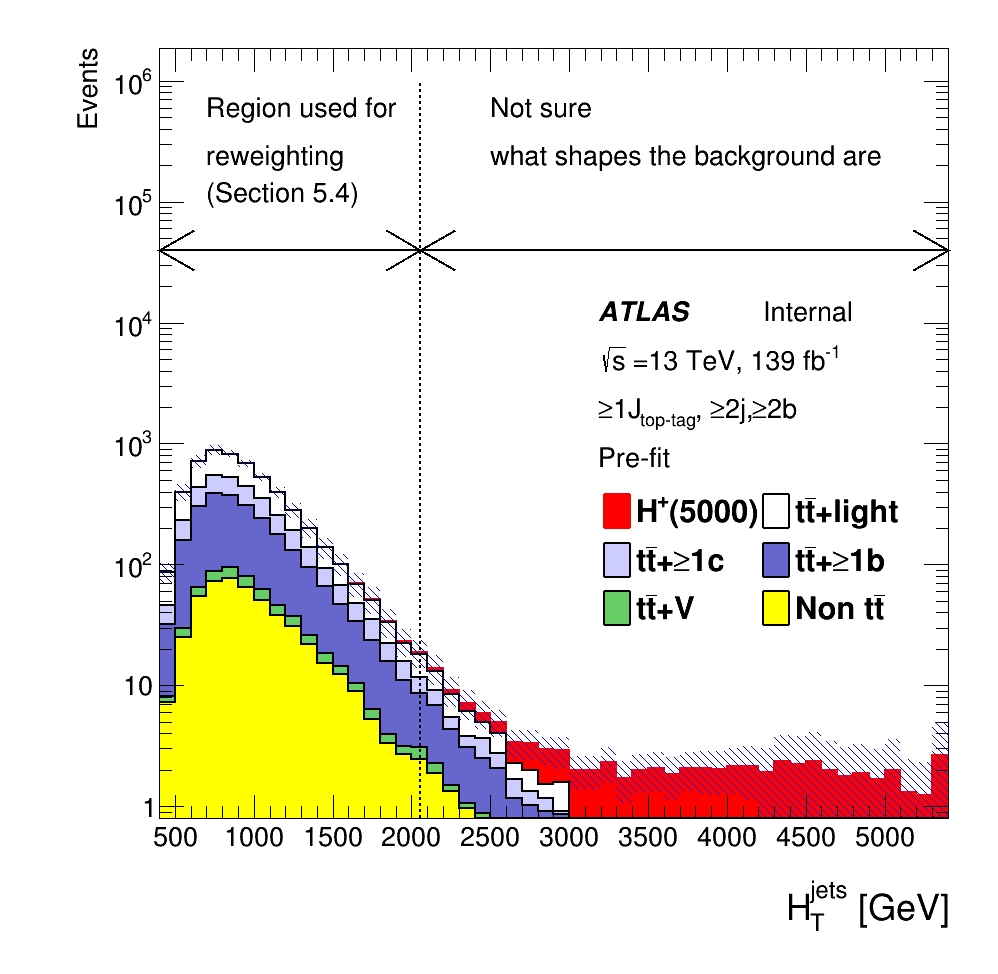
\includegraphics[width=0.45\textwidth]{images/AnalysisStrategy/SOVERB_Hp5000_Contained80_DL1r_70_HTjets_beforeRW_geq1tgeq2jgeq2b_prefit.png}
        \label{fig:SOVERB_HT_jets_5000GeV}
    }
    \caption{Signal and background comparison for 4000 (a) and 5000 (b) GeV mass hypotheses. These signal events distribute mostly in $H_{\text{T}}^{\text{jets}}>2000$ GeV. These regions don't have enough shape information to perform reweighting in Section \ref{subsec:ReweightingTechnique}.}
    \label{fig:SOVERB_HT_jets_4and5TeV}
\end{figure}

One signal region (SR) and two control regions (CR1, CR2) are defined according to the $H_{\text{T}}^{\text{jets}}$ and the number of $b$-jets. Events that have at least two $b$-tagged jets are first required to satisfy the same selection criteria for the SR of the multivariate analysis (Section \ref{subsubsec:RegionDefUnder3TeV}). They are categorized in the SR if they have $H_{\text{T}}^{\text{jets}}>2000$ GeV, while events with $H_{\text{T}}^{\text{jets}} \leq 2000$ are categorized into the CR1, depending on $\text{N}_{b_{\text{jets}}}$. All events that have exactly one $b$-tagged jet are categorized into CR2, which is the same as the CR of the multivariate analysis. The event selections in these regions are summarized in Table \ref{tab:EventSelectionInSRAndCR1AndCR2}. Figure \ref{fig:BkgComposition_SR_CC} to \ref{fig:BkgComposition_CR2_CC} shows the background compositions in each region. $H_{\text{T}}^{\text{jets}}$ is used as final discriminates, as discussed in Section \ref{sec:ProfileLikelohoodFit}. The number of bins of $H_{\text{T}}^{\text{jets}}$ distribution in the SR is set to one. The CR1 and CR2 are enriched in $t\bar{t}+\text{light}$ and $t\bar{t}+\text{HF}$ events, respectively. Therefore, these regions are used to control $t\bar{t}+\text{jets}$ events in the final fittings. 

\begin{table}[H]
    \centering
    \begin{tabular*}{130mm}{c|c|c|c}
        \hline\hline
        Cut                          & SR & CR1 & CR2\\
        \hline
        leptons                      & \multicolumn{3}{c}{Same requirements as Table \ref{tab:EventSelectionInSR1AndSR2}}\\
        \hline
        Top-tagged large-$R$ jets    & \multicolumn{3}{c}{Same requirements as Table \ref{tab:EventSelectionInSR1AndSR2}}\\
        \hline
        Small-$R$ jets               & \multicolumn{2}{c|}{$\text{N}_{\text{jet}} \geq 2$}    & $\text{N}_{\text{jet}} \geq 1$ \\
                                     & \multicolumn{2}{c|}{(Kinematic requirements}  & (Kinematic requirements \\
                                     & \multicolumn{2}{c|}{are the same as Table \ref{tab:EventSelectionInSR1AndSR2})} & are the same as Table \ref{tab:EventSelectionInSR1AndSR2})\\
        \hline
        $b$-tagged small-$R$ jets    & \multicolumn{2}{c|}{$\text{N}_{b-\text{jet}} \geq 2$}  & $\text{N}_{b-\text{jet}} = 1$\\
        \hline
        $H_{\text{T}}^{\text{jets}}$ & $> 2000$ GeV & $\leq 2000$ GeV & No cut\\
        \hline\hline
  \end{tabular*}
  \caption{Event selections in the SR, CR1, and CR2. After these selections, CR1 becomes enriched in $t\bar{t}+\text{light}$, and CR2 becomes enriched in $t\bar{t}+\text{HF}$.}
  \label{tab:EventSelectionInSRAndCR1AndCR2}
\end{table}

%--- Figure for SR
\begin{figure}[H]
  \centering
  \subfloat[]{
    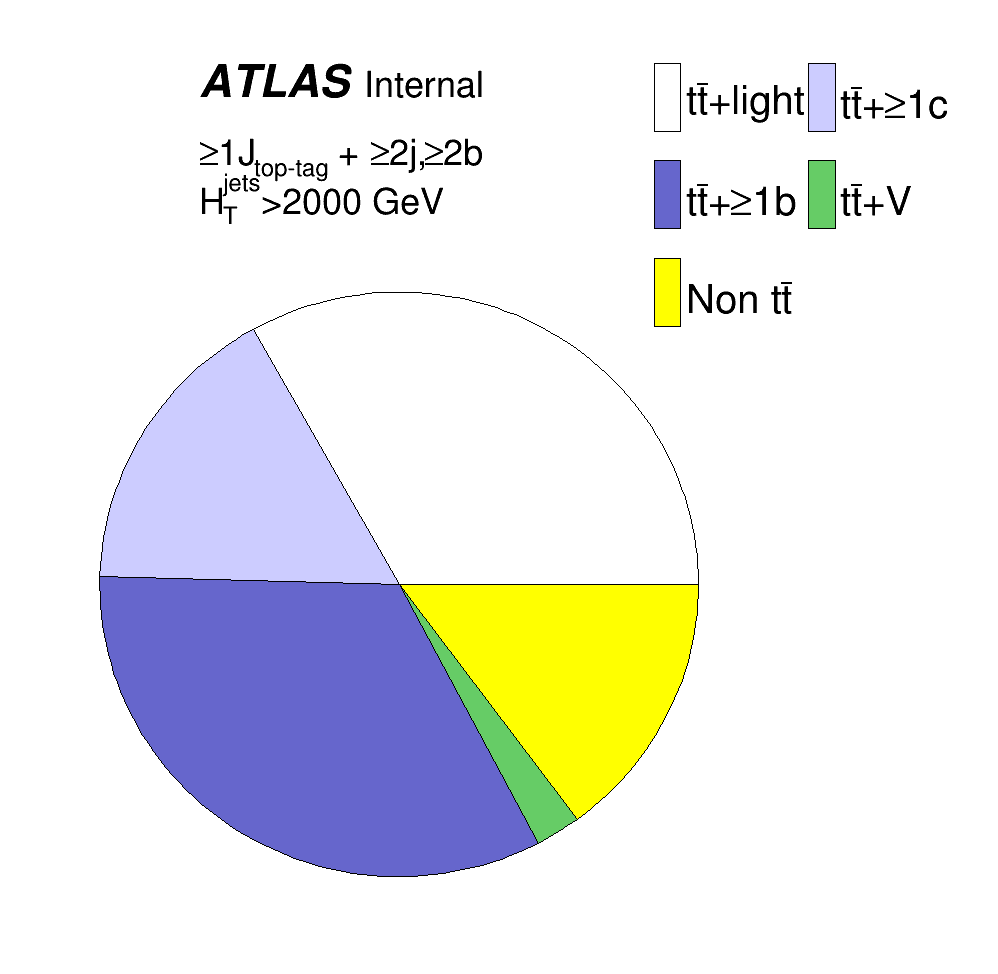
\includegraphics[keepaspectratio,scale=0.2]{images/AnalysisStrategy/PieChart_SR_CC.png}
    \label{fig:PieChart_SR_CC}
  }
  \subfloat[]{
    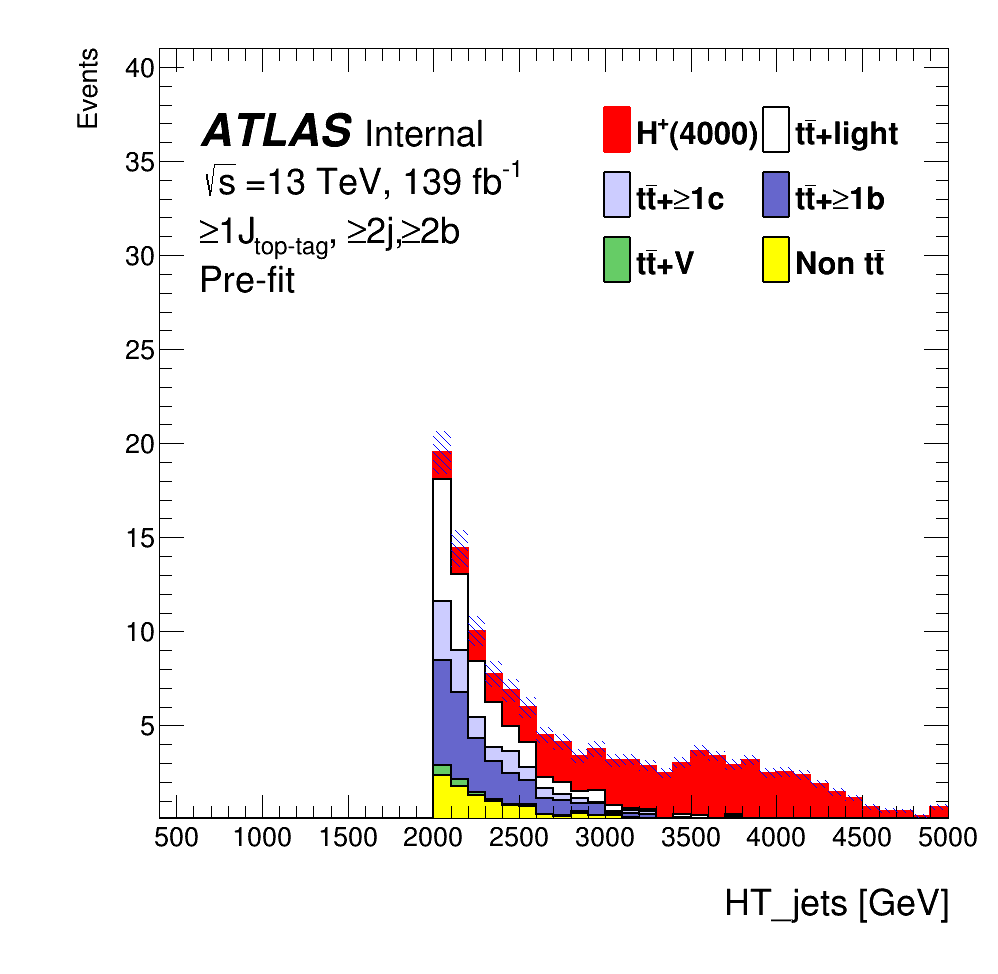
\includegraphics[keepaspectratio,scale=0.2]{images/AnalysisStrategy/HTjets_SR_CC.png}
    \label{fig:PieChart_SR1}
  }
  \caption{Background composition in the SR is shown in the pie chart (a) and the $H_{\text{T}}^{\text{jets}}$ distributions (b). The number of bins of $H_{\text{T}}^{\text{jets}}$ distribution is set to exactly one.}
  \label{fig:BkgComposition_SR_CC}
\end{figure}

%--- Figure for CR1
\begin{figure}[H]
  \centering
  \subfloat[]{
    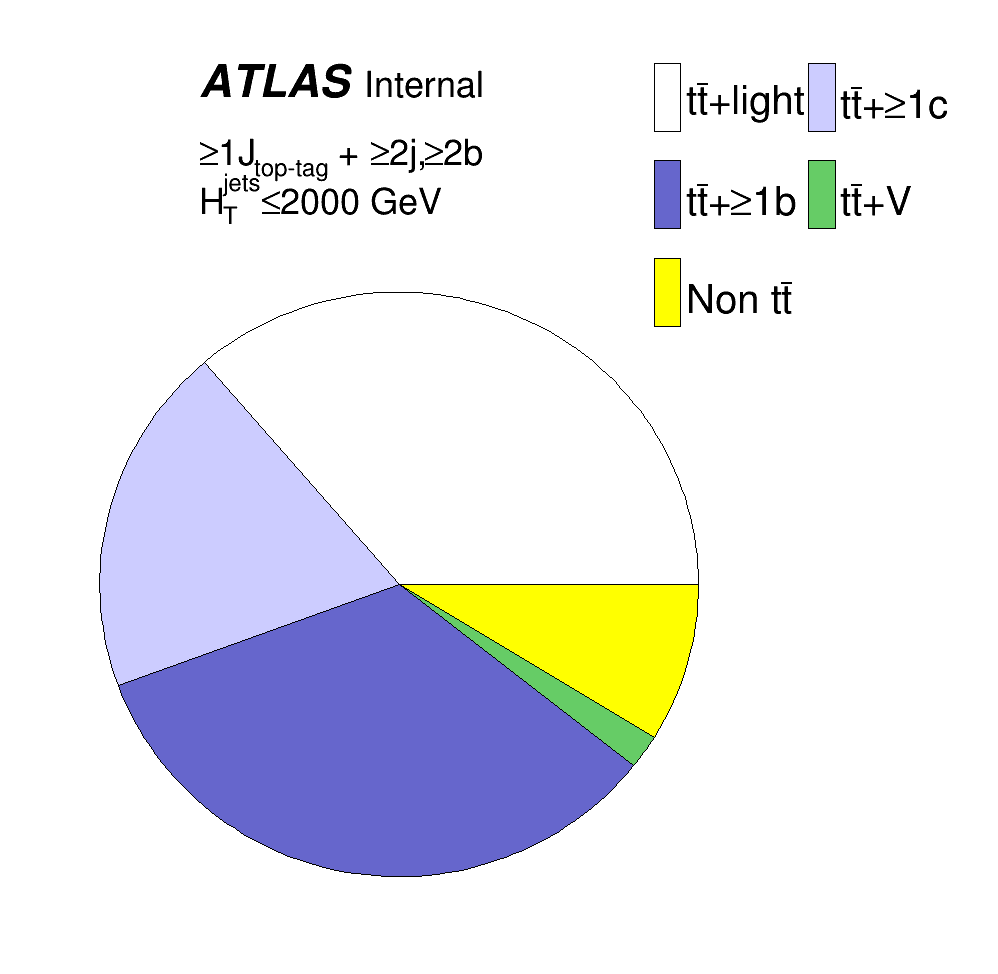
\includegraphics[keepaspectratio,scale=0.2]{images/AnalysisStrategy/PieChart_CR1_CC.png}
    \label{fig:PieChart_CR1}
  }
  \subfloat[]{
    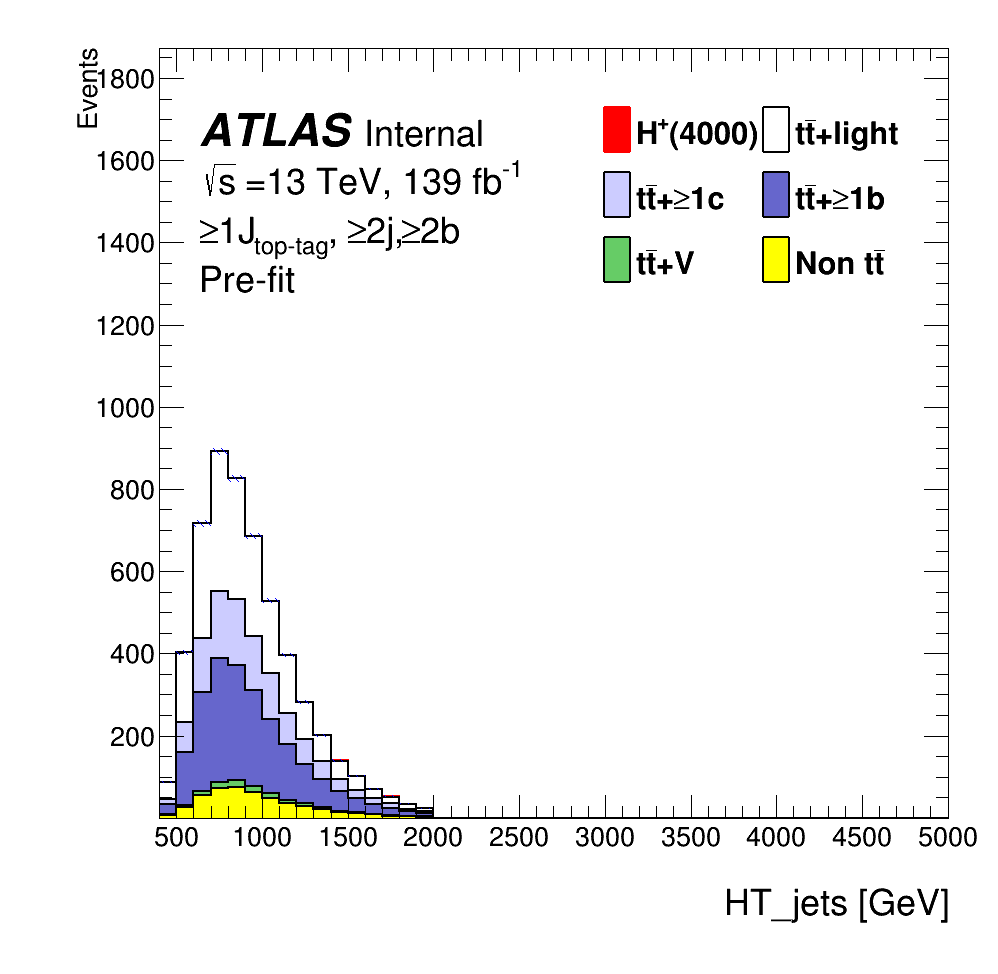
\includegraphics[keepaspectratio,scale=0.2]{images/AnalysisStrategy/HTjets_CR1_CC.png}
    \label{fig:PieChart_CR1}
  }
  \caption{Background composition in the CR1 is shown in the pie chart (a) and the $H_{\text{T}}^{\text{jets}}$ distributions (b).}
  \label{fig:BkgComposition_CR1_CC}
\end{figure}

%--- Figure for CR1
\begin{figure}[H]
  \centering
  \subfloat[]{
    \includegraphics[keepaspectratio,scale=0.2]{images/AnalysisStrategy/PieChart_CR2_CC.png}
    \label{fig:PieChart_CR2}
  }
  \subfloat[]{
    \includegraphics[keepaspectratio,scale=0.2]{images/AnalysisStrategy/HTjets_CR2_CC.png}
    \label{fig:PieChart_CR2}
  }
  \caption{Background composition in the CR2 is shown in the pie chart (a) and the $H_{\text{T}}^{\text{jets}}$ distributions (b). The CR2 is the same region as the CR of multivariate analysis defined in Section \ref{subsubsec:RegionDefUnder3TeV}.}
  \label{fig:BkgComposition_CR2_CC}
\end{figure}

The number of expected signal and background events in the SR, CR1, and CR2 are shown in Table \ref{tab:PrefitYieldsAbove3TeV}. The predicted number of $H^{+}$ and $W'$ signal events for the 4000 and 5000 GeV mass hypothesis are estimated using $\sigma \times Br = 0.046$ pb, as done in Table \ref{tab:PrefitYields}.

\begin{table}[H]
  \centering
  \begin{tabular*}{130mm}{@{\extracolsep{\fill}}cccc}
    \hline\hline
                            & SR           & CR1             & CR2\\
    \hline
    $t\bar{t}+\text{light}$ & $21 \pm  3$  & $1920 \pm 162$  & $ 34 \pm  5$\\
    $t\bar{t}+\geq1c$       & $11 \pm  9$  & $1007 \pm 782$  & $ 39 \pm 37$\\
    $t\bar{t}+\geq1b$       & $21 \pm 10$  & $1568 \pm 794$  & $249 \pm 46$\\
    $t\bar{t}+W$            & $ 1 \pm  0$  & $  35 \pm   6$  & $  2 \pm  0$\\
    $t\bar{t}+Z$            & $ 1 \pm  0$  & $  57 \pm   8$  & $  9 \pm  2$\\
    $Wt$ channel            & $ 3 \pm  3$  & $ 173 \pm 101$  & $  7 \pm  4$\\
    $t$ channel             & $ 1 \pm  0$  & $  35 \pm  16$  & $ 16 \pm  1$\\
    Other top sources       & $ 1 \pm  0$  & $  28 \pm  12$  & $  8 \pm  4$\\
    $VV$, $V$+jets          & $ 5 \pm  2$  & $ 132 \pm  53$  & $  4 \pm  2$\\
    $t\bar{t}H$             & $ 1 \pm  0$  & $  78 \pm   3$  & $ 24 \pm  1$\\
    \hline
    Total                   & $65 \pm  7$  & $5033 \pm 308$  & $377 \pm 33$\\
    \hline
    $H^{+}$ 4000 GeV        & $57 \pm 18$  & $   5 \pm   2$  & $  2 \pm  0$\\
    $H^{+}$ 5000 GeV        & $55 \pm 27$  & $   3 \pm   1$  & $  1 \pm  0$\\
    \hline\hline
  \end{tabular*}
  \caption{Number of expected and selected events split according to the SR, CR1, and CR2. The quoted uncertainties include both statistical and systematic uncertainties before fitting.}
  \label{tab:PrefitYieldsAbove3TeV}
\end{table}
\clearpage
%----------------------------------------------------------------------

%----------------------------------------------------------------------
\section{Background modeling}
\label{sec:BkgModeling}

\subsection{Blind strategy}
\label{subsec:BlindStrategy}
In the following sections, the modelling of kinematic distributions, particularly those used for BDT training, of the $t\bar{t}+\text{jets}$ background is checked by comparing the data and MC. In order to avoid observing signals or any other biases before fixing the analysis procedure, the following blinding strategy is applied. The signal-to-noise ratio ($S/B$) is calculated in each bin of each distribution for all mass hypotheses (more details in Appendix \ref{app:SignalBackgroundComparison}). The signal cross section (${\sigma}_{\text{signal}}$) on each mass hypothesis is set to 0.046 pb, which is the upper limit at 1 TeV $H^{+}$ mass point obtained from the resolved $H^{+}{\rightarrow}tb$ search \cite{HDBS-2021-02}. Therefore, it can be considered the most conservative assumption. The data in bins with $S/B>0.05$ in at least one mass hypothesis are blinded when the data is compared with MC.

\subsection{Data/MC comparison for BDT input variables}
\label{subsec:Data/MCBDTInputBeforeReweight}
Figures \ref{fig:DATAOVERMC_BDTInputs_Prefit} show the distributions of input variables for BDT training in the SR region with all systematic uncertainty sources, which are summarised in Table \ref{tab:SystSources}, except for $t\bar{t}+\text{jets}$ reweighting source. Data are blinded according to the blind strategy in Section \ref{subsec:BlindStrategy}. No significant difference between the data and MC is found in each variable.

\begin{figure}[H]
    \subfloat[HT\_jets] {
        \includegraphics[width=0.50\textwidth]{images/BkgModeling/DATAOVERMC_Hp1000_Contained80_DL1r_70_HTjets_beforeRW_geq1tgeq2jgeq2b_prefit.png}
        \label{fig:DATAOVERMC_HT_jets}
    }
    \subfloat[LeadingJet\_pt] {
        \includegraphics[width=0.50\textwidth]{images/BkgModeling/DATAOVERMC_Hp1000_Contained80_DL1r_70_LeadingJet_pt_beforeRW_geq1tgeq2jgeq2b_prefit.png}
        \label{fig:DATAOVERMC_LeadingJet_pt}
    }
\end{figure}
\begin{figure}[H]
    %\addtocounter{figure}{-1}
    \subfloat[Centrality\_all] {
        \includegraphics[width=0.50\textwidth]{images/BkgModeling/DATAOVERMC_Hp1000_Contained80_DL1r_70_Centrality_all_beforeRW_geq1tgeq2jgeq2b_prefit.png}
        \label{fig:DATAOVERMC_Centrality_all}
    }
    \subfloat[H1\_all] {
        \includegraphics[width=0.50\textwidth]{images/BkgModeling/DATAOVERMC_Hp1000_Contained80_DL1r_70_H1_all_beforeRW_geq1tgeq2jgeq2b_prefit.png}
        \label{fig:DATAOVERMC_H1_all}
    }
\end{figure}
\begin{figure}[H]
    %\addtocounter{figure}{-1}
    \subfloat[Mbb\_MaxPt] {
        \includegraphics[width=0.50\textwidth]{images/BkgModeling/DATAOVERMC_Hp1000_Contained80_DL1r_70_Mbb_MaxPt_beforeRW_geq1tgeq2jgeq2b_prefit.png}
        \label{fig:DATAOVERMC_Mbb_MaxPt}
    }
    \subfloat[Mjjj\_MaxPt] {
        \includegraphics[width=0.50\textwidth]{images/BkgModeling/DATAOVERMC_Hp1000_Contained80_DL1r_70_Mjjj_MaxPt_beforeRW_geq1tgeq2jgeq2b_prefit.png}
        \label{fig:DATAOVERMC_Mjjj_MaxPt}
    }
\end{figure}
\begin{figure}[H]
    %\addtocounter{figure}{-1}
    \subfloat[Muu\_MindR] {
        \includegraphics[width=0.50\textwidth]{images/BkgModeling/DATAOVERMC_Hp1000_Contained80_DL1r_70_Muu_MindR_beforeRW_geq1tgeq2jgeq2b_prefit.png}
        \label{fig:DATAOVERMC_Muu_MindR}
    }
    \subfloat[dRbb\_avg] {
        \includegraphics[width=0.50\textwidth]{images/BkgModeling/DATAOVERMC_Hp1000_Contained80_DL1r_70_dRbb_avg_beforeRW_geq1tgeq2jgeq2b_prefit.png}
        \label{fig:DATAOVERMC_dRbb_avg}
    }
\end{figure}
\begin{figure}[H]
    %\addtocounter{figure}{-1}
    \subfloat[dRlepbb\_MindR] {
        \includegraphics[width=0.50\textwidth]{images/BkgModeling/DATAOVERMC_Hp1000_Contained80_DL1r_70_dRlepbb_MindR_beforeRW_geq1tgeq2jgeq2b_prefit.png}
        \label{fig:DATAOVERMC_dRlepbb_MindR}
    }
    \subfloat[LeadingTop\_m] {
        \includegraphics[width=0.50\textwidth]{images/BkgModeling/DATAOVERMC_Hp1000_Contained80_DL1r_70_LeadingTop_mass_beforeRW_geq1tgeq2jgeq2b_prefit.png}
        \label{fig:DATAOVERMC_LeadingTop_mass}
    }
\end{figure}
\begin{figure}[H]
    %\addtocounter{figure}{-1}
    \subfloat[LeadingTop\_pt] {
        \includegraphics[width=0.50\textwidth]{images/BkgModeling/DATAOVERMC_Hp1000_Contained80_DL1r_70_LeadingTop_pt_beforeRW_geq1tgeq2jgeq2b_prefit.png}
        \label{fig:DATAOVERMC_LeadingTop_pt}
    }
    \subfloat[M\_tb] {
        \includegraphics[width=0.50\textwidth]{images/BkgModeling/DATAOVERMC_Hp1000_Contained80_DL1r_70_tb_mass_beforeRW_geq1tgeq2jgeq2b_prefit.png}
        \label{fig:DATAOVERMC_tb_mass}
    }
\end{figure}
\begin{figure}[H]
    %\addtocounter{figure}{-1}
    \subfloat[Pt\_tb] {
        \includegraphics[width=0.50\textwidth]{images/BkgModeling/DATAOVERMC_Hp1000_Contained80_DL1r_70_tb_pt_beforeRW_geq1tgeq2jgeq2b_prefit.png}
        \label{fig:DATAOVERMC_tb_pt}
    }
    \subfloat[PtAsymm\_tb] {
        \includegraphics[width=0.50\textwidth]{images/BkgModeling/DATAOVERMC_Hp1000_Contained80_DL1r_70_tb_ptAsymm_beforeRW_geq1tgeq2jgeq2b_prefit.png}
        \label{fig:DATAOVERMC_tb_ptAsymm}
    }
  \caption{Comparison of the kinematic variables included in the BDT in the SR for the data and MC with all systematics uncertainties, which are summarised in Table \ref{tab:SystSources}, except for $t\bar{t}+\text{jets}$ reweighting source.}
  \label{fig:DATAOVERMC_BDTInputs_Prefit}
\end{figure}


\subsection{Data/MC comparison for BDT outputs}
\label{subsec:DataAndMCComparisonOfBDT}
Figures \ref{fig:DataMCComparison_BDT_Hp1000_SR_beforeRW} to \ref{fig:DataMCComparison_BDT_Hp3000_SR_beforeRW} show the distributions of BDT output in the SR. The binning of each BDT output is optimized for the search sensitivity by \textit{TransfoD} algorithm \cite{Binning-TTHFilter}. Such binning results in extremely narrow bins towards high BDT scored and makes the plot hard to see, as shown in Figure \ref{fig:SOVERB_bdt_beforeRW_geq1tgeq2jgeq2b} in Appendix \ref{subapp:SOVERB_BDTOutput} when plotted in a usual manner. We rather show the distribution with an equal interval for each bin. The distributions are input into the profile likelihood fit on each $H^{+}$ mass hypothesis as shown in Section \ref{sec:ProfileLikelohoodFit}. It is observed that the data/MC ratio tends to be lower for the high BDT score regions, which may bias the search for the signal in the highest BDT bins. The reweighting to correct for the slope is discussed in Section \ref{subsec:ReweightingTechnique}. 

\begin{figure}[H]
    \subfloat[] {
        \includegraphics[width=0.50\textwidth]{images/BkgModeling/DATAOVERMC_Hp1000_Contained80_DL1r_70_bdt_Hp1000_beforeRW_geq1tgeq2jgeq2b_prefit.png}
        \label{fig:DataMCComparison_BDT_Hp1000_SR_beforeRW}
    }
    \subfloat[] {
        \includegraphics[width=0.50\textwidth]{images/BkgModeling/DATAOVERMC_Hp1200_Contained80_DL1r_70_bdt_Hp1200_beforeRW_geq1tgeq2jgeq2b_prefit.png}
        \label{fig:DataMCComparison_BDT_Hp1200_SR_beforeRW}
    }\par
    \subfloat[] {
        \includegraphics[width=0.50\textwidth]{images/BkgModeling/DATAOVERMC_Hp1400_Contained80_DL1r_70_bdt_Hp1400_beforeRW_geq1tgeq2jgeq2b_prefit.png}
        \label{fig:DataMCComparison_BDT_Hp1400_SR_beforeRW}
    }
    \subfloat[] {
        \includegraphics[width=0.50\textwidth]{images/BkgModeling/DATAOVERMC_Hp1600_Contained80_DL1r_70_bdt_Hp1600_beforeRW_geq1tgeq2jgeq2b_prefit.png}
        \label{fig:DataMCComparison_BDT_Hp1600_SR_beforeRW}
    }
\end{figure}
\begin{figure}[H]
    %\addtocounter{figure}{-1}
    \subfloat[] {
        \includegraphics[width=0.50\textwidth]{images/BkgModeling/DATAOVERMC_Hp1800_Contained80_DL1r_70_bdt_Hp1800_beforeRW_geq1tgeq2jgeq2b_prefit.png}
        \label{fig:DataMCComparison_BDT_Hp1800_SR_beforeRW}
    }
    \subfloat[] {
        \includegraphics[width=0.50\textwidth]{images/BkgModeling/DATAOVERMC_Hp2000_Contained80_DL1r_70_bdt_Hp2000_beforeRW_geq1tgeq2jgeq2b_prefit.png}
        \label{fig:DataMCComparison_BDT_Hp2000_SR_beforeRW}
    }\par
    \subfloat[] {
        \includegraphics[width=0.50\textwidth]{images/BkgModeling/DATAOVERMC_Hp2500_Contained80_DL1r_70_bdt_Hp2500_beforeRW_geq1tgeq2jgeq2b_prefit.png}
        \label{fig:DataMCComparison_BDT_Hp2500_SR_beforeRW}
    }
    \subfloat[] {
        \includegraphics[width=0.50\textwidth]{images/BkgModeling/DATAOVERMC_Hp3000_Contained80_DL1r_70_bdt_Hp3000_beforeRW_geq1tgeq2jgeq2b_prefit.png}
        \label{fig:DataMCComparison_BDT_Hp3000_SR_beforeRW}
    }
    \caption{Pre-fit distribution of BDT output trained using from 1000 GeV (a) to 3000 GeV (h) $H^{+}$ samples in the SR.}
    \label{fig:DataMCComparison_BDT_beforeRW}
\end{figure}

\subsection{Reweighting technique}
\label{subsec:ReweightingTechnique}
Due to the mismodeling of the hard and soft jets, some extent of mis-modelling is expected in the $t\Bar{t}+\text{jets}$ samples generated by Powheg + Phytia. These mis-modelings appear, for example, in the number of jets, $p_\text{T}$ distribution of the leading top-tagged large-R jet (LeadingTop\_pt) and the invariant mass distribution of small-R jet triplet with maximum $p_{\text{T}}$ (Mjjj\_MaxPt) (these small-R jets are mainly QCD jets) as shown in Figure \ref{fig:DataMCComparison_In_LowBDTSocreRegion}.

\begin{figure}[H]
    \centering
    \subfloat[] {
        \includegraphics[width=0.50\textwidth]{images/BkgModeling/DATAOVERMC_Hp1000_Contained80_DL1r_70_nJets_beforeRW_geq1tgeq1j1b_prefit.png}
        \label{fig:nJets_CR}
    }\par
    \subfloat[] {
        \includegraphics[width=0.50\textwidth]{images/BkgModeling/DATAOVERMC_Hp1000_Contained80_DL1r_70_LeadingTop_pt_LowBDTScore_beforeRW_geq1tgeq2jgeq2b_prefit.png}
        \label{fig:LeadingTop_pt_Modeling_LowBDTScoreEvents}
    }
    \subfloat[] {
        \includegraphics[width=0.50\textwidth]{images/BkgModeling/DATAOVERMC_Hp1000_Contained80_DL1r_70_Mjjj_MaxPt_LowBDTScore_beforeRW_geq1tgeq2jgeq2b_prefit.png}
        \label{fig:Mjjj_MaxPt_Modeling_LowBDTScoreEvents}
    }
    \caption{Number of jets in the CR (a), $p_{\text{T}}$ distribution of the leading top-tagged large-R jet in the SR (b) and invariant mass distribution of small-R jet triplet with maximum $p_{\text{T}}$ in the SR (c). These events in the SR are required to pass all BDT cuts shown in Table \ref{tab:ReqForRWControlRegion}. Each data/MC ratio plot has a slope.}
    \label{fig:DataMCComparison_In_LowBDTSocreRegion}
\end{figure}


To improve the prediction of $t\bar{t}+\text{jets}$, data-based corrections are applied to the MC prediction. The reweighing factors are derived by comparing the number of jets ($\text{N}_{\text{jets}}$) and $H_{\text{T}}^{\text{jets}}$ distributions between data and MC prediction. The reweighting factors for $\text{N}_{\text{jets}}$ are derived in the CR. Since the modelling is assumed to be due mainly to the additional radiation in the parton shower, which is independent on the flavour of associated jets, these reweighting factors are expected to improve the data/MC agreement in the SR as well, to the point that the remaining discrepancies would be well covered by the systematic model. The reweighting factors for $H_{\text{T}}^{\text{jets}}$ are derived in the SR and CR, individually, after reweighting with $\text{N}_{\text{jets}}$. When the reweighting factors are derived in the SR, events in the only low BDT score region are selected to avoid being reweighted signal events. These events are required to pass all the cuts shown in Table \ref{tab:ReqForRWControlRegion}. 

Firstly, the data/MC ratios $R$ are derived according to the following definition:
\begin{equation}
  R = \frac{\text{Data}-\text{MC}^{\text{non-}t\bar{t}+\text{jets}}}{f \cdot \text{MC}^{t\bar{t}+\text{jets}}}
\end{equation}

$t\bar{t}+\text{jets}$ includes the $t\bar{t}+\text{light}$, $t\bar{t}+\geq1c$ and $t\bar{t}+\geq1b$. The number of $t\bar{t}+\text{jets}$ MC events is scaled by $f$ to the number of data subtracted non $t\bar{t}+\text{jets}$ MC events. Figure \ref{fig:RWFactors_Njets_CR} shows the number of jets and data/MC ratio, $R$, distributions. The first reweighting is performed using the $R$ in each $\text{N}_{\text{jets}}$ bin, which is applied to $t\bar{t}+\text{light}$, $t\bar{t}+\geq1c$ and $t\bar{t}+\geq1b$. Figure \ref{fig:RWFactors_HTjets} shows the $H_{\text{T}}^{\text{jets}}$ and $R$ distributions in each SR and CR after reweighting with $\text{N}_{\text{jets}}$. When the $R$ is derived in the SR, events in the only low BDT score region are selected to avoid being reweighted signal events according to Table \ref{tab:ReqForRWControlRegion}. These obtained $R$ distributions are fitted with a quadratic function ($f(H_{\text{T}}^{\text{jets}}) = a + b \cdot H_{\text{T}}^{\text{jets}} + c \cdot (H_{\text{T}}^{\text{jets}})^{2}$, where $a$, $b$, and $c$ are free parameters determined in the fit), and the function is used for reweighting. The function is applied to $t\bar{t}+\text{light}$, $t\bar{t}+\geq1c$ and $t\bar{t}+\geq1b$ as well as $\text{N}_{\text{jets}}$ reweighting. The obtained reweighting functions are also shown in Figure \ref{fig:RWFactors_HTjets}. Table \ref{tab:ParameterOfReweightingFunction} includes the fitted values for all the parameters. The statistical errors of fitted parameters are included as systematic uncertainties in the final fitting. The reweighting factors in $H_{\text{T}}^{\text{jets}}>2072$ GeV region are used the value at $H_{\text{T}}^{\text{jets}}=2072$ GeV because the weight value of $-1\sigma$ become negative at the point.

\begin{table}[H]
  \centering
  \begin{tabular*}{70mm}{@{\extracolsep{\fill}}cc}
    \hline\hline
    Mass point [GeV] & BDT score cut\\
    \hline
    1000             & $< 0.5$\\
    1200             & $< 0.5$\\
    1400             & $< 0.5$\\
    1600             & $< 0.5$\\
    1800             & $< 0.5$\\
    2000             & $< 0.5$\\
    2500             & $< 0.5$\\
    3000             & $<-0.2$\\
    4000             & $<-0.2$\\
    5000             & $<-0.2$\\
    \hline\hline
  \end{tabular*}
  \caption{Requirements on the events used for reweighting factor calculation in the SR. These cuts are defined so that events are derived from the regions with S/B $<$ 0.05 for any mass points.}
  \label{tab:ReqForRWControlRegion}
\end{table}

\begin{figure}[H]
    \centering
    \includegraphics[width=0.50\textwidth]{images/BkgModeling/RWFactors_Njets.png}
    \caption{Number of jets (top canvas) and data/MC ratio, $R$, (bottom canvas) distributions. The first reweighting is performed using the $R$ in each $\text{N}_{\text{jets}}$ bin, , which is applied to $t\bar{t}+\text{light}$, $t\bar{t}+\geq1c$ and $t\bar{t}+\geq1b$.}
    \label{fig:RWFactors_Njets_CR}
\end{figure}

\begin{figure}[H]
  \subfloat[] {
    \includegraphics[width=0.50\textwidth]{images/BkgModeling/RWFactors_HTjets_SR.png}
    \label{fig:HTjets_LowBDTScoreRegion}
  }
  \subfloat[] {
    \includegraphics[width=0.50\textwidth]{images/BkgModeling/RWFactors_HTjets_CR.png}
    \label{fig:HTjets_WeightFactor}
  }
  \caption{$H_{\text{T}}^{\text{jets}}$ and data/MC ratio, $R$, distributions in the SR (a) and CR (b). The events in the SR are selected by BDT score. The red functions in the bottom canvases are the reweighting functions obtained by fitting to $R$ distribution with a quadratic function. The blue bands are the statistical uncertainty (${\pm}1{\sigma}$) of the red function. They are included as systematic uncertainties in the final fitting. For events with $H_{\text{T}}^{\text{jets}}>2072$ GeV in the SR, the same weight and its error as region $H_{\text{T}}^{\text{jets}}=2072$ GeV is given. }
  \label{fig:RWFactors_HTjets}
\end{figure}


\begin{table}[H]
  \centering
  \begin{tabular*}{120mm}{c|c|c}
    \hline\hline
    Parameter & Value (SR)                      & Value (CR)\\
    \hline
    $a$       & $( 7.95{\pm}1.45)\times10^{-1}$ & $( 9.20{\pm}0.32)\times10^{-1}$\\
    \hline
    $b$       & $( 6.70{\pm}2.82)\times10^{-4}$ & $( 2.14{\pm}0.67)\times10^{-4}$\\
    \hline
    $c$       & $(-4.75{\pm}1.29)\times10^{-7}$ & $(-1.29{\pm}0.32)\times10^{-7}$\\
    \hline\hline
  \end{tabular*}
  \caption{Summary of parameters obtained by fitting of a quadratic function in the SR and CR ($f(H_{\text{T}}^{\text{jets}}) = a + b \cdot H_{\text{T}}^{\text{jets}} + c \cdot (H_{\text{T}}^{\text{jets}})^{2}$). The error of each parameter is from statistical uncertainty.}
  \label{tab:ParameterOfReweightingFunction}
\end{table}


Figure \ref{fig:BDT_Hp1000_AfterRW} to Figure \ref{fig:BDT_Hp3000_AfterRW} show BDT output distributions applied to reweighting in the SR. The data/MC agreement in the high BDT score regions is improved.

\begin{figure}[H]
    \subfloat[] {
        \includegraphics[width=0.50\textwidth]{images/BkgModeling/DATAOVERMC_Hp1000_Contained80_DL1r_70_bdt_Hp1000_geq1tgeq2jgeq2b_prefit.png}
        \label{fig:BDT_Hp1000_AfterRW}
    }
    \subfloat[] {
        \includegraphics[width=0.50\textwidth]{images/BkgModeling/DATAOVERMC_Hp1200_Contained80_DL1r_70_bdt_Hp1200_geq1tgeq2jgeq2b_prefit.png}
        \label{fig:BDT_Hp1200_AfterRW}
    }\par
    \subfloat[] {
        \includegraphics[width=0.50\textwidth]{images/BkgModeling/DATAOVERMC_Hp1400_Contained80_DL1r_70_bdt_Hp1400_geq1tgeq2jgeq2b_prefit.png}
        \label{fig:BDT_Hp1400_AfterRW}
    }
    \subfloat[] {
        \includegraphics[width=0.50\textwidth]{images/BkgModeling/DATAOVERMC_Hp1600_Contained80_DL1r_70_bdt_Hp1600_geq1tgeq2jgeq2b_prefit.png}
        \label{fig:BDT_Hp1600_AfterRW}
    }
\end{figure}
\begin{figure}[H]
    %\addtocounter{figure}{-1}
    \subfloat[] {
        \includegraphics[width=0.50\textwidth]{images/BkgModeling/DATAOVERMC_Hp1800_Contained80_DL1r_70_bdt_Hp1800_geq1tgeq2jgeq2b_prefit.png}
        \label{fig:BDT_Hp1800_AfterRW}
    }
    \subfloat[] {
        \includegraphics[width=0.50\textwidth]{images/BkgModeling/DATAOVERMC_Hp2000_Contained80_DL1r_70_bdt_Hp2000_geq1tgeq2jgeq2b_prefit.png}
        \label{fig:BDT_Hp2000_AfterRW}
    }\par
    \subfloat[] {
        \includegraphics[width=0.50\textwidth]{images/BkgModeling/DATAOVERMC_Hp2500_Contained80_DL1r_70_bdt_Hp2500_geq1tgeq2jgeq2b_prefit.png}
        \label{fig:BDT_Hp2500_AfterRW}
    }
    \subfloat[] {
        \includegraphics[width=0.50\textwidth]{images/BkgModeling/DATAOVERMC_Hp3000_Contained80_DL1r_70_bdt_Hp3000_geq1tgeq2jgeq2b_prefit.png}
        \label{fig:BDT_Hp3000_AfterRW}
    }
    \caption{Pre-fit distributions of BDT output trained using from 1000 (a) to 3000 (h) GeV $H^{+}$ in the SR after reweighting.}
    \label{fig:BDT_AfterRW}
\end{figure}
\clearpage
%----------------------------------------------------------------------

%----------------------------------------------------------------------
\section{Systematics Uncertainties}
\label{sec:SystUncert}
%----
The uncertainties considered in the following may affect the overall normalization of the process, the shapes of the BDT and $H_{\text{T}}^{\text{jets}}$, or both. All the experimental uncertainties considered, with the exception of that in the luminosity, affect both normalization and shape in all the simulated sampels. Uncertainties related to the modeling of the signal and background affect both normalization and shape, with the exception of cross-section and $t\bar{t}$ modeling uncertainties. The former only affect the normalization of the considered sample, while the latter only affect the shape of $t\bar{t}$ samples. Nevertheless, the noramlisation uncertainties modify the relative fractions of the different samples, leading to a shape uncertainty in the final BDT and $H_{\text{T}}^{\text{jets}}$ distributions.
\vskip.2\baselineskip
A single independet nuisance parameter is assigned to each source of systematic uncertainty in the statistical analysis. Some of the systematic uncertainties, in particular most of the experimental ones, are decomposed into several independent sources, as specified in the following. Each individual source then has a correlated effect across all analysis regions and signal and background samples. Table \ref{tb:SystSources} presents a list of all systematic uncertainties considered and indicates for each category the number of independent components and whether they affect normalisaion of shape.

\begin{table}[hp]
  \centering
  \begin{tabular*}{150mm}{@{\extracolsep{\fill}}lcc}
    \hline\hline
    \textbf{Systematics uncertainty} & \textbf{Type} & \textbf{Components}\\
    \hline
    \textbf{Experimental uncertainties} & &\\
    \hline
    \multicolumn{1}{l}{Luminosity}       &  N & 1\\
    \multicolumn{1}{l}{Pileup modeling} & SN & 1\\
    \hline
    \textit{Physics objects} & &\\
    \multicolumn{1}{l}{Electrons}                     & SN &  7\\
    \multicolumn{1}{l}{Muons}                         & SN & 15\\
    \multicolumn{1}{l}{Small-R jet energy scale}      & SN & 31\\
    \multicolumn{1}{l}{Small-R jet energy resolution} & SN &  9\\
    \multicolumn{1}{l}{Small-R jet mass scale}        & SN &  8\\
    \multicolumn{1}{l}{Large-R jet energy scale}      & SN & 24\\
    \multicolumn{1}{l}{Large-R jet energy resolution} & SN & 12\\
    \multicolumn{1}{l}{Large-R jet mass scale}        & SN & 18\\
    \multicolumn{1}{l}{Large-R jet mass resolution}   & SN & 11\\
    \multicolumn{1}{l}{Jet vertex tagger}             & SN &  1\\
    %\multicolumn{1}{l}{$E_\text{T}^\text{miss}$}      & SN &  3\\
    \hline
    \textit{$b$-tagging} & &\\
    \multicolumn{1}{l}{Efficiency}           & SN & 45\\
    \multicolumn{1}{l}{Mis-tag rate (c)}     & SN & 20\\
    \multicolumn{1}{l}{Mis-tag rate (light)} & SN & 20\\
    \hline
    \textit{top-tagging} & &\\
    \multicolumn{1}{l}{Signal efficiency}                            & SN &  9\\
    \multicolumn{1}{l}{$p_\text{T}$ extrapolation signal efficiency} & SN &  1\\
    \multicolumn{1}{l}{background efficiency}                        & SN &  5\\
    \multicolumn{1}{l}{inefficiency}                                 & SN &  3\\
    \hline
    \textbf{Signal and background modeling} & &\\
    \hline
    \textit{Signal} & &\\
    \multicolumn{1}{l}{PDF variations} & SN & 30\\
    \multicolumn{1}{l}{Scales}         & SN &  2\\
    \hline
    \textit{$t\bar{t}$ background} & &\\
    \multicolumn{1}{l}{PDF variations}                                        & SN                & 90\\
    \multicolumn{1}{l}{$t\bar{t}+\geq1c$ and $t\bar{t}+\geq1b$ normalization} & N (free floating) & 1\\
    \multicolumn{1}{l}{$t\bar{t}+\text{light}$ normalization}                 & N (free floating) & 1\\
    \multicolumn{1}{l}{$t\bar{t}+\text{light}$ modeling}                     & S                 & 6\\
    \multicolumn{1}{l}{$t\bar{t}+\geq1c$ modeling}                           & S                 & 6\\
    \multicolumn{1}{l}{$t\bar{t}+\geq1b$ modeling}                           & S                 & 6\\
    \hline
    \textit{Other backgrounds} & &\\
    \multicolumn{1}{l}{$t\bar{t}W$ cross-section}        & N  & 2\\
    \multicolumn{1}{l}{$t\bar{t}Z$ cross-section}        & N  & 2\\
    \multicolumn{1}{l}{$t\bar{t}W$ modeling}            & SN & 1\\
    \multicolumn{1}{l}{$t\bar{t}Z$ modeling}            & SN & 1\\
    \multicolumn{1}{l}{Single top cross-section}         & N  & 3\\
    \multicolumn{1}{l}{Single top modeling}             & SN & 6\\
    \multicolumn{1}{l}{W+jets normalization}             & N  & 3\\
    \multicolumn{1}{l}{Z+jets normalization}             & N  & 1\\
    \multicolumn{1}{l}{Diboson normalization}            & N  & 1\\
    \multicolumn{1}{l}{$t\bar{t}t\bar{t}$ cross-section} & N  & 3\\
    \hline\hline
  \end{tabular*}
  \caption{List of systematic uncertainties included in the analysis.}
  \label{tb:SystSources}
\end{table}


\subsection{Liminosity and pile-up modeling}
\label{subsec:SystOfLumiAndPU}

\subsubsection{Luminosity}
\label{subsec:SystOfLumi}
The uncertainty on the integrated luminosity for the full Run-2 data-set is 1.7\% \cite{ATLAS-CONF-2019-021}, obtained using LUCID-2 detector \cite{G.Avoni-2018} for the primary luminosity measurement.

\subsubsection{Pile-up modeling}
\label{subsec:SystOfPileupModelling}
A variation in the pile-up reweighting of the simulated events is included to cover the uncertainties in the ratio of the predicted and measured inelastic cross-sections in the fiducial volume defined by $M_{X}>13$ GeV, where $M_{X}$ is the mass of the hadronic system \cite{STDM-2015-05}.


\subsection{Reconstructed objects}
\label{subsec:SystOfRecoObjs}

\subsubsection{Charged leptons}
\label{subsec:SystOfLep}
Uncertainties associated with charged leptons arise from the trigger selection, the object reconstruction, identification and isolation criteria, as well as the lepton momentum scale and resolution. The reconstruction, identification and isolation efficiency of electrons and muons, as well as efficiency of the trigger used to record the events, differ slightly between data and simulation, which is compensated for by dedicated scale factors (SFs). Efficiency SFs are measured using tag-and-probe techniques on $Z{\rightarrow}l^{+}l^{-}$ data and simulated samples \cite{PERF-2015-10,PERF-2017-01}, and are applied to the simulation to correct for the differences. The effect of these SFs as well as of their uncertainties are propagated as corrections to the MC event weight. In total, four independent components are considered for electrons and ten for muons.
\vskip.2\baselineskip
Additional sources of uncertainty originate from the corrections applied to adjust the lepton momentum scale and resolution in the simulation to match those in data, measured using reconstructed distributions of the $Z{\rightarrow}l^{+}l^{-}$ and $J/{\psi}{\rightarrow}l^{+}l^{-}$ masses, as well as the $E/p$ ratio measured in $W{\rightarrow}e{\nu}$ events, where $E$ and $p$ are the electron energy and momentum measured by the calorimeter and the tracker, respectively \cite{PERF-2015-10,EGAM-2018-01}. To evaluate the effect of momentum scale uncertainties, the event selection is redone with the lepton energy or momentum varied by $\pm{1{\sigma}}$. For the momentum resolution uncertainties, the event selection is redone by smearing the lepton energy or momentum. In total, three independent components are considered for electrons and five for muons.


\subsubsection{Small-$R$ jets, Large-$R$ jets}
\label{subsec:SystOfLep}
Uncertainties associated with jets arise from the efficiency of pile-up rejection by the JVT, from the jet energy scale (JES) and resolution (JER), from the jet mass scale (JMS) and resolution (JMR), and from $b$- and top-tagging.
\begin{description}
  %--- JVT
  \item[Jet vertex tagging:] \mbox{}\\
    Scale factors are applied to correct for discrepancies between data and MC for JVT efficiencies. These SFs are estimated using $Z{\rightarrow}{\mu}^{+}{\mu}^{-}$ with tag-and-probe techniques similar to those in Ref.\cite{PERF-2014-03}, and the effect of these SFs as well as of their uncertainties are propagated as corrections to the MC event weight.
  %--- Small-R jet (JES, JER, JMS)
  \item[Small-$R$ jet:] \mbox{}\\
    The \textit{R4\_CategoryReduction\_FullJER.config} jet uncertainties configuration is used. The JES and its uncertainty for small-$R$ jets are derived by combining information from test-beam data, LHC collision data and simulation \cite{PERF-2016-04}. The uncertainties from these measurements are factorized into several independent sources. Additional uncertainties are considered, related to jet flavor (using the conservative default value of $50\pm{50}$\% for the quark/gluon fraction for all MC samples), pile-up corrections, $\eta$ dependence, high-$p_\text{T}$ jets, and differences between full and fast simulation, yielding a total of 31 independence sources.
    \vskip.1\baselineskip
    The JER was measured in Run-2 data and simulation as a function of jet $p_\text{T}$ and rapidity using dijet events, using a similar method as that in Ref.~\cite{PERF-2014-02}. The combined uncertainty is propagated by smearing the jet $p_\text{T}$ in MC, yielding to nine independent sources.
    \vskip.1\baselineskip
    The JMS uncertainties for small-$R$ jets are derived using the RTrk uncertainties that compares the ratio of the jet mass for calorimeter jets to the jet mass of track-based jets in data and MC simulation \cite{JETM-2018-02}. The six NPs are provided related with baseline, modeling, tracking and total statistics. The technique takes advantage of two independent measures of the jets mass (in the calorimeter and using the ID), however this assumption breaks in the care of particle flow jets which uses both calorimeter and tracking information. For PFlow jets, the uncertainties derived for EMTopo jets are used and two additional uncertainties are provided. These uncertainties are derived by comparing the jet mass of EMTopo and PFlow jets in data and MC. Two NPs are provided similarly to the Rtrk uncertainties related with baseline and modeling. The JMS uncertainties are intentionally derived after the application of the JES and JER smearing. This is different compared to large-$R$ jets where no nominal JER smearing is applied. The JES corrects the overall energy scale, which impacts the mass as it is applied to the full four-vector. The JMS correction and uncertainties are then a residual correction accounting for the distribution of energy within the jet. For this reason, the JES and JMS uncertainties are to first order uncorrelated effects. 
  %--- Large-R jet (JES, JER, JMS, JMR)
  \item[Large-$R$ jet:] \mbox{}\\
    The \textit{R10\_CategoryJES\_FullJER\_FullJMS.config} jet uncertainties configuration is used for JES, JER and JMS variation. JES uncertainties for large-$R$ jets are derived using a similar approach as for small-$R$ jets \cite{JETM-2018-02}. Correlation between these two objects are taken into account in uncertainty evaluation. Additional uncertainties related with a topology of an event are included.
    \vskip.1\baselineskip
    The JER uncertainties for large-$R$ jets are derived in the same way as the small-$R$ jets uncertainties. The dijet balance asymmetry is used to evaluate the JER, which is sufficient to cover the fully supported kinematic regime for large-$R$ jet usage. The nominal data/MC difference is found to be consistent with 1 within uncertainty. For this reason, no nominal JES smearing is applied. Instead, the nominal data/MC difference from 1 is taken as an additional uncertainty on top of the uncertainties related with limited statistics, detector effects, or modeling. The FullJER model with 12 NPs is used. Both data and MC events are smeared to cover properly the correlations between jets different regions of the detector.
    \vskip.1\baselineskip
    The JMS uncertainties for large-$R$ jets are derived from the forward folding technique (FF) in the limited region of $200~\text{GeV}<p_\text{T}<1000~\text{GeV}$ around the $W$ and top mass peaks \cite{JETM-2018-02,ATLAS-CONF-2020-022}. The Rtrk technique is used to extend this region to $200~\text{GeV}<p_\text{T}<3000~\text{GeV}$, $m<600~\text{GeV}$ and $|\eta|<2.0$. The forward folding method is used to fit the $W$ and top mass peaks in $t\bar{t}$ semileptonic events. The Rtrk method uses the double ratio of data/MC for calorimater only quantities and track-only quantities. This technique can cover wider range in $p_\text{T}$, $\eta$ and mass. However, forward folding technique is more precise in the lower $p_\text{T}$ region and the mass around the top and $W$ masses. The uncertainties from the two approches are combined and fitted as a function $p_\text{T}$ in a given mass bin. Interpolation between mass bins is used to provide smooth uncertainties. The full set of JMS NPs is used in the analysis in order to allow possible combinations with other measurements. The NPs are related with limited statistics of measurements, detector effects, modeling and selections. In addition, uncertainties related with interpolation between mass bins and uncertainties related with a difference between QCD and hadronic decay jet mass response are included.
    \vskip.1\baselineskip
    Measurements of the JMR in the $t\bar{t}$ selileptonic events are also used to constrain the JMR uncertainties by using the forward folding method \cite{JETM-2018-02, ATLAS-CONF-2020-022}. Measurements are performed in two mass regions to cover $W$ boson and top quark mass peaks. The $W$ boson mass peak is fitted in a region of $50~\text{GeV}<m_{\text{jet}}<120~\text{GeV}$ and $200~\text{GeV}<p_{\text{T,jet}}<350~\text{GeV}$. The top mass peak is fitted in a region of $120~\text{GeV}<m_{\text{jet}}<300~\text{GeV}$ and $350~\text{GeV}<p_{\text{T,jet}}<1000~\text{GeV}$. Relative JMR uncertainty of 20\% is used outside these regions. FullJMR uncertainty model with 10 nuissance parameters is used to cover uncertainties related with measurement of JMR using FF method, interpolation between bins and comparison between different MC models for events outside the two gions. This measurement is within top mass interval. However, $p_{\text{T,jet}}$ exceeds the $p_{\text{T}}$ range provided by the FF method.
    %The \textit{R10\_FullJMR\_COMB\_newBinning.config} jet uncertainties configuration is used for JMR variation.
  %--- b-tagging    
  \item[$b$-tagging:] \mbox{}\\
    $b$-tagging efficiencies in simulated samples are corrected to match efficiencies in data. Scale factors are derived as a function of $p_\text{T}$ for jets containing $b$-jets, $c$-jets and for jets containing neither $b$- nor $c$-hadrons (light-jets) separately, in dedicated calibration analysis. For $b$-jets efficiencies, $t\bar{t}$ events in the dilepton topology are used, exploiting the very pure sample of $b$-jets arising from the decays of the top quarks \cite{FTAG-2018-01}. For $c$-jet mistag rates, $t\bar{t}$ events in signle-lepton topology are used, exploiting the $c$-jets from the hadronically decaying $W$ bosons, using techniques similar as those in Ref.~\cite{ATLAS-CONF-2018-001}. For light-jets mistag rates, the so-called negative-tag method similar as that in Ref.~\cite{ATLAS-CONF-2018-006} is used, but using $Z+\text{jets}$ events instead of di-jet events. In the three calibration analyses, a large number of uncertainty components are considered, and a principal component analysis is performed, yielding in 45, 20 and 20 eigenvariations, respectively, for $b$-, $c$ and light-jets, which are taken as uncorrelated sources of uncertainties. The number of these eigenvariations correspond to the number of $p_\text{T}$ bins, (9, 4 and 4, respectively, for $b$-, $c$- and light-jets) multiplied by the number of the tag weight bins (${\varepsilon}{\in}[0\%,60\%],[60\%,70\%],[70\%,77\%],[77\%,85\%],[85\%,100\%]$). The calibration used in this analysis is stored in following "CDI file":\\
    \textit{/cvmfs/atlas.cern.ch/repo/sw/database/GroupData/xAODBTaggingEfficiency/13TeV/2020-21-13TeV-MC16-CDI-2021-04-16\_v1.root}.
  %--- top-tagging    
  \item[Top-tagging:] \mbox{}\\
    Uncertainties related with the top-tagging calibration are provided for the signal and the background jets \cite{JETM-2018-03, ATL-PHYS-PUB-2020-017}. Jets are called signal if they passed contained top criteria. Otherwise, they are called background jet. Uncertainties for back ground jets are measured in two phase-spaces containing QCD multijet and gamma+jet processes. The signal jets uncertainties are measured in the boosted $t\bar{t}$ lepton+jets channel. Additional uncertainties are assigned to cover signal modeling effects and extrapolation beyond phase-spaces. These uncertainties were released as part of the consolidated large-$R$ jet uncertainties.
  %% %--- Missing E_T    
  %% \item[Missing transverse energy:] \mbox{}\\
  %%   Described uncertainties on energy scale or resolutions of the reconstructed objects are propagated to the missing transverse momentum. Additional uncertainties in the scale and resolution of the soft term are considered, to account for disagreement between data and MC for the $p_{\text{T}}$ balance between the hard and the soft components, for a total of three additional independent sources; an offset along the hard component $p_{\text{T}}$ axis, as well as the smearing resolution along and perpendicular to this axis \cite{PERF-2016-07,ATLAS-CONF-2018-023}. %Since the missing transverse momentum is not used in selection, but only in event reconstruction, the associated uncertainties have a small impact on the analysis.
\end{description}
\subsection{Signal modeling}
\label{subsec:SystOfSigModelling}

\subsubsection{$H^{+}$ signal}
\newcounter{num}
\setcounter{num}{2}
The $H^{+}$ signal uncertainty is modeled in two way: by using the PDF uncertainties and through the variation of $\mu_{f}$ and $\mu_{r}$. The uncertainties from the modeling of the PDF, which is done with the NNPDF2.3 (3.0) PDF set for datasets simulated at ${\leqq}3.0$ (${\geqq4.0}$) TeV, is made using a symmetrized Hessan set, PDF4LHC15\_nlo\_30, following the PDF4LHC recommendations for LHC Run \Roman{num} \cite{Butterworth:2015oua}. The signal scale uncertainty is modeled by varying $\mu_{f}$ and $\mu_{r}$ up (and down) by a factor 2 (or 0.5).
\subsection{Background modeling}
\label{subsec:SystOfBkgModeling}

%--- Sec. 5.4.1
\subsubsection{$t\bar{t}$+jets}
\label{subsec:SystOfTtbar}

\begin{description}
  \item[$t\bar{t}+\text{heavy flavor classification}$] \mbox{}\\
    The $t\bar{t}+\text{jets}$ background is categorized according to the flavor of additional jets in the event, using the same procedure as described in Ref. \cite{HIGG-2017-04}. Generator-level particle jets are reconstructed from stable particles (mean lifetime ${\tau}>3{\times}10^{-11}$ seconds) using the anti-$k_t$ algorithm with a radius parameter $R=0.4$, and are required to have $p_\text{T}>15$ GeV and $|\eta|<2.5$. The flavor of a jet is determined by counting the number of $b$- or $c$-hadrons within ${\Delta}R<0.4$ of the jet axis. Jets matched to exactly one $b$-hadron, with $p_\text{T}$ above 5 GeV, are labeled single-$b$-jets, while those matched to two or more $b$-hadrons are labeled $b$-jets (with no $p_\text{T}$ requirement on the second hadron); single-$c$- and $c$-jets are defined analogously, only considering jets not already defined as single-$b$- or $b$-jets. Events that have at least one single-$b$- or $b$-jet, not counting heavy-flavor jets from top-quark or $W$-boson decays, are labeled as $t\bar{t}+{\geq}1b$; those with no single-$b$- or $b$-jet but at least one single-$c$- or $c$-jet are labeled as $t\bar{t}+{\geq}1c$. Finally, events not containing any heavy-flavor jets aside from those from top-quark or $W$-boson decays are labeled as $t\bar{t}+\text{light}$. This classification is used to define the background categories in the likelihood fit.
    
  \item[Systematic uncertainties] \mbox{}\\
    The systematic uncertainties affecting the $t\bar{t}+\text{jets}$ background modeling are summarized in Table \ref{tb:TtbarSystSources}.    
    \vskip.2\baselineskip
    The normalization of $t\bar{t}+\text{light}$, $t\bar{t}+\geq1c$ and $t\bar{t}+\geq1b$ are allowed to vary freely in the fit. The normalization factors of $t\bar{t}+\geq1c$ and $t\bar{t}+\geq1b$ are estimated with a common parameter in the fit, because these shape are smilar for each other as shown in Figure \ref{fig:CompTtbarShape}. Besides normalization, the $t\bar{t}+\text{light}$, $t\bar{t}+\geq1c$ and $t\bar{t}+\geq1b$ processes are affected by different types of uncertainties: $t\bar{t}+\text{light}$ has additional diagrams and profits from relatively precise measurements in data; $t\bar{t}+\geq1c$ and $t\bar{t}+\geq1b$ can have similar or different diagrams depending on the flavor scheme used for the PDF, and different mass of the $c$- and $b$-quark contribute to additional differences between these two processes. For these reasons, all uncertainties in the $t\bar{t}+\text{jets}$ background modeling are assigned independent nuisance parameters for the $t\bar{t}+\text{light}$, $t\bar{t}+\geq1c$ and $t\bar{t}+\geq1b$ processes.
    \vskip.2\baselineskip
    Systematic uncertainties on the acceptance and shapes are extracted from the comparison between the nominal and different MC samples and settings. For ISR and FSR the settings of the nominal Powheg+Pythia sample are varied, resulting in different event weight; the uncertainty due to ISR is estimated by changing $\mu_{r}$ and $\mu_{f}$ in the ME and $\alpha_{S}^{\text{ISR}}$ in the PS, while the uncertainty due to FSR is estimated by changing $\alpha_{S}^{\text{FSR}}$ in the PS. For the ISR, the amount of radiation is increased (descreased) by scaling $\mu_{r}$ and $\mu_{f}$ by a factor 0.5 (2.0) and by using the $\text{Var3cUp (Var3cDown)}$ variation from the A14 tune \cite{ATL-PHYS-PUB-2014-021}, corresponding to $\alpha_{S}^{\text{ISR}}=0.140(0.115)$ instead of the nominal $\alpha_{S}^{\text{ISR}}=0.127$. For the FSR, the amount of radiation is increased (decreased) varying $\mu_{r}$ for QCD emission in the FSR by a factor of 0.5 (2.0), corresponding to $\alpha_{S}^{\text{FSR}}=0.1423(0.1147)$ instead of the nominal $\alpha_{S}^{\text{FSR}}=0.127$. The nominal Powheg+Pythia sample is compared to the Powheg+Herwig sample to access the effect of the PS and hadronisation models, and to the MG5\_aMC sample to access the effect of the NLO matching technique.
\end{description}

%--- ttbar systematic sources table
\begin{table}[hp]
  \centering
  \begin{tabular*}{150mm}{@{\extracolsep{\fill}}llll}
    \hline\hline
    Uncertainty source & \multicolumn{2}{l}{Description} & Components\\
    \hline
    $t\bar{t}+\text{light}$ normalization & \multicolumn{2}{l}{Free-floating} & $t\bar{t}+\text{light}$\\
    $t\bar{t}+\geq1c/b$ normalization & \multicolumn{2}{l}{Free-floating} & $t\bar{t}+\geq{1c}$ and $t\bar{t}+\geq{1b}$\\
    \hline
    NLO matching & MG5\_aMC+Pythia & vs. Powheg+Pythia & All \\
    PS \& hadronisation & Powheg+Herwig & vs. Powheg+Pythia & All \\
    $\alpha_{S}^{\text{ISR}}$ & $Var3cUp$ ($Var3cDown$) & in Powheg+Pythia & All \\
    $\mu_{f}$ & scaling by 0.5 (2.0) & in Powheg+Pythia & All \\
    $\mu_{r}$ & scaling by 0.5 (2.0) & in Powheg+Pythia & All \\
    FSR & Varying $\alpha_{S}^{\text{FSR}}$ (PS) & in Powheg+Pythia & All \\
    \hline\hline
  \end{tabular*}
  \caption{Summary of the sources if systematic uncertainty for $t\bar{t}+\text{jets}$ modeling. The systematic uncertainties listed in the second section of the table are evaluated in such a way to have no impact on the normalization of the three, $t\bar{t}+\text{light}$, $t\bar{t}+\geq1c$ and $t\bar{t}+\geq1b$ components in the phase-space selected in the analysis. The last column of the table indicates the $t\bar{t}+\text{jets}$ components to which a systematic uncertainty is assigned. All systematic uncertainty sources are treated as uncorrelated across the three components.}
  \label{tb:TtbarSystSources}
\end{table}

\begin{figure}[H]
  \centering
  \subfloat[$\geq1b,\geq2b$]{
    \includegraphics[width=0.45\textwidth]{images/Systematics/Hp1000_Contained80_DL1r_70_bdt_Hp1000_geq1tgeq2b_ttlight_ttc_ttb.pdf}
    \label{fig:CompTtbarShapeInSR}
  }
  \subfloat[$\geq1b,1b$]{
    \includegraphics[width=0.45\textwidth]{images/Systematics/Hp1000_Contained80_DL1r_70_HT_jets_geq1t1b_ttlight_ttc_ttb.pdf}
    \label{fig:CompTtbarShapeInCR}
  }
  \caption{BDT output distribution in SR for the 1000 GeV $H^{+}$ mass hypothesis (left) and $H_{T}^{\text{jets}}$ distribution in CR (right). Distributinos of $t\bar{t}+\geq1b$ and $t\bar{t}+\geq1b$ are normalised to $t\bar{t}+\text{light}$. And the ratio to $t\bar{t}+\text{light}$ are computed for $t\bar{t}+\geq1b$ and $t\bar{t}+\geq1b$.}
  \label{fig:CompTtbarShape}
\end{figure}


%--- Sec. 5.4.2
\subsubsection{Other backgrounds}
\label{subsec:SystOfOtherBkg}
%--- ttH
The predicted $t\bar{t}H$ signal cross-section uncertainty is ${}^{+5.8\%}_{-9.2\%}\text{ }(\text{QCD scale})\pm{3.6\%}\text{ }(\text{QCD}+{\alpha}_{S})$ \cite{deFlorian:2016spz, R.Raitio-1979, W.Beenaller-2002, S.Dawson-2003, Y.Zhang-2014, S.Frixione-2015}. These two components are treated as uncorrelated in the fit. The effect of QCD scale and PDF variations on the shape of the distributions is found to be negligible. Uncertainties in the Higgs-boson branching fractions are also considered; these amount to 2.2\% for the $b\bar{b}$ decay mode \cite{deFlorian:2016spz}. Uncertainties associated to the modeling of $t\bar{t}H$ by the Powheg+Phythia sample are also considered, for a total of four independent components. The uncertainty due to ISR  is estimated by simultaneously changing $\mu_{f}$ and $\mu_{r}$ in the ME and ${\alpha}^{\text{ISR}}_{S}$ in the PS, while the uncertainty due to ISR is estimated by changing ${\alpha}^{\text{FSR}}_{S}$ in the PS. For the ISR and FSR, the amount of radiation is varied following the same procedure as for $t\bar{t}$. The nominal Powheg+Pythia sample is compared to the Powheg+Herwig sample to access the uncertainty due to PS and hadronization, and to the MG5\_aMC+Phythia sample for the uncertainty due to the NLO matching.

%--- single top
\vskip.2\baselineskip
A $\pm{5}$\% uncertainty is considered for the cross-sections of the three single-top production modes \cite{LHCTopWGsgtopXsec, Martin:2009iq, Martin:2009bu, Aliev:2010zk, Kant:2014oha}. Uncertainties associated with the PS and hadronisation model, and with the NLO matching scheme are evaluated by comparing, for each process, the nominal Powheg+Pythia sample to a sample produced using Powheg+Herwig and MG5\_aMC+Pythia, respectively. The uncertainty associated to the interference between $Wt$ and $t\bar{t}$ production at NLO \cite{Frixione:2008yi} is assessed by comparing the nominal Powheg+Pythia sample produced using the "diagram removal" scheme to an alternative sample produced with the same generator but using the "diagram subtraction" scheme.

%--- ttV
\vskip.2\baselineskip
The uncertainty of the $t\bar{t}V$ NLO cross-section prediction is 15\% \cite{LHCHXSWGTTH-twiki, J.M.Campbell-2012}, split into PDF and scale uncertainties as for $t\bar{t}H$. An additional $t\bar{t}V$ modeling uncertainty, related to the choice of PS and hadronisation model and NLO matching scheme is assessed by comparing the nominal MG5\_aMC+Pythia samples with alternative ones generated with Sherpa.

%--- small top background
\vskip.2\baselineskip
A total 50\% normalization uncertainty is considered for the 4 tops background, covering effects from varying $\mu_{f}$ and $\mu_{r}$, PDFs and $\alpha_{S}$ \cite{Alwall:2014hca, PmgTopProcesses-twiki}. The small backgrounds from $tZq$ and $tWH$ are each assigned cross-section uncertainties: $\pm{7.9}$\% and $\pm{0.9}$\% for $tZq$, accounting for $\mu_{f}$ and $\mu_{r}$ variations, and for PDFs, respectively, and $\pm{50}$\% for $tWZ$ \cite{Alwall:2014hca}.

%--- VV and V+jets
\vskip.2\baselineskip
An uncertainty of 40\% is assumed for the $W+\text{jets}$ cross-section, with an additional 30\% normalization uncertainty used for $W+\text{heavy-flavor jets}$, taken as uncorrelated between events with two and more than two heavy-flavor jets. These uncertainties are based on variations of the $\mu_{f}$ and $\mu_{r}$ and of the matching parameters in the Sherpa samples. An uncertainty of 35\% is then applied to the $Z+\text{jets}$ normalization, uncorrelated across jet bins, to account for both the variations of the scales and matching parameters in the Sherpa samples and the uncertainty in the extraction from data of the correction factor for the heavy-flavor component. Finally, a total 50\% normalization uncertainty in the diboson background is assumed, which includes uncertainties in the inclusive cross-section and additional jet production \cite{ATL-PHYS-PUB-2016-002}.

\clearpage
%----------------------------------------------------------------------

%----------------------------------------------------------------------
\section{Profile Likelihood Fit} 
\label{sec:ProfileLikelohoodFit}

\subsection{Method}
\label{subsec:FitMethod}
In order to test for the presence of an $H^{+}{\rightarrow}tb$ ($W'{\rightarrow}tb$) signal, a binned maximum-likelihood fitting to the data is performed simultaneously in all analysis regions, and each mass hypothesis is tested separately. The inputs to the fit are BDT distributions in the SR and $H_{\text{T}}^{\text{jets}}$ distributions in the CR for the under 3 TeV mass hypothesis tests. On the other hand, they are only $H_\text{T}^{\text{jets}}$ distributions in the SR, CR1, and CR2 on the above 3 TeV mass hypothesis tests. Two initially unconstrained fit parameters are used to model the normalization of the $t\bar{t}+\text{light}$ and $t\bar{t}+\geq 1$ HF jets background. The procedures used to quantify the level of agreement with the background-only or background-plus-signal hypothesis, and to determine exclusion limits, are based on the profile likelihood ratio test and the $\text{CL}_{\text{s}}$ method. The parameter of interest is the signal strength, $\mu$. The signal MC cross-sections are assumed to be 0.046 pb in the fittings.

To estimate the signal strength, a likelihood function, $\mathcal{L}({\mu},{\theta})$, is constructed as the product of Poisson probability terms. One Poisson term is included for every bin of distributions in the analysis regions. The binning of each BDT output distribution is defined by an automatic binning algorithm, \textit{TransfoD}, implemented in TRExFitter \cite{Binning-TTHFilter}. The expected number of events in the Poisson terms is a function of $\mu$, and a set of nuisance parameters, ${\theta}$. The nuisance parameters encode effects from the normalization of backgrounds, including two free normalization factors for the $t\bar{t}+\text{light}$ and $t\bar{t}+\geq 1$ HF jets backgrounds, the systematic uncertainties, and one parameter per bin to model statistical uncertainties in the simulated samples. All nuisance parameters are constrained with Gaussian or log-normal terms. There are about 340 nuisance parameters considered in the fit, the number varying slightly across the range of mass hypotheses.

To extract the exclusion limit on ${\mu}$, the following test statistic is used:
\begin{equation}
  \tilde{t}_{\mu} =
  \begin{cases}
    -2\ln{\frac{\mathcal{L}(\mu, \hat{\hat{\theta}}(\mu))}{\mathcal{L}(0, \hat{\hat{\theta}}(0))}} & {\mu}<0\\
    -2\ln{\frac{\mathcal{L}(\mu, \hat{\hat{\theta}}(\mu))}{\mathcal{L}(\hat{\mu}, \hat{\theta})}}  & {\mu}{\geq}0
  \end{cases}
\end{equation}

The values of the signal strength and nuisance parameters that maximize the likelihood function are represented by $\hat{\mu}$ and $\hat{\theta}$, respectively. For a given value of $\mu$, the values of the nuisance parameters that maximize the likelihood function are represented by $\hat{\hat{\theta}}(\mu)$.

\subsection{Pruning and smoothing of systematic uncertainties}
\label{subsec:PruningAndSmoothing}
In the fits, pruning is applied at the threshold of 1\%, meaning that if the effect of a nuisance parameter is smaller than 1\% before fitting (separately for shape and normalization) it is excluded from the fit. This pruning procedure reduces the CPU time and helps the fit to converge. Appendix \ref{app:Pruning} shows the systematic uncertainties that are pruned in Asimov fits. 

Smoothing is applied for systematic uncertainties on $t\bar{t}$ modelling by \textit{MaxVariation} algorithm implemented in TRExFitter because these uncertainties are typically computed by comparing two different MC samples, or by applying MC generator weights on an MC sample, which dilutes the MC statistics and increases the fluctuations. No smoothing is applied for modelling systematic uncertainties on small backgrounds --- given their small impact on the final result --- or for experimental systematics --- which are obtained either by applying SFs typically close to unity (e.g. $b$-tagging), or by using the same simulated events but with different calibrations of the objects (e.g. JES).

\subsection{Asimov fit}
\label{subsec:AsimovFit}

\subsubsection{Pre-fit plots}
\label{subsubsec:PrefitPlotsForAsimov}
The following section performs data fitting tests using Asimov datasets from nominal simulated samples. The signal events aren't injected into these Asimov datasets. Figure \ref{fig:Prefit_Hp1000_Asimov} to \ref{fig:Prefit_Hp5000_Asimov} show the pre-fit plots for each $H^{+}$ mass hypothesis. Similarly,  Figure \ref{fig:Prefit_WpLH1000_Asimov} to \ref{fig:Prefit_WpLH4000_Asimov} and  Figure \ref{fig:Prefit_WpRH1000_Asimov} to \ref{fig:Prefit_WpRH4000_Asimov} show the pre-fit plots for each $W'_{\text{L}}$ and $W'_{\text{R}}$ mass hypotheses, respectively.

% --- Pre-fit plots for H+
\begin{figure}[H]
  \centering
  \subfloat[]{
    \includegraphics[width=0.45\textwidth]{images/ProfileLHFit/Prefit_Hp1000_asimov_SR.png}
  }
  \subfloat[]{
    \includegraphics[width=0.45\textwidth]{images/ProfileLHFit/Prefit_Hp1000_asimov_CR.png}
  }
  \caption{Pre-fit plots in the SR (left) and CR (right) for 1000 GeV mass hypothesis of $H^{+}$ signal.}
  \label{fig:Prefit_Hp1000_Asimov}
\end{figure}
\begin{figure}[H]
  \centering
  \subfloat[]{
    \includegraphics[width=0.45\textwidth]{images/ProfileLHFit/Prefit_Hp1200_asimov_SR.png}
  }
  \subfloat[]{
    \includegraphics[width=0.45\textwidth]{images/ProfileLHFit/Prefit_Hp1200_asimov_CR.png}
  }
  \caption{Pre-fit plots in the SR (left) and CR (right) for 1200 GeV mass hypothesis of $H^{+}$ signal.}
  \label{fig:Prefit_Hp1200_Asimov}
\end{figure}
\begin{figure}[H]
  \centering
  \subfloat[]{
    \includegraphics[width=0.45\textwidth]{images/ProfileLHFit/Prefit_Hp1400_asimov_SR.png}
  }
  \subfloat[]{
    \includegraphics[width=0.45\textwidth]{images/ProfileLHFit/Prefit_Hp1400_asimov_CR.png}
  }
  \caption{Pre-fit plots in the SR (left) and CR (right) for 1400 GeV mass hypothesis of $H^{+}$ signal.}
  \label{fig:Prefit_Hp1400_Asimov}
\end{figure}
\begin{figure}[H]
  \centering
  \subfloat[]{
    \includegraphics[width=0.45\textwidth]{images/ProfileLHFit/Prefit_Hp1600_asimov_SR.png}
  }
  \subfloat[]{
    \includegraphics[width=0.45\textwidth]{images/ProfileLHFit/Prefit_Hp1600_asimov_CR.png}
  }
  \caption{Pre-fit plots in the SR (left) and CR (right) for 1600 GeV mass hypothesis of $H^{+}$ signal.}
  \label{fig:Prefit_Hp1600_Asimov}
\end{figure}
\begin{figure}[H]
  \centering
  \subfloat[]{
    \includegraphics[width=0.45\textwidth]{images/ProfileLHFit/Prefit_Hp1800_asimov_SR.png}
  }
  \subfloat[]{
    \includegraphics[width=0.45\textwidth]{images/ProfileLHFit/Prefit_Hp1800_asimov_CR.png}
  }
  \caption{Pre-fit plots in the SR (left) and CR (right) for 1800 GeV mass hypothesis of $H^{+}$ signal.}
  \label{fig:Prefit_Hp1800_Asimov}
\end{figure}
\begin{figure}[H]
  \centering
  \subfloat[]{
    \includegraphics[width=0.45\textwidth]{images/ProfileLHFit/Prefit_Hp2000_asimov_SR.png}
  }
  \subfloat[]{
    \includegraphics[width=0.45\textwidth]{images/ProfileLHFit/Prefit_Hp2000_asimov_CR.png}
  }
  \caption{Pre-fit plots in the SR (left) and CR (right) for 2000 GeV mass hypothesis of $H^{+}$ signal.}
  \label{fig:Prefit_Hp2000_Asimov}
\end{figure}
\begin{figure}[H]
  \centering
  \subfloat[]{
    \includegraphics[width=0.45\textwidth]{images/ProfileLHFit/Prefit_Hp2500_asimov_SR.png}
  }
  \subfloat[]{
    \includegraphics[width=0.45\textwidth]{images/ProfileLHFit/Prefit_Hp2500_asimov_CR.png}
  }
  \caption{Pre-fit plots in the SR (left) and CR (right) for 2500 GeV mass hypothesis of $H^{+}$ signal.}
  \label{fig:Prefit_Hp2500_Asimov}
\end{figure}
\begin{figure}[H]
  \centering
  \subfloat[]{
    \includegraphics[width=0.45\textwidth]{images/ProfileLHFit/Prefit_Hp3000_asimov_SR.png}
  }
  \subfloat[]{
    \includegraphics[width=0.45\textwidth]{images/ProfileLHFit/Prefit_Hp3000_asimov_CR.png}
  }
  \caption{Pre-fit plots in the SR (left) and CR (right) for 3000 GeV mass hypothesis of $H^{+}$ signal.}
  \label{fig:Prefit_Hp3000_Asimov}
\end{figure}
\begin{figure}[H]
  \centering
  \subfloat[]{
    \includegraphics[width=0.45\textwidth]{images/ProfileLHFit/Prefit_Hp4000_asimov_SR.png}
    \label{fig:Prefit_Hp4000_Asimov_SR}
  }\par
  \subfloat[]{
    \includegraphics[width=0.45\textwidth]{images/ProfileLHFit/Prefit_Hp4000_asimov_CR1.png}
    \label{fig:Prefit_Hp4000_Asimov_CR1}
  }
  \subfloat[]{
    \includegraphics[width=0.45\textwidth]{images/ProfileLHFit/Prefit_Hp4000_asimov_CR2.png}
    \label{fig:Prefit_Hp4000_Asimov_CR2}
  }
  \caption{Pre-fit plots in the SR (top), CR1 (bottom-left), and CR2 (bottom-right) for 4000 GeV mass hypothesis of $H^{+}$ signal.}
  \label{fig:Prefit_Hp4000_Asimov}
\end{figure}
\begin{figure}[H]
  \centering
  \subfloat[]{
    \includegraphics[width=0.45\textwidth]{images/ProfileLHFit/Prefit_Hp5000_asimov_SR.png}
  }\par
  \subfloat[]{
    \includegraphics[width=0.45\textwidth]{images/ProfileLHFit/Prefit_Hp5000_asimov_CR1.png}
  }
  \subfloat[]{
    \includegraphics[width=0.45\textwidth]{images/ProfileLHFit/Prefit_Hp5000_asimov_CR2.png}
  }
  \caption{Pre-fit plots in the SR (top), CR1 (bottom-left), and CR2 (bottom-right) for 5000 GeV mass hypothesis of $H^{+}$ signal.}
  \label{fig:Prefit_Hp5000_Asimov}
\end{figure}

% --- Pre-fit plots for W'-LH
\begin{figure}[H]
  \centering
  \subfloat[]{
    \includegraphics[width=0.45\textwidth]{images/ProfileLHFit/Prefit_Wp1000-LH_asimov_SR.png}
  }
  \subfloat[]{
    \includegraphics[width=0.45\textwidth]{images/ProfileLHFit/Prefit_Wp1000-LH_asimov_CR.png}
  }
  \caption{Pre-fit plots in the SR (left) and CR (right) for 1000 GeV mass hypothesis of $W'_{\text{L}}$ signal.}
  \label{fig:Prefit_WpLH1000_Asimov}
\end{figure}
\begin{figure}[H]
  \centering
  \subfloat[]{
    \includegraphics[width=0.45\textwidth]{images/ProfileLHFit/Prefit_Wp1200-LH_asimov_SR.png}
  }
  \subfloat[]{
    \includegraphics[width=0.45\textwidth]{images/ProfileLHFit/Prefit_Wp1200-LH_asimov_CR.png}
  }
  \caption{Pre-fit plots in the SR (left) and CR (right) for 1200 GeV mass hypothesis of $W'_{\text{L}}$ signal.}
  \label{fig:Prefit_WpLH1200_Asimov}
\end{figure}
\begin{figure}[H]
  \centering
  \subfloat[]{
    \includegraphics[width=0.45\textwidth]{images/ProfileLHFit/Prefit_Wp1400-LH_asimov_SR.png}
  }
  \subfloat[]{
    \includegraphics[width=0.45\textwidth]{images/ProfileLHFit/Prefit_Wp1400-LH_asimov_CR.png}
  }
  \caption{Pre-fit plots in the SR (left) and CR (right) for 1400 GeV mass hypothesis of $W'_{\text{L}}$ signal.}
  \label{fig:Prefit_WpLH1400_Asimov}
\end{figure}
\begin{figure}[H]
  \centering
  \subfloat[]{
    \includegraphics[width=0.45\textwidth]{images/ProfileLHFit/Prefit_Wp1600-LH_asimov_SR.png}
  }
  \subfloat[]{
    \includegraphics[width=0.45\textwidth]{images/ProfileLHFit/Prefit_Wp1600-LH_asimov_CR.png}
  }
  \caption{Pre-fit plots in the SR (left) and CR (right) for 1600 GeV mass hypothesis of $W'_{\text{L}}$ signal.}
  \label{fig:Prefit_WpLH1600_Asimov}
\end{figure}
\begin{figure}[H]
  \centering
  \subfloat[]{
    \includegraphics[width=0.45\textwidth]{images/ProfileLHFit/Prefit_Wp1800-LH_asimov_SR.png}
  }
  \subfloat[]{
    \includegraphics[width=0.45\textwidth]{images/ProfileLHFit/Prefit_Wp1800-LH_asimov_CR.png}
  }
  \caption{Pre-fit plots in the SR (left) and CR (right) for 1800 GeV mass hypothesis of $W'_{\text{L}}$ signal.}
  \label{fig:Prefit_WpLH1800_Asimov}
\end{figure}
\begin{figure}[H]
  \centering
  \subfloat[]{
    \includegraphics[width=0.45\textwidth]{images/ProfileLHFit/Prefit_Wp2000-LH_asimov_SR.png}
  }
  \subfloat[]{
    \includegraphics[width=0.45\textwidth]{images/ProfileLHFit/Prefit_Wp2000-LH_asimov_CR.png}
  }
  \caption{Pre-fit plots in the SR (left) and CR (right) for 2000 GeV mass hypothesis of $W'_{\text{L}}$ signal.}
  \label{fig:Prefit_WpLH2000_Asimov}
\end{figure}
\begin{figure}[H]
  \centering
  \subfloat[]{
    \includegraphics[width=0.45\textwidth]{images/ProfileLHFit/Prefit_Wp2500-LH_asimov_SR.png}
  }
  \subfloat[]{
    \includegraphics[width=0.45\textwidth]{images/ProfileLHFit/Prefit_Wp2500-LH_asimov_CR.png}
  }
  \caption{Pre-fit plots in the SR (left) and CR (right) for 2500 GeV mass hypothesis of $W'_{\text{L}}$ signal.}
  \label{fig:Prefit_WpLH2500_Asimov}
\end{figure}
\begin{figure}[H]
  \centering
  \subfloat[]{
    \includegraphics[width=0.45\textwidth]{images/ProfileLHFit/Prefit_Wp3000-LH_asimov_SR.png}
  }
  \subfloat[]{
    \includegraphics[width=0.45\textwidth]{images/ProfileLHFit/Prefit_Wp3000-LH_asimov_CR.png}
  }
  \caption{Pre-fit plots in the SR (left) and CR (right) for 3000 GeV mass hypothesis of $W'_{\text{L}}$ signal.}
  \label{fig:Prefit_WpLH3000_Asimov}
\end{figure}
\begin{figure}[H]
  \centering
  \subfloat[]{
    \includegraphics[width=0.45\textwidth]{images/ProfileLHFit/Prefit_Wp4000-LH_asimov_SR.png}
  }\par
  \subfloat[]{
    \includegraphics[width=0.45\textwidth]{images/ProfileLHFit/Prefit_Wp4000-LH_asimov_CR1.png}
  }
  \subfloat[]{
    \includegraphics[width=0.45\textwidth]{images/ProfileLHFit/Prefit_Wp4000-LH_asimov_CR2.png}
  }
  \caption{Pre-fit plots in the SR (top), CR1 (bottom-left), and CR2 (bottom-right) for 4000 GeV mass hypothesis of $W'_{\text{L}}$ signal.}
  \label{fig:Prefit_WpLH4000_Asimov}
\end{figure}

% --- Pre-fit plots for W'-RH
\begin{figure}[H]
  \centering
  \subfloat[]{
    \includegraphics[width=0.45\textwidth]{images/ProfileLHFit/Prefit_Wp1000-RH_asimov_SR.png}
  }
  \subfloat[]{
    \includegraphics[width=0.45\textwidth]{images/ProfileLHFit/Prefit_Wp1000-RH_asimov_CR.png}
  }
  \caption{Pre-fit plots in the SR (left) and CR (right) for 1000 GeV mass hypothesis of $W'_{\text{R}}$ signal.}
  \label{fig:Prefit_WpRH1000_Asimov}
\end{figure}
\begin{figure}[H]
  \centering
  \subfloat[]{
    \includegraphics[width=0.45\textwidth]{images/ProfileLHFit/Prefit_Wp1200-RH_asimov_SR.png}
  }
  \subfloat[]{
    \includegraphics[width=0.45\textwidth]{images/ProfileLHFit/Prefit_Wp1200-RH_asimov_CR.png}
  }
  \caption{Pre-fit plots in the SR (left) and CR (right) for 1200 GeV mass hypothesis of $W'_{\text{R}}$ signal.}
  \label{fig:Prefit_WpRH1200_Asimov}
\end{figure}
\begin{figure}[H]
  \centering
  \subfloat[]{
    \includegraphics[width=0.45\textwidth]{images/ProfileLHFit/Prefit_Wp1400-RH_asimov_SR.png}
  }
  \subfloat[]{
    \includegraphics[width=0.45\textwidth]{images/ProfileLHFit/Prefit_Wp1400-RH_asimov_CR.png}
  }
  \caption{Pre-fit plots in the SR (left) and CR (right) for 1400 GeV mass hypothesis of $W'_{\text{R}}$ signal.}
  \label{fig:Prefit_WpRH1400_Asimov}
\end{figure}
\begin{figure}[H]
  \centering
  \subfloat[]{
    \includegraphics[width=0.45\textwidth]{images/ProfileLHFit/Prefit_Wp1600-RH_asimov_SR.png}
  }
  \subfloat[]{
    \includegraphics[width=0.45\textwidth]{images/ProfileLHFit/Prefit_Wp1600-RH_asimov_CR.png}
  }
  \caption{Pre-fit plots in the SR (left) and CR (right) for 1600 GeV mass hypothesis of $W'_{\text{R}}$ signal.}
  \label{fig:Prefit_WpRH1600_Asimov}
\end{figure}
\begin{figure}[H]
  \centering
  \subfloat[]{
    \includegraphics[width=0.45\textwidth]{images/ProfileLHFit/Prefit_Wp1800-RH_asimov_SR.png}
  }
  \subfloat[]{
    \includegraphics[width=0.45\textwidth]{images/ProfileLHFit/Prefit_Wp1800-RH_asimov_CR.png}
  }
  \caption{Pre-fit plots in the SR (left) and CR (right) for 1800 GeV mass hypothesis of $W'_{\text{R}}$ signal.}
  \label{fig:Prefit_WpRH1800_Asimov}
\end{figure}
\begin{figure}[H]
  \centering
  \subfloat[]{
    \includegraphics[width=0.45\textwidth]{images/ProfileLHFit/Prefit_Wp2000-RH_asimov_SR.png}
  }
  \subfloat[]{
    \includegraphics[width=0.45\textwidth]{images/ProfileLHFit/Prefit_Wp2000-RH_asimov_CR.png}
  }
  \caption{Pre-fit plots in the SR (left) and CR (right) for 2000 GeV mass hypothesis of $W'_{\text{R}}$ signal.}
  \label{fig:Prefit_WpRH2000_Asimov}
\end{figure}
\begin{figure}[H]
  \centering
  \subfloat[]{
    \includegraphics[width=0.45\textwidth]{images/ProfileLHFit/Prefit_Wp2500-RH_asimov_SR.png}
  }
  \subfloat[]{
    \includegraphics[width=0.45\textwidth]{images/ProfileLHFit/Prefit_Wp2500-RH_asimov_CR.png}
  }
  \caption{Pre-fit plots in the SR (left) and CR (right) for 2500 GeV mass hypothesis of $W'_{\text{R}}$ signal.}
  \label{fig:Prefit_WpRH2500_Asimov}
\end{figure}
\begin{figure}[H]
  \centering
  \subfloat[]{
    \includegraphics[width=0.45\textwidth]{images/ProfileLHFit/Prefit_Wp3000-RH_asimov_SR.png}
  }
  \subfloat[]{
    \includegraphics[width=0.45\textwidth]{images/ProfileLHFit/Prefit_Wp3000-RH_asimov_CR.png}
  }
  \caption{Pre-fit plots in the SR (left) and CR (right) for 3000 GeV mass hypothesis of $W'_{\text{R}}$ signal.}
  \label{fig:Prefit_WpRH3000_Asimov}
\end{figure}
\begin{figure}[H]
  \centering
  \subfloat[]{
    \includegraphics[width=0.45\textwidth]{images/ProfileLHFit/Prefit_Wp4000-RH_asimov_SR.png}
  }\par
  \subfloat[]{
    \includegraphics[width=0.45\textwidth]{images/ProfileLHFit/Prefit_Wp4000-RH_asimov_CR1.png}
  }
  \subfloat[]{
    \includegraphics[width=0.45\textwidth]{images/ProfileLHFit/Prefit_Wp4000-RH_asimov_CR2.png}
  }
  \caption{Pre-fit plots in the SR (top), CR1 (bottom-left), and CR2 (bottom-right) for 4000 GeV mass hypothesis of $W'_{\text{R}}$ signal.}
  \label{fig:Prefit_WpRH4000_Asimov}
\end{figure}

\subsubsection{Asimov fit results}
\label{subsubsec:AsimovFit}
In the following, the results of the fitting to Asimov datasets are presented. Figures \ref{fig:NuisParAndRanking_Hp1000} to \ref{fig:NormFactorsAndCorrMatrix_Hp5000} show the nuisance parameters, normalization factors, correlation matrices, the effect of the different nuisance parameters before and after the fit and post-fit plots from the fits under each $H^{+}$ mass hypotheses. Similarly, Figure \ref{fig:NuisParAndRanking_WpLH1000} to \ref{fig:NormFactorsAndCorrMatrix_WpLH4000} and Figure \ref{fig:NuisParAndRanking_WpRH1000} to \ref{fig:NormFactorsAndCorrMatrix_WpRH4000} show the results from the fits under each $W'_{\text{L}}$ and $W'_{\text{R}}$ mass hypotheses, respectively.

%--- H+
\begin{figure}[H]
  \centering
  \subfloat[Nuisance  parameters]{
    \includegraphics[width=0.45\textwidth]{images/ProfileLHFit/NuisPar_Hp1000.png}
    \label{fig:NuiPar_Hp1000}
  }
  \subfloat[Systematics ranking]{
    \includegraphics[width=0.45\textwidth]{images/ProfileLHFit/Ranking_Hp1000.png}
    \label{fig:Ranking_Hp1000}
  }
  \caption{Nuisance parameters (left) and ranking plot (right) of the effect of various nuisance parameters before and after the fit for the 1000 GeV $H^{+}$ mass hypotheses.}
  \label{fig:NuisParAndRanking_Hp1000}
\end{figure}
\begin{figure}[H]
  \centering
  \subfloat[Norm. factors]{
    \includegraphics[width=0.8\textwidth]{images/ProfileLHFit/NormFactors_Hp1000.png}
    \label{fig:NormFactors_Hp1000}
  }\\
  \subfloat[Correlation matrix]{
    \includegraphics[width=0.8\textwidth]{images/ProfileLHFit/CorrMatrix_Hp1000.png}
    \label{fig:CorrMatrix_Hp1000}
  }
  \caption{Signal strength and normalization factors (top) and correlation matrix (bottom) for the 1000 GeV $H^{+}$ mass hypotheses.}
  \label{fig:NormFactorsAndCorrMatrix_Hp1000}
\end{figure}
\begin{figure}[H]
  \centering
  \subfloat[Nuisance  parameters]{
    \includegraphics[width=0.4\textwidth]{images/ProfileLHFit/NuisPar_Hp1200.png}
  }
  \subfloat[Systematics ranking]{
    \includegraphics[width=0.45\textwidth]{images/ProfileLHFit/Ranking_Hp1200.png}
  }
  \caption{Nuisance parameters (left) and ranking plot (right) of the effect of various nuisance parameters before and after the fit for the 1200 GeV $H^{+}$ mass hypotheses.}
\end{figure}
\begin{figure}[H]
  \centering
  \subfloat[Norm. factors]{
    \includegraphics[width=0.8\textwidth]{images/ProfileLHFit/NormFactors_Hp1200.png}
  }\\
  \subfloat[Correlation matrix]{
    \includegraphics[width=0.8\textwidth]{images/ProfileLHFit/CorrMatrix_Hp1200.png}
  }
  \caption{Signal strength and normalization factors (top) and correlation matrix (bottom) for the 1200 GeV $H^{+}$ mass hypotheses.}
\end{figure}
\begin{figure}[H]
  \centering
  \subfloat[Nuisance  parameters]{
    \includegraphics[width=0.45\textwidth]{images/ProfileLHFit/NuisPar_Hp1400.png}
  }
  \subfloat[Systematics ranking]{
    \includegraphics[width=0.45\textwidth]{images/ProfileLHFit/Ranking_Hp1400.png}
  }
  \caption{Nuisance parameters (left) and ranking plot (right) of the effect of various nuisance parameters before and after the fit for the 1400 GeV $H^{+}$ mass hypotheses.}
\end{figure}
\begin{figure}[H]
  \centering
  \subfloat[Norm. factors]{
    \includegraphics[width=0.8\textwidth]{images/ProfileLHFit/NormFactors_Hp1400.png}
  }\\
  \subfloat[Correlation matrix]{
    \includegraphics[width=0.8\textwidth]{images/ProfileLHFit/CorrMatrix_Hp1400.png}
  }
  \caption{Signal strength and normalization factors (top) and correlation matrix (bottom) for the 1400 GeV $H^{+}$ mass hypotheses.}
\end{figure}
\begin{figure}[H]
  \centering
  \subfloat[Nuisance  parameters]{
    \includegraphics[width=0.4\textwidth]{images/ProfileLHFit/NuisPar_Hp1600.png}
  }
  \subfloat[Systematics ranking]{
    \includegraphics[width=0.45\textwidth]{images/ProfileLHFit/Ranking_Hp1600.png}
  }
  \caption{Nuisance parameters (left) and ranking plot (right) of the effect of various nuisance parameters before and after the fit for the 1600 GeV $H^{+}$ mass hypotheses.}
\end{figure}
\begin{figure}[H]
  \centering
  \subfloat[Norm. factors]{
    \includegraphics[width=0.8\textwidth]{images/ProfileLHFit/NormFactors_Hp1600.png}
  }\\
  \subfloat[Correlation matrix]{
    \includegraphics[width=0.8\textwidth]{images/ProfileLHFit/CorrMatrix_Hp1600.png}
  }
  \caption{Signal strength and normalization factors (top) and correlation matrix (bottom) for the 1600 GeV $H^{+}$ mass hypotheses.}
\end{figure}
\begin{figure}[H]
  \centering
  \subfloat[Nuisance  parameters]{
    \includegraphics[width=0.45\textwidth]{images/ProfileLHFit/NuisPar_Hp1800.png}
  }
  \subfloat[Systematics ranking]{
    \includegraphics[width=0.45\textwidth]{images/ProfileLHFit/Ranking_Hp1800.png}
  }
  \caption{Nuisance parameters (left) and ranking plot (right) of the effect of various nuisance parameters before and after the fit for the 1800 GeV $H^{+}$ mass hypotheses.}
\end{figure}
\begin{figure}[H]
  \centering
  \subfloat[Norm. factors]{
    \includegraphics[width=0.8\textwidth]{images/ProfileLHFit/NormFactors_Hp1800.png}
  }\\
  \subfloat[Correlation matrix]{
    \includegraphics[width=0.8\textwidth]{images/ProfileLHFit/CorrMatrix_Hp1800.png}
  }
  \caption{Signal strength and normalization factors (top) and correlation matrix (bottom) for the 1800 GeV $H^{+}$ mass hypotheses.}
\end{figure}
\begin{figure}[H]
  \centering
  \subfloat[Nuisance  parameters]{
    \includegraphics[width=0.45\textwidth]{images/ProfileLHFit/NuisPar_Hp2000.png}
  }
  \subfloat[Systematics ranking]{
    \includegraphics[width=0.45\textwidth]{images/ProfileLHFit/Ranking_Hp2000.png}
  }
  \caption{Nuisance parameters (left) and ranking plot (right) of the effect of various nuisance parameters before and after the fit for the 2000 GeV $H^{+}$ mass hypotheses.}
\end{figure}
\begin{figure}[H]
  \centering
  \subfloat[Norm. factors]{
    \includegraphics[width=0.8\textwidth]{images/ProfileLHFit/NormFactors_Hp2000.png}
  }\\
  \subfloat[Correlation matrix]{
    \includegraphics[width=0.8\textwidth]{images/ProfileLHFit/CorrMatrix_Hp2000.png}
  }
  \caption{Signal strength and normalization factors (top) and correlation matrix (bottom) for the 2000 GeV $H^{+}$ mass hypotheses.}
\end{figure}
\begin{figure}[H]
  \centering
  \subfloat[Nuisance  parameters]{
    \includegraphics[width=0.45\textwidth]{images/ProfileLHFit/NuisPar_Hp2500.png}
  }
  \subfloat[Systematics ranking]{
    \includegraphics[width=0.45\textwidth]{images/ProfileLHFit/Ranking_Hp2500.png}
  }
  \caption{Nuisance parameters (left) and ranking plot (right) of the effect of various nuisance parameters before and after the fit for the 2500 GeV $H^{+}$ mass hypotheses.}
\end{figure}
\begin{figure}[H]
  \centering
  \subfloat[Norm. factors]{
    \includegraphics[width=0.8\textwidth]{images/ProfileLHFit/NormFactors_Hp2500.png}
  }\\
  \subfloat[Correlation matrix]{
    \includegraphics[width=0.8\textwidth]{images/ProfileLHFit/CorrMatrix_Hp2500.png}
  }
  \caption{Signal strength and normalization factors (top) and correlation matrix (bottom) for the 2500 GeV $H^{+}$ mass hypotheses.}
\end{figure}
\begin{figure}[H]
  \centering
  \subfloat[Nuisance  parameters]{
    \includegraphics[width=0.45\textwidth]{images/ProfileLHFit/NuisPar_Hp3000.png}
  }
  \subfloat[Systematics ranking]{
    \includegraphics[width=0.45\textwidth]{images/ProfileLHFit/Ranking_Hp3000.png}
  }
  \caption{Nuisance parameters (left) and ranking plot (right) of the effect of various nuisance parameters before and after the fit for the 3000 GeV $H^{+}$ mass hypotheses.}
\end{figure}
\begin{figure}[H]
  \centering
  \subfloat[Norm. factors]{
    \includegraphics[width=0.8\textwidth]{images/ProfileLHFit/NormFactors_Hp3000.png}
  }\\
  \subfloat[Correlation matrix]{
    \includegraphics[width=0.8\textwidth]{images/ProfileLHFit/CorrMatrix_Hp3000.png}
  }
  \caption{Signal strength and normalization factors (top) and correlation matrix (bottom) for the 3000 GeV $H^{+}$ mass hypotheses.}
\end{figure}
\begin{figure}[H]
  \centering
  \subfloat[Nuisance  parameters]{
    \includegraphics[width=0.33\textwidth]{images/ProfileLHFit/NuisPar_Hp4000.png}
  }
  \subfloat[Systematics ranking]{
    \includegraphics[width=0.45\textwidth]{images/ProfileLHFit/Ranking_Hp4000.png}
  }
  \caption{Nuisance parameters (left) and ranking plot (right) of the effect of various nuisance parameters before and after the fit for the 4000 GeV $H^{+}$ mass hypotheses.}
\end{figure}
\begin{figure}[H]
  \centering
  \subfloat[Norm. factors]{
    \includegraphics[width=0.8\textwidth]{images/ProfileLHFit/NormFactors_Hp4000.png}
  }\\
  \subfloat[Correlation matrix]{
    \includegraphics[width=0.8\textwidth]{images/ProfileLHFit/CorrMatrix_Hp4000.png}
  }
  \caption{Signal strength and normalization factors (top) and correlation matrix (bottom) for the 4000 GeV $H^{+}$ mass hypotheses.}
\end{figure}
\begin{figure}[H]
  \centering
  \subfloat[Nuisance  parameters]{
    \includegraphics[width=0.33\textwidth]{images/ProfileLHFit/NuisPar_Hp5000.png}
  }
  \subfloat[Systematics ranking]{
    \includegraphics[width=0.45\textwidth]{images/ProfileLHFit/Ranking_Hp5000.png}
  }
  \caption{Nuisance parameters (left) and ranking plot (right) of the effect of various nuisance parameters before and after the fit for the 5000 GeV $H^{+}$ mass hypotheses.}
\end{figure}
\begin{figure}[H]
  \centering
  \subfloat[Norm. factors]{
    \includegraphics[width=0.8\textwidth]{images/ProfileLHFit/NormFactors_Hp5000.png}
  }\\
  \subfloat[Correlation matrix]{
    \includegraphics[width=0.8\textwidth]{images/ProfileLHFit/CorrMatrix_Hp5000.png}
  }
  \caption{Signal strength and normalization factors (top) and correlation matrix (bottom) for the 5000 GeV $H^{+}$ mass hypotheses.}
  \label{fig:NormFactorsAndCorrMatrix_Hp5000}
\end{figure}

%--- W-LH
\begin{figure}[H]
  \centering
  \subfloat[Nuisance  parameters]{
    \includegraphics[width=0.45\textwidth]{images/ProfileLHFit/NuisPar_WpLH1000.png}
  }
  \subfloat[Systematics ranking]{
    \includegraphics[width=0.45\textwidth]{images/ProfileLHFit/Ranking_WpLH1000.png}
  }
  \caption{Nuisance parameters (left) and ranking plot (right) of the effect of various nuisance parameters before and after the fit for the 1000 GeV $W'_{\text{L}}$ mass hypotheses.}
  \label{fig:NuisParAndRanking_WpLH1000}
\end{figure}
\begin{figure}[H]
  \centering
  \subfloat[Norm. factors]{
    \includegraphics[width=0.8\textwidth]{images/ProfileLHFit/NormFactors_WpLH1000.png}
  }\\
  \subfloat[Correlation matrix]{
    \includegraphics[width=0.8\textwidth]{images/ProfileLHFit/CorrMatrix_WpLH1000.png}
  }
  \caption{Signal strength and normalization factors (top) and correlation matrix (bottom) for the 1000 GeV $W'_{\text{L}}$ mass hypotheses.}
  \label{fig:NormFactorsAndCorrMatrix_Hp1000}
\end{figure}
\begin{figure}[H]
  \centering
  \subfloat[Nuisance  parameters]{
    \includegraphics[width=0.45\textwidth]{images/ProfileLHFit/NuisPar_WpLH1200.png}
  }
  \subfloat[Systematics ranking]{
    \includegraphics[width=0.45\textwidth]{images/ProfileLHFit/Ranking_WpLH1200.png}
  }
  \caption{Nuisance parameters (left) and ranking plot (right) of the effect of various nuisance parameters before and after the fit for the 1200 GeV $W'_{\text{L}}$ mass hypotheses.}
  \label{fig:NuisParAndRanking_WpLH1200}
\end{figure}
\begin{figure}[H]
  \centering
  \subfloat[Norm. factors]{
    \includegraphics[width=0.8\textwidth]{images/ProfileLHFit/NormFactors_WpLH1200.png}
  }\\
  \subfloat[Correlation matrix]{
    \includegraphics[width=0.8\textwidth]{images/ProfileLHFit/CorrMatrix_WpLH1200.png}
  }
  \caption{Signal strength and normalization factors (top) and correlation matrix (bottom) for the 1200 GeV $W'_{\text{L}}$ mass hypotheses.}
  \label{fig:NormFactorsAndCorrMatrix_Hp1200}
\end{figure}
\begin{figure}[H]
  \centering
  \subfloat[Nuisance  parameters]{
    \includegraphics[width=0.45\textwidth]{images/ProfileLHFit/NuisPar_WpLH1400.png}
  }
  \subfloat[Systematics ranking]{
    \includegraphics[width=0.45\textwidth]{images/ProfileLHFit/Ranking_WpLH1400.png}
  }
  \caption{Nuisance parameters (left) and ranking plot (right) of the effect of various nuisance parameters before and after the fit for the 1400 GeV $W'_{\text{L}}$ mass hypotheses.}
  \label{fig:NuisParAndRanking_WpLH1400}
\end{figure}
\begin{figure}[H]
  \centering
  \subfloat[Norm. factors]{
    \includegraphics[width=0.8\textwidth]{images/ProfileLHFit/NormFactors_WpLH1400.png}
  }\\
  \subfloat[Correlation matrix]{
    \includegraphics[width=0.8\textwidth]{images/ProfileLHFit/CorrMatrix_WpLH1400.png}
  }
  \caption{Signal strength and normalization factors (top) and correlation matrix (bottom) for the 1400 GeV $W'_{\text{L}}$ mass hypotheses.}
  \label{fig:NormFactorsAndCorrMatrix_Hp1400}
\end{figure}
\begin{figure}[H]
  \centering
  \subfloat[Nuisance  parameters]{
    \includegraphics[width=0.45\textwidth]{images/ProfileLHFit/NuisPar_WpLH1600.png}
  }
  \subfloat[Systematics ranking]{
    \includegraphics[width=0.45\textwidth]{images/ProfileLHFit/Ranking_WpLH1600.png}
  }
  \caption{Nuisance parameters (left) and ranking plot (right) of the effect of various nuisance parameters before and after the fit for the 1600 GeV $W'_{\text{L}}$ mass hypotheses.}
  \label{fig:NuisParAndRanking_WpLH1600}
\end{figure}
\begin{figure}[H]
  \centering
  \subfloat[Norm. factors]{
    \includegraphics[width=0.8\textwidth]{images/ProfileLHFit/NormFactors_WpLH1600.png}
  }\\
  \subfloat[Correlation matrix]{
    \includegraphics[width=0.8\textwidth]{images/ProfileLHFit/CorrMatrix_WpLH1600.png}
  }
  \caption{Signal strength and normalization factors (top) and correlation matrix (bottom) for the 1600 GeV $W'_{\text{L}}$ mass hypotheses.}
  \label{fig:NormFactorsAndCorrMatrix_Hp1600}
\end{figure}
\begin{figure}[H]
  \centering
  \subfloat[Nuisance  parameters]{
    \includegraphics[width=0.45\textwidth]{images/ProfileLHFit/NuisPar_WpLH1800.png}
  }
  \subfloat[Systematics ranking]{
    \includegraphics[width=0.45\textwidth]{images/ProfileLHFit/Ranking_WpLH1800.png}
  }
  \caption{Nuisance parameters (left) and ranking plot (right) of the effect of various nuisance parameters before and after the fit for the 1800 GeV $W'_{\text{L}}$ mass hypotheses.}
  \label{fig:NuisParAndRanking_WpLH1800}
\end{figure}
\begin{figure}[H]
  \centering
  \subfloat[Norm. factors]{
    \includegraphics[width=0.8\textwidth]{images/ProfileLHFit/NormFactors_WpLH1800.png}
  }\\
  \subfloat[Correlation matrix]{
    \includegraphics[width=0.8\textwidth]{images/ProfileLHFit/CorrMatrix_WpLH1800.png}
  }
  \caption{Signal strength and normalization factors (top) and correlation matrix (bottom) for the 1800 GeV $W'_{\text{L}}$ mass hypotheses.}
  \label{fig:NormFactorsAndCorrMatrix_Hp1800}
\end{figure}
\begin{figure}[H]
  \centering
  \subfloat[Nuisance  parameters]{
    \includegraphics[width=0.45\textwidth]{images/ProfileLHFit/NuisPar_WpLH2000.png}
  }
  \subfloat[Systematics ranking]{
    \includegraphics[width=0.45\textwidth]{images/ProfileLHFit/Ranking_WpLH2000.png}
  }
  \caption{Nuisance parameters (left) and ranking plot (right) of the effect of various nuisance parameters before and after the fit for the 2000 GeV $W'_{\text{L}}$ mass hypotheses.}
  \label{fig:NuisParAndRanking_WpLH2000}
\end{figure}
\begin{figure}[H]
  \centering
  \subfloat[Norm. factors]{
    \includegraphics[width=0.8\textwidth]{images/ProfileLHFit/NormFactors_WpLH2000.png}
  }\\
  \subfloat[Correlation matrix]{
    \includegraphics[width=0.8\textwidth]{images/ProfileLHFit/CorrMatrix_WpLH2000.png}
  }
  \caption{Signal strength and normalization factors (top) and correlation matrix (bottom) for the 2000 GeV $W'_{\text{L}}$ mass hypotheses.}
  \label{fig:NormFactorsAndCorrMatrix_Hp2000}
\end{figure}
\begin{figure}[H]
  \centering
  \subfloat[Nuisance  parameters]{
    \includegraphics[width=0.40\textwidth]{images/ProfileLHFit/NuisPar_WpLH2500.png}
  }
  \subfloat[Systematics ranking]{
    \includegraphics[width=0.45\textwidth]{images/ProfileLHFit/Ranking_WpLH2500.png}
  }
  \caption{Nuisance parameters (left) and ranking plot (right) of the effect of various nuisance parameters before and after the fit for the 2500 GeV $W'_{\text{L}}$ mass hypotheses.}
  \label{fig:NuisParAndRanking_WpLH2500}
\end{figure}
\begin{figure}[H]
  \centering
  \subfloat[Norm. factors]{
    \includegraphics[width=0.8\textwidth]{images/ProfileLHFit/NormFactors_WpLH2500.png}
  }\\
  \subfloat[Correlation matrix]{
    \includegraphics[width=0.8\textwidth]{images/ProfileLHFit/CorrMatrix_WpLH2500.png}
  }
  \caption{Signal strength and normalization factors (top) and correlation matrix (bottom) for the 2500 GeV $W'_{\text{L}}$ mass hypotheses.}
  \label{fig:NormFactorsAndCorrMatrix_Hp2500}
\end{figure}
\begin{figure}[H]
  \centering
  \subfloat[Nuisance  parameters]{
    \includegraphics[width=0.45\textwidth]{images/ProfileLHFit/NuisPar_WpLH3000.png}
  }
  \subfloat[Systematics ranking]{
    \includegraphics[width=0.45\textwidth]{images/ProfileLHFit/Ranking_WpLH3000.png}
  }
  \caption{Nuisance parameters (left) and ranking plot (right) of the effect of various nuisance parameters before and after the fit for the 3000 GeV $W'_{\text{L}}$ mass hypotheses.}
  \label{fig:NuisParAndRanking_WpLH3000}
\end{figure}
\begin{figure}[H]
  \centering
  \subfloat[Norm. factors]{
    \includegraphics[width=0.8\textwidth]{images/ProfileLHFit/NormFactors_WpLH3000.png}
  }\\
  \subfloat[Correlation matrix]{
    \includegraphics[width=0.8\textwidth]{images/ProfileLHFit/CorrMatrix_WpLH3000.png}
  }
  \caption{Signal strength and normalization factors (top) and correlation matrix (bottom) for the 3000 GeV $W'_{\text{L}}$ mass hypotheses.}
  \label{fig:NormFactorsAndCorrMatrix_Hp3000}
\end{figure}
\begin{figure}[H]
  \centering
  \subfloat[Nuisance  parameters]{
    \includegraphics[width=0.33\textwidth]{images/ProfileLHFit/NuisPar_WpLH4000.png}
  }
  \subfloat[Systematics ranking]{
    \includegraphics[width=0.45\textwidth]{images/ProfileLHFit/Ranking_WpLH4000.png}
  }
  \caption{Nuisance parameters (left) and ranking plot (right) of the effect of various nuisance parameters before and after the fit for the 4000 GeV $W'_{\text{L}}$ mass hypotheses.}
  \label{fig:NuisParAndRanking_WpLH4000}
\end{figure}
\begin{figure}[H]
  \centering
  \subfloat[Norm. factors]{
    \includegraphics[width=0.8\textwidth]{images/ProfileLHFit/NormFactors_WpLH4000.png}
  }\\
  \subfloat[Correlation matrix]{
    \includegraphics[width=0.8\textwidth]{images/ProfileLHFit/CorrMatrix_WpLH4000.png}
  }
  \caption{Signal strength and normalization factors (top) and correlation matrix (bottom) for the 4000 GeV $W'_{\text{L}}$ mass hypotheses.}
  \label{fig:NormFactorsAndCorrMatrix_WpLH4000}
\end{figure}

%--- W-RH
\begin{figure}[H]
  \centering
  \subfloat[Nuisance  parameters]{
    \includegraphics[width=0.45\textwidth]{images/ProfileLHFit/NuisPar_WpRH1000.png}
  }
  \subfloat[Systematics ranking]{
    \includegraphics[width=0.45\textwidth]{images/ProfileLHFit/Ranking_WpRH1000.png}
  }
  \caption{Nuisance parameters (left) and ranking plot (right) of the effect of various nuisance parameters before and after the fit for the 1000 GeV $W'_{\text{R}}$ mass hypotheses.}
  \label{fig:NuisParAndRanking_WpRH1000}
\end{figure}
\begin{figure}[H]
  \centering
  \subfloat[Norm. factors]{
    \includegraphics[width=0.8\textwidth]{images/ProfileLHFit/NormFactors_WpRH1000.png}
  }\\
  \subfloat[Correlation matrix]{
    \includegraphics[width=0.8\textwidth]{images/ProfileLHFit/CorrMatrix_WpRH1000.png}
  }
  \caption{Signal strength and normalization factors (top) and correlation matrix (bottom) for the 1000 GeV $W'_{\text{R}}$ mass hypotheses.}
  \label{fig:NormFactorsAndCorrMatrix_WpRH1000}
\end{figure}
\begin{figure}[H]
  \centering
  \subfloat[Nuisance  parameters]{
    \includegraphics[width=0.45\textwidth]{images/ProfileLHFit/NuisPar_WpRH1200.png}
  }
  \subfloat[Systematics ranking]{
    \includegraphics[width=0.45\textwidth]{images/ProfileLHFit/Ranking_WpRH1200.png}
  }
  \caption{Nuisance parameters (left) and ranking plot (right) of the effect of various nuisance parameters before and after the fit for the 1200 GeV $W'_{\text{R}}$ mass hypotheses.}
  \label{fig:NuisParAndRanking_WpRH1200}
\end{figure}
\begin{figure}[H]
  \centering
  \subfloat[Norm. factors]{
    \includegraphics[width=0.8\textwidth]{images/ProfileLHFit/NormFactors_WpRH1200.png}
  }\\
  \subfloat[Correlation matrix]{
    \includegraphics[width=0.8\textwidth]{images/ProfileLHFit/CorrMatrix_WpRH1200.png}
  }
  \caption{Signal strength and normalization factors (top) and correlation matrix (bottom) for the 1200 GeV $W'_{\text{R}}$ mass hypotheses.}
  \label{fig:NormFactorsAndCorrMatrix_WpRH1200}
\end{figure}
\begin{figure}[H]
  \centering
  \subfloat[Nuisance  parameters]{
    \includegraphics[width=0.45\textwidth]{images/ProfileLHFit/NuisPar_WpRH1400.png}
  }
  \subfloat[Systematics ranking]{
    \includegraphics[width=0.45\textwidth]{images/ProfileLHFit/Ranking_WpRH1400.png}
  }
  \caption{Nuisance parameters (left) and ranking plot (right) of the effect of various nuisance parameters before and after the fit for the 1400 GeV $W'_{\text{R}}$ mass hypotheses.}
  \label{fig:NuisParAndRanking_WpRH1400}
\end{figure}
\begin{figure}[H]
  \centering
  \subfloat[Norm. factors]{
    \includegraphics[width=0.8\textwidth]{images/ProfileLHFit/NormFactors_WpRH1400.png}
  }\\
  \subfloat[Correlation matrix]{
    \includegraphics[width=0.8\textwidth]{images/ProfileLHFit/CorrMatrix_WpRH1400.png}
  }
  \caption{Signal strength and normalization factors (top) and correlation matrix (bottom) for the 1400 GeV $W'_{\text{R}}$ mass hypotheses.}
  \label{fig:NormFactorsAndCorrMatrix_WpRH1400}
\end{figure}
\begin{figure}[H]
  \centering
  \subfloat[Nuisance  parameters]{
    \includegraphics[width=0.40\textwidth]{images/ProfileLHFit/NuisPar_WpRH1600.png}
  }
  \subfloat[Systematics ranking]{
    \includegraphics[width=0.45\textwidth]{images/ProfileLHFit/Ranking_WpRH1600.png}
  }
  \caption{Nuisance parameters (left) and ranking plot (right) of the effect of various nuisance parameters before and after the fit for the 1600 GeV $W'_{\text{R}}$ mass hypotheses.}
  \label{fig:NuisParAndRanking_WpRH1600}
\end{figure}
\begin{figure}[H]
  \centering
  \subfloat[Norm. factors]{
    \includegraphics[width=0.8\textwidth]{images/ProfileLHFit/NormFactors_WpRH1600.png}
  }\\
  \subfloat[Correlation matrix]{
    \includegraphics[width=0.8\textwidth]{images/ProfileLHFit/CorrMatrix_WpRH1600.png}
  }
  \caption{Signal strength and normalization factors (top) and correlation matrix (bottom) for the 1600 GeV $W'_{\text{R}}$ mass hypotheses.}
  \label{fig:NormFactorsAndCorrMatrix_WpRH1600}
\end{figure}
\begin{figure}[H]
  \centering
  \subfloat[Nuisance  parameters]{
    \includegraphics[width=0.45\textwidth]{images/ProfileLHFit/NuisPar_WpRH1800.png}
  }
  \subfloat[Systematics ranking]{
    \includegraphics[width=0.45\textwidth]{images/ProfileLHFit/Ranking_WpRH1800.png}
  }
  \caption{Nuisance parameters (left) and ranking plot (right) of the effect of various nuisance parameters before and after the fit for the 1800 GeV $W'_{\text{R}}$ mass hypotheses.}
  \label{fig:NuisParAndRanking_WpRH1800}
\end{figure}
\begin{figure}[H]
  \centering
  \subfloat[Norm. factors]{
    \includegraphics[width=0.8\textwidth]{images/ProfileLHFit/NormFactors_WpRH1800.png}
  }\\
  \subfloat[Correlation matrix]{
    \includegraphics[width=0.8\textwidth]{images/ProfileLHFit/CorrMatrix_WpRH1800.png}
  }
  \caption{Signal strength and normalization factors (top) and correlation matrix (bottom) for the 1800 GeV $W'_{\text{R}}$ mass hypotheses.}
  \label{fig:NormFactorsAndCorrMatrix_WpRH1800}
\end{figure}
\begin{figure}[H]
  \centering
  \subfloat[Nuisance  parameters]{
    \includegraphics[width=0.40\textwidth]{images/ProfileLHFit/NuisPar_WpRH2000.png}
  }
  \subfloat[Systematics ranking]{
    \includegraphics[width=0.45\textwidth]{images/ProfileLHFit/Ranking_WpRH2000.png}
  }
  \caption{Nuisance parameters (left) and ranking plot (right) of the effect of various nuisance parameters before and after the fit for the 2000 GeV $W'_{\text{R}}$ mass hypotheses.}
  \label{fig:NuisParAndRanking_WpRH2000}
\end{figure}
\begin{figure}[H]
  \centering
  \subfloat[Norm. factors]{
    \includegraphics[width=0.8\textwidth]{images/ProfileLHFit/NormFactors_WpRH2000.png}
  }\\
  \subfloat[Correlation matrix]{
    \includegraphics[width=0.8\textwidth]{images/ProfileLHFit/CorrMatrix_WpRH2000.png}
  }
  \caption{Signal strength and normalization factors (top) and correlation matrix (bottom) for the 2000 GeV $W'_{\text{R}}$ mass hypotheses.}
  \label{fig:NormFactorsAndCorrMatrix_WpRH2000}
\end{figure}
\begin{figure}[H]
  \centering
  \subfloat[Nuisance  parameters]{
    \includegraphics[width=0.45\textwidth]{images/ProfileLHFit/NuisPar_WpRH2500.png}
  }
  \subfloat[Systematics ranking]{
    \includegraphics[width=0.45\textwidth]{images/ProfileLHFit/Ranking_WpRH2500.png}
  }
  \caption{Nuisance parameters (left) and ranking plot (right) of the effect of various nuisance parameters before and after the fit for the 2500 GeV $W'_{\text{R}}$ mass hypotheses.}
  \label{fig:NuisParAndRanking_WpRH2500}
\end{figure}
\begin{figure}[H]
  \centering
  \subfloat[Norm. factors]{
    \includegraphics[width=0.8\textwidth]{images/ProfileLHFit/NormFactors_WpRH2500.png}
  }\\
  \subfloat[Correlation matrix]{
    \includegraphics[width=0.8\textwidth]{images/ProfileLHFit/CorrMatrix_WpRH2500.png}
  }
  \caption{Signal strength and normalization factors (top) and correlation matrix (bottom) for the 2500 GeV $W'_{\text{R}}$ mass hypotheses.}
  \label{fig:NormFactorsAndCorrMatrix_WpRH2500}
\end{figure}
\begin{figure}[H]
  \centering
  \subfloat[Nuisance  parameters]{
    \includegraphics[width=0.45\textwidth]{images/ProfileLHFit/NuisPar_WpRH3000.png}
  }
  \subfloat[Systematics ranking]{
    \includegraphics[width=0.45\textwidth]{images/ProfileLHFit/Ranking_WpRH3000.png}
  }
  \caption{Nuisance parameters (left) and ranking plot (right) of the effect of various nuisance parameters before and after the fit for the 3000 GeV $W'_{\text{R}}$ mass hypotheses.}
  \label{fig:NuisParAndRanking_WpRH3000}
\end{figure}
\begin{figure}[H]
  \centering
  \subfloat[Norm. factors]{
    \includegraphics[width=0.8\textwidth]{images/ProfileLHFit/NormFactors_WpRH3000.png}
  }\\
  \subfloat[Correlation matrix]{
    \includegraphics[width=0.8\textwidth]{images/ProfileLHFit/CorrMatrix_WpRH3000.png}
  }
  \caption{Signal strength and normalization factors (top) and correlation matrix (bottom) for the 3000 GeV $W'_{\text{R}}$ mass hypotheses.}
  \label{fig:NormFactorsAndCorrMatrix_WpRH3000}
\end{figure}
\begin{figure}[H]
  \centering
  \subfloat[Nuisance  parameters]{
    \includegraphics[width=0.33\textwidth]{images/ProfileLHFit/NuisPar_WpRH4000.png}
  }
  \subfloat[Systematics ranking]{
    \includegraphics[width=0.45\textwidth]{images/ProfileLHFit/Ranking_WpRH4000.png}
  }
  \caption{Nuisance parameters (left) and ranking plot (right) of the effect of various nuisance parameters before and after the fit for the 4000 GeV $W'_{\text{R}}$ mass hypotheses.}
  \label{fig:NuisParAndRanking_WpRH4000}
\end{figure}
\begin{figure}[H]
  \centering
  \subfloat[Norm. factors]{
    \includegraphics[width=0.8\textwidth]{images/ProfileLHFit/NormFactors_WpRH4000.png}
  }\\
  \subfloat[Correlation matrix]{
    \includegraphics[width=0.8\textwidth]{images/ProfileLHFit/CorrMatrix_WpRH4000.png}
  }
  \caption{Signal strength and normalization factors (top) and correlation matrix (bottom) for the 4000 GeV $W'_{\text{R}}$ mass hypotheses.}
  \label{fig:NormFactorsAndCorrMatrix_WpRH4000}
\end{figure}
\subsubsection{Post-fit plots}
\label{subsubsec:PostfitPlotsForAsimov}
Figure \ref{fig:Postfit_Hp1000_Asimov} to \ref{fig:Postfit_Hp5000_Asimov} show the post-fit plots for each $H^{+}$ mass hypotheses. Similarly,  Figure \ref{fig:Postfit_WpLH1000_Asimov} to \ref{fig:Postfit_WpLH4000_Asimov} and  Figure \ref{fig:Postfit_WpRH1000_Asimov} to \ref{fig:Postfit_WpRH4000_Asimov} show the post-fit plots for each $W'_{\text{L}}$ and $W'_{\text{R}}$ mass hypotheses, respectively.

%--- Post-fit plots for H+
\begin{figure}[H]
  \centering
  \subfloat[]{
    \includegraphics[width=0.45\textwidth]{images/ProfileLHFit/Postfit_Hp1000_asimov_SR.png}
  }
  \subfloat[]{
    \includegraphics[width=0.45\textwidth]{images/ProfileLHFit/Postfit_Hp1000_asimov_CR.png}
  }
  \caption{Post-fit plots in the SR (left) and CR (right) for 1000 GeV mass hypothesis of $H^{+}$ signal.}
  \label{fig:Postfit_Hp1000_Asimov}
\end{figure}
\begin{figure}[H]
  \centering
  \subfloat[]{
    \includegraphics[width=0.45\textwidth]{images/ProfileLHFit/Postfit_Hp1200_asimov_SR.png}
  }
  \subfloat[]{
    \includegraphics[width=0.45\textwidth]{images/ProfileLHFit/Postfit_Hp1200_asimov_CR.png}
  }
  \caption{Post-fit plots in the SR (left) and CR (right) for 1200 GeV mass hypothesis of $H^{+}$ signal.}
  \label{fig:Postfit_Hp1000_Asimov}
\end{figure}
\begin{figure}[H]
  \centering
  \subfloat[]{
    \includegraphics[width=0.45\textwidth]{images/ProfileLHFit/Postfit_Hp1400_asimov_SR.png}
  }
  \subfloat[]{
    \includegraphics[width=0.45\textwidth]{images/ProfileLHFit/Postfit_Hp1400_asimov_CR.png}
  }
  \caption{Post-fit plots in the SR (left) and CR (right) for 1400 GeV mass hypothesis of $H^{+}$ signal.}
  \label{fig:Postfit_Hp1000_Asimov}
\end{figure}
\begin{figure}[H]
  \centering
  \subfloat[]{
    \includegraphics[width=0.45\textwidth]{images/ProfileLHFit/Postfit_Hp1600_asimov_SR.png}
  }
  \subfloat[]{
    \includegraphics[width=0.45\textwidth]{images/ProfileLHFit/Postfit_Hp1600_asimov_CR.png}
  }
  \caption{Post-fit plots in the SR (left) and CR (right) for 1600 GeV mass hypothesis of $H^{+}$ signal.}
  \label{fig:Postfit_Hp1000_Asimov}
\end{figure}
\begin{figure}[H]
  \centering
  \subfloat[]{
    \includegraphics[width=0.45\textwidth]{images/ProfileLHFit/Postfit_Hp1800_asimov_SR.png}
  }
  \subfloat[]{
    \includegraphics[width=0.45\textwidth]{images/ProfileLHFit/Postfit_Hp1800_asimov_CR.png}
  }
  \caption{Post-fit plots in the SR (left) and CR (right) for 1800 GeV mass hypothesis of $H^{+}$ signal.}
  \label{fig:Postfit_Hp1000_Asimov}
\end{figure}
\begin{figure}[H]
  \centering
  \subfloat[]{
    \includegraphics[width=0.45\textwidth]{images/ProfileLHFit/Postfit_Hp2000_asimov_SR.png}
  }
  \subfloat[]{
    \includegraphics[width=0.45\textwidth]{images/ProfileLHFit/Postfit_Hp2000_asimov_CR.png}
  }
  \caption{Post-fit plots in the SR (left) and CR (right) for 2000 GeV mass hypothesis of $H^{+}$ signal.}
  \label{fig:Postfit_Hp1000_Asimov}
\end{figure}
\begin{figure}[H]
  \centering
  \subfloat[]{
    \includegraphics[width=0.45\textwidth]{images/ProfileLHFit/Postfit_Hp2500_asimov_SR.png}
  }
  \subfloat[]{
    \includegraphics[width=0.45\textwidth]{images/ProfileLHFit/Postfit_Hp2500_asimov_CR.png}
  }
  \caption{Post-fit plots in the SR (left) and CR (right) for 2500 GeV mass hypothesis of $H^{+}$ signal.}
  \label{fig:Postfit_Hp1000_Asimov}
\end{figure}
\begin{figure}[H]
  \centering
  \subfloat[]{
    \includegraphics[width=0.45\textwidth]{images/ProfileLHFit/Postfit_Hp3000_asimov_SR.png}
  }
  \subfloat[]{
    \includegraphics[width=0.45\textwidth]{images/ProfileLHFit/Postfit_Hp3000_asimov_CR.png}
  }
  \caption{Post-fit plots in the SR (left) and CR (right) for 3000 GeV mass hypothesis of $H^{+}$ signal.}
  \label{fig:Postfit_Hp1000_Asimov}
\end{figure}
\begin{figure}[H]
  \centering
  \subfloat[]{
    \includegraphics[width=0.45\textwidth]{images/ProfileLHFit/Postfit_Hp4000_asimov_SR.png}
  }\par
  \subfloat[]{
    \includegraphics[width=0.45\textwidth]{images/ProfileLHFit/Postfit_Hp4000_asimov_CR1.png}
  }
  \subfloat[]{
    \includegraphics[width=0.45\textwidth]{images/ProfileLHFit/Postfit_Hp4000_asimov_CR2.png}
  }
  \caption{Post-fit plots in the SR (top), CR1 (bottom-left), and CR2 (bottom-right) for 4000 GeV mass hypothesis of $H^{+}$ signal.}
  \label{fig:Postfit_Hp4000_Asimov}
\end{figure}
\begin{figure}[H]
  \centering
  \subfloat[]{
    \includegraphics[width=0.45\textwidth]{images/ProfileLHFit/Postfit_Hp5000_asimov_SR.png}
  }\par
  \subfloat[]{
    \includegraphics[width=0.45\textwidth]{images/ProfileLHFit/Postfit_Hp5000_asimov_CR1.png}
  }
  \subfloat[]{
    \includegraphics[width=0.45\textwidth]{images/ProfileLHFit/Postfit_Hp5000_asimov_CR2.png}
  }
  \caption{Post-fit plots in the SR (top), CR1 (bottom-left), and CR2 (bottom-right) for 5000 GeV mass hypothesis of $H^{+}$ signal.}
  \label{fig:Postfit_Hp5000_Asimov}
\end{figure}

%--- Post-fit plots for W'-LH
\begin{figure}[H]
  \centering
  \subfloat[]{
    \includegraphics[width=0.45\textwidth]{images/ProfileLHFit/Postfit_Wp1000-LH_asimov_SR.png}
  }
  \subfloat[]{
    \includegraphics[width=0.45\textwidth]{images/ProfileLHFit/Postfit_Wp1000-LH_asimov_CR.png}
  }
  \caption{Post-fit plots in the SR (left) and SR (right) for 1000 GeV mass hypothesis of $W'_{\text{L}}$ signal.}
  \label{fig:Postfit_WpLH1000_Asimov}
\end{figure}
\begin{figure}[H]
  \centering
  \subfloat[]{
    \includegraphics[width=0.45\textwidth]{images/ProfileLHFit/Postfit_Wp1200-LH_asimov_SR.png}
  }
  \subfloat[]{
    \includegraphics[width=0.45\textwidth]{images/ProfileLHFit/Postfit_Wp1200-LH_asimov_CR.png}
  }
  \caption{Post-fit plots in the SR (left) and SR (right) for 1200 GeV mass hypothesis of $W'_{\text{L}}$ signal.}
  \label{fig:Postfit_WpLH1200_Asimov}
\end{figure}
\begin{figure}[H]
  \centering
  \subfloat[]{
    \includegraphics[width=0.45\textwidth]{images/ProfileLHFit/Postfit_Wp1400-LH_asimov_SR.png}
  }
  \subfloat[]{
    \includegraphics[width=0.45\textwidth]{images/ProfileLHFit/Postfit_Wp1400-LH_asimov_CR.png}
  }
  \caption{Post-fit plots in the SR (left) and CR (right) for 1400 GeV mass hypothesis of $W'_{\text{L}}$ signal.}
  \label{fig:Postfit_WpLH1400_Asimov}
\end{figure}
\begin{figure}[H]
  \centering
  \subfloat[]{
    \includegraphics[width=0.45\textwidth]{images/ProfileLHFit/Postfit_Wp1600-LH_asimov_SR.png}
  }
  \subfloat[]{
    \includegraphics[width=0.45\textwidth]{images/ProfileLHFit/Postfit_Wp1600-LH_asimov_CR.png}
  }
  \caption{Post-fit plots in the SR (left) and CR (right) for 1600 GeV mass hypothesis of $W'_{\text{L}}$ signal.}
  \label{fig:Postfit_WpLH1600_Asimov}
\end{figure}
\begin{figure}[H]
  \centering
  \subfloat[]{
    \includegraphics[width=0.45\textwidth]{images/ProfileLHFit/Postfit_Wp1800-LH_asimov_SR.png}
  }
  \subfloat[]{
    \includegraphics[width=0.45\textwidth]{images/ProfileLHFit/Postfit_Wp1800-LH_asimov_CR.png}
  }
  \caption{Post-fit plots in the SR (left) and CR (right) for 1800 GeV mass hypothesis of $W'_{\text{L}}$ signal.}
  \label{fig:Postfit_WpLH1800_Asimov}
\end{figure}
\begin{figure}[H]
  \centering
  \subfloat[]{
    \includegraphics[width=0.45\textwidth]{images/ProfileLHFit/Postfit_Wp2000-LH_asimov_SR.png}
  }
  \subfloat[]{
    \includegraphics[width=0.45\textwidth]{images/ProfileLHFit/Postfit_Wp2000-LH_asimov_CR.png}
  }
  \caption{Post-fit plots in the SR (left) and CR (right) for 2000 GeV mass hypothesis of $W'_{\text{L}}$ signal.}
  \label{fig:Postfit_WpLH2000_Asimov}
\end{figure}
\begin{figure}[H]
  \centering
  \subfloat[]{
    \includegraphics[width=0.45\textwidth]{images/ProfileLHFit/Postfit_Wp2500-LH_asimov_SR.png}
  }
  \subfloat[]{
    \includegraphics[width=0.45\textwidth]{images/ProfileLHFit/Postfit_Wp2500-LH_asimov_CR.png}
  }
  \caption{Post-fit plots in the SR (left) and CR (right) for 2500 GeV mass hypothesis of $W'_{\text{L}}$ signal.}
  \label{fig:Postfit_WpLH2500_Asimov}
\end{figure}
\begin{figure}[H]
  \centering
  \subfloat[]{
    \includegraphics[width=0.45\textwidth]{images/ProfileLHFit/Postfit_Wp3000-LH_asimov_SR.png}
  }
  \subfloat[]{
    \includegraphics[width=0.45\textwidth]{images/ProfileLHFit/Postfit_Wp3000-LH_asimov_CR.png}
  }
  \caption{Post-fit plots in the SR (left) and CR (right) for 3000 GeV mass hypothesis of $W'_{\text{L}}$ signal.}
  \label{fig:Postfit_WpLH3000_Asimov}
\end{figure}
\begin{figure}[H]
  \centering
  \subfloat[]{
    \includegraphics[width=0.45\textwidth]{images/ProfileLHFit/Postfit_Wp4000-LH_asimov_SR.png}
  }\par
  \subfloat[]{
    \includegraphics[width=0.45\textwidth]{images/ProfileLHFit/Postfit_Wp4000-LH_asimov_CR1.png}
  }
  \subfloat[]{
    \includegraphics[width=0.45\textwidth]{images/ProfileLHFit/Postfit_Wp4000-LH_asimov_CR2.png}
  }
  \caption{Post-fit plots in the SR (top), CR1 (bottom-left), and CR2 (bottom-right) for 4000 GeV mass hypothesis of $W'_{\text{L}}$ signal.}
  \label{fig:Postfit_WpLH4000_Asimov}
\end{figure}

%--- Post-fit plots for W'-RH
\begin{figure}[H]
  \centering
  \subfloat[]{
    \includegraphics[width=0.45\textwidth]{images/ProfileLHFit/Postfit_Wp1000-RH_asimov_SR.png}
  }
  \subfloat[]{
    \includegraphics[width=0.45\textwidth]{images/ProfileLHFit/Postfit_Wp1000-RH_asimov_CR.png}
  }
  \caption{Post-fit plots in the SR (left) and CR (right) for 1000 GeV mass hypothesis of $W'_{\text{R}}$ signal.}
  \label{fig:Postfit_WpRH1000_Asimov}
\end{figure}
\begin{figure}[H]
  \centering
  \subfloat[]{
    \includegraphics[width=0.45\textwidth]{images/ProfileLHFit/Postfit_Wp1200-RH_asimov_SR.png}
  }
  \subfloat[]{
    \includegraphics[width=0.45\textwidth]{images/ProfileLHFit/Postfit_Wp1200-RH_asimov_CR.png}
  }
  \caption{Post-fit plots in the SR (left) and CR (right) for 1200 GeV mass hypothesis of $W'_{\text{R}}$ signal.}
  \label{fig:Postfit_WpRH1200_Asimov}
\end{figure}
\begin{figure}[H]
  \centering
  \subfloat[]{
    \includegraphics[width=0.45\textwidth]{images/ProfileLHFit/Postfit_Wp1400-RH_asimov_SR.png}
  }
  \subfloat[]{
    \includegraphics[width=0.45\textwidth]{images/ProfileLHFit/Postfit_Wp1400-RH_asimov_CR.png}
  }
  \caption{Post-fit plots in the SR (left) and CR (right) for 1400 GeV mass hypothesis of $W'_{\text{R}}$ signal.}
  \label{fig:Postfit_WpRH1400_Asimov}
\end{figure}
\begin{figure}[H]
  \centering
  \subfloat[]{
    \includegraphics[width=0.45\textwidth]{images/ProfileLHFit/Postfit_Wp1600-RH_asimov_SR.png}
  }
  \subfloat[]{
    \includegraphics[width=0.45\textwidth]{images/ProfileLHFit/Postfit_Wp1600-RH_asimov_CR.png}
  }
  \caption{Post-fit plots in the SR (left) and CR (right) for 1600 GeV mass hypothesis of $W'_{\text{R}}$ signal.}
  \label{fig:Postfit_WpRH1600_Asimov}
\end{figure}
\begin{figure}[H]
  \centering
  \subfloat[]{
    \includegraphics[width=0.45\textwidth]{images/ProfileLHFit/Postfit_Wp1800-RH_asimov_SR.png}
  }
  \subfloat[]{
    \includegraphics[width=0.45\textwidth]{images/ProfileLHFit/Postfit_Wp1800-RH_asimov_CR.png}
  }
  \caption{Post-fit plots in the SR (left) and CR (right) for 1800 GeV mass hypothesis of $W'_{\text{R}}$ signal.}
  \label{fig:Postfit_WpRH1800_Asimov}
\end{figure}
\begin{figure}[H]
  \centering
  \subfloat[]{
    \includegraphics[width=0.45\textwidth]{images/ProfileLHFit/Postfit_Wp2000-RH_asimov_SR.png}
  }
  \subfloat[]{
    \includegraphics[width=0.45\textwidth]{images/ProfileLHFit/Postfit_Wp2000-RH_asimov_CR.png}
  }
  \caption{Post-fit plots in the SR (left) and CR (right) for 2000 GeV mass hypothesis of $W'_{\text{R}}$ signal.}
  \label{fig:Postfit_WpRH2000_Asimov}
\end{figure}
\begin{figure}[H]
  \centering
  \subfloat[]{
    \includegraphics[width=0.45\textwidth]{images/ProfileLHFit/Postfit_Wp2500-RH_asimov_SR.png}
  }
  \subfloat[]{
    \includegraphics[width=0.45\textwidth]{images/ProfileLHFit/Postfit_Wp2500-RH_asimov_CR.png}
  }
  \caption{Post-fit plots in the SR (left) and CR (right) for 2500 GeV mass hypothesis of $W'_{\text{R}}$ signal.}
  \label{fig:Postfit_WpRH2500_Asimov}
\end{figure}
\begin{figure}[H]
  \centering
  \subfloat[]{
    \includegraphics[width=0.45\textwidth]{images/ProfileLHFit/Postfit_Wp3000-RH_asimov_SR.png}
  }
  \subfloat[]{
    \includegraphics[width=0.45\textwidth]{images/ProfileLHFit/Postfit_Wp3000-RH_asimov_CR.png}
  }
  \caption{Post-fit plots in the SR (left) and CR (right) for 3000 GeV mass hypothesis of $W'_{\text{R}}$ signal.}
  \label{fig:Postfit_WpRH3000_Asimov}
\end{figure}
\begin{figure}[H]
  \centering
  \subfloat[]{
    \includegraphics[width=0.45\textwidth]{images/ProfileLHFit/Postfit_Wp4000-RH_asimov_SR.png}
  }\par
  \subfloat[]{
    \includegraphics[width=0.45\textwidth]{images/ProfileLHFit/Postfit_Wp4000-RH_asimov_CR1.png}
  }
  \subfloat[]{
    \includegraphics[width=0.45\textwidth]{images/ProfileLHFit/Postfit_Wp4000-RH_asimov_CR2.png}
  }
  \caption{Post-fit plots in the SR (top), CR1 (bottom-left), and CR2 (bottom-right) for 4000 GeV mass hypothesis of $W'_{\text{R}}$ signal.}
  \label{fig:Postfit_WpRH4000_Asimov}
\end{figure}

\subsubsection{Asimov fit results summary}
\label{subsec:AsimovFitResultSummary}
Figure \ref{fig:AsimovFitResultsSummary_Hp} to Figure \ref{fig:AsimovFitResultsSummary_WpRH} shows the fitted signal strength and $t\bar{t}+\text{light}$ and $t\bar{t}+{\geq}1c/b$ normalization factors as a function of the signal mass hypothesis of the Asimov fit.

\begin{figure}[H]
  \centering
  \includegraphics[width=0.50\textwidth]{images/ProfileLHFit/FitResults_Hp.png}
  \caption{Fitted signal strength and $t\bar{t}+\text{light}$ and $t\bar{t}+{\geq}1c/b$ normalisation factors as a function of the $H^{+}$ mass hypothesis of the Asimov fit}
  \label{fig:AsimovFitResultsSummary_Hp}
\end{figure}

\begin{figure}[H]
  \centering
  \includegraphics[width=0.50\textwidth]{images/ProfileLHFit/FitResults_WpLH.png}
  \caption{Fitted signal strength and $t\bar{t}+\text{light}$ and $t\bar{t}+{\geq}1c/b$ normalisation factors as a function of the $W'_{\text{L}}$ mass hypothesis of the Asimov fit}
  \label{fig:AsimovFitResultsSummary_WpLH}
\end{figure}

\begin{figure}[H]
  \centering
  \includegraphics[width=0.50\textwidth]{images/ProfileLHFit/FitResults_WpRH.png}
  \caption{Fitted signal strength and $t\bar{t}+\text{light}$ and $t\bar{t}+{\geq}1c/b$ normalisation factors as a function of the $W'_{\text{R}}$ mass hypothesis of the Asimov fit}
  \label{fig:AsimovFitResultsSummary_WpRH}
\end{figure}


\subsection{Data fit}
\subsubsection{Pre-fit plots}
The following section performs fitting to collision data with and without the signal strength fixed to zero (background-only (BOnly) and signal+background (S+B) fits) using blinding. Figure \ref{fig:Prefit_Hp1000_Blind} to \ref{fig:Prefit_Hp4000_Blind} show the pre-fit plots for each $H^{+}$ mass hypothesis. 
\begin{figure}[H]
  \centering
  \subfloat[]{
    \includegraphics[width=0.45\textwidth]{images/ProfileLHFit/Prefit_Hp1000_blind_SR.png}
  }
  \subfloat[]{
    \includegraphics[width=0.45\textwidth]{images/ProfileLHFit/Prefit_Hp1000_blind_CR.png}
  }
  \caption{Pre-fit plots in the SR (left) and CR (right) for 1000 GeV mass hypothesis of $H^{+}$ signal. Blinding bins aren't plotted.}
  \label{fig:Prefit_Hp1000_Blind}
\end{figure}
\begin{figure}[H]
  \centering
  \subfloat[]{
    \includegraphics[width=0.45\textwidth]{images/ProfileLHFit/Prefit_Hp1200_blind_SR.png}
  }
  \subfloat[]{
    \includegraphics[width=0.45\textwidth]{images/ProfileLHFit/Prefit_Hp1200_blind_CR.png}
  }
  \caption{Pre-fit plots in the SR (left) and CR (right) for 1200 GeV mass hypothesis of $H^{+}$ signal. Blinding bins aren't plotted.}
  \label{fig:Prefit_Hp1200_Blind}
\end{figure}
\begin{figure}[H]
  \centering
  \subfloat[]{
    \includegraphics[width=0.45\textwidth]{images/ProfileLHFit/Prefit_Hp1400_blind_SR.png}
  }
  \subfloat[]{
    \includegraphics[width=0.45\textwidth]{images/ProfileLHFit/Prefit_Hp1400_blind_CR.png}
  }
  \caption{Pre-fit plots in the SR (left) and CR (right) for 1400 GeV mass hypothesis of $H^{+}$ signal. Blinding bins aren't plotted.}
  \label{fig:Prefit_Hp1400_Blind}
\end{figure}
\begin{figure}[H]
  \centering
  \subfloat[]{
    \includegraphics[width=0.45\textwidth]{images/ProfileLHFit/Prefit_Hp1600_blind_SR.png}
  }
  \subfloat[]{
    \includegraphics[width=0.45\textwidth]{images/ProfileLHFit/Prefit_Hp1600_blind_CR.png}
  }
  \caption{Pre-fit plots in the SR (left) and CR (right) for 1600 GeV mass hypothesis of $H^{+}$ signal. Blinding bins aren't plotted.}
  \label{fig:Prefit_Hp1600_Blind}
\end{figure}
\begin{figure}[H]
  \centering
  \subfloat[]{
    \includegraphics[width=0.45\textwidth]{images/ProfileLHFit/Prefit_Hp1800_blind_SR.png}
  }
  \subfloat[]{
    \includegraphics[width=0.45\textwidth]{images/ProfileLHFit/Prefit_Hp1800_blind_CR.png}
  }
  \caption{Pre-fit plots in the SR (left) and CR (right) for 1800 GeV mass hypothesis of $H^{+}$ signal. Blinding bins aren't plotted.}
  \label{fig:Prefit_Hp1800_Blind}
\end{figure}
\begin{figure}[H]
  \centering
  \subfloat[]{
    \includegraphics[width=0.45\textwidth]{images/ProfileLHFit/Prefit_Hp2000_blind_SR.png}
  }
  \subfloat[]{
    \includegraphics[width=0.45\textwidth]{images/ProfileLHFit/Prefit_Hp2000_blind_CR.png}
  }
  \caption{Pre-fit plots in the SR (left) and CR (right) for 2000 GeV mass hypothesis of $H^{+}$ signal. Blinding bins aren't plotted.}
  \label{fig:Prefit_Hp2000_Blind}
\end{figure}
\begin{figure}[H]
  \centering
  \subfloat[]{
    \includegraphics[width=0.45\textwidth]{images/ProfileLHFit/Prefit_Hp2500_blind_SR.png}
  }
  \subfloat[]{
    \includegraphics[width=0.45\textwidth]{images/ProfileLHFit/Prefit_Hp2500_blind_CR.png}
  }
  \caption{Pre-fit plots in the SR (left) and CR (right) for 2500 GeV mass hypothesis of $H^{+}$ signal. Blinding bins aren't plotted.}
  \label{fig:Prefit_Hp2500_Blind}
\end{figure}
\begin{figure}[H]
  \centering
  \subfloat[]{
    \includegraphics[width=0.45\textwidth]{images/ProfileLHFit/Prefit_Hp3000_blind_SR.png}
  }
  \subfloat[]{
    \includegraphics[width=0.45\textwidth]{images/ProfileLHFit/Prefit_Hp3000_blind_CR.png}
  }
  \caption{Pre-fit plots in the SR (left) and CR (right) for 3000 GeV mass hypothesis of $H^{+}$ signal. Blinding bins aren't plotted.}
  \label{fig:Prefit_Hp3000_Blind}
\end{figure}
\begin{figure}[H]
  \centering
  \subfloat[]{
    \includegraphics[width=0.45\textwidth]{images/ProfileLHFit/Prefit_Hp4000_blind_CR1.png}
  }
  \subfloat[]{
    \includegraphics[width=0.45\textwidth]{images/ProfileLHFit/Prefit_Hp4000_blind_CR2.png}
  }
  \caption{Pre-fit plots in the CR1 (left) and CR2 (right) for 4000 GeV mass hypothesis of $H^{+}$ signal. Blinding bins aren't plotted.}
  \label{fig:Prefit_Hp4000_Blind}
\end{figure}
\begin{figure}[H]
  \centering
  \subfloat[]{
    \includegraphics[width=0.45\textwidth]{images/ProfileLHFit/Prefit_Hp5000_blind_CR1.png}
  }
  \subfloat[]{
    \includegraphics[width=0.45\textwidth]{images/ProfileLHFit/Prefit_Hp5000_blind_CR2.png}
  }
  \caption{Pre-fit plots in the CR1 (left) and CR2 (right) for 5000 GeV mass hypothesis of $H^{+}$ signal. Blinding bins aren't plotted.}
  \label{fig:Prefit_Hp5000_Blind}
\end{figure}

\subsubsection{Fit results}
\label{subsubsec:DataFitResults}
The results of BOnly and S+B fits are presented. Figures \ref{fig:Prefit_Hp1000_Blind} to \ref{fig:Prefit_Hp5000_Blind} show the nuisance parameters and normalization factors for each $H^{+}$ mass hypothesis. 

\begin{figure}[H]
  \centering
  \subfloat[]{
    \includegraphics[width=0.50\textwidth]{images/ProfileLHFit/NuisPar_Hp1000_Blind.png}
  }
  \subfloat[]{
    \includegraphics[width=0.50\textwidth]{images/ProfileLHFit/NormFactors_Hp1000_Blind.png}
  }
  \caption{Nuisance parameters (left) and Norm. factors (right) for the 1000 GeV $H^{+}$ mass hypotheses.}
  \label{fig:Prefit_Hp1000_Blind}
\end{figure}
\begin{figure}[H]
  \centering
  \subfloat[]{
    \includegraphics[width=0.50\textwidth]{images/ProfileLHFit/NuisPar_Hp1200_Blind.png}
  }
  \subfloat[]{
    \includegraphics[width=0.50\textwidth]{images/ProfileLHFit/NormFactors_Hp1200_Blind.png}
  }
  \caption{Nuisance parameters (left) and Norm. factors (right) for the 1200 GeV $H^{+}$ mass hypotheses.}
  \label{fig:Prefit_Hp1200_Blind}
\end{figure}
\begin{figure}[H]
  \centering
  \subfloat[]{
    \includegraphics[width=0.50\textwidth]{images/ProfileLHFit/NuisPar_Hp1400_Blind.png}
  }
  \subfloat[]{
    \includegraphics[width=0.50\textwidth]{images/ProfileLHFit/NormFactors_Hp1400_Blind.png}
  }
  \caption{Nuisance parameters (left) and Norm. factors (right) for the 1400 GeV $H^{+}$ mass hypotheses.}
  \label{fig:Prefit_Hp1400_Blind}
\end{figure}
\begin{figure}[H]
  \centering
  \subfloat[]{
    \includegraphics[width=0.50\textwidth]{images/ProfileLHFit/NuisPar_Hp1600_Blind.png}
  }
  \subfloat[]{
    \includegraphics[width=0.50\textwidth]{images/ProfileLHFit/NormFactors_Hp1600_Blind.png}
  }
  \caption{Nuisance parameters (left) and Norm. factors (right) for the 1600 GeV $H^{+}$ mass hypotheses.}
  \label{fig:Prefit_Hp1600_Blind}
\end{figure}
\begin{figure}[H]
  \centering
  \subfloat[]{
    \includegraphics[width=0.50\textwidth]{images/ProfileLHFit/NuisPar_Hp1800_Blind.png}
  }
  \subfloat[]{
    \includegraphics[width=0.50\textwidth]{images/ProfileLHFit/NormFactors_Hp1800_Blind.png}
  }
  \caption{Nuisance parameters (left) and Norm. factors (right) for the 1800 GeV $H^{+}$ mass hypotheses.}
  \label{fig:Prefit_Hp1800_Blind}
\end{figure}
\begin{figure}[H]
  \centering
  \subfloat[]{
    \includegraphics[width=0.50\textwidth]{images/ProfileLHFit/NuisPar_Hp2000_Blind.png}
  }
  \subfloat[]{
    \includegraphics[width=0.50\textwidth]{images/ProfileLHFit/NormFactors_Hp2000_Blind.png}
  }
  \caption{Nuisance parameters (left) and Norm. factors (right) for the 2000 GeV $H^{+}$ mass hypotheses.}
  \label{fig:Prefit_Hp2000_Blind}
\end{figure}
\begin{figure}[H]
  \centering
  \subfloat[]{
    \includegraphics[width=0.50\textwidth]{images/ProfileLHFit/NuisPar_Hp2500_Blind.png}
  }
  \subfloat[]{
    \includegraphics[width=0.50\textwidth]{images/ProfileLHFit/NormFactors_Hp2500_Blind.png}
  }
  \caption{Nuisance parameters (left) and Norm. factors (right) for the 2500 GeV $H^{+}$ mass hypotheses.}
  \label{fig:Prefit_Hp2500_Blind}
\end{figure}
\begin{figure}[H]
  \centering
  \subfloat[]{
    \includegraphics[width=0.50\textwidth]{images/ProfileLHFit/NuisPar_Hp3000_Blind.png}
  }
  \subfloat[]{
    \includegraphics[width=0.50\textwidth]{images/ProfileLHFit/NormFactors_Hp3000_Blind.png}
  }
  \caption{Nuisance parameters (left) and Norm. factors (right) for the 3000 GeV $H^{+}$ mass hypotheses.}
  \label{fig:Prefit_Hp3000_Blind}
\end{figure}
\begin{figure}[H]
  \centering
  \subfloat[]{
    \includegraphics[width=0.50\textwidth]{images/ProfileLHFit/NuisPar_Hp4000_Blind.png}
  }
  \subfloat[]{
    \includegraphics[width=0.50\textwidth]{images/ProfileLHFit/NormFactors_Hp4000_Blind.png}
  }
  \caption{Nuisance parameters (left) and Norm. factors (right) for the 4000 GeV $H^{+}$ mass hypotheses.}
  \label{fig:Prefit_Hp4000_Blind}
\end{figure}
\begin{figure}[H]
  \centering
  \subfloat[]{
    \includegraphics[width=0.50\textwidth]{images/ProfileLHFit/NuisPar_Hp5000_Blind.png}
  }
  \subfloat[]{
    \includegraphics[width=0.50\textwidth]{images/ProfileLHFit/NormFactors_Hp5000_Blind.png}
  }
  \caption{Nuisance parameters (left) and Norm. factors (right) for the 5000 GeV $H^{+}$ mass hypotheses.}
  \label{fig:Prefit_Hp5000_Blind}
\end{figure}

\subsection{Post-fit plots}
\begin{figure}[H]
  \centering
  \subfloat[]{
    \includegraphics[width=0.45\textwidth]{images/ProfileLHFit/Postfit_Hp1000_blind_SR.png}
  }
  \subfloat[]{
    \includegraphics[width=0.45\textwidth]{images/ProfileLHFit/Postfit_Hp1000_blind_CR.png}
  }
  \caption{Post-fit (BOnly) plots in the SR (left) and CR (right) for 1000 GeV mass hypothesis of $H^{+}$ signal.}
  \label{fig:Postfit_Hp1000_Blind}
\end{figure}
\begin{figure}[H]
  \centering
  \subfloat[]{
    \includegraphics[width=0.45\textwidth]{images/ProfileLHFit/Postfit_Hp1200_blind_SR.png}
  }
  \subfloat[]{
    \includegraphics[width=0.45\textwidth]{images/ProfileLHFit/Postfit_Hp1200_blind_CR.png}
  }
  \caption{Post-fit (BOnly) plots in the SR (left) and CR (right) for 1200 GeV mass hypothesis of $H^{+}$ signal.}
  \label{fig:Postfit_Hp1200_Blind}
\end{figure}
\begin{figure}[H]
  \centering
  \subfloat[]{
    \includegraphics[width=0.45\textwidth]{images/ProfileLHFit/Postfit_Hp1400_blind_SR.png}
  }
  \subfloat[]{
    \includegraphics[width=0.45\textwidth]{images/ProfileLHFit/Postfit_Hp1400_blind_CR.png}
  }
  \caption{Post-fit (BOnly) plots in the SR (left) and CR (right) for 1400 GeV mass hypothesis of $H^{+}$ signal.}
  \label{fig:Postfit_Hp1400_Blind}
\end{figure}
\begin{figure}[H]
  \centering
  \subfloat[]{
    \includegraphics[width=0.45\textwidth]{images/ProfileLHFit/Postfit_Hp1600_blind_SR.png}
  }
  \subfloat[]{
    \includegraphics[width=0.45\textwidth]{images/ProfileLHFit/Postfit_Hp1600_blind_CR.png}
  }
  \caption{Post-fit (BOnly) plots in the SR (left) and CR (right) for 1600 GeV mass hypothesis of $H^{+}$ signal.}
  \label{fig:Postfit_Hp1600_Blind}
\end{figure}
\begin{figure}[H]
  \centering
  \subfloat[]{
    \includegraphics[width=0.45\textwidth]{images/ProfileLHFit/Postfit_Hp1800_blind_SR.png}
  }
  \subfloat[]{
    \includegraphics[width=0.45\textwidth]{images/ProfileLHFit/Postfit_Hp1800_blind_CR.png}
  }
  \caption{Post-fit (BOnly) plots in the SR (left) and CR (right) for 1800 GeV mass hypothesis of $H^{+}$ signal.}
  \label{fig:Postfit_Hp1800_Blind}
\end{figure}
\begin{figure}[H]
  \centering
  \subfloat[]{
    \includegraphics[width=0.45\textwidth]{images/ProfileLHFit/Postfit_Hp2000_blind_SR.png}
  }
  \subfloat[]{
    \includegraphics[width=0.45\textwidth]{images/ProfileLHFit/Postfit_Hp2000_blind_CR.png}
  }
  \caption{Post-fit (BOnly) plots in the SR (left) and CR (right) for 2000 GeV mass hypothesis of $H^{+}$ signal.}
  \label{fig:Postfit_Hp2000_Blind}
\end{figure}
\begin{figure}[H]
  \centering
  \subfloat[]{
    \includegraphics[width=0.45\textwidth]{images/ProfileLHFit/Postfit_Hp2500_blind_SR.png}
  }
  \subfloat[]{
    \includegraphics[width=0.45\textwidth]{images/ProfileLHFit/Postfit_Hp2500_blind_CR.png}
  }
  \caption{Post-fit (BOnly) plots in the SR (left) and CR (right) for 2500 GeV mass hypothesis of $H^{+}$ signal.}
  \label{fig:Postfit_Hp2500_Blind}
\end{figure}
\begin{figure}[H]
  \centering
  \subfloat[]{
    \includegraphics[width=0.45\textwidth]{images/ProfileLHFit/Postfit_Hp3000_blind_SR.png}
  }
  \subfloat[]{
    \includegraphics[width=0.45\textwidth]{images/ProfileLHFit/Postfit_Hp3000_blind_CR.png}
  }
  \caption{Post-fit (BOnly) plots in the SR (left) and CR (right) for 3000 GeV mass hypothesis of $H^{+}$ signal.}
  \label{fig:Postfit_Hp3000_Blind}
\end{figure}
\begin{figure}[H]
  \centering
  \subfloat[]{
    \includegraphics[width=0.45\textwidth]{images/ProfileLHFit/Postfit_Hp4000_blind_CR1.png}
  }
  \subfloat[]{
    \includegraphics[width=0.45\textwidth]{images/ProfileLHFit/Postfit_Hp4000_blind_CR2.png}
  }
  \caption{Post-fit (BOnly) plots in the SR (left) and CR (right) for 4000 GeV mass hypothesis of $H^{+}$ signal.}
  \label{fig:Postfit_Hp4000_Blind}
\end{figure}
\begin{figure}[H]
  \centering
  \subfloat[]{
    \includegraphics[width=0.45\textwidth]{images/ProfileLHFit/Postfit_Hp5000_blind_CR1.png}
  }
  \subfloat[]{
    \includegraphics[width=0.45\textwidth]{images/ProfileLHFit/Postfit_Hp5000_blind_CR2.png}
  }
  \caption{Post-fit (BOnly) plots in the SR (left) and CR (right) for 5000 GeV mass hypothesis of $H^{+}$ signal.}
  \label{fig:Postfit_Hp5000_Blind}
\end{figure}


\subsection{Upper cross-section limits as a function of signal mass}
\label{subsec:Upperlimits}
The 95\% confidence level (CL) upper limit for each production of $H^{+}{\rightarrow}tb$ and $W'_{\text{L/R}}{\rightarrow}tb$ in association with a top quark and a bottom quark using the $\text{CL}_{\text{S}}$ method is shown in Figure \ref{fig:XSLimits_Hp} to \ref{fig:XSLimits_WpRH}. The expected upper limits for $H^{+}$ signals are set between 0.0958 to 0.0069 pb in the mass range of $1000 \leq M_{H^{+}} \leq 5000$ GeV. The ones for $W'_{\text{L}}$ ($W'_{\text{R}}$) are set between 0.1743 (0.1111) to 0.0080 (0.0061) pb in the mass range of $1000 \leq M_{W'} \leq 4000$ GeV.

\begin{figure}[H]
  \centering
  \includegraphics[width=0.8\textwidth]{images/ProfileLHFit/XSUpperLimits_Hp.pdf}
  \caption{Expected limit for the production of $H^{+}{\rightarrow}tb$ in association with a top quark and a bottom quark. The bands surrounding the expected limit show the 68\% and 95\% confidence intervals. The expected limit from ATLAS search using Run2 full data with the resolved channel is also shown\cite{HDBS-2021-02}.}
  \label{fig:XSLimits_Hp}
\end{figure}

\begin{figure}[H]
  \centering
  \includegraphics[width=0.8\textwidth]{images/ProfileLHFit/XSUpperLimits_Wp-LH.pdf}
  \caption{Expected limit for the production of $W'_{\text{L}}{\rightarrow}tb$ in association with a top quark and a bottom quark. The bands surrounding the expected limit show the 68\% and 95\% confidence intervals.}
  \label{fig:XSLimits_WpLH}
\end{figure}


\begin{figure}[H]
  \centering
  \includegraphics[width=0.8\textwidth]{images/ProfileLHFit/XSUpperLimits_Wp-RH.pdf}
  \caption{Expected limit for the production of $W'_{\text{R}}{\rightarrow}tb$ in association with a top quark and a bottom quark. The bands surrounding the expected limit show the 68\% and 95\% confidence intervals.}
  \label{fig:XSLimits_WpRH}
\end{figure}


%\subsection{Validation of statistical modelling using ToyMCs}

\clearpage
%-----------------------------------------------------------------------

%----------------------------------------------------------------------
\section{Test of $tbW'$ generation}
\label{sec:PrepareWprime}
Motivation of this section is to check that we can apply same analysis framework to the $tbW'$ search as $tbH^{+}$ search. For that reason, we compared the kinematics of $tbW'$ production with ones of $tbH^{+}$ production in the following sections. As result, there were no significant differences between these productions (Section \ref{subsubsec:ComparisonWpAndHp}). Therefore, we continue to search $tbW'$ production with same analysis framework as $tbH^{+}$ search.

\subsection{$tbW'$ MC generation in private}
\label{subsec:WprimeMCGeneration_InPrivate}
We also search for $W'{\rightarrow}tb$ decay with the seach of $H^{+}{\rightarrow}tb$ decay, where $W'$ is produced in association with $tb$ same as $H^{+}$ production. Before the official MC generation, the private MC samples for both left-handed (LH) and right-handed (RH) $W'$ were generated using MadGraph5\_aMC@NLO. These generated test samples are summarized in Table \ref{tab:WprimeTestSamples}.

\begin{table}[H]
  \centering
  \begin{tabular*}{90mm}{@{\extracolsep{\fill}}c|c|c}
    \hline\hline
    $W'$ mass [GeV] & Type (LH or RH) & Size (events) \\
    \hline
    1000            & LH              & 0.1M\\
    1000            & RH              & 0.1M\\
    \hline
    2000            & LH              & 0.1M\\
    2000            & RH              & 0.1M\\
    \hline
    3000            & LH              & 0.1M\\
    3000            & RH              & 0.1M\\
    \hline
    4000            & LH              & 0.1M\\
    4000            & RH              & 0.1M\\
    \hline
    5000            & LH              & 0.1M\\
    5000            & RH              & 0.1M\\
    \hline\hline
  \end{tabular*}
  \caption{}
  \label{tab:WprimeTestSamples}
\end{table}


\subsection{Kinematics study in truth level}
\label{subsec:WprimeKinematicsStudyInTruthLevel}

\subsubsection{Reconstructed truth objects}
To study the kinematics properties of $W'{\rightarrow}tb$ events in truth level, TruthDAOD samples were produced with \textit{TRUTH1} format \cite{Twiki-TruthDAOD}. The following truth objects are reconstructed according to the official ATLAS truth object definition \cite{ATL-COM-PHYS-2014-439}. Moreover, overlapping objects are removed as shown in Table \ref{tab:TRUTHOLR}. 

\begin{table}[H]
  \centering
  \begin{tabular*}{110mm}{@{\extracolsep{\fill}}cc}
    \hline\hline
    Truth object                           & Collection name\\
    \hline
    Truth electron                         & TruthElectrons\\
    Truth muon                             & TruthMuons\\
    Truth small-R jet ($j^{\text{truth}}$) & AntiKt4TruthDressedWZJets\\
    Truth large-R jet ($J^{\text{truth}}$) & AntiKt10TruthTrimmedPtFrac5SmallR20Jets\\
    \hline\hline
  \end{tabular*}
  \caption{List of reconstructed truth objects in this study. Each object is selected from the indicated collection of with their corresponding aux containers.}
  \label{tab:TruthObjects}
\end{table}

\begin{table}[H]
  \centering
  \begin{tabular*}{100mm}{lll}
    \hline\hline
    \multicolumn{1}{c}{Reject} & \multicolumn{1}{c}{Against}  & \multicolumn{1}{c}{Criteria}\\
    \hline
    Truth large-$R$ jet        & Truth electron               & ${\Delta}R<1.0$\\
    Truth small-$R$ jet        & Truth large-R jet            & ${\Delta}R<1.0$\\
    \hline\hline
  \end{tabular*}
  \caption{Summary of overlap removal procedures among truth objects}
  \label{tab:TRUTHOLR}
\end{table}


\subsubsection{Event selection}
To study in the same phase space as the "SR" in Section \ref{subsec:EventSelection_SR}, events are selected according to the number of truth leptons, small-R jets and large-R jets as shown in Table \ref{tab:TruthEventSelection}.

\begin{table}[H]
  \centering
  \begin{tabular*}{150mm}{lll}
    \hline\hline
    \multicolumn{1}{c}{Cut}                               & \multicolumn{2}{c}{Criteria}\\
    \hline
    Truth leptons                                         & \multicolumn{2}{c}{\textbf{Exactly 1 truth lepton in event}}\\
    \multicolumn{1}{c}{(${\ell}^{\text{truth}}$)}         & \underline{Truth electron}          & \underline{Truth muon}\\
                                                          & $p_{\text{T}}>27$ GeV               & $p_{\text{T}}>27$ GeV\\
                                                          & $|\eta|<1.37$ or $1.52<|\eta|<2.47$ & $|\eta|<2.5$\\
    \hline
    Truth large-$R$ jets                                  & \multicolumn{2}{c}{\textbf{${\geq}1$ truth large-$R$ jets}}\\
    originated from top-quark                             & \multicolumn{2}{l}{$350\text{GeV}<p_{\text{T}}<2500\text{GeV}$}\\
    \multicolumn{1}{c}{($J_{\text{top}}^{\text{truth}}$)} & \multicolumn{2}{l}{$|\eta|<2.0$}\\
                                                          & \multicolumn{2}{l}{${\Delta}R(t, J_{\text{top}}^{\text{truth}})<1.0$ or ${\Delta}R(\bar{t}, J_{\text{top}}^{\text{truth}})<1.0$}\\
                                                          & \multicolumn{2}{l}{($t (\bar{t})$: truth particle labelled as PDG ID=6 (-6))}\\
    \hline
    Truth small-$R$ jets                                  & \multicolumn{2}{c}{\textbf{${\geq}2$ truth small-$R$ jets}}\\
    originated from $b$-quark                             & \multicolumn{2}{l}{$p_{\text{T}}>25$ GeV}\\
    \multicolumn{1}{c}{($b$-jet$^{\text{truth}}$)}        & \multicolumn{2}{l}{$|\eta|<2.5$}\\
                                                          & \multicolumn{2}{l}{PDG ID of the highest-E ghost parton is 5}\\
    \hline\hline
  \end{tabular*}
  \caption{Summary of event selections in truth level.}
  \label{tab:TruthEventSelection}
\end{table}


\subsubsection{Kinematics comparison with $tbH^{+}$ events}
\label{subsubsec:ComparisonWpAndHp}

Variables input to BDT training in Section \ref{subsubsec:BDTInputVars} were defined in truth level as shown in Table \ref{tab:BDTInputVariablesInTruthLevel}. These distributions are compared between $tbW'$ and $tbH^{+}$ in Figure \ref{fig:HpOVERWp_TruthLevel_1000GeV} to \ref{fig:HpOVERWp_TruthLevel_5000GeV}. These were no significant differences.

\begin{table}[H]
  \centering
  \begin{tabular*}{150mm}{@{\extracolsep{\fill}}ll}
    \hline
    \multicolumn{1}{c}{Symbol} & \multicolumn{1}{c}{Description}\\
    \hline\hline
    Truth\_HT\_jets            & Scalar sum of the transverse energy of leading $J_{\text{top}}^{\text{truth}}$ and all $j^{\text{truth}}$\\
    Truth\_LeadingJet\_pt      & Leading $j^{\text{truth}}$ $p_\text{T}$\\
    Truth\_Mjjj\_MaxPt         & Invariant mass of the $j^{\text{truth}}$ triplet with maximum $p_\text{T}$\\
    Truth\_Mbb\_MaxPt          & Invariant mass of the $b$-jet$^{\text{truth}}$ pair with maximum $p_\text{T}$\\
    Truth\_Muu\_MindR          & Invariant mass of the $j^{\text{truth}}$-pair with minimum $\Delta{R}$ except for $b$-jet$^{\text{truth}}$\\
    Truth\_dRlepbb\_MindR      & $\Delta{R}$ between ${\ell}^{\text{truth}}$ and the pair of $b$-jet$^{\text{truth}}$ with smallest $\Delta{R}$\\
    Truth\_dRbb\_avg           & Average $\Delta{R}$ between all $b$-jet$^{\text{truth}}$ pairs in the event\\
    Truth\_Centrality\_all     & Centrality calculated using leading $J_{\text{top}}^{\text{truth}}$, all $j^{\text{truth}}$ and ${\ell}^{\text{truth}}$\\
    Truth\_H1\_all             & Second Fox-Wolfram moment calculated using all $j^{\text{truth}}$ and ${\ell}^{\text{truth}}$\\
    Truth\_LeadingTop\_pt      & Leading $J_{\text{top}}^{\text{truth}}$ $p_\text{T}$\\
    Truth\_LeadingTop\_m       & Invariant mass of leading $J_{\text{top}}^{\text{truth}}$ \\
    Truth\_Pt\_tb              & $p_\text{T}$ of the pair of leading $J_{\text{top}}^{\text{truth}}$ and leading $b$-jet$^{\text{truth}}$\\
    Truth\_M\_tb               & Invariant mass of the pair of leading $J_{\text{top}}^{\text{truth}}$ and leading $b$-jet$^{\text{truth}}$\\
    Truth\_PtAsymm\_tb         & $p_\text{T}$ asymmetry between leading $J_{\text{top}}^{\text{truth}}$ and leading $b$-jet$^{\text{truth}}$\\
    \hline
  \end{tabular*}
  \caption{Definition of variables input to BDT training in truth level.}
  \label{tab:BDTInputVariablesInTruthLevel}
\end{table}


\begin{figure}[H]
  \subfloat[Truth\_HT\_jets] {
    \includegraphics[width=0.25\textwidth]{images/WpMCTest/Comparison_HT_jets_1000GeV.png}
    \label{fig:HpOVERWp_HT_jets_1000GeV}
  }
  \subfloat[Truth\_LeadingJet\_pt] {
    \includegraphics[width=0.25\textwidth]{images/WpMCTest/Comparison_leadingJet_pt_1000GeV.png}
    \label{fig:HpOVERWp_LeadingJet_pt_1000GeV}
  }
  \subfloat[Truth\_Centrality\_all] {
    \includegraphics[width=0.25\textwidth]{images/WpMCTest/Comparison_Centrality_all_1000GeV.png}
    \label{fig:HpOVERWp_Centrality_all_1000GeV}
  }
  \subfloat[Truth\_H1\_all] {
    \includegraphics[width=0.25\textwidth]{images/WpMCTest/Comparison_H1_all_1000GeV.png}
    \label{fig:HpOVERWp_H1_all_1000GeV}
  }\\
  \subfloat[Truth\_Mbb\_MaxPt] {
    \includegraphics[width=0.25\textwidth]{images/WpMCTest/Comparison_Mbb_MaxPt_1000GeV.png}
    \label{fig:HpOVERWp_Mbb_MaxPt_1000GeV}
  }
  \subfloat[Truth\_Mjjj\_MaxPt] {
    \includegraphics[width=0.25\textwidth]{images/WpMCTest/Comparison_Mjjj_MaxPt_1000GeV.png}
    \label{fig:HpOVERWp_Mjjj_MaxPt_1000GeV}
  }
  \subfloat[Truth\_Muu\_MindR] {
    \includegraphics[width=0.25\textwidth]{images/WpMCTest/Comparison_Muu_MindR_1000GeV.png}
    \label{fig:HpOVERWp_Muu_MindR_1000GeV}
  }
  \subfloat[Truth\_dRbb\_avg] {
    \includegraphics[width=0.25\textwidth]{images/WpMCTest/Comparison_dRbb_avg_1000GeV.png}
    \label{fig:HpOVERWp_dRbb_avg_1000GeV}
  }\\
  \subfloat[Truth\_dRlepbb\_MindR] {
    \includegraphics[width=0.25\textwidth]{images/WpMCTest/Comparison_dRlepbb_MindR_1000GeV.png}
    \label{fig:HpOVERWp_dRlepbb_MindR_1000GeV}
  }
  \subfloat[Truth\_LeadingTop\_m] {
    \includegraphics[width=0.25\textwidth]{images/WpMCTest/Comparison_leadingTop_m_1000GeV.png}
    \label{fig:HpOVERWp_LeadingTop_mass_1000GeV}
  }
  \subfloat[Truth\_LeadingTop\_pt] {
    \includegraphics[width=0.25\textwidth]{images/WpMCTest/Comparison_leadingTop_pt_1000GeV.png}
    \label{fig:HpOVERWp_LeadingTop_pt_1000GeV}
  }
  \subfloat[Truth\_M\_tb] {
    \includegraphics[width=0.25\textwidth]{images/WpMCTest/Comparison_tb_m_1000GeV.png}
    \label{fig:HpOVERWp_tb_mass_1000GeV}
  }\\
  \subfloat[Truth\_Pt\_tb] {
    \includegraphics[width=0.25\textwidth]{images/WpMCTest/Comparison_tb_pt_1000GeV.png}
    \label{fig:HpOVERWp_tb_pt_1000GeV}
  }
  \subfloat[Truth\_PtAsymm\_tb] {
    \includegraphics[width=0.25\textwidth]{images/WpMCTest/Comparison_tb_ptAsymm_1000GeV.png}
    \label{fig:HpOVERWp_tb_ptAsymm_1000GeV}
  }
  \caption{Comparison of the kinematic variables between $tbW'$ and $tbH^{+}$ in truth level on 1000 GeV mass hypothesis.}
  \label{fig:HpOVERWp_TruthLevel_1000GeV}
\end{figure}


\begin{figure}[H]
  \subfloat[Truth\_HT\_jets] {
    \includegraphics[width=0.25\textwidth]{images/WpMCTest/Comparison_HT_jets_2000GeV.png}
    \label{fig:HpOVERWp_HT_jets_2000GeV}
  }
  \subfloat[Truth\_LeadingJet\_pt] {
    \includegraphics[width=0.25\textwidth]{images/WpMCTest/Comparison_leadingJet_pt_2000GeV.png}
    \label{fig:HpOVERWp_LeadingJet_pt_2000GeV}
  }
  \subfloat[Truth\_Centrality\_all] {
    \includegraphics[width=0.25\textwidth]{images/WpMCTest/Comparison_Centrality_all_2000GeV.png}
    \label{fig:HpOVERWp_Centrality_all_2000GeV}
  }
  \subfloat[Truth\_H1\_all] {
    \includegraphics[width=0.25\textwidth]{images/WpMCTest/Comparison_H1_all_2000GeV.png}
    \label{fig:HpOVERWp_H1_all_2000GeV}
  }\\
  \subfloat[Truth\_Mbb\_MaxPt] {
    \includegraphics[width=0.25\textwidth]{images/WpMCTest/Comparison_Mbb_MaxPt_2000GeV.png}
    \label{fig:HpOVERWp_Mbb_MaxPt_2000GeV}
  }
  \subfloat[Truth\_Mjjj\_MaxPt] {
    \includegraphics[width=0.25\textwidth]{images/WpMCTest/Comparison_Mjjj_MaxPt_2000GeV.png}
    \label{fig:HpOVERWp_Mjjj_MaxPt_2000GeV}
  }
  \subfloat[Truth\_Muu\_MindR] {
    \includegraphics[width=0.25\textwidth]{images/WpMCTest/Comparison_Muu_MindR_2000GeV.png}
    \label{fig:HpOVERWp_Muu_MindR_2000GeV}
  }
  \subfloat[Truth\_dRbb\_avg] {
    \includegraphics[width=0.25\textwidth]{images/WpMCTest/Comparison_dRbb_avg_2000GeV.png}
    \label{fig:HpOVERWp_dRbb_avg_2000GeV}
  }\\
  \subfloat[Truth\_dRlepbb\_MindR] {
    \includegraphics[width=0.25\textwidth]{images/WpMCTest/Comparison_dRlepbb_MindR_2000GeV.png}
    \label{fig:HpOVERWp_dRlepbb_MindR_2000GeV}
  }
  \subfloat[Truth\_LeadingTop\_m] {
    \includegraphics[width=0.25\textwidth]{images/WpMCTest/Comparison_leadingTop_m_2000GeV.png}
    \label{fig:HpOVERWp_LeadingTop_mass_2000GeV}
  }
  \subfloat[Truth\_LeadingTop\_pt] {
    \includegraphics[width=0.25\textwidth]{images/WpMCTest/Comparison_leadingTop_pt_2000GeV.png}
    \label{fig:HpOVERWp_LeadingTop_pt_2000GeV}
  }
  \subfloat[Truth\_M\_tb] {
    \includegraphics[width=0.25\textwidth]{images/WpMCTest/Comparison_tb_m_2000GeV.png}
    \label{fig:HpOVERWp_tb_mass_2000GeV}
  }\\
  \subfloat[Truth\_Pt\_tb] {
    \includegraphics[width=0.25\textwidth]{images/WpMCTest/Comparison_tb_pt_2000GeV.png}
    \label{fig:HpOVERWp_tb_pt_2000GeV}
  }
  \subfloat[Truth\_PtAsymm\_tb] {
    \includegraphics[width=0.25\textwidth]{images/WpMCTest/Comparison_tb_ptAsymm_2000GeV.png}
    \label{fig:HpOVERWp_tb_ptAsymm_2000GeV}
  }
  \caption{Comparison of the kinematic variables between $tbW'$ and $tbH^{+}$ in truth level on 2000 GeV mass hypothesis.}
  \label{fig:HpOVERWp_TruthLevel_2000GeV}
\end{figure}


\begin{figure}[H]
  \subfloat[Truth\_HT\_jets] {
    \includegraphics[width=0.25\textwidth]{images/WpMCTest/Comparison_HT_jets_3000GeV.png}
    \label{fig:HpOVERWp_HT_jets_3000GeV}
  }
  \subfloat[Truth\_LeadingJet\_pt] {
    \includegraphics[width=0.25\textwidth]{images/WpMCTest/Comparison_leadingJet_pt_3000GeV.png}
    \label{fig:HpOVERWp_LeadingJet_pt_3000GeV}
  }
  \subfloat[Truth\_Centrality\_all] {
    \includegraphics[width=0.25\textwidth]{images/WpMCTest/Comparison_Centrality_all_3000GeV.png}
    \label{fig:HpOVERWp_Centrality_all_3000GeV}
  }
  \subfloat[Truth\_H1\_all] {
    \includegraphics[width=0.25\textwidth]{images/WpMCTest/Comparison_H1_all_3000GeV.png}
    \label{fig:HpOVERWp_H1_all_3000GeV}
  }\\
  \subfloat[Truth\_Mbb\_MaxPt] {
    \includegraphics[width=0.25\textwidth]{images/WpMCTest/Comparison_Mbb_MaxPt_3000GeV.png}
    \label{fig:HpOVERWp_Mbb_MaxPt_3000GeV}
  }
  \subfloat[Truth\_Mjjj\_MaxPt] {
    \includegraphics[width=0.25\textwidth]{images/WpMCTest/Comparison_Mjjj_MaxPt_3000GeV.png}
    \label{fig:HpOVERWp_Mjjj_MaxPt_3000GeV}
  }
  \subfloat[Truth\_Muu\_MindR] {
    \includegraphics[width=0.25\textwidth]{images/WpMCTest/Comparison_Muu_MindR_3000GeV.png}
    \label{fig:HpOVERWp_Muu_MindR_3000GeV}
  }
  \subfloat[Truth\_dRbb\_avg] {
    \includegraphics[width=0.25\textwidth]{images/WpMCTest/Comparison_dRbb_avg_3000GeV.png}
    \label{fig:HpOVERWp_dRbb_avg_3000GeV}
  }\\
  \subfloat[Truth\_dRlepbb\_MindR] {
    \includegraphics[width=0.25\textwidth]{images/WpMCTest/Comparison_dRlepbb_MindR_3000GeV.png}
    \label{fig:HpOVERWp_dRlepbb_MindR_3000GeV}
  }
  \subfloat[Truth\_LeadingTop\_m] {
    \includegraphics[width=0.25\textwidth]{images/WpMCTest/Comparison_leadingTop_m_3000GeV.png}
    \label{fig:HpOVERWp_LeadingTop_mass_3000GeV}
  }
  \subfloat[Truth\_LeadingTop\_pt] {
    \includegraphics[width=0.25\textwidth]{images/WpMCTest/Comparison_leadingTop_pt_3000GeV.png}
    \label{fig:HpOVERWp_LeadingTop_pt_3000GeV}
  }
  \subfloat[Truth\_M\_tb] {
    \includegraphics[width=0.25\textwidth]{images/WpMCTest/Comparison_tb_m_3000GeV.png}
    \label{fig:HpOVERWp_tb_mass_3000GeV}
  }\\
  \subfloat[Truth\_Pt\_tb] {
    \includegraphics[width=0.25\textwidth]{images/WpMCTest/Comparison_tb_pt_3000GeV.png}
    \label{fig:HpOVERWp_tb_pt_3000GeV}
  }
  \subfloat[Truth\_PtAsymm\_tb] {
    \includegraphics[width=0.25\textwidth]{images/WpMCTest/Comparison_tb_ptAsymm_3000GeV.png}
    \label{fig:HpOVERWp_tb_ptAsymm_3000GeV}
  }
  \caption{Comparison of the kinematic variables between $tbW'$ and $tbH^{+}$ in truth level on 3000 GeV mass hypothesis.}
  \label{fig:HpOVERWp_TruthLevel_3000GeV}
\end{figure}

\begin{figure}[H]
  \subfloat[Truth\_HT\_jets] {
    \includegraphics[width=0.25\textwidth]{images/WpMCTest/Comparison_HT_jets_5000GeV.png}
    \label{fig:HpOVERWp_HT_jets_5000GeV}
  }
  \subfloat[Truth\_LeadingJet\_pt] {
    \includegraphics[width=0.25\textwidth]{images/WpMCTest/Comparison_leadingJet_pt_5000GeV.png}
    \label{fig:HpOVERWp_LeadingJet_pt_5000GeV}
  }
  \subfloat[Truth\_Centrality\_all] {
    \includegraphics[width=0.25\textwidth]{images/WpMCTest/Comparison_Centrality_all_5000GeV.png}
    \label{fig:HpOVERWp_Centrality_all_5000GeV}
  }
  \subfloat[Truth\_H1\_all] {
    \includegraphics[width=0.25\textwidth]{images/WpMCTest/Comparison_H1_all_5000GeV.png}
    \label{fig:HpOVERWp_H1_all_5000GeV}
  }\\
  \subfloat[Truth\_Mbb\_MaxPt] {
    \includegraphics[width=0.25\textwidth]{images/WpMCTest/Comparison_Mbb_MaxPt_5000GeV.png}
    \label{fig:HpOVERWp_Mbb_MaxPt_5000GeV}
  }
  \subfloat[Truth\_Mjjj\_MaxPt] {
    \includegraphics[width=0.25\textwidth]{images/WpMCTest/Comparison_Mjjj_MaxPt_5000GeV.png}
    \label{fig:HpOVERWp_Mjjj_MaxPt_5000GeV}
  }
  \subfloat[Truth\_Muu\_MindR] {
    \includegraphics[width=0.25\textwidth]{images/WpMCTest/Comparison_Muu_MindR_5000GeV.png}
    \label{fig:HpOVERWp_Muu_MindR_5000GeV}
  }
  \subfloat[Truth\_dRbb\_avg] {
    \includegraphics[width=0.25\textwidth]{images/WpMCTest/Comparison_dRbb_avg_5000GeV.png}
    \label{fig:HpOVERWp_dRbb_avg_5000GeV}
  }\\
  \subfloat[Truth\_dRlepbb\_MindR] {
    \includegraphics[width=0.25\textwidth]{images/WpMCTest/Comparison_dRlepbb_MindR_5000GeV.png}
    \label{fig:HpOVERWp_dRlepbb_MindR_5000GeV}
  }
  \subfloat[Truth\_LeadingTop\_m] {
    \includegraphics[width=0.25\textwidth]{images/WpMCTest/Comparison_leadingTop_m_5000GeV.png}
    \label{fig:HpOVERWp_LeadingTop_mass_5000GeV}
  }
  \subfloat[Truth\_LeadingTop\_pt] {
    \includegraphics[width=0.25\textwidth]{images/WpMCTest/Comparison_leadingTop_pt_5000GeV.png}
    \label{fig:HpOVERWp_LeadingTop_pt_5000GeV}
  }
  \subfloat[Truth\_M\_tb] {
    \includegraphics[width=0.25\textwidth]{images/WpMCTest/Comparison_tb_m_5000GeV.png}
    \label{fig:HpOVERWp_tb_mass_5000GeV}
  }\\
  \subfloat[Truth\_Pt\_tb] {
    \includegraphics[width=0.25\textwidth]{images/WpMCTest/Comparison_tb_pt_5000GeV.png}
    \label{fig:HpOVERWp_tb_pt_5000GeV}
  }
  \subfloat[Truth\_PtAsymm\_tb] {
    \includegraphics[width=0.25\textwidth]{images/WpMCTest/Comparison_tb_ptAsymm_5000GeV.png}
    \label{fig:HpOVERWp_tb_ptAsymm_5000GeV}
  }
  \caption{Comparison of the kinematic variables between $tbW'$ and $tbH^{+}$ in truth level on 5000 GeV mass hypothesis.}
  \label{fig:HpOVERWp_TruthLevel_5000GeV}
\end{figure}

\clearpage
%-----------------------------------------------------------------------

%----------------------------------------------------------------------
\section{Summary and Conclusions}
\label{sec:Summary}

We have performed a search for charged Higgs boson $H^{+}$ as well as $W'$ bosons produced in association with a top quark and a bottom quark, and decaying into a top quark and a bottom quark, in the lepton-plus-jets final state, in the regime where the top quark from the parent boson is highly boosted to be reconstructed as a top-tagged large-$R$ jet. The mass range $1000 < m_{H^{+}} < 3000$~GeV is investigated. Expected upper cross section limits between 0.073 pb and 0.011 pb were set. 

{\textcolor{red}{Limits for $W'$ is to be finalized.}}
\clearpage
%-----------------------------------------------------------------------

% %You can find some text snippets that can be used in papers in \texttt{template/atlas-snippets.tex}.
% %Some of the snippets need the \texttt{jetetmiss} option passed to \texttt{atlasphysics}.
% %\input{atlas-snippets}



% %% %-------------------------------------------------------------------------------
% %% \section{Results}
% %% \label{sec:result}
% %% %-------------------------------------------------------------------------------

% %% Place your results here.

% %% % All figures and tables should appear before the summary and conclusion.
% %% % The package placeins provides the macro \FloatBarrier to achieve this.
% %% % \FloatBarrier


% %% %-------------------------------------------------------------------------------
% %% \section{Conclusion}
% %% \label{sec:conclusion}
% %% %-------------------------------------------------------------------------------

% %% Place your conclusion here.


%-------------------------------------------------------------------------------
% If you use biblatex and either biber or bibtex to process the bibliography
% just say \printbibliography here
\printbibliography
% If you want to use the traditional BibTeX you need to use the syntax below.
%\bibliographystyle{bib/bst/atlasBibStyleWithTitle}
%\bibliography{ANA-HDBS-2020-09-INT1,bib/ATLAS,bib/CMS,bib/ConfNotes,bib/PubNotes}
%-------------------------------------------------------------------------------

% %-------------------------------------------------------------------------------
% % Print the list of contributors to the analysis
% % The argument gives the fraction of the text width used for the names
% %-------------------------------------------------------------------------------
% %\clearpage
% %% The supporting notes for the analysis should also contain a list of contributors.
% %% This information should usually be included in \texttt{mydocument-metadata.tex}.
% %% The list should be printed either here or before the Table of Contents.
% %% \PrintAtlasContribute{0.30}


%-------------------------------------------------------------------------------
\clearpage
\appendix
\part*{Appendices}
\addcontentsline{toc}{part}{Appendices}

\section{TOPQ1 DAOD list}
\label{app:TOPQ1DAODList}

\subsection{Data}
\label{app:Data_TOPQ1DAOD}
Table \ref{tab:Data_TOPQ1DAOD} is the TOPQ1 DAOD list for data sample in this analysis.

\begin{table}[H]
  \centering
  \begingroup
  \scalefont{0.8}
  \begin{tabular} {l}
    \hline\hline
    data15\_13TeV.AllYear.physics\_Main.PhysCont.DAOD\_TOPQ1.grp15\_v01\_p4513\\
    data16\_13TeV.AllYear.physics\_Main.PhysCont.DAOD\_TOPQ1.grp16\_v01\_p4513\\
    data17\_13TeV.AllYear.physics\_Main.PhysCont.DAOD\_TOPQ1.grp17\_v01\_p4513\\
    data18\_13TeV.AllYear.physics\_Main.PhysCont.DAOD\_TOPQ1.grp18\_v01\_p4513\\
    \hline\hline
  \end{tabular}
  \endgroup
  \caption{TOPQ1 DAOD list for data sample in this analysis.}
  \label{tab:Data_TOPQ1DAOD}
\end{table}

\subsection{$\bar{t}bH^{+}$}
\label{app:Hp_TOPQ1DAOD}
Table \ref{tab:Hp_TOPQ1DAOD} is the TOPQ1 DAOD list for $H^{+}$ sample in this analysis.

\begin{table}[H]
  \centering
  \begingroup
  \scalefont{0.7}
  \begin{tabular} {l}
    \hline\hline
    \textbf{Nominal}\\    
    mc16\_13TeV.450004.aMcAtNloPythia8EvtGen\_A14NNPDF23LO\_Hplus4FS\_H1000\_tb.deriv.DAOD\_TOPQ1.e7137\_s3126\_r9364\_p4514\\
    mc16\_13TeV.450598.aMcAtNloPythia8EvtGen\_A14NNPDF23LO\_Hplus4FS\_H1200\_tb.deriv.DAOD\_TOPQ1.e7429\_s3126\_r9364\_p4514\\
    mc16\_13TeV.450599.aMcAtNloPythia8EvtGen\_A14NNPDF23LO\_Hplus4FS\_H1400\_tb.deriv.DAOD\_TOPQ1.e7429\_s3126\_r9364\_p4514\\
    mc16\_13TeV.450600.aMcAtNloPythia8EvtGen\_A14NNPDF23LO\_Hplus4FS\_H1600\_tb.deriv.DAOD\_TOPQ1.e7429\_s3126\_r9364\_p4514\\
    mc16\_13TeV.450601.aMcAtNloPythia8EvtGen\_A14NNPDF23LO\_Hplus4FS\_H1800\_tb.deriv.DAOD\_TOPQ1.e7429\_s3126\_r9364\_p4514\\
    mc16\_13TeV.450602.aMcAtNloPythia8EvtGen\_A14NNPDF23LO\_Hplus4FS\_H2000\_tb.deriv.DAOD\_TOPQ1.e7429\_s3126\_r9364\_p4514\\
    mc16\_13TeV.451490.aMcAtNloPythia8EvtGen\_A14NNPDF23LO\_Hplus4FS\_H2500\_tb.deriv.DAOD\_TOPQ1.e7970\_s3126\_r9364\_p4514\\
    mc16\_13TeV.451491.aMcAtNloPythia8EvtGen\_A14NNPDF23LO\_Hplus4FS\_H3000\_tb.deriv.DAOD\_TOPQ1.e7970\_s3126\_r9364\_p4514\\
    mc16\_13TeV.508710.MGPy8EG\_A14NNPDF30\_Hplus4FS\_H4000\_tb.deriv.DAOD\_TOPQ1.e8276\_s3126\_r9364\_p4514\\
    mc16\_13TeV.508711.MGPy8EG\_A14NNPDF30\_Hplus4FS\_H5000\_tb.deriv.DAOD\_TOPQ1.e8276\_s3126\_r9364\_p4514\\
    \hline\hline
  \end{tabular}
  \endgroup
  \caption{TOPQ1 DAOD list for $H^{+}$ sample in this analysis.}
  \label{tab:Hp_TOPQ1DAOD}
\end{table}
\subsection{$t\bar{t}+\text{jets}$}
\label{app:ttbar_TOPQ1DAOD}
Table \ref{tab:ttbar_TOPQ1DAOD} is the TOPQ1 DAOD list for $t\bar{t}+\text{jets}$ sample in this analysis.

\begin{table}[H]
  \centering
  \begingroup
  \scalefont{0.7}
  \begin{tabular} {l}
    \hline\hline
    \textbf{Nominal}\\
    mc16\_13TeV.410470.PhPy8EG\_A14\_ttbar\_hdamp258p75\_nonallhad.deriv.DAOD\_TOPQ1.e6337\_s3126\_r9364\_p4514\\
    mc16\_13TeV.410471.PhPy8EG\_A14\_ttbar\_hdamp258p75\_allhad.deriv.DAOD\_TOPQ1.e6337\_s3126\_r9364\_p4514\\
    mc16\_13TeV.411073.PhPy8EG\_A14\_ttbar\_hdamp258p75\_ljets\_BBFilt.deriv.DAOD\_TOPQ1.e6798\_s3126\_r9364\_p4514\\
    mc16\_13TeV.411074.PhPy8EG\_A14\_ttbar\_hdamp258p75\_ljets\_BFiltBBVeto.deriv.DAOD\_TOPQ1.e6798\_s3126\_r9364\_p4514\\
    mc16\_13TeV.411075.PhPy8EG\_A14\_ttbar\_hdamp258p75\_ljets\_CFiltBVeto.deriv.DAOD\_TOPQ1.e6798\_s3126\_r9364\_p4514\\
    mc16\_13TeV.411076.PhPy8EG\_A14\_ttbar\_hdamp258p75\_dil\_BBFilt.deriv.DAOD\_TOPQ1.e6798\_s3126\_r9364\_p4514\\
    mc16\_13TeV.411077.PhPy8EG\_A14\_ttbar\_hdamp258p75\_dil\_BFiltBBVeto.deriv.DAOD\_TOPQ1.e6798\_s3126\_r9364\_p4514\\
    mc16\_13TeV.411078.PhPy8EG\_A14\_ttbar\_hdamp258p75\_dil\_CFiltBVeto.deriv.DAOD\_TOPQ1.e6798\_s3126\_r9364\_p4514\\
    \hline
    \textbf{Reference}\\
    mc16\_13TeV.410470.PhPy8EG\_A14\_ttbar\_hdamp258p75\_nonallhad.deriv.DAOD\_TOPQ1.e6337\_a875\_r9364\_p4514\\
    mc16\_13TeV.410471.PhPy8EG\_A14\_ttbar\_hdamp258p75\_allhad.deriv.DAOD\_TOPQ1.e6337\_a875\_r9364\_p4514\\
    mc16\_13TeV.411073.PhPy8EG\_A14\_ttbar\_hdamp258p75\_ljets\_BBFilt.deriv.DAOD\_TOPQ1.e6798\_a875\_r9364\_p4514\\
    mc16\_13TeV.411074.PhPy8EG\_A14\_ttbar\_hdamp258p75\_ljets\_BFiltBBVeto.deriv.DAOD\_TOPQ1.e6798\_a875\_r9364\_p4514\\
    mc16\_13TeV.411075.PhPy8EG\_A14\_ttbar\_hdamp258p75\_ljets\_CFiltBVeto.deriv.DAOD\_TOPQ1.e6798\_a875\_r9364\_p4514\\
    mc16\_13TeV.411076.PhPy8EG\_A14\_ttbar\_hdamp258p75\_dil\_BBFilt.deriv.DAOD\_TOPQ1.e6798\_a875\_r9364\_p4514\\
    mc16\_13TeV.411077.PhPy8EG\_A14\_ttbar\_hdamp258p75\_dil\_BFiltBBVeto.deriv.DAOD\_TOPQ1.e6798\_a875\_r9364\_p4514\\
    mc16\_13TeV.411078.PhPy8EG\_A14\_ttbar\_hdamp258p75\_dil\_CFiltBVeto.deriv.DAOD\_TOPQ1.e6798\_a875\_r9364\_p4514\\
    \hline
    \textbf{Alternative}\\
    mc16\_13TeV.410557.PowhegHerwig7EvtGen\_H7UE\_tt\_hdamp258p75\_704\_SingleLep.deriv.DAOD\_TOPQ1.e6366\_a875\_r9364\_p4514\\
    mc16\_13TeV.410558.PowhegHerwig7EvtGen\_H7UE\_tt\_hdamp258p75\_704\_dil.deriv.DAOD\_TOPQ1.e6366\_a875\_r9364\_p4514\\
    mc16\_13TeV.411082.PhHerwig7EG\_H7UE\_ttbar\_hdamp258p75\_ljets\_BBFilt.deriv.DAOD\_TOPQ1.e6799\_a875\_r9364\_p4514\\
    mc16\_13TeV.411083.PhHerwig7EG\_H7UE\_ttbar\_hdamp258p75\_ljets\_BFiltBBVeto.deriv.DAOD\_TOPQ1.e6799\_a875\_r9364\_p4514\\
    mc16\_13TeV.411084.PhHerwig7EG\_H7UE\_ttbar\_hdamp258p75\_ljets\_CFiltBVeto.deriv.DAOD\_TOPQ1.e6799\_a875\_r9364\_p4514\\
    mc16\_13TeV.411085.PhHerwig7EG\_H7UE\_ttbar\_hdamp258p75\_dil\_BBFilt.deriv.DAOD\_TOPQ1.e6799\_a875\_r9364\_p4514\\
    mc16\_13TeV.411086.PhHerwig7EG\_H7UE\_ttbar\_hdamp258p75\_dil\_BFiltBBVeto.deriv.DAOD\_TOPQ1.e6799\_a875\_r9364\_p4514\\
    mc16\_13TeV.411087.PhHerwig7EG\_H7UE\_ttbar\_hdamp258p75\_dil\_CFiltBVeto.deriv.DAOD\_TOPQ1.e6799\_a875\_r9364\_p4514\\
    mc16\_13TeV.411088.PhHerwig7EG\_H7UE\_ttbar\_hdamp258p75\_allhad\_BBFilt.deriv.DAOD\_TOPQ1.e6799\_a875\_r9364\_p4514\\
    mc16\_13TeV.411089.PhHerwig7EG\_H7UE\_ttbar\_hdamp258p75\_allhad\_BFiltBBVeto.deriv.DAOD\_TOPQ1.e6799\_a875\_r9364\_p4514\\
    mc16\_13TeV.411090.PhHerwig7EG\_H7UE\_ttbar\_hdamp258p75\_allhad\_CFiltBVeto.deriv.DAOD\_TOPQ1.e6799\_a875\_r9364\_p4514\\
    mc16\_13TeV.410464.aMcAtNloPy8EvtGen\_MEN30NLO\_A14N23LO\_ttbar\_noShWe\_SingleLep.deriv.DAOD\_TOPQ1.e6762\_a875\_r9364\_p4514\\
    mc16\_13TeV.410465.aMcAtNloPy8EvtGen\_MEN30NLO\_A14N23LO\_ttbar\_noShWe\_dil.deriv.DAOD\_TOPQ1.e6762\_a875\_r9364\_p4514\\
    mc16\_13TeV.410466.aMcAtNloPy8EvtGen\_MEN30NLO\_A14N23LO\_ttbar\_noShWe\_AllHadronic.deriv.DAOD\_TOPQ1.e6762\_a875\_r9364\_p4514\\
    mc16\_13TeV.412066.aMcAtNloPy8EG\_A14\_ttbar\_hdamp258p75\_ljets\_BBFilt.deriv.DAOD\_TOPQ1.e7129\_a875\_r9364\_p4514\\
    mc16\_13TeV.412067.aMcAtNloPy8EG\_A14\_ttbar\_hdamp258p75\_ljets\_BFiltBBVeto.deriv.DAOD\_TOPQ1.e7129\_a875\_r9364\_p4514\\
    mc16\_13TeV.412068.aMcAtNloPy8EG\_A14\_ttbar\_hdamp258p75\_ljets\_CFiltBVeto.deriv.DAOD\_TOPQ1.e7129\_a875\_r9364\_p4514\\
    mc16\_13TeV.412069.aMcAtNloPy8EG\_A14\_ttbar\_hdamp258p75\_dil\_BBFilt.deriv.DAOD\_TOPQ1.e7129\_a875\_r9364\_p4514\\
    mc16\_13TeV.412070.aMcAtNloPy8EG\_A14\_ttbar\_hdamp258p75\_dil\_BFiltBBVeto.deriv.DAOD\_TOPQ1.e7129\_a875\_r9364\_p4514\\
    mc16\_13TeV.412071.aMcAtNloPy8EG\_A14\_ttbar\_hdamp258p75\_dil\_CFiltBVeto.deriv.DAOD\_TOPQ1.e7129\_a875\_r9364\_p4514\\
    \hline\hline
  \end{tabular}
  \endgroup
  \caption{TOPQ1 DAOD list for $t\bar{t}+\text{jets}$ sample in this analysis.}
  \label{tab:ttbar_TOPQ1DAOD}
\end{table}
\subsection{$t\bar{t}H$}
\label{app:ttH_TOPQ1DAOD}
Table \ref{tab:ttH_TOPQ1DAOD} is the TOPQ1 DAOD list for $t\bar{t}H$ sample in this analysis.

\begin{table}[H]
  \centering
  \begingroup
  \scalefont{0.7}
  \begin{tabular} {l}
    \hline\hline
    \textbf{Nominal}\\
    mc16\_13TeV.346343.PhPy8EG\_A14NNPDF23\_NNPDF30ME\_ttH125\_allhad.deriv.DAOD\_TOPQ1.e7148\_s3126\_r9364\_p4514\\
    mc16\_13TeV.346344.PhPy8EG\_A14NNPDF23\_NNPDF30ME\_ttH125\_semilep.deriv.DAOD\_TOPQ1.e7148\_s3126\_r9364\_p4514\\
    mc16\_13TeV.346345.PhPy8EG\_A14NNPDF23\_NNPDF30ME\_ttH125\_dilep.deriv.DAOD\_TOPQ1.e7148\_s3126\_r9364\_p4514\\
    \hline
    \textbf{Reference}\\
    mc16\_13TeV.346343.PhPy8EG\_A14NNPDF23\_NNPDF30ME\_ttH125\_allhad.deriv.DAOD\_TOPQ1.e7148\_a875\_r9364\_p4514\\
    mc16\_13TeV.346344.PhPy8EG\_A14NNPDF23\_NNPDF30ME\_ttH125\_semilep.deriv.DAOD\_TOPQ1.e7148\_a875\_r9364\_p4514\\
    mc16\_13TeV.346345.PhPy8EG\_A14NNPDF23\_NNPDF30ME\_ttH125\_dilep.deriv.DAOD\_TOPQ1.e7148\_a875\_r9364\_p4514\\
    \hline
    \textbf{Alternative}\\
    mc16\_13TeV.346443.aMcAtNloPythia8EvtGen\_ttH\_noShWe\_dilep.deriv.DAOD\_TOPQ1.e7310\_a875\_r9364\_p4514\\
    mc16\_13TeV.346444.aMcAtNloPythia8EvtGen\_ttH\_noShWe\_semilep.deriv.DAOD\_TOPQ1.e7310\_a875\_r9364\_p4514\\
    mc16\_13TeV.346445.aMcAtNloPythia8EvtGen\_ttH\_noShWe\_allhad.deriv.DAOD\_TOPQ1.e7310\_a875\_r9364\_p4514\\
    mc16\_13TeV.346346.PhH7EG\_H7UE\_NNPDF30ME\_ttH125\_allhad.deriv.DAOD\_TOPQ1.e7148\_a875\_r9364\_p4514\\
    mc16\_13TeV.346347.PhH7EG\_H7UE\_NNPDF30ME\_ttH125\_semilep.deriv.DAOD\_TOPQ1.e7148\_a875\_r9364\_p4514\\
    mc16\_13TeV.346348.PhH7EG\_H7UE\_NNPDF30ME\_ttH125\_dilep.deriv.DAOD\_TOPQ1.e7148\_a875\_r9364\_p4514\\
    \hline\hline
  \end{tabular}
  \endgroup
  \caption{TOPQ1 DAOD list for $t\bar{t}H$ sample in this analysis.}
  \label{tab:ttH_TOPQ1DAOD}
\end{table}
\subsection{$t\bar{t}V$}
\label{app:ttV_TOPQ1DAOD}
Table \ref{tab:ttV_TOPQ1DAOD} is the TOPQ1 DAOD list for $t\bar{t}V$ sample in this analysis.

\begin{table}[H]
  \centering
  \begingroup
  \scalefont{0.7}
  \begin{tabular} {l}
    \hline\hline
    \textbf{Nominal}\\
    mc16\_13TeV.410155.aMcAtNloPythia8EvtGen\_MEN30NLO\_A14N23LO\_ttW.deriv.DAOD\_TOPQ1.e5070\_s3126\_r9364\_p4514\\
    mc16\_13TeV.410156.aMcAtNloPythia8EvtGen\_MEN30NLO\_A14N23LO\_ttZnunu.deriv.DAOD\_TOPQ1.e5070\_s3126\_r9364\_p4514\\
    mc16\_13TeV.410157.aMcAtNloPythia8EvtGen\_MEN30NLO\_A14N23LO\_ttZqq.deriv.DAOD\_TOPQ1.e5070\_s3126\_r9364\_p4514\\
    mc16\_13TeV.410218.aMcAtNloPythia8EvtGen\_MEN30NLO\_A14N23LO\_ttee.deriv.DAOD\_TOPQ1.e5070\_s3126\_r9364\_p4514\\
    mc16\_13TeV.410219.aMcAtNloPythia8EvtGen\_MEN30NLO\_A14N23LO\_ttmumu.deriv.DAOD\_TOPQ1.e5070\_s3126\_r9364\_p4514\\
    mc16\_13TeV.410220.aMcAtNloPythia8EvtGen\_MEN30NLO\_A14N23LO\_tttautau.deriv.DAOD\_TOPQ1.e5070\_s3126\_r9364\_p4514\\
    mc16\_13TeV.410276.aMcAtNloPythia8EvtGen\_MEN30NLO\_A14N23LO\_ttee\_mll\_1\_5.deriv.DAOD\_TOPQ1.e6087\_s3126\_r9364\_p4514\\
    mc16\_13TeV.410277.aMcAtNloPythia8EvtGen\_MEN30NLO\_A14N23LO\_ttmumu\_mll\_1\_5.deriv.DAOD\_TOPQ1.e6087\_s3126\_r9364\_p4514\\
    mc16\_13TeV.410278.aMcAtNloPythia8EvtGen\_MEN30NLO\_A14N23LO\_tttautau\_mll\_1\_5.deriv.DAOD\_TOPQ1.e6087\_s3126\_r9364\_p4514\\
    \hline
    \textbf{Alternative}\\
    mc16\_13TeV.410142.Sherpa\_NNPDF30NNLO\_ttll\_mll5.deriv.DAOD\_TOPQ1.e4686\_s3126\_r9364\_p4514\\
    mc16\_13TeV.410143.Sherpa\_NNPDF30NNLO\_ttZnnqq.deriv.DAOD\_TOPQ1.e4686\_s3126\_r9364\_p4514\\
    mc16\_13TeV.410144.Sherpa\_NNPDF30NNLO\_ttW.deriv.DAOD\_TOPQ1.e4686\_s3126\_r9364\_p4514\\
    \hline\hline
  \end{tabular}
  \endgroup
  \caption{TOPQ1 DAOD list for $t\bar{t}V$ sample in this analysis.}
  \label{tab:ttV_TOPQ1DAOD}
\end{table}

\subsection{Single top}
\label{app:singleT_TOPQ1DAOD}
Table \ref{tab:singleT_TOPQ1DAOD} is the TOPQ1 DAOD list for single top sample in this analysis.

\begin{table}[H]
  \centering
  \begingroup
  \scalefont{0.7}
  \begin{tabular} {l}
    \hline\hline
    \textbf{Nominal}\\
    mc16\_13TeV.410644.PowhegPythia8EvtGen\_A14\_singletop\_schan\_lept\_top.deriv.DAOD\_TOPQ1.e6527\_s3126\_r9364\_p4514\\
    mc16\_13TeV.410645.PowhegPythia8EvtGen\_A14\_singletop\_schan\_lept\_antitop.deriv.DAOD\_TOPQ1.e6527\_s3126\_r9364\_p4514\\
    mc16\_13TeV.410646.PowhegPythia8EvtGen\_A14\_Wt\_DR\_inclusive\_top.deriv.DAOD\_TOPQ1.e6552\_s3126\_r9364\_p4514\\
    mc16\_13TeV.410647.PowhegPythia8EvtGen\_A14\_Wt\_DR\_inclusive\_antitop.deriv.DAOD\_TOPQ1.e6552\_s3126\_r9364\_p4514\\
    mc16\_13TeV.410658.PhPy8EG\_A14\_tchan\_BW50\_lept\_top.deriv.DAOD\_TOPQ1.e6671\_s3126\_r9364\_p4514\\
    mc16\_13TeV.410659.PhPy8EG\_A14\_tchan\_BW50\_lept\_antitop.deriv.DAOD\_TOPQ1.e6671\_s3126\_r9364\_p4514\\
    \hline
    \textbf{Reference}\\
    mc16\_13TeV.410644.PowhegPythia8EvtGen\_A14\_singletop\_schan\_lept\_top.deriv.DAOD\_TOPQ1.e6527\_a875\_r9364\_p4514\\
    mc16\_13TeV.410645.PowhegPythia8EvtGen\_A14\_singletop\_schan\_lept\_antitop.deriv.DAOD\_TOPQ1.e6527\_a875\_r9364\_p4514\\
    mc16\_13TeV.410646.PowhegPythia8EvtGen\_A14\_Wt\_DR\_inclusive\_top.deriv.DAOD\_TOPQ1.e6552\_a875\_r9364\_p4514\\
    mc16\_13TeV.410647.PowhegPythia8EvtGen\_A14\_Wt\_DR\_inclusive\_antitop.deriv.DAOD\_TOPQ1.e6552\_a875\_r9364\_p4514\\
    mc16\_13TeV.410658.PhPy8EG\_A14\_tchan\_BW50\_lept\_top.deriv.DAOD\_TOPQ1.e6671\_a875\_r9364\_p4514\\
    mc16\_13TeV.410659.PhPy8EG\_A14\_tchan\_BW50\_lept\_antitop.deriv.DAOD\_TOPQ1.e6671\_a875\_r9364\_p4514\\
    \hline
    \textbf{Alternative}\\
    mc16\_13TeV.410654.PowhegPythia8EvtGen\_A14\_Wt\_DS\_inclusive\_top.deriv.DAOD\_TOPQ1.e6552\_s3126\_r9364\_p4514\\
    mc16\_13TeV.410655.PowhegPythia8EvtGen\_A14\_Wt\_DS\_inclusive\_antitop.deriv.DAOD\_TOPQ1.e6552\_s3126\_r9364\_p4514\\
    mc16\_13TeV.411032.PowhegHerwig7EvtGen\_H7UE\_704\_tchan\_lept\_antitop.deriv.DAOD\_TOPQ1.e6719\_a875\_r9364\_p4514\\
    mc16\_13TeV.411033.PowhegHerwig7EvtGen\_H7UE\_704\_tchan\_lept\_top.deriv.DAOD\_TOPQ1.e6719\_a875\_r9364\_p4514\\
    mc16\_13TeV.411034.PhHerwig7EG\_H7UE\_singletop\_schan\_lept\_top.deriv.DAOD\_TOPQ1.e6734\_a875\_r9364\_p4514\\
    mc16\_13TeV.411035.PhHerwig7EG\_H7UE\_singletop\_schan\_lept\_antitop.deriv.DAOD\_TOPQ1.e6734\_a875\_r9364\_p4514\\
    mc16\_13TeV.411036.PowhegHerwig7EvtGen\_H7UE\_Wt\_DR\_inclusive\_top.deriv.DAOD\_TOPQ1.e6702\_a875\_r9364\_p4514\\
    mc16\_13TeV.411037.PowhegHerwig7EvtGen\_H7UE\_Wt\_DR\_inclusive\_antitop.deriv.DAOD\_TOPQ1.e6702\_a875\_r9364\_p4514\\
    mc16\_13TeV.412002.aMcAtNloPythia8EvtGen\_HThalfscale\_tW\_inclusive.deriv.DAOD\_TOPQ1.e6817\_a875\_r9364\_p4514\\
    mc16\_13TeV.412004.aMcAtNloPy8EG\_tchan\_NLO.deriv.DAOD\_TOPQ1.e6888\_a875\_r9364\_p4514\\
    \hline\hline
  \end{tabular}
  \endgroup
  \caption{TOPQ1 DAOD list for single top sample in this analysis.}
  \label{tab:singleT_TOPQ1DAOD}
\end{table}

\subsection{$tH$}
\label{app:tH_TOPQ1DAOD}
Table \ref{tab:tH_TOPQ1DAOD} is the TOPQ1 DAOD list for $tH$ sample in this analysis.

\begin{table}[H]
  \centering
  \begingroup
  \scalefont{0.7}
  \begin{tabular} {l}
    \hline\hline
    \textbf{Nominal}\\
    mc16\_13TeV.346676.aMcAtNloPythia8EvtGen\_tHjb125\_4fl\_CPalpha\_0.deriv.DAOD\_TOPQ1.e7815\_a875\_r9364\_p4514\\
    mc16\_13TeV.346678.aMcAtNloPythia8EvtGen\_tWH125\_4fl\_CPalpha\_0.deriv.DAOD\_TOPQ1.e7816\_a875\_r9364\_p4514\\
    \hline\hline
  \end{tabular}
  \endgroup
  \caption{TOPQ1 DAOD list for $tH$ sample in this analysis.}
  \label{tab:tH_TOPQ1DAOD}
\end{table}
\subsection{Rare $t$ processes}
\label{app:raret_TOPQ1DAOD}
Table \ref{tab:raret_TOPQ1DAOD} is the TOPQ1 DAOD list for rare $t$ processes' sample in this analysis.

\begin{table}[H]
  \centering
  \begingroup
  \scalefont{0.7}
  \begin{tabular} {l}
    \hline\hline
    \textbf{Nominal}\\
    mc16\_13TeV.410560.MadGraphPythia8EvtGen\_A14\_tZ\_4fl\_tchan\_noAllHad.deriv.DAOD\_TOPQ1.e5803\_s3126\_r9364\_p4514\\
    mc16\_13TeV.410408.aMcAtNloPythia8EvtGen\_tWZ\_Ztoll\_minDR1.deriv.DAOD\_TOPQ1.e6423\_s3126\_r9364\_p4514\\
    mc16\_13TeV.412043.aMcAtNloPythia8EvtGen\_A14NNPDF31\_SM4topsNLO.deriv.DAOD\_TOPQ1.e7101\_a875\_r9364\_p4514\\
    \hline\hline
  \end{tabular}
  \endgroup
  \caption{TOPQ1 DAOD list for rare processes' sample in this analysis.}
  \label{tab:raret_TOPQ1DAOD}
\end{table}
\subsection{Vector bosons plus jets}
\label{app:Vjets_TOPQ1DAOD}
\subsubsection{$W+\text{jets}$}
Table \ref{tab:Wjets_TOPQ1DAOD} is the TOPQ1 DAOD list for $W+\text{jets}$ sample in this analysis.

\begin{table}[H]
  \centering
  \begingroup
  \scalefont{0.7}
  \begin{tabular} {l}
    \hline\hline
    \textbf{Nominal}\\
    mc16\_13TeV.364170.Sherpa\_221\_NNPDF30NNLO\_Wenu\_MAXHTPTV0\_70\_CVetoBVeto.deriv.DAOD\_TOPQ1.e5340\_s3126\_r9364\_p4512\\
    mc16\_13TeV.364171.Sherpa\_221\_NNPDF30NNLO\_Wenu\_MAXHTPTV0\_70\_CFilterBVeto.deriv.DAOD\_TOPQ1.e5340\_s3126\_r9364\_p4512\\
    mc16\_13TeV.364172.Sherpa\_221\_NNPDF30NNLO\_Wenu\_MAXHTPTV0\_70\_BFilter.deriv.DAOD\_TOPQ1.e5340\_s3126\_r9364\_p4512\\
    mc16\_13TeV.364173.Sherpa\_221\_NNPDF30NNLO\_Wenu\_MAXHTPTV70\_140\_CVetoBVeto.deriv.DAOD\_TOPQ1.e5340\_s3126\_r9364\_p4512\\
    mc16\_13TeV.364174.Sherpa\_221\_NNPDF30NNLO\_Wenu\_MAXHTPTV70\_140\_CFilterBVeto.deriv.DAOD\_TOPQ1.e5340\_s3126\_r9364\_p4512\\
    mc16\_13TeV.364175.Sherpa\_221\_NNPDF30NNLO\_Wenu\_MAXHTPTV70\_140\_BFilter.deriv.DAOD\_TOPQ1.e5340\_s3126\_r9364\_p4512\\
    mc16\_13TeV.364176.Sherpa\_221\_NNPDF30NNLO\_Wenu\_MAXHTPTV140\_280\_CVetoBVeto.deriv.DAOD\_TOPQ1.e5340\_s3126\_r9364\_p4512\\
    mc16\_13TeV.364177.Sherpa\_221\_NNPDF30NNLO\_Wenu\_MAXHTPTV140\_280\_CFilterBVeto.deriv.DAOD\_TOPQ1.e5340\_s3126\_r9364\_p4512\\
    mc16\_13TeV.364178.Sherpa\_221\_NNPDF30NNLO\_Wenu\_MAXHTPTV140\_280\_BFilter.deriv.DAOD\_TOPQ1.e5340\_s3126\_r9364\_p4512\\
    mc16\_13TeV.364179.Sherpa\_221\_NNPDF30NNLO\_Wenu\_MAXHTPTV280\_500\_CVetoBVeto.deriv.DAOD\_TOPQ1.e5340\_s3126\_r9364\_p4512\\
    mc16\_13TeV.364180.Sherpa\_221\_NNPDF30NNLO\_Wenu\_MAXHTPTV280\_500\_CFilterBVeto.deriv.DAOD\_TOPQ1.e5340\_s3126\_r9364\_p4512\\
    mc16\_13TeV.364181.Sherpa\_221\_NNPDF30NNLO\_Wenu\_MAXHTPTV280\_500\_BFilter.deriv.DAOD\_TOPQ1.e5340\_s3126\_r9364\_p4512\\
    mc16\_13TeV.364182.Sherpa\_221\_NNPDF30NNLO\_Wenu\_MAXHTPTV500\_1000.deriv.DAOD\_TOPQ1.e5340\_s3126\_r9364\_p4512\\
    mc16\_13TeV.364183.Sherpa\_221\_NNPDF30NNLO\_Wenu\_MAXHTPTV1000\_E\_CMS.deriv.DAOD\_TOPQ1.e5340\_s3126\_r9364\_p4512\\
    mc16\_13TeV.364156.Sherpa\_221\_NNPDF30NNLO\_Wmunu\_MAXHTPTV0\_70\_CVetoBVeto.deriv.DAOD\_TOPQ1.e5340\_s3126\_r9364\_p4512\\
    mc16\_13TeV.364157.Sherpa\_221\_NNPDF30NNLO\_Wmunu\_MAXHTPTV0\_70\_CFilterBVeto.deriv.DAOD\_TOPQ1.e5340\_s3126\_r9364\_p4512\\
    mc16\_13TeV.364158.Sherpa\_221\_NNPDF30NNLO\_Wmunu\_MAXHTPTV0\_70\_BFilter.deriv.DAOD\_TOPQ1.e5340\_s3126\_r9364\_p4512\\
    mc16\_13TeV.364159.Sherpa\_221\_NNPDF30NNLO\_Wmunu\_MAXHTPTV70\_140\_CVetoBVeto.deriv.DAOD\_TOPQ1.e5340\_s3126\_r9364\_p4512\\
    mc16\_13TeV.364160.Sherpa\_221\_NNPDF30NNLO\_Wmunu\_MAXHTPTV70\_140\_CFilterBVeto.deriv.DAOD\_TOPQ1.e5340\_s3126\_r9364\_p4512\\
    mc16\_13TeV.364161.Sherpa\_221\_NNPDF30NNLO\_Wmunu\_MAXHTPTV70\_140\_BFilter.deriv.DAOD\_TOPQ1.e5340\_s3126\_r9364\_p4512\\
    mc16\_13TeV.364162.Sherpa\_221\_NNPDF30NNLO\_Wmunu\_MAXHTPTV140\_280\_CVetoBVeto.deriv.DAOD\_TOPQ1.e5340\_s3126\_r9364\_p4512\\
    mc16\_13TeV.364163.Sherpa\_221\_NNPDF30NNLO\_Wmunu\_MAXHTPTV140\_280\_CFilterBVeto.deriv.DAOD\_TOPQ1.e5340\_s3126\_r9364\_p4512\\
    mc16\_13TeV.364164.Sherpa\_221\_NNPDF30NNLO\_Wmunu\_MAXHTPTV140\_280\_BFilter.deriv.DAOD\_TOPQ1.e5340\_s3126\_r9364\_p4512\\
    mc16\_13TeV.364165.Sherpa\_221\_NNPDF30NNLO\_Wmunu\_MAXHTPTV280\_500\_CVetoBVeto.deriv.DAOD\_TOPQ1.e5340\_s3126\_r9364\_p4512\\
    mc16\_13TeV.364166.Sherpa\_221\_NNPDF30NNLO\_Wmunu\_MAXHTPTV280\_500\_CFilterBVeto.deriv.DAOD\_TOPQ1.e5340\_s3126\_r9364\_p4512\\
    mc16\_13TeV.364167.Sherpa\_221\_NNPDF30NNLO\_Wmunu\_MAXHTPTV280\_500\_BFilter.deriv.DAOD\_TOPQ1.e5340\_s3126\_r9364\_p4512\\
    mc16\_13TeV.364168.Sherpa\_221\_NNPDF30NNLO\_Wmunu\_MAXHTPTV500\_1000.deriv.DAOD\_TOPQ1.e5340\_s3126\_r9364\_p4512\\
    mc16\_13TeV.364169.Sherpa\_221\_NNPDF30NNLO\_Wmunu\_MAXHTPTV1000\_E\_CMS.deriv.DAOD\_TOPQ1.e5340\_s3126\_r9364\_p4512\\
    mc16\_13TeV.364184.Sherpa\_221\_NNPDF30NNLO\_Wtaunu\_MAXHTPTV0\_70\_CVetoBVeto.deriv.DAOD\_TOPQ1.e5340\_s3126\_r9364\_p4512\\
    mc16\_13TeV.364185.Sherpa\_221\_NNPDF30NNLO\_Wtaunu\_MAXHTPTV0\_70\_CFilterBVeto.deriv.DAOD\_TOPQ1.e5340\_s3126\_r9364\_p4512\\
    mc16\_13TeV.364186.Sherpa\_221\_NNPDF30NNLO\_Wtaunu\_MAXHTPTV0\_70\_BFilter.deriv.DAOD\_TOPQ1.e5340\_s3126\_r9364\_p4512\\
    mc16\_13TeV.364187.Sherpa\_221\_NNPDF30NNLO\_Wtaunu\_MAXHTPTV70\_140\_CVetoBVeto.deriv.DAOD\_TOPQ1.e5340\_s3126\_r9364\_p4512\\
    mc16\_13TeV.364188.Sherpa\_221\_NNPDF30NNLO\_Wtaunu\_MAXHTPTV70\_140\_CFilterBVeto.deriv.DAOD\_TOPQ1.e5340\_s3126\_r9364\_p4512\\
    mc16\_13TeV.364189.Sherpa\_221\_NNPDF30NNLO\_Wtaunu\_MAXHTPTV70\_140\_BFilter.deriv.DAOD\_TOPQ1.e5340\_s3126\_r9364\_p4512\\
    mc16\_13TeV.364190.Sherpa\_221\_NNPDF30NNLO\_Wtaunu\_MAXHTPTV140\_280\_CVetoBVeto.deriv.DAOD\_TOPQ1.e5340\_s3126\_r9364\_p4512\\
    mc16\_13TeV.364191.Sherpa\_221\_NNPDF30NNLO\_Wtaunu\_MAXHTPTV140\_280\_CFilterBVeto.deriv.DAOD\_TOPQ1.e5340\_s3126\_r9364\_p4512\\
    mc16\_13TeV.364192.Sherpa\_221\_NNPDF30NNLO\_Wtaunu\_MAXHTPTV140\_280\_BFilter.deriv.DAOD\_TOPQ1.e5340\_s3126\_r9364\_p4512\\
    mc16\_13TeV.364193.Sherpa\_221\_NNPDF30NNLO\_Wtaunu\_MAXHTPTV280\_500\_CVetoBVeto.deriv.DAOD\_TOPQ1.e5340\_s3126\_r9364\_p4512\\
    mc16\_13TeV.364194.Sherpa\_221\_NNPDF30NNLO\_Wtaunu\_MAXHTPTV280\_500\_CFilterBVeto.deriv.DAOD\_TOPQ1.e5340\_s3126\_r9364\_p4512\\
    mc16\_13TeV.364195.Sherpa\_221\_NNPDF30NNLO\_Wtaunu\_MAXHTPTV280\_500\_BFilter.deriv.DAOD\_TOPQ1.e5340\_s3126\_r9364\_p4512\\
    mc16\_13TeV.364196.Sherpa\_221\_NNPDF30NNLO\_Wtaunu\_MAXHTPTV500\_1000.deriv.DAOD\_TOPQ1.e5340\_s3126\_r9364\_p4512\\
    mc16\_13TeV.364197.Sherpa\_221\_NNPDF30NNLO\_Wtaunu\_MAXHTPTV1000\_E\_CMS.deriv.DAOD\_TOPQ1.e5340\_s3126\_r9364\_p4512\\
    \hline\hline
  \end{tabular}
  \endgroup
  \caption{TOPQ1 DAOD list for $W+\text{jets}$ sample in this analysis.}
  \label{tab:Wjets_TOPQ1DAOD}
\end{table}

\subsubsection{$Z+\text{jets}$}
Table \ref{tab:Zjets_TOPQ1DAOD} is the TOPQ1 DAOD list for $Z+\text{jets}$ sample in this analysis.

\begin{table}[H]
  \centering
  \begingroup
  \scalefont{0.7}
  \begin{tabular} {l}
    \hline\hline
    \textbf{Nominal}\\
    mc16\_13TeV.364114.Sherpa\_221\_NNPDF30NNLO\_Zee\_MAXHTPTV0\_70\_CVetoBVeto.deriv.DAOD\_TOPQ1.e5299\_s3126\_r9364\_p4512\\
    mc16\_13TeV.364115.Sherpa\_221\_NNPDF30NNLO\_Zee\_MAXHTPTV0\_70\_CFilterBVeto.deriv.DAOD\_TOPQ1.e5299\_s3126\_r9364\_p4512\\
    mc16\_13TeV.364116.Sherpa\_221\_NNPDF30NNLO\_Zee\_MAXHTPTV0\_70\_BFilter.deriv.DAOD\_TOPQ1.e5299\_s3126\_r9364\_p4512\\
    mc16\_13TeV.364117.Sherpa\_221\_NNPDF30NNLO\_Zee\_MAXHTPTV70\_140\_CVetoBVeto.deriv.DAOD\_TOPQ1.e5299\_s3126\_r9364\_p4512\\
    mc16\_13TeV.364118.Sherpa\_221\_NNPDF30NNLO\_Zee\_MAXHTPTV70\_140\_CFilterBVeto.deriv.DAOD\_TOPQ1.e5299\_s3126\_r9364\_p4512\\
    mc16\_13TeV.364119.Sherpa\_221\_NNPDF30NNLO\_Zee\_MAXHTPTV70\_140\_BFilter.deriv.DAOD\_TOPQ1.e5299\_s3126\_r9364\_p4512\\
    mc16\_13TeV.364120.Sherpa\_221\_NNPDF30NNLO\_Zee\_MAXHTPTV140\_280\_CVetoBVeto.deriv.DAOD\_TOPQ1.e5299\_s3126\_r9364\_p4512\\
    mc16\_13TeV.364121.Sherpa\_221\_NNPDF30NNLO\_Zee\_MAXHTPTV140\_280\_CFilterBVeto.deriv.DAOD\_TOPQ1.e5299\_s3126\_r9364\_p4512\\
    mc16\_13TeV.364122.Sherpa\_221\_NNPDF30NNLO\_Zee\_MAXHTPTV140\_280\_BFilter.deriv.DAOD\_TOPQ1.e5299\_s3126\_r9364\_p4512\\
    mc16\_13TeV.364123.Sherpa\_221\_NNPDF30NNLO\_Zee\_MAXHTPTV280\_500\_CVetoBVeto.deriv.DAOD\_TOPQ1.e5299\_s3126\_r9364\_p4512\\
    mc16\_13TeV.364124.Sherpa\_221\_NNPDF30NNLO\_Zee\_MAXHTPTV280\_500\_CFilterBVeto.deriv.DAOD\_TOPQ1.e5299\_s3126\_r9364\_p4512\\
    mc16\_13TeV.364125.Sherpa\_221\_NNPDF30NNLO\_Zee\_MAXHTPTV280\_500\_BFilter.deriv.DAOD\_TOPQ1.e5299\_s3126\_r9364\_p4512\\
    mc16\_13TeV.364126.Sherpa\_221\_NNPDF30NNLO\_Zee\_MAXHTPTV500\_1000.deriv.DAOD\_TOPQ1.e5299\_s3126\_r9364\_p4512\\
    mc16\_13TeV.364127.Sherpa\_221\_NNPDF30NNLO\_Zee\_MAXHTPTV1000\_E\_CMS.deriv.DAOD\_TOPQ1.e5299\_s3126\_r9364\_p4512\\
    mc16\_13TeV.364100.Sherpa\_221\_NNPDF30NNLO\_Zmumu\_MAXHTPTV0\_70\_CVetoBVeto.deriv.DAOD\_TOPQ1.e5271\_s3126\_r9364\_p4512\\
    mc16\_13TeV.364101.Sherpa\_221\_NNPDF30NNLO\_Zmumu\_MAXHTPTV0\_70\_CFilterBVeto.deriv.DAOD\_TOPQ1.e5271\_s3126\_r9364\_p4512\\
    mc16\_13TeV.364102.Sherpa\_221\_NNPDF30NNLO\_Zmumu\_MAXHTPTV0\_70\_BFilter.deriv.DAOD\_TOPQ1.e5271\_s3126\_r9364\_p4512\\
    mc16\_13TeV.364103.Sherpa\_221\_NNPDF30NNLO\_Zmumu\_MAXHTPTV70\_140\_CVetoBVeto.deriv.DAOD\_TOPQ1.e5271\_s3126\_r9364\_p4512\\
    mc16\_13TeV.364104.Sherpa\_221\_NNPDF30NNLO\_Zmumu\_MAXHTPTV70\_140\_CFilterBVeto.deriv.DAOD\_TOPQ1.e5271\_s3126\_r9364\_p4512\\
    mc16\_13TeV.364105.Sherpa\_221\_NNPDF30NNLO\_Zmumu\_MAXHTPTV70\_140\_BFilter.deriv.DAOD\_TOPQ1.e5271\_s3126\_r9364\_p4512\\
    mc16\_13TeV.364106.Sherpa\_221\_NNPDF30NNLO\_Zmumu\_MAXHTPTV140\_280\_CVetoBVeto.deriv.DAOD\_TOPQ1.e5271\_s3126\_r9364\_p4512\\
    mc16\_13TeV.364107.Sherpa\_221\_NNPDF30NNLO\_Zmumu\_MAXHTPTV140\_280\_CFilterBVeto.deriv.DAOD\_TOPQ1.e5271\_s3126\_r9364\_p4512\\
    mc16\_13TeV.364108.Sherpa\_221\_NNPDF30NNLO\_Zmumu\_MAXHTPTV140\_280\_BFilter.deriv.DAOD\_TOPQ1.e5271\_s3126\_r9364\_p4512\\
    mc16\_13TeV.364109.Sherpa\_221\_NNPDF30NNLO\_Zmumu\_MAXHTPTV280\_500\_CVetoBVeto.deriv.DAOD\_TOPQ1.e5271\_s3126\_r9364\_p4512\\
    mc16\_13TeV.364110.Sherpa\_221\_NNPDF30NNLO\_Zmumu\_MAXHTPTV280\_500\_CFilterBVeto.deriv.DAOD\_TOPQ1.e5271\_s3126\_r9364\_p4512\\
    mc16\_13TeV.364111.Sherpa\_221\_NNPDF30NNLO\_Zmumu\_MAXHTPTV280\_500\_BFilter.deriv.DAOD\_TOPQ1.e5271\_s3126\_r9364\_p4512\\
    mc16\_13TeV.364112.Sherpa\_221\_NNPDF30NNLO\_Zmumu\_MAXHTPTV500\_1000.deriv.DAOD\_TOPQ1.e5271\_s3126\_r9364\_p4512\\
    mc16\_13TeV.364113.Sherpa\_221\_NNPDF30NNLO\_Zmumu\_MAXHTPTV1000\_E\_CMS.deriv.DAOD\_TOPQ1.e5271\_s3126\_r9364\_p4512\\
    mc16\_13TeV.364128.Sherpa\_221\_NNPDF30NNLO\_Ztautau\_MAXHTPTV0\_70\_CVetoBVeto.deriv.DAOD\_TOPQ1.e5307\_s3126\_r9364\_p4512\\
    mc16\_13TeV.364129.Sherpa\_221\_NNPDF30NNLO\_Ztautau\_MAXHTPTV0\_70\_CFilterBVeto.deriv.DAOD\_TOPQ1.e5307\_s3126\_r9364\_p4512\\
    mc16\_13TeV.364130.Sherpa\_221\_NNPDF30NNLO\_Ztautau\_MAXHTPTV0\_70\_BFilter.deriv.DAOD\_TOPQ1.e5307\_s3126\_r9364\_p4512\\
    mc16\_13TeV.364131.Sherpa\_221\_NNPDF30NNLO\_Ztautau\_MAXHTPTV70\_140\_CVetoBVeto.deriv.DAOD\_TOPQ1.e5307\_s3126\_r9364\_p4512\\
    mc16\_13TeV.364132.Sherpa\_221\_NNPDF30NNLO\_Ztautau\_MAXHTPTV70\_140\_CFilterBVeto.deriv.DAOD\_TOPQ1.e5307\_s3126\_r9364\_p4512\\
    mc16\_13TeV.364133.Sherpa\_221\_NNPDF30NNLO\_Ztautau\_MAXHTPTV70\_140\_BFilter.deriv.DAOD\_TOPQ1.e5307\_s3126\_r9364\_p4512\\
    mc16\_13TeV.364134.Sherpa\_221\_NNPDF30NNLO\_Ztautau\_MAXHTPTV140\_280\_CVetoBVeto.deriv.DAOD\_TOPQ1.e5307\_s3126\_r9364\_p4512\\
    mc16\_13TeV.364135.Sherpa\_221\_NNPDF30NNLO\_Ztautau\_MAXHTPTV140\_280\_CFilterBVeto.deriv.DAOD\_TOPQ1.e5307\_s3126\_r9364\_p4512\\
    mc16\_13TeV.364136.Sherpa\_221\_NNPDF30NNLO\_Ztautau\_MAXHTPTV140\_280\_BFilter.deriv.DAOD\_TOPQ1.e5307\_s3126\_r9364\_p4512\\
    mc16\_13TeV.364137.Sherpa\_221\_NNPDF30NNLO\_Ztautau\_MAXHTPTV280\_500\_CVetoBVeto.deriv.DAOD\_TOPQ1.e5307\_s3126\_r9364\_p4512\\
    mc16\_13TeV.364138.Sherpa\_221\_NNPDF30NNLO\_Ztautau\_MAXHTPTV280\_500\_CFilterBVeto.deriv.DAOD\_TOPQ1.e5313\_s3126\_r9364\_p4512\\
    mc16\_13TeV.364139.Sherpa\_221\_NNPDF30NNLO\_Ztautau\_MAXHTPTV280\_500\_BFilter.deriv.DAOD\_TOPQ1.e5313\_s3126\_r9364\_p4512\\
    mc16\_13TeV.364140.Sherpa\_221\_NNPDF30NNLO\_Ztautau\_MAXHTPTV500\_1000.deriv.DAOD\_TOPQ1.e5307\_s3126\_r9364\_p4512\\
    mc16\_13TeV.364141.Sherpa\_221\_NNPDF30NNLO\_Ztautau\_MAXHTPTV1000\_E\_CMS.deriv.DAOD\_TOPQ1.e5307\_s3126\_r9364\_p4512\\
    mc16\_13TeV.364204.Sherpa\_221\_NN30NNLO\_Zee\_Mll10\_40\_MAXHTPTV0\_70\_BVeto.deriv.DAOD\_TOPQ1.e5421\_s3126\_r9364\_p4512\\
    mc16\_13TeV.364205.Sherpa\_221\_NN30NNLO\_Zee\_Mll10\_40\_MAXHTPTV0\_70\_BFilter.deriv.DAOD\_TOPQ1.e5421\_s3126\_r9364\_p4512\\
    mc16\_13TeV.364206.Sherpa\_221\_NN30NNLO\_Zee\_Mll10\_40\_MAXHTPTV70\_280\_BVeto.deriv.DAOD\_TOPQ1.e5421\_s3126\_r9364\_p4512\\
    mc16\_13TeV.364207.Sherpa\_221\_NN30NNLO\_Zee\_Mll10\_40\_MAXHTPTV70\_280\_BFilter.deriv.DAOD\_TOPQ1.e5421\_s3126\_r9364\_p4512\\
    mc16\_13TeV.364208.Sherpa\_221\_NN30NNLO\_Zee\_Mll10\_40\_MAXHTPTV280\_E\_CMS\_BVeto.deriv.DAOD\_TOPQ1.e5421\_s3126\_r9364\_p4512\\
    mc16\_13TeV.364209.Sherpa\_221\_NN30NNLO\_Zee\_Mll10\_40\_MAXHTPTV280\_E\_CMS\_BFilter.deriv.DAOD\_TOPQ1.e5421\_s3126\_r9364\_p4512\\
    mc16\_13TeV.364198.Sherpa\_221\_NN30NNLO\_Zmm\_Mll10\_40\_MAXHTPTV0\_70\_BVeto.deriv.DAOD\_TOPQ1.e5421\_s3126\_r9364\_p4512\\
    mc16\_13TeV.364199.Sherpa\_221\_NN30NNLO\_Zmm\_Mll10\_40\_MAXHTPTV0\_70\_BFilter.deriv.DAOD\_TOPQ1.e5421\_s3126\_r9364\_p4512\\
    mc16\_13TeV.364200.Sherpa\_221\_NN30NNLO\_Zmm\_Mll10\_40\_MAXHTPTV70\_280\_BVeto.deriv.DAOD\_TOPQ1.e5421\_s3126\_r9364\_p4512\\
    mc16\_13TeV.364201.Sherpa\_221\_NN30NNLO\_Zmm\_Mll10\_40\_MAXHTPTV70\_280\_BFilter.deriv.DAOD\_TOPQ1.e5421\_s3126\_r9364\_p4512\\
    mc16\_13TeV.364202.Sherpa\_221\_NN30NNLO\_Zmm\_Mll10\_40\_MAXHTPTV280\_E\_CMS\_BVeto.deriv.DAOD\_TOPQ1.e5421\_s3126\_r9364\_p4512\\
    mc16\_13TeV.364203.Sherpa\_221\_NN30NNLO\_Zmm\_Mll10\_40\_MAXHTPTV280\_E\_CMS\_BFilter.deriv.DAOD\_TOPQ1.e5421\_s3126\_r9364\_p4512\\
    mc16\_13TeV.364210.Sherpa\_221\_NN30NNLO\_Ztt\_Mll10\_40\_MAXHTPTV0\_70\_BVeto.deriv.DAOD\_TOPQ1.e5421\_s3126\_r9364\_p4512\\
    mc16\_13TeV.364211.Sherpa\_221\_NN30NNLO\_Ztt\_Mll10\_40\_MAXHTPTV0\_70\_BFilter.deriv.DAOD\_TOPQ1.e5421\_s3126\_r9364\_p4512\\
    mc16\_13TeV.364212.Sherpa\_221\_NN30NNLO\_Ztt\_Mll10\_40\_MAXHTPTV70\_280\_BVeto.deriv.DAOD\_TOPQ1.e5421\_s3126\_r9364\_p4512\\
    mc16\_13TeV.364213.Sherpa\_221\_NN30NNLO\_Ztt\_Mll10\_40\_MAXHTPTV70\_280\_BFilter.deriv.DAOD\_TOPQ1.e5421\_s3126\_r9364\_p4512\\
    mc16\_13TeV.364214.Sherpa\_221\_NN30NNLO\_Ztt\_Mll10\_40\_MAXHTPTV280\_E\_CMS\_BVeto.deriv.DAOD\_TOPQ1.e5421\_s3126\_r9364\_p4512\\
    mc16\_13TeV.364215.Sherpa\_221\_NN30NNLO\_Ztt\_Mll10\_40\_MAXHTPTV280\_E\_CMS\_BFilter.deriv.DAOD\_TOPQ1.e5421\_s3126\_r9364\_p4512\\
    \hline\hline
  \end{tabular}
  \endgroup
  \caption{TOPQ1 DAOD list for $Z+\text{jets}$ sample in this analysis.}
  \label{tab:Zjets_TOPQ1DAOD}
\end{table}
\subsection{Diboson}
\label{app:VV_TOPQ1DAOD}
Table \ref{tab:VV_TOPQ1DAOD} is the TOPQ1 DAOD list for diboson sample in this analysis.

\begin{table}[H]
  \centering
  \begingroup
  \scalefont{0.7}
  \begin{tabular} {l}
    \hline\hline
    \textbf{Nominal}\\
    mc16\_13TeV.364250.Sherpa\_222\_NNPDF30NNLO\_llll.deriv.DAOD\_TOPQ1.e5894\_s3126\_r9364\_p4512\\
    mc16\_13TeV.364253.Sherpa\_222\_NNPDF30NNLO\_lllv.deriv.DAOD\_TOPQ1.e5916\_s3126\_r9364\_p4512\\
    mc16\_13TeV.364254.Sherpa\_222\_NNPDF30NNLO\_llvv.deriv.DAOD\_TOPQ1.e5916\_s3126\_r9364\_p4512\\
    mc16\_13TeV.364255.Sherpa\_222\_NNPDF30NNLO\_lvvv.deriv.DAOD\_TOPQ1.e5916\_s3126\_r9364\_p4512\\
    mc16\_13TeV.364288.Sherpa\_222\_NNPDF30NNLO\_llll\_lowMllPtComplement.deriv.DAOD\_TOPQ1.e6096\_s3126\_r9364\_p4512\\
    mc16\_13TeV.364289.Sherpa\_222\_NNPDF30NNLO\_lllv\_lowMllPtComplement.deriv.DAOD\_TOPQ1.e6133\_s3126\_r9364\_p4512\\
    mc16\_13TeV.364290.Sherpa\_222\_NNPDF30NNLO\_llvv\_lowMllPtComplement.deriv.DAOD\_TOPQ1.e6096\_s3126\_r9364\_p4512\\
    mc16\_13TeV.363355.Sherpa\_221\_NNPDF30NNLO\_ZqqZvv.deriv.DAOD\_TOPQ1.e5525\_s3126\_r9364\_p4512\\
    mc16\_13TeV.363356.Sherpa\_221\_NNPDF30NNLO\_ZqqZll.deriv.DAOD\_TOPQ1.e5525\_s3126\_r9364\_p4512\\
    mc16\_13TeV.363357.Sherpa\_221\_NNPDF30NNLO\_WqqZvv.deriv.DAOD\_TOPQ1.e5525\_s3126\_r9364\_p4512\\
    mc16\_13TeV.363358.Sherpa\_221\_NNPDF30NNLO\_WqqZll.deriv.DAOD\_TOPQ1.e5525\_s3126\_r9364\_p4512\\
    mc16\_13TeV.363359.Sherpa\_221\_NNPDF30NNLO\_WpqqWmlv.deriv.DAOD\_TOPQ1.e5583\_s3126\_r9364\_p4512\\
    mc16\_13TeV.363360.Sherpa\_221\_NNPDF30NNLO\_WplvWmqq.deriv.DAOD\_TOPQ1.e5983\_s3126\_r9364\_p4512\\
    mc16\_13TeV.363489.Sherpa\_221\_NNPDF30NNLO\_WlvZqq.deriv.DAOD\_TOPQ1.e5525\_s3126\_r9364\_p4512\\
    mc16\_13TeV.363494.Sherpa\_221\_NNPDF30NNLO\_vvvv.deriv.DAOD\_TOPQ1.e5332\_s3126\_r9364\_p4512\\
    mc16\_13TeV.364283.Sherpa\_222\_NNPDF30NNLO\_lllljj\_EW6.deriv.DAOD\_TOPQ1.e6055\_s3126\_r9364\_p4512\\
    mc16\_13TeV.364284.Sherpa\_222\_NNPDF30NNLO\_lllvjj\_EW6.deriv.DAOD\_TOPQ1.e6055\_s3126\_r9364\_p4512\\
    mc16\_13TeV.364285.Sherpa\_222\_NNPDF30NNLO\_llvvjj\_EW6.deriv.DAOD\_TOPQ1.e6055\_s3126\_r9364\_p4512\\
    mc16\_13TeV.364287.Sherpa\_222\_NNPDF30NNLO\_llvvjj\_ss\_EW6.deriv.DAOD\_TOPQ1.e6055\_s3126\_r9364\_p4512\\
    mc16\_13TeV.345705.Sherpa\_222\_NNPDF30NNLO\_ggllll\_0M4l130.deriv.DAOD\_TOPQ1.e6213\_s3126\_r9364\_p4512\\
    mc16\_13TeV.345706.Sherpa\_222\_NNPDF30NNLO\_ggllll\_130M4l.deriv.DAOD\_TOPQ1.e6213\_s3126\_r9364\_p4512\\
    mc16\_13TeV.345723.Sherpa\_222\_NNPDF30NNLO\_ggllvvZZ.deriv.DAOD\_TOPQ1.e6213\_s3126\_r9364\_p4512\\
    \hline\hline
  \end{tabular}
  \endgroup
  \caption{TOPQ1 DAOD list for diboson sample in this analysis.}
  \label{tab:VV_TOPQ1DAOD}
\end{table}

\clearpage

\section{Signal/background comparisons}
\label{app:SignalBackgroundComparison}

\subsection{BDT input variables}
\label{subapp:SOVERB_BDTInputVars}
Figures \ref{fig:SOVERB_BDTInputs_Hp} compare the shape of the variables included in the BDT for all $H^{+}$ signal masses and background in the SR.

\begin{figure}[H]
    \subfloat[HT\_jets] {
        \includegraphics[width=0.50\textwidth]{images/SigBkgComparison/SOVERB_HTjets_beforeRW_geq1tgeq2jgeq2b.png}
        \label{fig:SOVERB_HT_jets}
    }
    \subfloat[LeadingJet\_pt] {
        \includegraphics[width=0.50\textwidth]{images/SigBkgComparison/SOVERB_LeadingJet_pt_beforeRW_geq1tgeq2jgeq2b.png}
        \label{fig:SOVERB_LeadingJet_pt}
    }
\end{figure}
\begin{figure}[H]
    \addtocounter{figure}{-1}
    \subfloat[Centrality\_all] {
        \includegraphics[width=0.50\textwidth]{images/SigBkgComparison/SOVERB_Centrality_all_beforeRW_geq1tgeq2jgeq2b.png}
        \label{fig:SOVERB_Centrality_all}
    }
    \subfloat[H1\_all] {
        \includegraphics[width=0.50\textwidth]{images/SigBkgComparison/SOVERB_H1_all_beforeRW_geq1tgeq2jgeq2b.png}
        \label{fig:SOVERB_H1_all}
    }
\end{figure}
\begin{figure}[H]
    \subfloat[Mbb\_MaxPt] {
        \includegraphics[width=0.50\textwidth]{images/SigBkgComparison/SOVERB_Mbb_MaxPt_beforeRW_geq1tgeq2jgeq2b.png}
        \label{fig:SOVERB_Mbb_MaxPt}
    }
    \subfloat[Mjjj\_MaxPt] {
        \includegraphics[width=0.50\textwidth]{images/SigBkgComparison/SOVERB_Mjjj_MaxPt_beforeRW_geq1tgeq2jgeq2b.png}
        \label{fig:SOVERB_Mjjj_MaxPt}
    }
\end{figure}
\begin{figure}[H]
    \subfloat[Muu\_MindR] {
        \includegraphics[width=0.50\textwidth]{images/SigBkgComparison/SOVERB_Muu_MindR_beforeRW_geq1tgeq2jgeq2b.png}
        \label{fig:SOVERB_Muu_MindR}
    }
    \subfloat[dRbb\_avg] {
        \includegraphics[width=0.50\textwidth]{images/SigBkgComparison/SOVERB_dRbb_avg_beforeRW_geq1tgeq2jgeq2b.png}
        \label{fig:SOVERB_dRbb_avg}
    }
\end{figure}
\begin{figure}[H]
    \subfloat[dRlepbb\_MindR] {
        \includegraphics[width=0.50\textwidth]{images/SigBkgComparison/SOVERB_dRlepbb_MindR_beforeRW_geq1tgeq2jgeq2b.png}
        \label{fig:SOVERB_dRlepbb_MindR}
    }
    \subfloat[LeadingTop\_m] {
        \includegraphics[width=0.50\textwidth]{images/SigBkgComparison/SOVERB_LeadingTop_mass_beforeRW_geq1tgeq2jgeq2b.png}
        \label{fig:SOVERB_LeadingTop_mass}
    }
\end{figure}
\begin{figure}[H]
    \subfloat[LeadingTop\_pt] {
        \includegraphics[width=0.50\textwidth]{images/SigBkgComparison/SOVERB_LeadingTop_pt_beforeRW_geq1tgeq2jgeq2b.png}
        \label{fig:SOVERB_LeadingTop_pt}
    }
    \subfloat[M\_tb] {
        \includegraphics[width=0.50\textwidth]{images/SigBkgComparison/SOVERB_tb_mass_beforeRW_geq1tgeq2jgeq2b.png}
        \label{fig:SOVERB_tb_mass}
    }
\end{figure}
\begin{figure}[H]
    \subfloat[Pt\_tb] {
        \includegraphics[width=0.50\textwidth]{images/SigBkgComparison/SOVERB_tb_pt_beforeRW_geq1tgeq2jgeq2b.png}
        \label{fig:SOVERB_tb_pt}
    }
    \subfloat[PtAsymm\_tb] {
        \includegraphics[width=0.50\textwidth]{images/SigBkgComparison/SOVERB_tb_ptAsymm_beforeRW_geq1tgeq2jgeq2b.png}
        \label{fig:SOVERB_tb_ptAsymm}
    }
    \caption{Comparison of the kinematic variables included in the BDT in the SR for the various $H^{+}$ signal masses between signal and background.}
    \label{fig:SOVERB_BDTInputs_Hp}
\end{figure}


\subsection{BDT outputs}
\label{subapp:SOVERB_BDTOutput}
Figures \ref{fig:SOVERB_BDT1000_Hp} to \ref{fig:SOVERB_BDT3000_Hp} compare the shape of BDT outputs for all $H^{+}$ signal masses and background in the SR.

\begin{figure}[H]
    \subfloat[BDT output@$H^{+}(1000)$] {
        \includegraphics[width=0.50\textwidth]{images/SigBkgComparison/SOVERB_bdt_Hp1000_beforeRW_geq1tgeq2jgeq2b.png}
        \label{fig:SOVERB_BDT1000_Hp}
    }
    \subfloat[BDT output@$H^{+}(1200)$] {
        \includegraphics[width=0.50\textwidth]{images/SigBkgComparison/SOVERB_bdt_Hp1200_beforeRW_geq1tgeq2jgeq2b.png}
        \label{fig:SOVERB_BDT1200_Hp}
    }
\end{figure}
\begin{figure}[H]
    \subfloat[BDT output@$H^{+}(1400)$] {
        \includegraphics[width=0.50\textwidth]{images/SigBkgComparison/SOVERB_bdt_Hp1400_beforeRW_geq1tgeq2jgeq2b.png}
        \label{fig:SOVERB_BDT1400_Hp}
    }
    \subfloat[BDT output@$H^{+}(1600)$] {
        \includegraphics[width=0.50\textwidth]{images/SigBkgComparison/SOVERB_bdt_Hp1600_beforeRW_geq1tgeq2jgeq2b.png}
        \label{fig:SOVERB_BDT1600_Hp}
    }
\end{figure}
\begin{figure}[H]
    \subfloat[BDT output@$H^{+}(1800)$] {
        \includegraphics[width=0.50\textwidth]{images/SigBkgComparison/SOVERB_bdt_Hp1800_beforeRW_geq1tgeq2jgeq2b.png}
        \label{fig:SOVERB_BDT1800_Hp}
    }
    \subfloat[BDT output@$H^{+}(2000)$] {
        \includegraphics[width=0.50\textwidth]{images/SigBkgComparison/SOVERB_bdt_Hp2000_beforeRW_geq1tgeq2jgeq2b.png}
        \label{fig:SOVERB_BDT2000_Hp}
    }
\end{figure}
\begin{figure}[H]
    \subfloat[BDT output@$H^{+}(2500)$] {
        \includegraphics[width=0.50\textwidth]{images/SigBkgComparison/SOVERB_bdt_Hp2500_beforeRW_geq1tgeq2jgeq2b.png}
        \label{fig:SOVERB_BDT2500_Hp}
    }
    \subfloat[BDT output@$H^{+}(3000)$] {
        \includegraphics[width=0.50\textwidth]{images/SigBkgComparison/SOVERB_bdt_Hp3000_beforeRW_geq1tgeq2jgeq2b.png}
        \label{fig:SOVERB_BDT3000_Hp}
    }
    \caption{Comparison of BDT outputs in the SR for the various $H^{+}$ signal masses between signal and background.}
    \label{fig:SOVERB_BDTOutputs_Hp}
\end{figure}


\subsection{$H_{\text{T}}^{\text{jets}}$ in the CR}
\label{subapp:SOVERB_HTjets_1b}
Figure \ref{fig:SOVERB_BDTInputs_Hp} compares the shape of $H_{\text{T}}^{\text{jets}}$ for all $H^{+}$ signal masses and background in the CR.

\begin{figure}[H]
    \centering
    \includegraphics[width=0.50\textwidth]{images/SigBkgComparison/SOVERB_HTjets_beforeRW_geq1tgeq1j1b.png}
    \caption{Comparison of $H_{\text{T}}^{\text{jets}}$ in the CR for the various $H^{+}$ signal masses between signal and background.}
    \label{fig:SOVERB_BDTInputs_Hp}
\end{figure}
\clearpage

\section{Pruning}
\label{app:Pruning}

\subsection{Asimov fit}
\label{app:PruningInAsimov}
Figures \ref{fig:Pruning_Asimov_Hp1000_Contained80_DL1r_70} to \ref{fig:Pruning_Asimov_Hp3000_Contained80_DL1r_70} show the pruning applied in the systematic uncertainties for the Asimov fits for all the $H^{+}$ mass fits.

%%% Pruning result for H+(1000)
\begin{figure}[H]
  \centering
  \includegraphics[keepaspectratio, scale=0.85]{images/Pruning/Pruning_Asimov_Hp1000_Contained80_DL1r_70.pdf}
  \caption{Pruned systematic uncertainties in the 1000 GeV $H^{+}$ mass Asimov fits}
  \label{fig:Pruning_Asimov_Hp1000_Contained80_DL1r_70}
\end{figure}

%%% Pruning result for H+(1200)
\begin{figure}[H]
  \centering
  \includegraphics[keepaspectratio, scale=0.85]{images/Pruning/Pruning_Asimov_Hp1200_Contained80_DL1r_70.pdf}
  \caption{Pruned systematic uncertainties in the 1200 GeV $H^{+}$ mass Asimov fits}
  \label{fig:Pruning_Asimov_Hp1200_Contained80_DL1r_70}
\end{figure}

%%% Pruning result for H+(1400)
\begin{figure}[H]
  \centering
  \includegraphics[keepaspectratio, scale=0.85]{images/Pruning/Pruning_Asimov_Hp1400_Contained80_DL1r_70.pdf}
  \caption{Pruned systematic uncertainties in the 1400 GeV $H^{+}$ mass Asimov fits}
  \label{fig:Pruning_Asimov_Hp1400_Contained80_DL1r_70}
\end{figure}

%%% Pruning result for H+(1600)
\begin{figure}[H]
  \centering
  \includegraphics[keepaspectratio, scale=0.85]{images/Pruning/Pruning_Asimov_Hp1600_Contained80_DL1r_70.pdf}
  \caption{Pruned systematic uncertainties in the 1600 GeV $H^{+}$ mass Asimov fits}
  \label{fig:Pruning_Asimov_Hp1600_Contained80_DL1r_70}
\end{figure}

%%% Pruning result for H+(2000)
\begin{figure}[H]
  \centering
  \includegraphics[keepaspectratio, scale=0.85]{images/Pruning/Pruning_Asimov_Hp2000_Contained80_DL1r_70.pdf}
  \caption{Pruned systematic uncertainties in the 2000 GeV $H^{+}$ mass Asimov fits}
  \label{fig:Pruning_Asimov_Hp2000_Contained80_DL1r_70}
\end{figure}

%%% Pruning result for H+(2500)
\begin{figure}[H]
  \centering
  \includegraphics[keepaspectratio, scale=0.85]{images/Pruning/Pruning_Asimov_Hp2500_Contained80_DL1r_70.pdf}
  \caption{Pruned systematic uncertainties in the 2500 GeV $H^{+}$ mass Asimov fits}
  \label{fig:Pruning_Asimov_Hp2500_Contained80_DL1r_70}
\end{figure}

%%% Pruning result for H+(3000)
\begin{figure}[H]
  \centering
  \includegraphics[keepaspectratio, scale=0.85]{images/Pruning/Pruning_Asimov_Hp3000_Contained80_DL1r_70.pdf}
  \caption{Pruned systematic uncertainties in the 3000 GeV $H^{+}$ mass Asimov fits}
  \label{fig:Pruning_Asimov_Hp3000_Contained80_DL1r_70}
\end{figure}


\clearpage

% \input{appendices/app4/src/ANA-HDBS-2020-09-INT1-app4}
% \clearpage



%-------------------------------------------------------------------------------
\end{document}
